%\documentclass[a5paper,11pt]{book}
%\usepackage{fancyhdr}
%\usepackage[chordbk]{songbook}
%
%\usepackage[T2A]{fontenc}
%\usepackage[utf8]{inputenc}
%\usepackage[russian]{babel}
%
%\title{A Church Songbook}
%\author{}
%\date{Revised:  \RevDate}
%
%\newcommand{\RelDate}{13 November'19}
%\newcommand{\RevDate}{\today}

\documentclass[11pt,a5paper]{book}
\usepackage[a5paper]{geometry}
\usepackage[chordbk]{songbook}
\usepackage[T2A]{fontenc}
\usepackage[utf8]{inputenc}
\usepackage[russian]{babel}
\usepackage{cmap} % для работы поиска кириллицы в pdf

%\usepackage{amsmath,amsthm,amssymb}
%\usepackage{mathtext}


\usepackage[pdftex]{graphicx}
\usepackage{lscape}
%\usepackage{vmargin}
\usepackage{textcomp}
\usepackage{setspace}
%\usepackage{marvosym}
\usepackage{gensymb} %%%for \micro tag
\usepackage{upgreek} %%% \upmu
\usepackage{tipa}
\usepackage{phonetic}
%\usepackage[greek,english]{babel}
\usepackage{threeparttable}
\usepackage{multirow}
\usepackage{harvard}
\usepackage{longtable}
\renewcommand{\sectionmark}[1]{\markright{#1}}
\renewcommand{\chaptermark}[1]{\markboth{#1}{}}
\addto\captionsenglish{\renewcommand{\bibname}{References}}
\usepackage{latexsym,fancyhdr}

\newcommand{\RelDate}{26 Апреля'1984}
\newcommand{\RevDate}{\today}

%%%
% C.C.L.I. license number definition; for copyright licensing info.
% One of these macros will be manually inserted into the {CpyRt}
% parameter of the {song} environment.
%
%       \CCLInumber - The actual copyright license number.  Don't
%               insert this command in the {CpyRt} parameter, use one
%               of the others.
%       \CCLIed - Indicates a song falls under our CCLI license.
%       \NotCCLIed - Indicates a song doesn't fall under our CCLI
%               license.  Public Domain songs fall into this category.
%       \PGranted - We have received specific permission from the
%               copyright holder to use this song.
%       \PPending - We are in the process of obtaining permission to
%               use this song.
%%%
\newcommand{\CCLInumber}{Your CCLI Number}
\newcommand{\CCLIed}{{\CpyRtInfoFont (CCLI \CCLInumber)}}
\newcommand{\NotCCLIed}{\relax}
\newcommand{\PGranted}{\relax}
\newcommand{\PPending}{{\CpyRtInfoFont (Permission Pending)}}

%%%
% Title page information.
%%%
\title{ Сказочный песенник}
\author{}
\date{Созданно:  \RevDate}


%%%
% Define fonts to use in the headers and footers of the songbook.
%%%
\newcommand{\LHeadFont}{\normalsize}            % = cmr12  at 12pt
\newcommand{\CHeadFont}{\normalsize\rm}         % = cmr12  at 12pt
\newcommand{\RHeadFont}{\normalsize}            % = cmr12  at 12pt
\newcommand{\LFootFont}{\scriptsize}            % = cmr8   at  8pt
\newcommand{\CFootFont}{\tiny\myTinySF}         % = cmss8  at  8pt
\newcommand{\RFootFont}{\scriptsize}            % = cmr8   at  8pt

%%%
% Turn on and define fancy page heading/footing definition.
%%%
\pagestyle{fancy}

\ifChordBk
  % It's a words & chords songbook...
%  \addtolength{\headwidth}{\marginparsep}
%  \addtolength{\headwidth}{\marginparwidth}
  \renewcommand{\headrulewidth}{0.0pt}
  \renewcommand{\footrulewidth}{0.0pt}
%  \fancyhead[LE,RO]{\LHeadFont\emph{\leftmark\/}}
%  \fancyhead[CE,CO]{\CHeadFont\thepage}
  \fancyhead[RE,LO]{~}
\else\ifOverhead
  % It's an overhead...
  \renewcommand{\footrulewidth}{0pt}
  \renewcommand{\headrulewidth}{0pt}
  \fancyhead[LE,RO]{}
  \fancyhead[CE,CO]{}
  \fancyhead[RE,LO]{}
\else\ifWordBk
  % It's a words only songbook...
  \addtolength{\headwidth}{\marginparsep}
  \addtolength{\headwidth}{\marginparwidth}
  \renewcommand{\headrulewidth}{0.0pt}
  \renewcommand{\footrulewidth}{0.0pt}
  \fancyhead[LE,RO]{\LHeadFont A Church Songbook}
  \fancyhead[CE,CO]{\CHeadFont\thepage}
  \fancyhead[RE,LO]{\RHeadFont\RelDate}
\fi\fi\fi

%\fancyfoot[LE,RO]{\LFootFont Property of The Church}
%\ifSongEject
%  \fancyfoot[CE,CO]{\CFootFont \RevDate}
%\else
%  \fancyfoot[CE,CO]{\CFootFont}
%\fi
%\fancyfoot[RE,LO]{\RFootFont Material used by permission.}

%%%
% Turn on/off index-file generation.  Uncomment the \makeindex line to
% turn index generation on;  comment it out to turn index generation
% off.
%%%
\makeTitleIndex         %% Title and First Line Index.
\makeTitleContents      %% Table of Contents.
\makeKeyIndex           %% Index of song by key.
\graphicspath{{img/}} % папка с картинками
\DeclareGraphicsExtensions{.pdf,.png,.jpg} % форматы, которые будем считать картинками

%\newenvironment{song}[7][Y]{
%% Comment markers to negate
%\if#1Y\ExcludeSongfalse\else\ExcludeSongtrue\fi% the newline.
%\ifPrintAllSongs\ExcludeSongfalse\fi
%\SongMarkboth{\relax}{\relax}
%\SBinSongEnvtrue
%\renewcommand{\SBinSongEnv}{\True}
%\ifWordsOnly
%	\setlength{\parindent}{0pt}
%\fi

%%%
% Redefine fonts from SongBook style that I don't like.
%%%
\font\myTinySF=cmss8 at 8pt
\renewcommand{\CpyRtInfoFont}{\tiny\myTinySF}


%
%\font\myTinySF=cmss8    at  8pt
%\font\myHugeSF=cmssbx10 at 25pt
%\renewcommand{\CpyRtInfoFont}{\tiny\myTinySF}
%\newcommand{\myTitleFont}{\Huge\myHugeSF}
%\newcommand{\mySubTitleFont}{\large\sf}

%%% Работа с русским языком
%\usepackage[no-math]{fontspec}      %% подготавливает загрузку шрифтов Open Type, True Type и др.
%\defaultfontfeatures{Ligatures={TeX},Renderer=Basic}  %% свойства шрифтов по умолчанию
%\setmainfont[Ligatures={TeX,Historic}]{Times New Roman} %% задаёт основной шрифт документа
%\setsansfont{Helvetica Neue}                    %% задаёт шрифт без засечек

%\newfontfamily{\allods}{AllodsWest}

\newcommand{\SBPubDomm}{~}
\renewcommand{\CpyRt}[3][Y]{%
\if#1Y\begin{center}\fi
\if\blank{#2}%
\if\blank{#3}%
{\CpyRtFont\copyright \SBUnknownTag{} \CpyRtInfoFont}%
\else
{\CpyRtFont\copyright \SBUnknownTag{} \CpyRtInfoFont #3}%
\fi%
\else%
\ifthenelse{\equal{#2}{\SBPubDomm}}
{%then
{\CpyRtFont #2 \CpyRtInfoFont #3}%
}{%else
{\CpyRtFont #2 \CpyRtInfoFont #3}%
}%fi
\fi%
\if#1Y\end{center}\fi
}


\newcommand{\SBUnknownTagg}{~}
\renewcommand{\WAndM}[2][Y]{~}
\renewcommand{\WAndM}[2][Y]{%
\if#1Y\begin{center}\fi
\if\blank{#2}%
{\SBUnknownTagg}%
\else
{~}%
\fi
\if#1Y\end{center}\fi
}

\renewcommand{\STitle}[3][Y]{%
\setcounter{SBVerseCnt}{0}%
\setcounter{SBSectionCnt}{0}%
\ifExcludeSong\relax%
	\else\keyIndex{{\protect\sbChord#3\protect\relax} -- #2}{\theSBSongCnt}\fi%
	\vspace{\SpaceAboveSTitle}%
\if#1Y\begin{center}\fi
	{}{\STitleFont\LARGE #2}%
	\ifWordsOnly\relax\else\fi%
	\if#1Y\end{center}\fi
\STitleMarkboth{#2}{\relax}%
}


%\renewenvironment{SBOpGroup}{%
%	\sbSetsbBaselineSkipAmt%
%	\bgroup%
%	\begin{list}{\hbox{}}
%	  {\setlength {\leftmargin}
%		{\HangAmt}
%		\setlength{\itemindent}
%			{-\HangAmt}
%		\setlength{\listparindent}{-\HangAmt}
%		\setlength{\topsep}{0pt}
%		\setlength{\parsep}{0pt}
%		\setlength{\labelwidth}{0pt}
%		\setlength{\labelsep}{0pt}
%		\setlength{\baselineskip} {\sbBaselineSkipAmt}
%	}%\item}
%{\end{list}%
\newcommand{\SBChorusTagg}{Припев}
\renewenvironment{SBChorus}{%
\sbSetsbBaselineSkipAmt%
\bgroup%
\SBChorusMarkright{\SBChorusTag}
\begin{list}{{\SBChorusTagFont\SBChorusTagg}}
{\setlength {\leftmargin}
{\LeftMarginSBChorus + \HangAmt}
\setlength{\itemindent}
{-\HangAmt}
\setlength{\listparindent}{-\HangAmt}
\setlength{\parsep}
{0pt}
\setlength{\baselineskip} {\sbBaselineSkipAmt}
}%
\item}
{\end{list}%
\egroup%
\SpaceAfterChorus%
}

\renewcommand{\tt}{\indent \indent}
%\renewcommand{\nt}{\noindent}


\usepackage{amsmath}

\makeArtistIndex
\makeTitleIndex         %% Title and First Line Index.
\makeTitleContents      %% Table of Contents.
\makeKeyIndex           %% Index of song by key.
%\usepackage{printallsongs}
\usepackage[final]{pdfpages}
\begin{document} 
%\maketitle
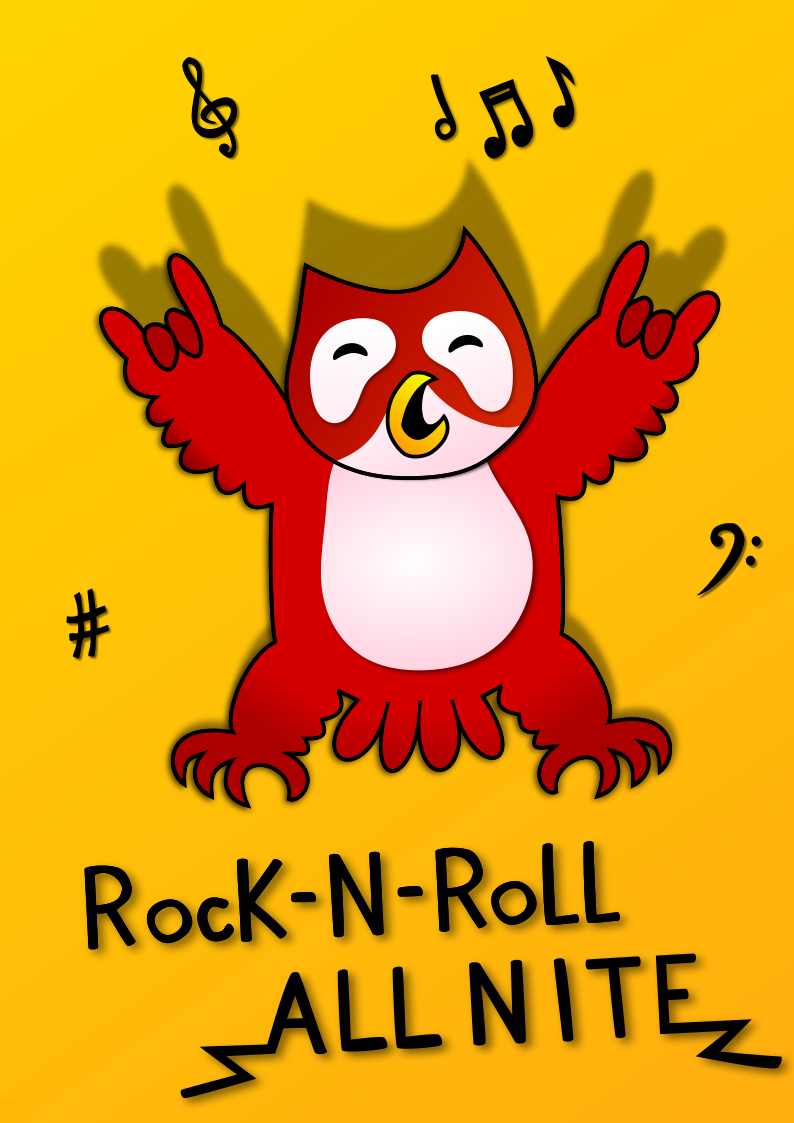
\includepdf[pages={1},offset=2.5cm -2.55cm]{rect1000.png}
%\mainmatter
\mbox{}
\thispagestyle{empty}
\newpage
Страница с благодарностями!\\

Исходный код: github.com/paantya/ska3ka \\
\newpage
\begin{song}{Вожатский гимн}{}{~}{Сказочные}{}{}

По \Ch{Am}{ла}герю подъём, нас горн зовёт!\par
Забудь о том, что ночь была бес\Ch{C}{сон}ною\par
Смо\Ch{Dm}{чи} водою \Ch{G}{ве}ки воспа\Ch{C}{лён}\Ch{F}{ные}\par    
По\Ch{Dm}{вя}зывай свой \Ch{E}{галс}тук — и впе\Ch{Am (A7)}{рёд!}\par
Смо\Ch{Dm}{чи} водою \Ch{G}{ве}ки воспа\Ch{C}{лён}\Ch{F}{ные}\par    
По\Ch{Dm}{вя}зывай свой \Ch{E}{галс}тук — и впе\Ch{Am (A7)}{рёд!}\par

%	\begin{SBChorus*}
\ttНе\Ch{E}{про}сто воспитывать \Ch{Am}{но}вых людей,\par
\ttНу \Ch{E}{что} ж, это наша с то\Ch{Am}{бою} свя\Ch{A7}{ты}ня.\par
\ttМой \Ch{Dm}{друг}, нам до\Ch{G}{ве}рили \Ch{C}{ду}ши де\Ch{F}{тей},\par
\ttИх \Ch{Dm}{ра}достный \Ch{Am}{смех} нам на\Ch{E}{гра}да от\Ch{Am}{ны}не.\par
\ttМой \Ch{Dm}{друг}, нам до\Ch{G}{ве}рили \Ch{C}{ду}ши де\Ch{F}{тей},\par
\ttИх \Ch{Dm}{ра}достный \Ch{Am}{смех} нам на\Ch{E}{гра}да от\Ch{Am}{ны}не.\\
%\end{SBChorus*}

Отбой, засыпает детвора.\par
Взгляни на их улыбки полусонные,\par
Пускай им снятся острова зелёные,\par
А нам опять работать до утра!\par
Пускай им снятся острова зелёные,\par
А нам опять работать до утра!\par

\tt И пусть от бессилья затихнешь не раз,\par
\ttИ голос усталый до хрипа натружен,\par
\ttПусть будут умней и счастливее нас\par
\ttТе дети, в которых вложили мы души!\par
\ttПусть будут умней и счастливее нас\par
\ttТе дети, в которых вложили мы души!

\end{song}

%\twocolumn
\begin{song}{Вожатский марш}{}{~}{Сказочные}{}{}

Есть на\Ch{Am}{род} у нас весёлый,\par
Самой \Ch{C}{луч}шей в мире пробы,\par
Песни \Ch{G}{петь} всегда мас\Ch{C}{так.}\Ch{A7}{}\par
Он всег\Ch{Dm}{да} всего добьётся,\par
Он Вожа\Ch{Am}{ты}ми зовётся,\par
\Ch{E}{Так} и только \Ch{Am (A7)}{так!}\par
Он всег\Ch{Dm}{да} всего добьётся,\par
Он Во\Ch{Am}{жа}тыми зовётся,\par
\Ch{E}{Так} и только \Ch{Am (A7)}{так!}\\

Домосед привязан к дому\par
И по случаю такому,\par
Он из дома — ни на шаг!\par
А вожатый — он в дороге,\par
Он готов в огонь и в воду,\par
Так и только так!\par
А вожатый — он в дороге,\par
Он готов в огонь и в воду,\par
Так и только так!\\
\newpage
Жадный денежки считает,\par
Все считает и считает,\par
К пятаку кладет пятак.\par
А вожатый деньги тратит,\par
Не боясь, что их не хватит,\par
Так и только так!\par
А вожатый деньги тратит,\par
Не боясь, что их не хватит,\par
Так и только так!\\

Холостяк в любовь не верит,\par
Все не верит и не верит,\par
Потому что холостяк.\par
А вожатых не влюблённых\par
Не найдёшь определённо,\par
Так и только так!\par
А вожатых не влюблённых\par
Не найдёшь определённо,\par
Так и только так!\par

\begin{SBSection*}
\begin{figure}[b!]
\center{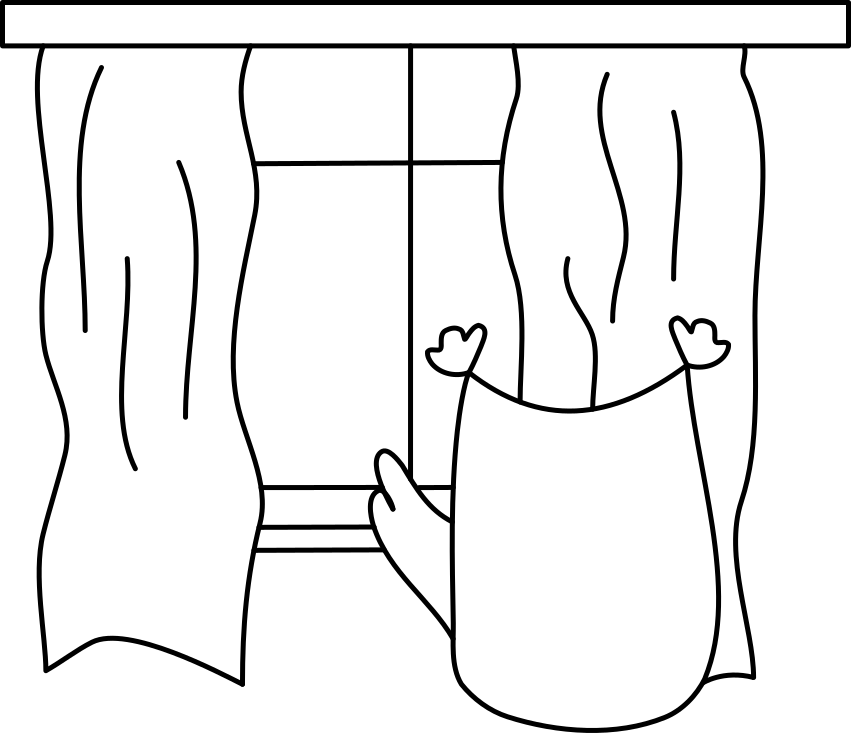
\includegraphics[scale=0.3]{i01}}
\end{figure}
\end{SBSection*}

\end{song}



%\twocolumn
\begin{song}{Двадцать дней}{}{~}{Сказочные}{}{}


Двадцать дн\Ch{Dm}{ей} – это смена без дня.\par
“Маловато”,– вам скажут друзь\Ch{Gm}{я,}\par
А вожатый отв\Ch{C}{ет}ит люб\Ch{F}{ой}:\par
Это ср\Ch{Gm}{ок} очень д\Ch{A}{аж}е больш\Ch{Dm}{ой!}\\
 

Припев:\par
\ttМожно з\Ch{Gm C}{а-а-а-а} него усп\Ch{Dm}{ет}ь,\par
\ttНаприм\Ch{Gm}{ер,} полмилли\Ch{A}{он}а песен сп\Ch{Dm}{еть,}\par
\ttНо не к\Ch{Gm}{ажд}ый ведь поймет,\par
\ttКак так быстро раскрыв\Ch{A}{ат}ься может р\Ch{Dm}{от!}\\


Для полярника это не срок:\par
Не успеет просохнуть носок.\par
А вожатый успеет подряд \par
Вымыть, высушить сотню ребят!\\

Припев:\par
\ttВедь за смену, как за год \par
\ttСтолько разных мелочей произойдет,\par
\ttНо пока что нам везет,\par
\ttНас начальство для чего-то бережёт.\\


\newpage
Хоть и длинными кажутся дни,\par
Но как миг пролетели они.\par
Будешь долго потом вспоминать,\par
Как в отбой ты любил слово «СПАААТЬ!!!»\\

Припев:\par
\tt          	— Говорят за двадцать дней \par
\tt          	Все узнаешь о напарнице своей…\par
\tt          	— Только это ерунда,\par
\tt          	Обо всем ты не узнаешь никогда!\\

Смена вряд ли даст ответ:\par
Ты нашел свое призванье или нет.\par
Так что надо продолжать,\par
Двадцать раз по двадцать суток отсчитать!\\

\begin{SBSection*}
\begin{figure}[b!]
\center{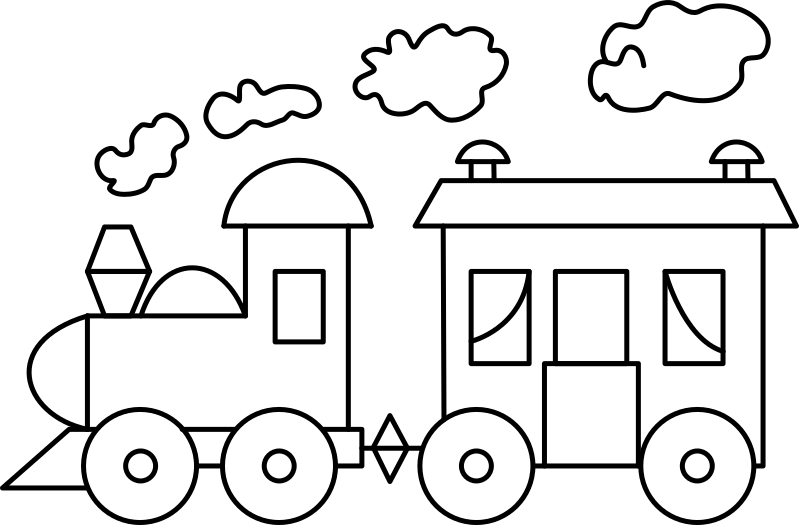
\includegraphics[scale=0.3]{i02}}
\end{figure}
\end{SBSection*}

\end{song}


%\twocolumn
\begin{song}{Непогода}{}{Павел Смеян}{Павел Смеян}{}{}

\Ch{D}{Из}менения в природе \Ch{G}{пр}оисходят г\Ch{A}{од} от года,\par
\Ch{D}{Не}погода нынче в моде,\Ch{G}{} н\Ch{F#7}{епог}ода, непогода,\par
\Ch{}Hm{Слов}но из вод\Ch{F#7}{опро}вода \Ch{D7}{ль}ёт на нас с неб\Ch{G}{ес} во\Ch{Hm}{да…}\par
Полг\Ch{G}{од}а плох\Ch{A}{ая} пог\Ch{D}{од}а, \Ch{Hm}{пол}го\Ch{G}{да} — совс\Ch{A}{ем} нику\Ch{D}{да}.\par
Полг\Ch{G}{од}а плох\Ch{A}{ая} пог\Ch{D}{од}а, \Ch{Hm}{пол}го\Ch{G}{да} — сов\Ch{F#7}{сем} нику\Ch{Hm}{да.}\\


\SBChorusTagg:\par
\ttНикуда, нику\Ch{Em}{да н}ельз\Ch{A}{я} укр\Ch{D}{ы}ться н\Ch{Hm}{ам,}\par
\ttНо откладывать ж\Ch{Em}{изнь} ни\Ch{A}{как} нель\Ch{D}{зя}, \Ch{Hm}{}\par
\ttНикуда, нику\Ch{Em}{да, н}о зн\Ch{A}{ай}, что гд\Ch{D}{е}-то т\Ch{Hm}{ам}\par
\ttКто-то ищет теб\Ch{G}{я} сре\Ch{F#7}{ди д}ожд\Ch{Hm}{я.} \Ch{A}{}\\


Грома грозные раскаты от заката до восхода,\par
За грехи людские плата — непогода, непогода,\par
Не ангина, не простуда, посерьёзнее беда.\par
Полгода плохая погода, полгода — совсем никуда\par,
Полгода плохая погода, полгода — совсем никуда.\\\


\SBChorusTagg:\par
\ttНикуда, нику\Ch{Em}{да н}ельз\Ch{A}{я} укр\Ch{D}{ы}ться н\Ch{Hm}{ам,}\par
\ttНо откладывать ж\Ch{Em}{изнь} ни\Ch{A}{как} нель\Ch{D}{зя}, \Ch{Hm}{}\par
\ttНикуда, нику\Ch{Em}{да, н}о зн\Ch{A}{ай}, что гд\Ch{D}{е}-то т\Ch{Hm}{ам}\par
\ttКто-то ищет теб\Ch{G}{я} сре\Ch{F#7}{ди д}ожд\Ch{Hm}{я.} \Ch{A}{}\\


\end{song}

%\twocolumn
\begin{song}{Птенцы}{}{~}{Сказочные}{}{}

\Ch{Am}{}  \Ch{Am}{}

Как птенцы из гнез\Ch{Dm}{да} мы \Ch{E}{вы}па\Ch{Am}{ли.}\par
Ты не бойся при\Ch{Dm}{хо}да \Ch{G}{ве}че\Ch{C}{ра.}\par
Под та\Ch{A7}{ки}ми боль\Ch{F}{ши}ми \Ch{A7}{ли}па\Ch{Dm}{ми}\par
Нам с то\Ch{F}{бой} опа\Ch{Dm}{сать}ся \Ch{F}{не}\Ch{E}{че}\Ch{Am}{го.}\\
 
Под такими густыми звёздами -\par
Разве их не для нас рассыпали,\par
Мы не против гнездовья - просто мы\par
Из него ненароком выпали.\\

Это только вначале кажется,\par
Что без дома прожить нельзя никак,\par
Что важней пропитанья кашица,\par
Чем огромные звёзды на небе.\\

Ты не бойся ни тьмы, ни холода.\par
Будет день и найдётся пища нам,\par
Мы ещё пролетим над городом\par
На крыле до небес возвышенном.\\

Пролетим ещё - эка невидаль\par
Над Нью-Йорком, Парижем, Триполи\par
И над липой, откуда некогда,\par
Как птенцы из гнезда мы выпали.\\

Как птенцы из гнезда мы выпали.\par
Ты не бойся прихода вечера.\par
Под такими большими липами\par
Нам с тобой опасаться нечего.\\

\end{song}

%\twocolumn
\begin{song}{Продавец зонтиков}{}{Веня Дркин}{Веня Дркин}{}{}

\Ch{Am}{Город} этот выдумал о\Ch{Dm}{дин} художник,\par
\Ch{G}{Лю}ди в нем не знали, что та\Ch{C}{ко}е дождик.\par
\Ch{A7}{Про}сто не слыхали, что та\Ch{Dm}{ко}е зонтик –\par
\Ch{E7}{Вот} такие люди жили в \Ch{Am}{го}роде том.\par
И один чудак, в старый плащ одетый,\par
Продавал там зонтики зимой и летом,\par
Продавал там зонтики зимой и летом\par
И такую песенку он напевал:\\

\SBChorusTagg:\par
\tt“Господа, купите зонтик.\par
\ttБелый зонтик, красный зонтик,\par
\ttЖелтый зонтик, синий зонтик –\par
\ttМожет пригодится вам.”\\

Были домики у них из пластилина,\par
Из пустых коробочек автомашины,\par
И, не опасаясь никакой ангины,\par
Маленькие люди жили в городе том.\par
Маленькие были у людей заботы:\par
Шли они в кино или в театр с работы.\par
Вечером в подъезде целовался кто-то.\par
Все шутили и смеялись над стариком.\\


\SBChorusTagg.\\

\newpage

Маленькое небо как-то вдруг намокло,\par
В крошечных домишках задрожали стекла,\par
И огромный дождь пошел гулять по крышам,\par
Сразу все схватили насморк в городе том.\par
Вспомнили тут люди о торговце старом,\par
Кинулись искать его по всем базарам,\par
Но исчез торговец со своим товаром.\par
Только песенка осталась в память о нем:\\

\SBChorusTagg.\par

\begin{SBSection*}
\begin{figure}[b!]
\center{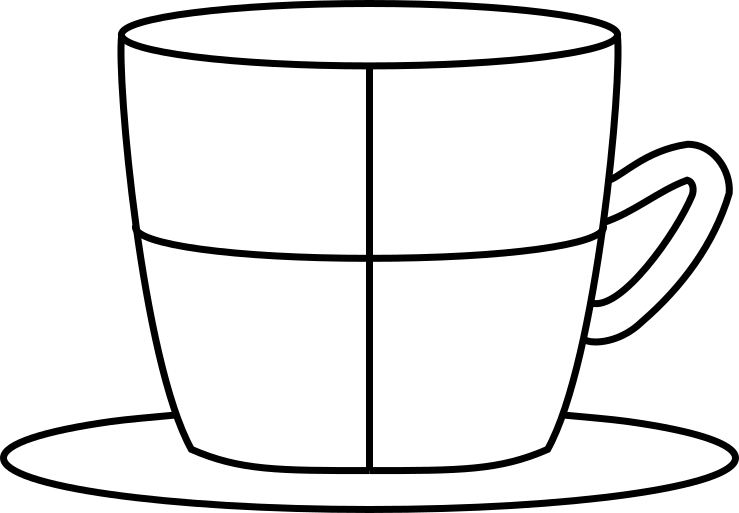
\includegraphics[scale=0.4]{i03}}
\end{figure}
\end{SBSection*}

\end{song}

%\twocolumn
\begin{song}{Белая гвардия}{}{Белая гвардия}{Белая гвардия}{}{}

Проигрыш: (2 раза)\par 
\Ch{Am}{} \Ch{D}{} \Ch{G}{} \Ch{C}{} \Ch{Am}{} \Ch{H7}{} \Ch{Em}\\

\Ch{Em}{Белая} гвардия, белый снег,\par
\Ch{Am7}{Белая} музыка революций.\par
\Ch{D7}{Белая} женщина, нервный смех,\par
\Ch{G}{Белого} платья слегка коснуться.\par
 
Белой рукой распахнуть окно,\par
Белого света в нем не видя.\par
Белое выпить до дна вино,\par
В красную улицу в белом выйти.\\

Припев:\par
\ttКог\Ch{Em}{да} ты вернешься,\par
\ttВсе будет и\Ch{Am}{на}че, и нам бы узнать друг друга,\par
\ttКог\Ch{D7}{да} ты вернешься,\par
\ttА я не же\Ch{G}{на} и даже \Ch{H7}{не} подруга.\par
\ttКог\Ch{C}{да} ты вернешься,\par
\ttКо мне, так без\Ch{Am}{ум}но тебя любившей в прошлом,\par
\tt\Ch{D7}{Ко}гда ты вернешься -\par
\ttУвидишь, что ж\Ch{G}{ре}бий давно и не \Ch{E7}{нами} брошен.\\

Проигрыш.\\
 
\newpage
Сизые сумерки прошлых лет\par
Робко крадутся по переулкам.\par
В этом окне еле брезжит свет,\par
Ноты истрепаны, звуки гулки.\par
Тонкие пальцы срывают аккорд...\par
Нам не простят безрассудного дара.\par
Бьются в решетку стальных ворот\par
Пять океанов земного шара.\\

Припев. \par
Проигрыш.\\
 
Красный трамвай простучал в ночи,\par
Красный закат догорел в бокале,\par
Красные-красные кумачи\par
С красных деревьев на землю упали.\par
Я не ждала тебя в октябре,\par
Виделись сны, я листала сонник:\par
Красные лошади на заре\par
Били копытами о подоконник.\\

Припев:\par
\ttКогда ты вернешься,\par
\ttВсе будет иначе, и нам бы узнать друг друга,\par
\ttКогда ты вернешься,\par
\ttА я не жена и даже не подруга.\par
\ttКогда ты вернешься,\par
\ttВернешься в наш город обетованный,\par
\ttКогда ты вернешься -\par
\ttТакой невозможный и такой желанный?\\

Проигрыш.\par


\end{song}


%\twocolumn
\begin{song}{Ленинградская (Все расстояния)}{}{~}{Лагерные}{}{}

\Ch{Am}{Все} расстоянья когда-нибудь в круг замы\Ch{E}{ка}ются,\par
\Ch{E}{Все} из разлук обязательно \Ch{E7}{встре}чей кон\Ch{Am}{ча}ются;\par
Должны про\Ch{Dm}{плыть} вокруг Зем\Ch{G}{ли,}\par
Вернуться в \Ch{C}{га}вань кораб\Ch{F}{ли,}\par   
Все поез\Ch{Dm}{да} в свои вер\Ch{E}{нуть}ся горо\Ch{Am}{да.}\\
 
Шумный вокзал то встречает друзей , то прощается,\par
Мы расстаемся, но снова назад возвращаемся -\par
Чтоб снова встать в огромный круг,\par
И снова знать, что рядом друг ,\par
И песни петь, чтоб больше не было разлук.\\
 
Все расстоянья когда-нибудь в круг замыкаются,\par
Все из разлук обязательно встречей кончаются;\par
И через год, и через пять,\par
Мы с вами встретимся опять,\par
Ничто не сможет нашей дружбе помешать.\par

\end{song}

\begin{song}{Фрагмент}{}{О. Митяев}{О. Митяев}{}{}

Тронется, еще чуть-чуть, - и поезд тронется.\par
И с печальным вздохом тихо дверь закроется.\par
Вянет ночь, сирень ее становится прозрачною,\par
И среди чужих твое теряется лицо.\\
 
Мелочью стучится дождь в стекло, бегут кусты,\par
На холсте окна пейзаж размыт, и взгляд застыл.\par
И скользят артерии рябин по холоду\par
Сквозь немую ярмарку сорвавшейся листвы.\\
 
Припев (перебором):\\

Тихо листопад закружит сад и уже не повернуть назад,\par
Канет осень в снег, как в соболя венчанная женщина.\par
Поплывет из серой тишины пеной на пожарище травы,\par
Запорошит отраженья рек снег…\\
 
Все забыть, смотреть в глаза и больше не спешить.\par
И за этот миг, совсем недолгий, жизнь прожить.\par
Шаг шагнуть в дверной проем и перестать дышать,\par
И не думать ни о чем, смотреть сквозь снег и ждать…\\

 
Припев\\

Тpонется, еще чуть-чуть и поезд тpонется...

\end{song}

\begin{song}{Перевал}{}{~}{Лагерные}{}{}

\Ch{Am}{Про}сто нечего нам \Ch{Dm}{боль}ше терять\par
\Ch{E}{Всё} нам вспомнится на \Ch{Am}{Страшном} суде.\par
Эта ночь легла, как \Ch{Dm}{тот} перевал,\par
\Ch{G}{За} которым испол\Ch{C}{нень}е надежд.\par
\Ch{A7}{Про}сто прожитое—про\Ch{Dm}{жи}то зря, \Ch{G}{}\par
Но не в этом, пони\Ch{C}{мае}шь ли, соль… \Ch{Am}{}\par
Слышишь, падают дож\Ch{Dm}{ди} октября.\par
\Ch{E}{Ви}дишь, старый дом сто\Ch{Am}{ит} средь лесов.\\

Мы затопим в доме печь, в доме печь,\par
Мы гитару позовем со стены.\par
Просто нечего нам больше беречь,\par
Ведь за нами все мосты сожжены.\par
Все мосты, все перекрёстки дорог,\par
Все прошёптанные тайны в ночи.\par
Каждый сделал все, что смог, все, что смог,\par
Мы об этом помолчим, помолчим.\\


И луна взойдет заплывшей свечой,\par
Ставни скрипнут  на ветру, на ветру.\par
Ах, как я тебя люблю горячо,\par
Это годы не сотрут, не сотрут.\par
Мы оставшихся друзей соберем,\par
Мы набьем картошкой старый рюкзак,\par
Люди спросят: "Что за шум, что за гам?"\par
Мы ответим: "Просто так,  просто так”...\\


\newpage
    Просто так идут дожди в октябре,\par
    И потеряны от счастья ключи.\par
    Это всё, конечно, мне, конечно, мне,\par
    Но об этом помолчим, помолчим.\par
    Просто прожитое—прожито зря,\par
    Но не в этом, понимаешь ли, соль…\par
    Слышишь, падают дожди октября.\par
    Видишь, старый дом стоит средь лесов.\\
    
   \begin{SBSection*}
\begin{figure}[b!]
\center{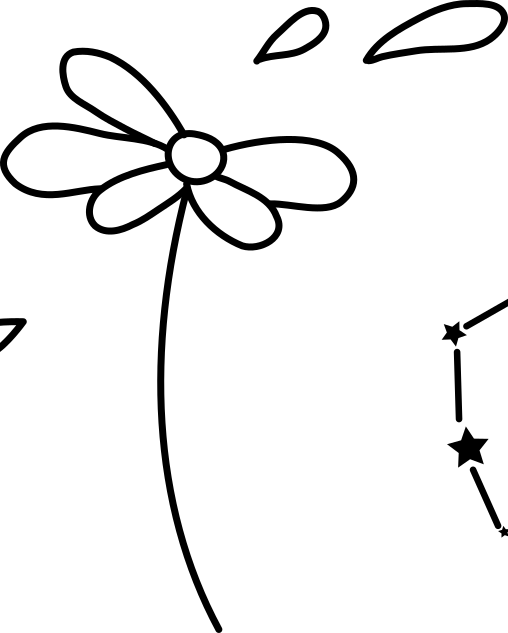
\includegraphics[scale=0.4]{i04}}
\end{figure}
\end{SBSection*}
\end{song}

\begin{song}{Прекрасное далёко}{}{из к/ф “Гостья из будущего”}{из к/ф “Гостья из будущего”}{}{}

Слышу г\Ch{Am}{оло}с из прекрасного дал\Ch{Dm}{ёка}\par        	
Голос \Ch{E}{у}тренний в сер\Ch{E}{е}бряной ро\Ch{Am}{се}\par
Слышу г\Ch{F}{о}лос, и ман\Ch{G7}{ящ}ая дор\Ch{C}{о}га \Ch{Am}{}\par
Кружит г\Ch{F}{о}лову, как в д\Ch{F7}{ет}стве карус\Ch{E}{е}ль.\\
 
Припев:\par
\ttПрекр\Ch{Am}{асн}ое дал\Ch{Dm}{ёко,} не б\Ch{E}{у}дь ко мне жесто\Ch{Am}{ко,}\par
\ttНе б\Ch{F}{у}дь ко мне жест\Ch{C}{о}ко, жест\Ch{G7}{о}ко не б\Ch{C}{у}дь. \Ch{E}{}\par
\ttОт ч\Ch{Am}{ист}ого ист\Ch{Dm}{ока} в прекр\Ch{E}{а}сное дал\Ch{F}{ё}ко,\par
\ttВ прекр\Ch{Dm}{асн}ое дал\Ch{Am}{ёко} я н\Ch{E7}{ач}инаю п\Ch{Am}{уть.}\\
 
Слышу голос из прекрасного далёка,\par
Он зовет меня не в райские края.\par
Слышу голос, голос спрашивает строго:\par
А сегодня что для завтра сделал я?\\
 
Припев.\\
 
Я клянусь, что стану чище и добрее,\par
И в беде не брошу друга никогда.\par
Слышу голос, и спешу на зов скорее,\par
По дороге, на которой нет следа.\\
 
Припев.\\

\end{song} 

\begin{song}{Песня бременских музыкантов}{}{из м/ф “Приключения бременских музыкантов”}{из м/ф “Приключения бременских музыкантов”}{}{}

Нич\Ch{C}{е}го на свете луч\Ch{Em}{ше н}ету,\par
Че\Ch{F}{м} бродить друзьям по белу с\Ch{G}{в}ету.\par
Те\Ch{C}{м,} кто дружен, не ст\Ch{Am}{раш}ны тревоги,\par
Н\Ch{Dm}{ам} любые д\Ch{G}{о}роги дор\Ch{C}{о}г\Ch{F}{и.}\par
Н\Ch{Dm}{ам} любые дор\Ch{G}{о}ги дор\Ch{C}{о}гиииии.\\

На на на н\Ch{Am}{ана}й на на на н\Ch{Dm}{айн}а на на на \Ch{G}{е} е е е е\\
 
Наш ковер - цветочная поляна\par
Наши стены - сосны-великаны\par
Наша крыша - небо голубое\par
Наше счастье - жить такой судьбою.(2раза)\\
 
Мы свое призванье не забудем,\par
Смех и радость мы приносим людям!\par
Нам дворцов заманчивые своды\par
Не заменят никогда свободы. (2 раза)\\

На на на н\Ch{Am}{ана}й на на на н\Ch{Dm}{айн}а на на на н\Ch{G}{а}нанана най\par
На на на н\Ch{C}{а}йна на на на н\Ch{Am}{ана}нана най\par
На на на н\Ch{Dm}{ана}й на на на \Ch{G}{е} е е е е\\
 
\end{song}



\begin{song}{Чудо}{}{В. Егоров}{В. Егоров}{}{}

Б\Ch{Em}{елы}е дороги, белые дома, зима.\par
На дворе снега, стоят из снега тере\Ch{Am}{ма.}\par                
Для детей они слет\Ch{D}{ел}и с неба,\par                             	
М\Ch{G}{ы-}то с вами знаем, что он\Ch{C}{и} из снега,\par
М\Ch{Am}{ы-т}о с вами не сошли с у\Ch{	H7}{ма.}\par
А у сказки краски, словно витражи, свежи.\par
Только не для нас, ведь мы на вираже уже.\par
Наши сказки серые от пыли,\par
Потому что мы когда-то юны были,\par
А теперь не юные уже.\\

\ttС\Ch{Em}{ын} прижал по\Ch{Em}{душк}у щекой,\par
\ttЕго с\Ch{D7}{он} — невозмут\Ch{G}{и}мый покой,\par
\ttВысок\Ch{C}{о} взлетает м\Ch{Am}{але}нький Мук,\par
\ttБаб\Ch{H7}{а-}Яга и Змей Горыныч,\par
\ttА за ним Синдбад, а потом\par
\ttМаркиз Карабас в обнимку с Котом\par
\ttХоджа Насреддин с ослом, а потом…\par
\ttКороче, всех не перечислишь…\\

Когда мы были лопоухие щены,\par
В сказке, как в купели все мы были крещены.\par
В сказке как в купели мы плескались,\par
Маленькими песни пели и смеялись\par
И не знали этому цены.\\

\newpage
В сны детей поверить нам хоть на полчаса\par
Слава Богу есть свои у взрослых чудеса:\par
Чудо обитает в чаще леса,\par
 Чудо проживает в глубине Лох-Несса,\par
Чудо проплывает в небесах...\\

\ttВ синих Гималайских снегах \par
\ttБродит чудо, бродит чудо на мохнатых ногах \par
\ttБродит чудо, оставляя следы \par
\ttСемидесятого размера,\par
\ttА за ним снега и века,\par
\ttЛьется в небо, льется в небо, голубая река \par
\ttИ стремительно плывут облака \\

Очень похожие на блюдца.\par
Чудо, чудо, чудо — вечный для людей магнит.\par
Чудо Атлантиды дразнит и к себе манит.\par
Словно бы ракета перед пуском,\par
Огненное чудо над тайгой Тунгуской \par
Свой секрет почти 100 лет хранит.\par
Сказки пожелтели, сказки облетели, но \par
В сказку никогда не поздно распахнуть окно.\par
Только вы аршином мир не мерьте,\par
Только вы поверьте, только вы поверьте \par
В то, что мы поверили давно…\\

\ttВ то, что чудо рядом лежит,\par
\ttЕще в то, что нам без чуда не жить,\par
\ttИ тогда однажды вечером к вам \par
\ttОно слетит на подоконник,\par
\ttА за ним Синдбад, а потом \par
\ttМаркиз Карабас в обнимку с Котом,\par
\ttХоджа Насреддин с ослом, а потом…\par
\ttКороче всех не перечислишь…\par
\ttОчень похожие на блюдца…\\
\end{song}


\begin{song}{Алые паруса}{~}{~}{Лагерные}{}{}

У с\Ch{C}{и}него моря \par
Где буш\Ch{Am}{уют} бураны,\par
Жил\Ch{F}{а} там девчонка \par
С \Ch{G}{и}менем странным.\par
И часто бывало \par
Она на просторе \par
В мечтах уплывала \par
За синее море.\\

Припев:(2 раза)\par
\tt\Ch{C}{А}лые п\Ch{Am}{ару}са!\par
\tt\Ch{C}{А}лые п\Ch{Am}{ару}са!\par
\tt\Ch{F}{А}лые п\Ch{G}{а}руса, парус\Ch{C}{а.}\par
\ttРаз! Дв\Ch{G}{а}! Три!\\
 
А там за морями \par
За синей чертою \par
Жил парень чудесный \par
С открытой душою.\par
Мечтал о море,\par
О подвигах славных,\par
В мечтах уплывал он \par
В далекие страны.\\

\newpage

Припев.\\
 
А вечером поздним,\par
Когда все уснули,\par
На небе зажглись \par
Гирлянды огней.\par
И этой же ночью \par
Случилося чудо:\par
Тот парень приехал \par
К девчонке своей.\\

Припев.\\

\begin{SBSection*}
\begin{figure}[b!]
\center{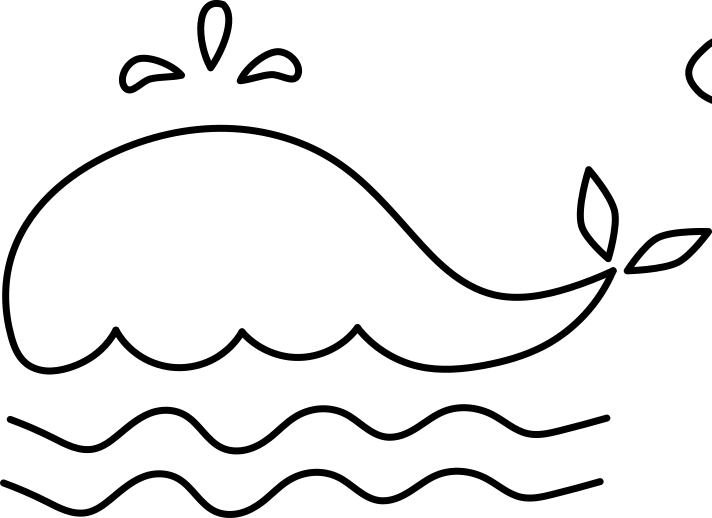
\includegraphics[scale=0.4]{i05}}
\end{figure}
\end{SBSection*}

\end{song}


\begin{song}{Вечер бродит}{}{А. Якушева}{А.Якушева}{}{}

В\Ch{Am}{ече}р бр\Ch{Dm}{оди}т п\Ch{E}{о} лесным дор\Ch{Am}{ожк}ам,\par
Т\Ch{Am}{ы в}едь т\Ch{Dm}{оже} любишь в\Ch{G}{е}чер\Ch{C}{а,}\par
П\Ch{A7}{од}ожд\Ch{Dm}{и, п}ост\Ch{G}{о}й ещ\Ch{C}{ё} немножко,    	(1-й голос)\par
Подожди, посто-о-ой ещё немножко,     							(2-й голос)\par
П\Ch{Dm}{оси}дим с то\Ch{Am}{вари}щами \Ch{E}{у} костр\Ch{Am}{а.}  	(1-й голос)\par
По-о-о- сиди-и-м мы у костра.         							(2-й голос)\\
 
Вижу целый мир в глазах тревожных \par
В этот час на берегу крутом,\par
Не смотри ты так неосторожно,   	    (1-й голос)\par
Не смотри ты та-a-к неосторожно,     (2-й голос)\par
Я могу подумать что-нибудь не то.    (1-й голос)\par
Я-а-а поду-у-у маю не то.            (2-й голос)\\
 
Ясный месяц на прогулку вышел,\par
Звёзды смотрят из глубин небес,\par
Друг хороший, ты меня услышишь, 		(1-й голос)\par
Друг хороший, ты-ы меня услышишь, 	(2-й голос)\par
Эту песню я пою сейчас тебе. 		(1-й голос)\par
Э-э-эта пе-e-eсня о тебе. 			(2-й голос)\\
 
Что волшебней задушевной песни,\par
И заката в отблесках огня,\par
Нет на свете глаз твоих чудесней, 	(1-й голос)\par
Нет на свете гла-а-аз твоих чудесней, 	(2-й голос)\par
Что глядят задумчиво так на меня. 	(1-й голос)\par
Что-о-о глядя-а-ат так на меня. 		(2-й голос)\\
 
Вслед за песней позовут ребята\par
В неизвестные ещё края,\par
И тогда над крыльями заката           	(1-й голос)\par
И тогда над кры-ы-ы-льями заката    	(2-й голос)\par
Вспыхнет яркой звёздочкой мечта моя   (1-й голос)\par
Вспы-ы-ыхнет звё-ё-ёздочка моя.   	(2-й голос)\\
 
Знаю, будут и другие встречи,\par
Незаметно пролетят года,\par
Но вот этот тихий тёплый вечер 		(1-й голос)\par
Но вот этот ти-и-ихий тёплый вечер    	(2-й голос)\par
Мы с тобою не забудем никогда. 		(1-й голос)\par
Не-е-е забу-у-удем никогда. 		(2-й голос)\\

\begin{SBSection*}
\begin{figure}[b!]
\center{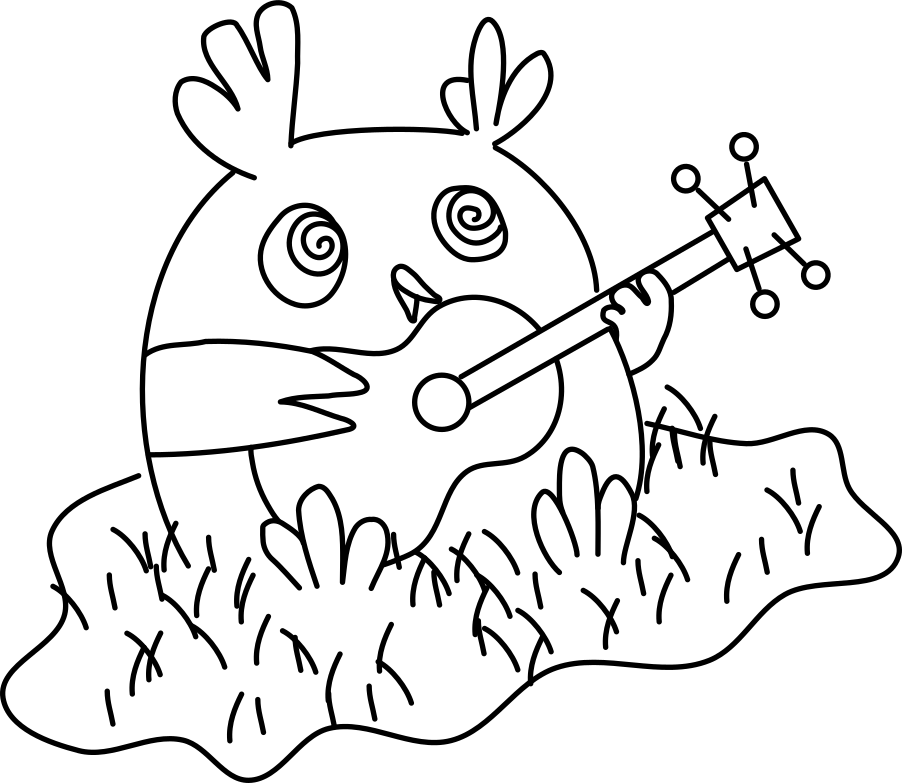
\includegraphics[scale=0.4]{i06}}
\end{figure}
\end{SBSection*}
\end{song}


\begin{song}{На ранчо}{}{~}{Лагерные}{}{}

В \Ch{C}{} далёких Кордильерах, на с\Ch{F}{е}вере Техаса,\par
Сто\Ch{C}{я}ло одинокое ран\Ch{G}{ч}о, о-о!\par
Стар\Ch{C}{у}шка там жила крив\Ch{F}{а} и одноглаза,\par
Гус\Ch{C}{е}й она корм\Ch{G}{и}ла саранчо\Ch{C}{й}.\\

Припев:\par
\tt             На р\Ch{C}{а}нчо, на ранчо, ск\Ch{F}{о}ро я вернуся\par
\tt             Ж\Ch{C}{и}ли-были два гуся \Ch{G}{у} одной баб\Ch{C}{у}си.\\

На лошади гнедой, с семизарядным кольтом,\par
Она гоняла в прерии гусей, е-ей!\par
И крохотный загон с проводкой в 200 вольтов \par
Их охранял, чтоб не украл сосед \par
А по соседству жил огромнейший верзила \par
Он виски жрал как лошадь, и притом, о-ом!\par
Он звался "Черный Билл", и будучи один он,\par
Считался первым парнем на ранчо.\\

Припев.\\

Раз как-то поутру, как только солнце встало,\par
И в прериях рассеялся туман, а-ан!\par
Старушка двух гусей, увы, не досчиталась,\par
А это, вы поймите, не фонтан\par
Вскипела в жилах кровь у маленькой старушки,\par
Она хватает кольт свой поскорей, е-ей!\par
Вгоняет в ствол патрон и - к Билловой избушке\par
Готовая к изъятию гусей.\\

Припев.\\

Вот выстрел прогремел, и дрогнула хибара..\par
И Черный Билл едва успел сказать: “Брррр!\par
На черта гуси мне? А это – кукабара,” -\par
На кости кукабары он упал.\par
     Старушка мчится прочь к племяннику в Монтану,\par
     Поскольку поломата жизня вся, а-а!\par
     Кругом ночная мгла, как вдруг из-под банана \par
     Навстречу ей выходят два гуся.\par
М\Ch{F}{ы}ли гуси л\Ch{C}{а}пки в л\Ch{F}{у}же у кан\Ch{C}{а}вки,\par
\Ch{F}{О}дин серый, др\Ch{C}{у}гой белый,\par
Cпр\Ch{G}{я}тались от б\Ch{C}{а}бки! \\
 
Припев.\\

\begin{SBSection*}
\begin{figure}[b!]
\center{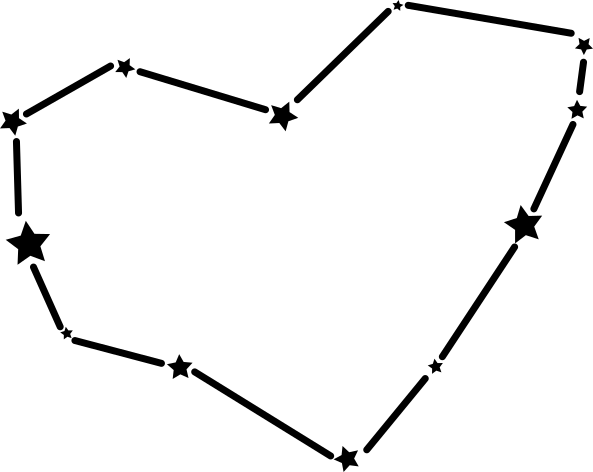
\includegraphics[scale=0.3]{i07}}
\end{figure}
\end{SBSection*}
\end{song}


\begin{song}{Луч солнца золотого}{}{из м/ф “Приключения бременских музыкантов”}{из м/ф “Приключения бременских музыкантов”}{}{}

Лу\Ch{C}{ч} солнца золот\Ch{Em}{ого}\par
Тьм\Ch{F}{ы} скрыла пелен\Ch{G}{а.}\par
\Ch{C}{И} между нами сн\Ch{Em}{ова}\par
Вдр\Ch{F}{у}г выросла стен\Ch{G}{а.}\\
 
Проигрыш: C Am F G\\
 
Припев:\par
\tt\Ch{C}{Н}очь пройд\Ch{Am}{ёт,} наступит \Ch{F}{у}тро \Ch{G}{я}сное,\par
\tt\Ch{C}{З}наю, сч\Ch{Am}{асть}е нас с тоб\Ch{F}{о}й жд\Ch{G}{ё}т.\par
\tt\Ch{C}{Н}очь пройд\Ch{Am}{ёт,} пройдет пор\Ch{F}{а} нен\Ch{G}{а}стная,\par
\tt\Ch{C}{С}олнце взойд\Ch{Am}{ёт!}(2 \Ch{F}{р}аза)\Ch{G}{}\\
 
Петь птицы перестали,\par
Свет звезд коснулся крыш.\par
В час грусти и печали\par
Ты голос мой услышь. \\

Припев.\\

\end{song} 

\begin{song}{Лягушка}{}{~}{Лагерные}{}{}

Ш\Ch{Am}{ёл }парнишка по опушке, сам не знал к\Ch{Dm}{уда.}\par
П\Ch{Am}{о пу}ти нашел лягушку около пру\Ch{Dm}{да}\par
И взглянув в глаз\Ch{G}{а}, она сказала вд\Ch{Am}{руг}\par
\Ch{Dm}{"Отп}усти мен\Ch{E7}{я }на свободу др\Ch{Am}{уг.}\\
 
Припев:(2 раза)\par
\ttТр\Ch{A7}{еб}уй, ч\Ch{Dm}{то т}ебе надо, \Ch{G}{я}, я пом\Ch{C}{о}чь тебе рада \par
\tt\Ch{Am}{И}, и в нагр\Ch{Dm}{аду} исполню \Ch{E}{я} три желанья тво\Ch{Am}{и.}\\

Три желанья мучат парня, выбрать он не смог.\par
Пожелал на первый случай золота мешок.\par
И он стал богат, но в душе не рад,\par
Ровно через год вновь к пруду идёт.\\

Припев\\

Пожелал парнишка власти и в краю родном \par
В тот же день он был по праву избран королём.\par
Но не в этом дело, но не в этом суть,\par
Гложит парня всё одна и та же грусть.\\


Припев\\

"Дай ты мне увидеть счатье, сердце озари,\par
Вместо денег, вместо власти дай ты мне любви."\par
И лягушка вмиг изменила вид,\par
Перед ним, смеясь, девушка стоит.\\
\tt"Раз, любви тебе надо, я, я помочь тебе рада (2 раза)\par		
\ttИ, и в награду исполню я все желанья твои.”\\


\end{song}



\begin{song}{Чайка}{}{И.Грибулина}{И.Грибулина}{}{}

К\Ch{Am}{ружи}тся чайка в медленном вальсе над волн\Ch{E}{о}й\par
Вот и настало время прощаться н\Ch{E7}{ам} с то\Ch{Am}{бой}\\
 
Припев:\par
\ttБ\Ch{A7}{уд}ем идти мы, с ветрами споря, за мечт\Ch{Dm}{ой}\par
\ttВерную др\Ch{G}{у}жбу, св\Ch{C}{е}тлые з\Ch{C}{о}ри м\Ch{Dm}{ы у}нес\Ch{E}{ё}м с соб\Ch{Am}{ой.} \Ch{A7}{}\par
\ttВ\Ch{Dm}{ерн}ую др\Ch{G}{у}жбу, св\Ch{C}{е}тлые з\Ch{F}{о}ри м\Ch{Dm}{ы у}нес\Ch{E}{ё}м с соб\Ch{Am}{ой}\\
 
Как часовые сосны застыли вдалеке.\par
Сложатся буквы в чье-нибудь имя на песке.\\
 
Припев.\\
 
Чайка над морем парусом белым проплывет.\par
Прямо в ладони звездочка с неба упадет.\\
 
Припев.\\
 
Доброе лето песнею стало звонких дней.\par
Ждет нас не мало трудных причалов и путей.\\
 
Припев.\\
\end{song}


%\twocolumn
\begin{song}{Десять капель}{}{Танцы Минус}{Танцы Минус}{}{}

Проигрыш: (2 раза)\par 
\Ch{C}{} \Ch{E}{} \Ch{Am}{} \Ch{F}{} \Ch{C}{} \Ch{E}{} \Ch{Am}{} \Ch{F}{}

\Ch{C}{Де}сять капель дож\Ch{E}{дя} у тебя на пле\Ch{Am}{че}\par
Ты забыла свой \Ch{F}{зонт,} ты спешила ко \Ch{C}{мне.}\par
Десять капель дож\Ch{E}{дя} на плече у те\Ch{Am}{бя,}\par
Десять капель люб\Ch{F}{ви,} десять капель ог\Ch{C}{ня}\\

Припев:\\(Три первых слова в припеве дублируются вторым голосом)\par
\tt\Ch{C}{Т}воя\Ch{E}{} ладо\Ch{Am}{нь} горит\Ch{F}{} в моих руках\par
\tt\Ch{C}{Л}юбви\Ch{E}{ }пож\Ch{Am}{ар} горит в тво\Ch{F}{их} глазах\\

Проигрыш.\\

Время делает шаг, время делает круг\par
Мы забудем друзей, мы забудем подруг\par
Просто выпьем вина из любви и огня\par
Десять капель меня, десять капель тебя\\

Припев.\\

Голос твой в тишине околдует меня\par
Ярким жарким огнем стану я до утра\par
Ты прикажешь гори, и я вспыхну любя\par
В этом пламени ты, в этом пламени я.\par

\end{song}

\begin{song}{Семнадцать лет}{}{гр. Чайф}{гр. Чайф}{}{}

\Ch{Am}{Я }ви\Ch{F}{жу}, \Ch{G}{я} снова вижу те\Ch{C}{бя} такой.\par
\Ch{Am}{В де}рзкой мини\Ch{F}{-}юбке, \Ch{G}{чт}о мой по\Ch{G}{кой},\par
\Ch{Am}{Мой} сон,\Ch{F}{ м}ой сон \Ch{G}{ п}ревратили, шу\Ch{C}{тя},\par
\Ch{Am}{В те}бя\Ch{F}{,}\Ch{G}{ я} умоляю теб\Ch{C}{я}:\\
 
Припев:\\

\ttП\Ch{C}{ус}ть все будет \Ch{C7}{та}к, как ты захочешь,\par
\ttП\Ch{F}{ус}ть твои глаза, как п\Ch{Fm}{реж}де, горят.\par
\ttЯ\Ch{C}{ с} тобой опять сег\Ch{Am}{одн}я этой ночью,\par
\ttН\Ch{F}{у} а впрочем, н\Ch{Fm6}{у а в}прочем,\par
\ttС\Ch{C}{ле}дующей ночью, с\Ch{C7}{ле}дующей ночью,\par
\ttЕ\Ch{F}{сл}и захоч\Ch{Fm}{ешь}, я оп\Ch{G}{ят}ь у те\Ch{C}{бя}.\\
 
\newpage
\noindentТебе семнадцать, тебе опять семнадцать лет.\par
\noindentКаждый твой день рожденья хочет прибавить, а я скажу - нет.\par
\noindentТвой портрет, твои дети, я расскажу им о том:\par
\noindent"Д\Ch{Am}{ети}, вашей маме с\Ch{F}{но}ва семнадцать,\par
\noindentВы п\Ch{G}{ро}сто поверьте, а пой\Ch{C}{мё}те потом".\\
 
Припев\\
 
\noindentВазы в нашем доме, в них редко бывают цветы.\par
\noindentВ мае снова будут тюльпаны, я помню, их так любишь ты.\par
\noindentЯ напишу свою лучшую песню, если будет угодно судьбе.\par
\noindentИ первой ее сыграю тебе, конечно, тебе.\\

Припев\\

\begin{SBSection*}
\begin{figure}[b!]
\center{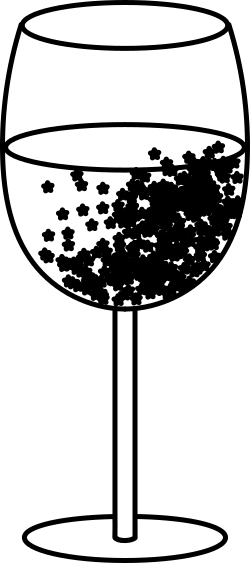
\includegraphics[scale=0.3]{i08}}
\end{figure}
\end{SBSection*}

\end{song}

\begin{song}{Замыкая круг}{}{Крис Кельми}{Крис Кельми}{}{}

\Ch{C}{В}от одна из тех\Ch{F}{ }историй,\par
О кот\Ch{C}{ор}ых л\Ch{Am}{юд}и споря\Ch{F}{т }\par
И не день не д\Ch{Fm}{ва}, а много лет.\Ch{C}{  }\par
Началась он\Ch{F}{а }так просто\par
Не с отв\Ch{C}{ет}ов, а с вопросов\Ch{F}{, }\par
До сих пор на н\Ch{Fm}{их} ответов нет\Ch{C}{: }\\

Почему стремятся к свету\par
Все растения на свете?\par
Отчего к морям спешит река?\par 
Как мы в этот мир приходим?\par
В чем секрет простых мелодий?\par
Нам хотелось знать наверняка.\\

Припев:\\

\ttЗамы\Ch{F}{ка}я кру\Ch{G}{г,}\par 
\ttТы на\Ch{Em}{зад} посмотришь вдру\Ch{Am}{г.}\par
\ttТам увидишь в \Ch{Dm}{окн}ах свет,\par
\ttС\Ch{G}{ия}ющий нам всл\Ch{C}{е}д.\par
\ttПусть иду\Ch{F}{т} дожди\Ch{G}{, } \par
\ttПрошлых б\Ch{Em}{ед} от них не жди\Ch{Am}{. }\par
\ttКамни пройден\Ch{Dm}{ных} дорог \par
\ttСум\Ch{G}{ел} пробить росток\Ch{C}{. }\\

Открывались в утро двери,\par
И тянулись вверх деревья,\par
Обещал прогноз то снег, то зной.\par
Но в садах, рожденных песней, \par
Ветер легок был и весел,\par
И в дорогу звал нас за собой.\\

Припев:\\

Если солнце на ладони,\par
Если сердце в звуках тонет,\par
Ты потерян для обычных дней.\par
Для тебя сияет полночь\par
И звезда спешит на помощь,\par
Возвращая в дом к тебе друзей.\\

Припев:\\\

Свой мотив у каждой птицы,\par 
Свой мотив у каждой песни,\par
Свой мотив у неба и Земли.\par
Пусть стирает время лица, \par
Нас простая мысль утешит:\par
Мы услышать музыку смогли.\\

Припев:\\
\end{song}

\begin{song}{Птицы}{}{Алексей Носов}{Алексей Носов}{}{}
Вступление: D A Bm G D Bm G 
В конце на аккорде G идет 9 ударов вниз, вверх.
Бой 8.

А в городе тоже жи\Ch{D)}{ву}т птицы,\par
И они т\Ch{A}{ож}е летают в небе.\par
И мы с т\Ch{Bm}{обо}ю тоже стремимся\par
К одной н\Ch{G}{ик}ому неизвестной победе.\par
И когда не\Ch{D}{бо} раскрылось светом,\par
И снег пад\Ch{A}{ал} на грязную землю,\par 
Тогда я пон\Ch{Bm}{ял}, что есть ещё где-то\par
Те, кому вс\Ch{G}{ё }ещё пишут с не\Ch{F#}{ба}.\\

Припев:\par
\ttСлова сли\Ch{Bm}{ваю}тся в крылья-лопасти,\par
\ttСлава тепе\Ch{G}{рь} ничего не значит.\par
\ttИ я по лез\Ch{D}{ви}ю - краю пропасти\par
\ttНавещаю \Ch{A}{св}ою удачу.  \Ch{F#}{  }\par
\ttЯ наблюда\Ch{Bm}{ю т}воё движение \par
\ttИ отпускаю \Ch{G}{на} расстояние\par
\ttЯ начинаю \Ch{D}{ве}рить в спасение,\par
\ttКогда доб\Ch{A}{ив}ает меня отча\Ch{F#}{ян}ие.\\

\newpage

Горизонт остыл, а рассвет опаздывает.\par
Упало время на сцену замертво,\par
Замёрзли руки, природа здравствует.\par
Посреди всего всё замерло.\par
Облака табуном переходят комнату,\par
И смеётся ветер - седой и праведный.\par
И летают птицы в конвертах скомканных,\par
Разбросали музыку, солнцем залитую.\\

Припев:\\

Давайте видеть друг друга полностью,\par
Давайте слышать друг друга вовремя,\par
Давайте верить чужому голосу,\par
Давайте просто не врать, опомнитесь.\par
Давайте чувствовать наше общее,\par
Давайте просто возьмёмся за руки,\par
И разгадаем в земле замёрзшее\par
Никем не понятое в нашей засухе...\\
\begin{SBSection*}
\begin{figure}[b!]
\center{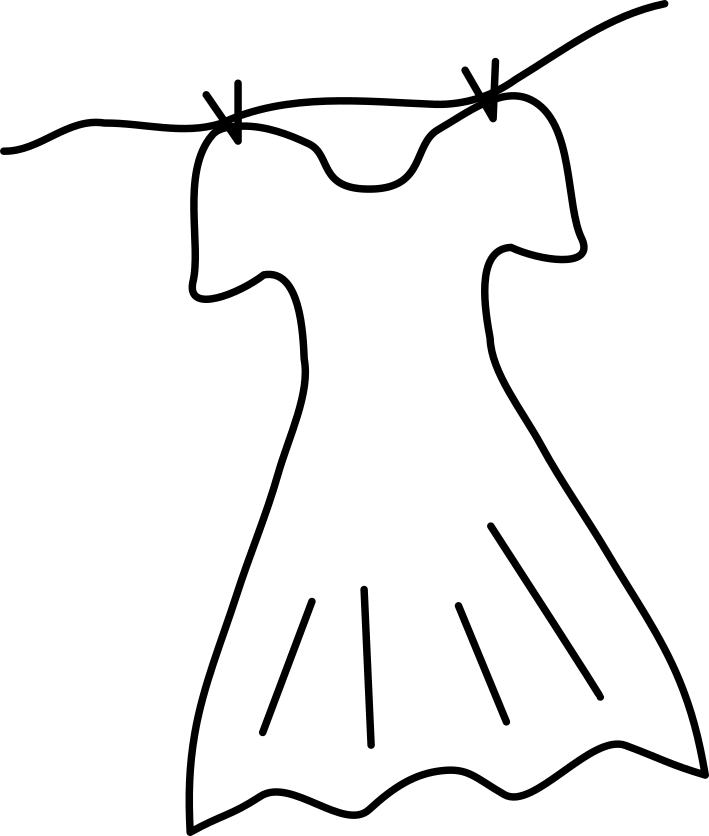
\includegraphics[scale=0.3]{i09}}
\end{figure}
\end{SBSection*}
\end{song}

\begin{song}{Вожатым быть нелегко}{}{~}{Лагерные}{}{}

\Ch{Am}{Вож}атым быть нелегко\par
И не любому дано.\par
Но дети сделают вам\par
Умней и лучше подчас.\\

\Ch{A}{П}лан\Ch{m}{ер}ка…\par
А я давно хочу уж спать!
Зар\Ch{F}{я}дка…\par
А мне не хочется вставать!\par
Уж \Ch{Dm}{пол}ночь…\par
А надо мне опять рюхать, рюх\Ch{F}{а}ть, рюхать, РЮХ\Ch{E}{А}ТЬ!\\

Припев:\\

\tt\Ch{Am}{Ты} устал и голос севший,\par 
\tt\Ch{F}{И} в вожатской надоевшей\par
\tt\Ch{Dm}{Шеп}чешь только строки эти:\par
\tt\Ch{F}{“Н}ам всего важне\Ch{E}{е} дети…”\\
\ttПусть зарплату нам не платят,\par
\ttНам улыбок детских хватит!\par
\ttНам всего важнее дети:\par
\ttСаши, Маши, Даши, Пети!\\


Нигде на этой земле\par
Нет друга ближе тебе.\par
Напарник рядом всегда,\par
Пусть радость или беда.\\

\newpage

Напарник…\par
Двадцать один день подряд!\par
Мы вместе…\par
Воспитывали ребят!\par
И души…\par
Вложили в наш отряд, отряд, отряд, ОТРЯД!\\

Припев.\\

И вроде все говорят:\par
“У вас чудесный отряд!”\par
Но только им не понять,\par
Как ночью хочется спать.\\

Вожатый…\par
Ты знаешь -- это судьба!\par
Проблемы…\par
Так это всё ерунда!\par
Отряд наш…\par
Ты будешь помнить всегда, всегда, всегда, ВСЕГДА!\\

Припев.\\

\begin{SBSection*}
\begin{figure}[b!]
\center{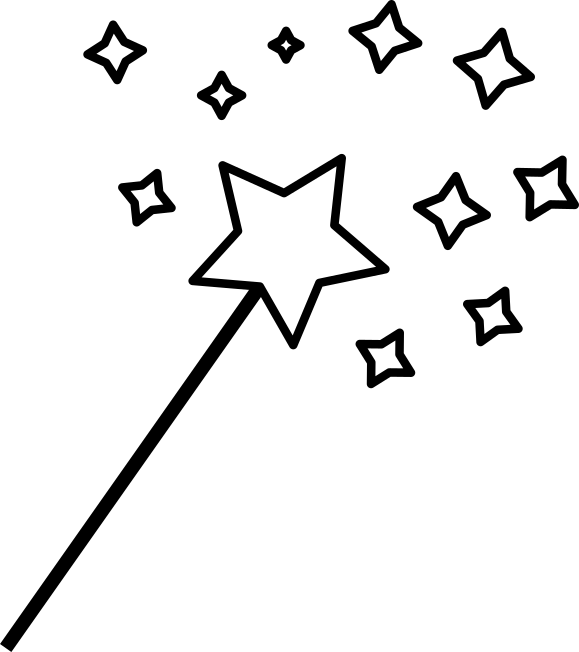
\includegraphics[scale=0.3]{i10}}
\end{figure}
\end{SBSection*}

\end{song}


\begin{song}{Пока.Целую.Снишься}{}{Торба-на-Круче}{Торба-на-Круче}{}{}

\Ch{Em}{Пос}ледняя дверь второго вагона,\par
\Ch{C}{К}ак страшно в метро не встретить тебя.\par
\Ch{Am}{Ост}алась минута до нового года, \par
\Ch{B7}{Нов}ого дня. \par
\Ch{G}{О}тсчёт идёт с момента встречи,\par 
\Ch{D}{В}едь больше ничего не лечит, \par
\Ch{Em}{Бол}ьше ничего не важно.\par
\Ch{Am}{Для} \Ch{B7}{мен}я...\\

Припев:\\
\tt\Ch{Am}{Чер}ез минуту ты уйдёшь \par
\tt\Ch{Cmaj7}{И в пе}реходах растворишься.\par 
\tt\Ch{Am}{По} Невскому гуляет дождь,\par
\ttПо \Ch{C}{Н}евскому гуляет дождь,\par 
\tt\Ch{Am}{И }в\Ch{B7}{сё}... \par
\tt\Ch{Em}{Пок}а. Целую. Снишься\Ch{C}{..}\Ch{Am}{. С}\Ch{B7}{ниш}ься... (x2)\\

\Ch{G}{О}т этих правил я болею, \Ch{D}{кр}угом голова. \par
Кто так \Ch{Em}{при}думал? \Ch{Am}{Всё} кругом, и \Ch{D}{кр}угом\par
\Ch{G}{Т}воего общенья я не \Ch{D}{пр}инят, ты права. \par
Но в тыщу \Ch{Am}{раз} важней - мы \Ch{B7}{при}няты друг другом. \\

\Ch{Am}{Чер}ез минуту ты уйдёшь \par
\Ch{Cmaj7}{И в пе}реходах растворишься.\par 
\Ch{Am}{По} Невскому гуляет дождь,\par
По \Ch{C}{Н}евскому гуляет дождь,\\

\Ch{F}{Ф}изика и химия прои\Ch{Em}{схо}дят между нами, \par
Только \Ch{Am}{сол}нце ниже, \Ch{B7}{веч}ер ближе. \par
\Ch{F}{В}ремя пролетело быстрой\Ch{Em}{ пт}ицей над волнами.\par 
Я ле\Ch{Am}{чу }фанерой над Пар\Ch{B7}{иже}м. \\

Припев:\\

\Ch{Am}{Чер}ез минуту ты уйдёшь \par
\Ch{Cmaj7}{И в пе}реходах растворишься.\par 
По \Ch{Am}{Нев}скому гуляет дож\Ch{Dm}{дь,}\par
П\Ch{Dm}{о П}итеру рыдает дождь.\par 
Я п\Ch{Em}{огу}ляю вместе с ним\Ch{B7}{ по}ка... \par
\Ch{Em}{Пок}а. Целую. Снишься\Ch{C}{..}\Ch{Am}{. С}\Ch{B7}{ниш}ься... (x2)\\

\end{song}


\begin{song}{Друг}{}{Торба-на-Круче}{Торба-на-Круче}{}{}
\noindentПерес\Ch{C}{та}л, и сн\Ch{B7}{ов}а сыпет сне\Ch{Em}{г }\par 
\noindentДля т\Ch{C}{е}бя и д\Ch{B7}{ля }меня, для в\Ch{Em}{сех}\par 
\noindentКроме вс\Ch{Am}{ех }песков пустыни, не узн\Ch{B7}{ать} им его имя\par
\noindentИм сгор\Ch{G}{ат}ь под солнцем злющим, обжиг\Ch{C}{аю}щим, плюющим\par
\noindentА над н\Ch{Am}{ами} злые тучи, холода\Ch{B7}{ вс}е круче, круче\par
\noindentИ у\Ch{Em}{же }как две недели прогноз рад\Ch{C}{ио} и теле\par
\noindentВ самом д\Ch{Am}{еле}...\par
\noindent\Ch{B7}{Зде}сь снова сыпет снег\Ch{Em}{   } \\

\noindentДля т\Ch{C}{еб}я и д\Ch{B7}{ля }меня, для в\Ch{Em}{сех} \par
\noindentЛишь в \Ch{Am}{кос}мическом пространстве, в\Ch{B7}{ че}рном звездном \noindentпостоянстве\par
\noindentГде нет\Ch{G}{ с}нега и метели, космонавты про\Ch{C}{ле}тели.\par
\noindentА у нас \Ch{Am}{как} две недели не вылази\Ch{B7}{м  }из постели\par
\noindentПоце\Ch{Em}{луя}ми на теле торопить весну \Ch{C}{х}отели \par
\noindentВ самом д\Ch{Am}{еле}...\par
\noindent\Ch{B7}{Зде}сь снова сыпет снег\Ch{Em}{   } \\

\noindentДля т\Ch{C}{еб}я и д\Ch{B7}{ля }меня, для в\Ch{Em}{сех} \par
\noindentТолько т\Ch{Am}{от, }кто самый нужный, сам\Ch{B7}{ый} северный и южный \par
\noindentСамый \Ch{G}{ищ}ущий, пропащий, самый друг м\Ch{C}{ой} настоящий \par
\noindentНе увиди\Ch{Am}{т б}ольше снега, он вчера \Ch{B7}{уш}ел на небо \par
\noindentТам \Ch{Em}{влю}бился и остался, вездеход \Ch{C}{е}го сломался\par 
\noindentСнег то ш\Ch{Am}{ел,} то\Ch{B7}{ пр}екращался, бился в \Ch{Em}{окн}а, разбивался \par
\noindentОн т\Ch{Em}{о п}лакал, то смеялся, улыбался\Ch{C}{, }улыбался \par
\noindentПопрощалс\Ch{Am}{я..}. \par
\noindentИ \Ch{B7}{сно}ва снег пош\Ch{Em}{ел.} \\

\noindentИзмен\Ch{Am}{илс}я м\Ch{D}{и}р, и хорошо\Ch{G}{  } \par
\noindentПрежний м\Ch{C}{и}р был слишком грязным, злым, ту\Ch{Am}{пым} и однообразным \par
\noindentЛицем\Ch{G}{е}рным и циничным, слишком серым и двуличным \par
\noindentА теп\Ch{Am}{ерь} грязь незаметна, мир стал белы\Ch{B7}{й, }мир стал светлый \par
\noindentТолько н\Ch{Em}{афи}г он мне сдался, лучше б друг\Ch{C}{ с}о мной остался \par
\noindentПотер\Ch{Am}{ялс}я я.\Ch{B7}{..} \par
\noindentПрекратил\Ch{Am}{ся }бег..\Ch{B7}{. }\par
\noindentПерес\Ch{C}{та}л, и сн\Ch{B7}{ов}а сыпет сне\Ch{Em}{г } x3 \\

\end{song}


\begin{song}{Мы никогда не умрём}{}{Зимовье зверей}{Зимовье зверей}{}{}

\Ch{Dm}{Мы} сегодня вс\Ch{B}{та}ли рано,вс\Ch{C}{та}ли затем\Ch{Dm}{но}.\par
Люди били в барабаны, выли матерно.\par
То ли общая тревога, то ли празднество...\par
Нам с тобою, слава богу, то без разницы.\\

\Ch{A}{}Когда мы вместе, когда мы пое-\Ch{B}{ем},\par
Такое чувство,\Ch{C}{}что мы никогда не умрем!\\

Дует ветер ледяной в нашу сторону,\par
И кричат над головой птицы-вороны.\par
Отчего же, отвечай, нам так весело?\par
Просто песня ту печаль перевесила!\\

Когда мы вместе, когда мы поем,\par
Такое чувство, что мы никогда не умрем!\\

Припев 1:\par
\tt\Ch{Dm}{}Это \Ch{Gm}{бо}льше, чем \Ch{Dm}{я}, это \Ch{Gm}{бо}льше, чем \Ch{Dm}{ты},\par
\ttЭто \Ch{Bm}{ве}чной сво\Ch{F}{бо}ды дур\Ch{A}{ма}нящий \Ch{Dm}{вдо}х!\par
\ttЭто наша любовь, это наши мечты,\par
\ttЭто с неба тебе улыбается бог!\\

\newpage

У меня сейчас внутри бочка пороху,\par
Только спичку поднеси — будет шороху!\par
А башка моя сама в петлю просится —\par
То, что сводит нас с ума, то и по сердцу!\\

Когда мы вместе, когда мы поем,\par
Такое чувство, что мы никогда не умрем!\\

Припев 1\par
Припев 2:\par
\ttЭто больше, чем я, это больше, чем ты,\par
\ttЭто теплое солнце и ночью, и днем!\par
\ttЭто наша любовь, это наши мечты,\par
\ttИ поэтому мы никогда не умрем!\\

Когда мы вместе, когда мы поем,\par
Такое чувство... Такое чувство!\\

Припев 1\par
Припев 2\\
\begin{SBSection*}
\begin{figure}[b!]
\center{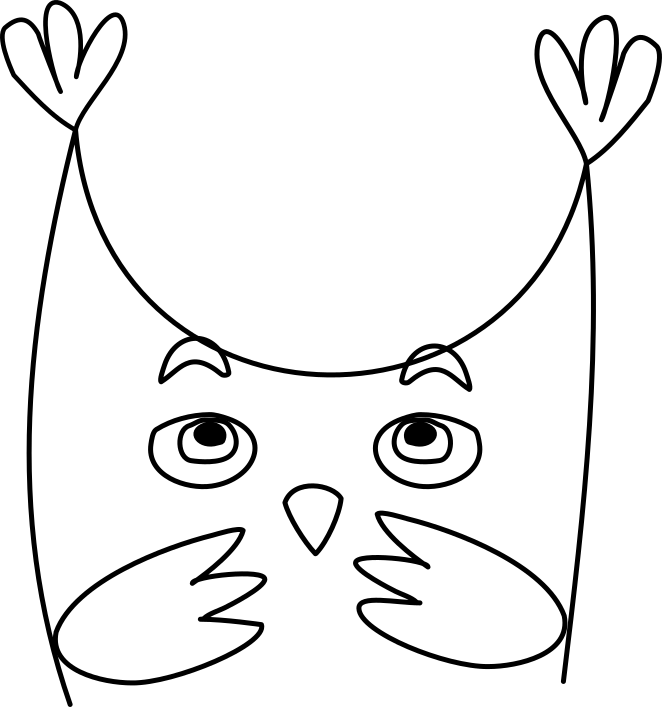
\includegraphics[scale=0.3]{i15}}
\end{figure}
\end{SBSection*}
\end{song}

\begin{song}{Впереди!}{}{~}{Сказочные}{}{}

\Ch{G}{Ру}ку мне дай на сере\Ch{Am}{ди}не пути,\par
\Ch{D7}{Ру}ку мне дай, нам ещё \Ch{G}{до}лго ид\Ch{D}{ти}!\par
\Ch{G}{Пу}сть на пути мы иног\Ch{Am}{да} устаём,\par
\Ch{D7}{Всё} же идти легче со “\Ch{G}{Ска}зкой” вдво\Ch{D}{ём}.\\ 

Припев:\\
\ttВпере\Ch{G}{ди} сотни ребят!\par
\ttВпере\Ch{Em}{ди} зори горят!\par
\ttЖёлтый \Ch{Am}{галс}тук у нас на груди!\par
\ttВпере\Ch{D7}{ди}…\par
\ttВпереди сотни ребят!\par
\ttВпереди у нас зори горят!\par
\ttЖёлтый галстук у нас на груди!\par
\ttВпереди! Жизнь впереди!\\

Мир так велик, и не кончается путь.\par
Если ты плачешь - надо слезинку смахнуть.\par
Если устал - рядом есть друга плечо,\par
Если замёрз - в сердце моём горячо.\\

\newpage

Припев:\\
\ttВедь у нас сотни ребят!\par
\ttВедь у нас зори горят!\par
\ttЖёлтый галстук у нас на груди!\par
\ttВпереди…\par
\ttВпереди сотни ребят!\par
\ttВпереди у нас зори горят!\par
\ttЖёлтый галстук у нас на груди!\par
\ttВпереди! Жизнь впереди!\\

Ты стал взрослей. в сказки не веришь порой,\par
И у костра реже сидим мы с тобой.\par
Яркий огонь может погаснуть уже,\par
Но навсегда светлые искры в душе.\\

Припев:\\
\ttНавсегда сотни ребят!\par
\ttНавсегда у нас зори горят!\par
\ttЖёлтый галстук у нас на груди!\par
\ttВпереди…\par
\ttВпереди сотни ребят!\par
\ttВпереди у нас зори горят!\par
\ttЖёлтый галстук у нас на груди!\par
\ttВпереди! Жизнь впереди!\\

\end{song}



\begin{song}{Муха}{}{Н. Олейников}{Н. Олейников}{}{}

Вступление: Am Hm5-/7 E\\

Я м\Ch{Am}{уху} без\Ch{E}{у}мно люб\Ch{Am}{ил .}  \Ch{Hm5-/7}{} \Ch{E}{} \par 
Давн\Ch{Am}{о эт}о было, друз\Ch{Dm}{ья,} \Ch{Dm7+}{} \Ch{Dm7}{} \Ch{Dm6}{}\par
Ког\Ch{Dm}{да е}щё м\Ch{Dm7+}{олод} я б\Ch{Dm}{ыл,} \Ch{Dm7+}{} \Ch{Dm7}{} \Ch{Dm6}{}\par
Когд\Ch{Dm}{а ещ}ё м\Ch{Dm7+}{олод} б\Ch{Dm}{ыл} \Ch{E}{я.} \Ch{}{}\\

Кружилась она надо мной,\par
Жужжала и билась в стекло,\par
Я с ней целовался порой,\par
И время для нас незаметно текло.\\

Припев:\par
\ttМ\Ch{Am}{у-у-}уха -- белокр\Ch{Dm}{ыла}я пт\Ch{E}{и}ца, \Ch{}{}\par
\ttМ\Ch{Am}{у-у-}уха \Ch{Dm}{-- б}оевой самол\Ch{E}{е}т.\par
\ttХот\Ch{Dm}{ел я} крыл\Ch{Dm7+}{атым} род\Ch{Dm7}{итьс}я \Ch{Dm6}{}\par
Чтобы в\Ch{Dm}{мест}е с то\Ch{Dm7+}{бой ус}т\Ch{Dm}{рем}\Ch{E}{и}ться в пол\Ch{E7}{ет.}\\

Но я уже больше не тот\par
И нет моей мухи давно\par
Она не жужжит не поет,\par
Она не стучится в окно,\\

Забытые чувства в груди,\par
И сердце гложет змея,\par
И нет ничего впереди.\par
О, Муха! О, птичка моя!\\

Припев.\\
\end{song}

\begin{song}{Романтика}{}{~}{Сказочные}{}{}

Ты\Ch{Em}{}провожала мен\Ch{Am}{я в п}орту,\par
Т\Ch{D7}{их}о катилась слез\Ch{G}{а}.\par
\Ch{Am}{Я ц}еловал твои в\Ch{Em}{ол}осы\par
\Ch{H7}{И }голубые глаз\Ch{Em}{а}.\\

Если придётся когда-нибудь\par
Мне в океане тонуть,\par
То на твою фотографию\par
Не позабуду взглянуть.\\

Руки, сведенные холодом,\par
Молча к тебе протяну\par
И навсегда успокоенный\par
Камнем отправлюсь ко дну.\\

Буду лежать я на дне морском,\par
И о тебе вспоминать,\par
Буду твоей фотографией\par
Я осьминогов пугать.\\

Всё потеряю на дне морском:\par
Сон, аппетит и покой.\par
Даже твою фотографию\par
Вырвет акула с рукой.\\

Буду лежать я на дне морской\par
Грудой холодных камней.\par
Вот, что такое романтика\par
В жизни бродячей моей.\\
\end{song}

\begin{song}{Моё сердце}{}{Сплин}{Сплин}{}{}

Мы не зн\Ch{D}{а}ли друг друга до эт\Ch{G}{о}го лета,\Ch{D}{ }\par
Мы болт\Ch{G}{а}лись по све\Ch{D}{т}у - зе\Ch{A}{м}ле и воде,\Ch{Bm}{  }\par
И соверш\Ch{D}{е}нно случайно мы взя\Ch{G}{л}и билет\Ch{D}{ы}\par
На сос\Ch{G}{е}днее крес\Ch{D}{л}о на большой\Ch{A}{ }высоте.\Ch{Bm}{  }\\

Припев:\par
\ttИ мое с\Ch{D}{е}рдце \Ch{G}{о}станови\Ch{D}{л}ось,\par
\ttМо\Ch{D}{е} сердце з\Ch{A}{а}мерло.\Ch{Bm}{  }\par
\ttИ мое с\Ch{D}{е}рдце \Ch{G}{о}станови\Ch{D}{л}ось,\par
\ttМо\Ch{D}{е} сердце з\Ch{A}{а}мерло.\Ch{Bm}{  }\\

Проигрыш: D G D D A Bm x2\\

И ровно тысячу лет мы просыпаемся вместе,\par
Даже если уснули в разных местах.\par
Мы идём ставить кофе под Элвиса Пресли,\par
Кофе сбежал под Propeller Heads. Ах!\\

Припев:\\

Проигрыш: D G D D A Bm x2\\

И, может быть, ты не стала звездой в Голливуде,\par
Не выходишь на подиум в нижнем белье.\par
У тебя не берут автографы люди,\par
И поёшь ты чуть тише, чем Монсерат Кабалье.\\

\newpage

Но так и я, слава Богу, не Рики, не Мартин,\par
Не выдвигался на Оскар, французам не забивал.\par
Моим именем не назван город на карте, \par
Но задёрнуты шторы и разложен диван.\\

Припев\\

Проигрыш: D G D D A Bm x2\\

Я наяву \Ch{D}{в}ижу то, что многим\Ch{G}{ }даже не\Ch{D}{ }снилось,\par 
Не являл\Ch{G}{о}сь под кай\Ch{D}{ф}ом, н\Ch{A}{е} стучалось \Ch{Bm}{в} стекло.\par
Моё серд\Ch{D}{ц}е остановилось, отд\Ch{G}{ы}шалось\Ch{D}{ }немного\par
И снова\Ch{G}{ }по\Ch{D}{ш}л\Ch{A}{о}. \Ch{Bm}{  }\\

Припев:\par
\ttИ мое сердце остановилось,\par
\ttМое сердце замерло.\par
\ttИ мое сердце Hasta La Vista,\par
\ttМое сердце замерло.\\

\begin{SBSection*}
\begin{figure}[b!]
\center{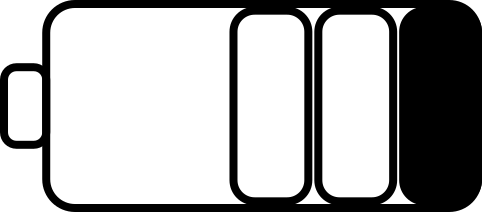
\includegraphics[scale=0.3]{i11}}
\end{figure}
\end{SBSection*}
\end{song}

\begin{song}{Новые люди}{}{Сплин}{Сплин}{}{}

Вступление: Dm G Dm G\\

За\Ch{Am}{мер} троллейбус в троллейбусн\Ch{G}{о}м парке,\par
Перепут\Ch{C}{а}л механик провода по \Ch{Am}{за}парке,\par
Вы\Ch{Dm}{клю}чив лампочки в сорок электросвечей\Ch{G}{,}\par
Л\Ch{Dm}{юди} ночами делают новых людей\Ch{G}{.}\\

Та\Ch{Am}{кие} тонкие стены из цветного\Ch{G}{ }картона\par
В светл\Ch{C}{о}-серых дворцах из сте\Ch{Am}{кла} и бетона,\par
Д\Ch{Dm}{ове}ряя всему, что плетут из дневных новост\Ch{G}{е}й,\par
Л\Ch{Dm}{юди} ночами делают новых люде\Ch{G}{й}.\\

Припев:\par
\ttЛ\Ch{C}{ю}ди кричат, задыхаясь/Ch{Am}{ от} счастья,\par
\ttИ сто\Ch{C}{н}ут так сладко и дышат\Ch{Am}{ та}к часто, что\par
\ttХо\Ch{Dm}{чет}ся двигаться с каждой секундой быстрей.  \Ch{G}{  }\par
\ttД\Ch{Dm}{ела}я, делая, делая новых людей. \Ch{G}{  }\\

Проигрыш:  Am G C Am Dm G\\


\newpage

Думают люди в Ленинграде и Риме,\par
Что смерть - это то, что бывает с другими,\par 
Что жизнь так и будет крутить и крутить колесо.\par
Слышишь, на кухне замерли стрелки часов.\\

Но ничего-ничего - погрустит и забудет,\par
Через время появятся новые люди.\par
Едут троллейбусы без габаритных огней.\par
Люди ночами делают новых людей.\\

Припев:\par
\ttЛюди кричат, задыхаясь от счастья,\par
\ttИ стонут так сладко и дышат так часто, что\par
\ttХочется двигаться с каждой секундой быстрей.\par
\ttДелая, делая, делая новых людей.\\

Лю\Ch{Dm}{дям} так нравится делать новых люде\Ch{G}{й}.\\

Проигрыш:  Am G C Am Dm G\\


\begin{SBSection*}
\begin{figure}[b!]
\center{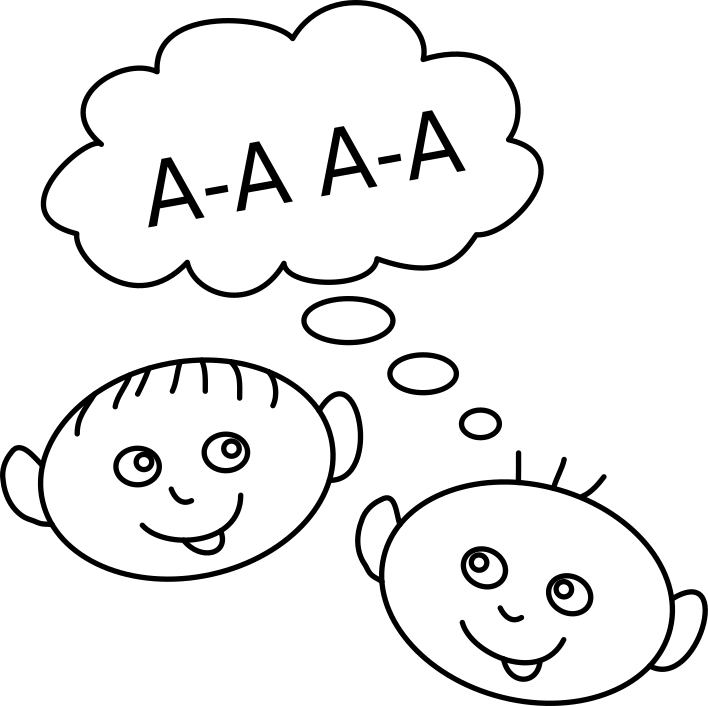
\includegraphics[scale=0.3]{i12}}
\end{figure}
\end{SBSection*}
\end{song}


\begin{song}{Выхода нет}{}{Сплин}{Сплин}{}{}

\Ch{Em}{  }Сколько лет прошл\Ch{C}{о}, всё о то\Ch{G}{м} же гудят провода,\par
\Ch{C}{  }Всё т\Ch{G}{о}го же ждут самолё\Ch{D}{т}ы.\par
\Ch{Em}{  }Девочка с гла\Ch{C}{з}ами из са\Ch{G}{м}ого синего льда\par
\Ch{C}{  }Тает п\Ch{G}{о}д огнём пулемё\Ch{D}{т}а.\par
\Ch{Em}{  }Должен же \Ch{C}{р}астаять хоть кто-\Ch{G}{т}о.\\

Припев:\par
\ttСкоро рассв\Ch{Em}{ет,} выхода не\Ch{C}{т},\par
\ttКлюч поверн\Ch{G}{и} и полет\Ch{D}{е}ли.\par
\ttНужно впи\Ch{Em}{сат}ь в чью-то тетра\Ch{C}{д}ь\par
\ttКровью, как в \Ch{G}{м}етрополит\Ch{D}{е}не,\par
\ttВыхода \Ch{C}{н}ет,\Ch{D}{  } Выхода нет. \\

Где-то мы расстались, не помню в каких городах,\par
Словно это было в похмелье.\par
Через мои песни идут, идут поезда,\par
Исчезая в тёмном тоннеле.\par
Лишь бы мы проснулись в одной постели.\\

Припев\\

Сколько лет пройдёт, всё о том же гудеть проводам,\par
Всё того же ждать самолётам.\par
Девочка с глазами из самого синего льда\par
Тает под огнём пулемёта.\par
Лишь бы мы проснулись с тобой в одной постели.\\

Припев
\end{song}

\begin{song}{Мы пройдём сквозь земной простор ССО “Славяне”}{}{~}{Отрядные}{}{}

Мы прой\Ch{Em}{дём} сквозь земной простор\par
По рав\Ch{Am}{нин}ам и пере\Ch{H7}{ва}лам,\par
По вер\Ch{Em}{шин}ам огромных гор,\par
Сквозь зем\Ch{Am}{ной} простор небы\Ch{D}{в}алый.\\

Припев:\par
\ttВедь не\Ch{G}{д}аром вста\Ch{D}{ё}т за\Ch{G}{р}я,\par
\ttНебо\Ch{C}{с}вод от за\Ch{D}{р}и весь \Ch{G}{к}расный.\par
\ttТолько зн\Ch{Am}{ать} бы, что \Ch{H7}{вс}ё не \Ch{Em}{зря},\par
\ttТолько \Ch{Am}{зна}ть бы,\Ch{H7}{  }что не на\Ch{Em}{пра}сно.\par
\ttТолько \Ch{C}{з}нать бы, что \Ch{D}{в}сё не \Ch{G}{з}ря,\par
\ttТолько \Ch{Am}{зна}ть бы,\Ch{H7}{  }что не на\Ch{Em}{пра}сно.\\

Не бывает на свете чудес,\par
Всё мы сделаем своими руками.\par
Города, что растут до небес,\par
Никогда не построятся сами.\\

Припев\\

Мы пройдём сквозь земной простор,\par
Будет много нас и будем мы вместе!\par
Ну, а те, кто придут потом,\par
Пусть подхватят вот эту песню.\\

Припев\\

\end{song}

\begin{song}{Гимн ССО ЛЭТИ}{}{}{Отрядные}{}{}

Вступление: Em A F G H (2р)\\

\Ch{Em}{Все}! Окончен по\Ch{G}{с}ледний эк\Ch{A}{з}амен.\par
\Ch{Em}{Вно}вь реет от\Ch{G}{р}ядное \Ch{A}{з}намя.\par
\Ch{C}{В}новь дороги зо\Ch{G}{в}ут нас туда,\par
Где \Ch{F}{с}ильные руки нуж\Ch{H7}{ны}.\par
Пусть ищут другие славу,\par
Нам всё по плечу и по нраву.\par
Дарит нам золотые лучи \par
Утро родной страны.\\

Припев: \par
\tt\Ch{Em}{Нам} не \Ch{Am}{зна}ть покоя,\par
\tt\Ch{D}{Ж}изнь не\Ch{G}{м}ного стоит,\par
\tt\Ch{C}{Е}сли \Ch{F}{т}ы не строил,\par
\tt\Ch{F#}{А }сидел в теп\Ch{H}{л}е, зараза!\par
\ttПеть и делать дело,\par
\ttЧтоб спина болела,\par
\ttЧтобы вновь хотелось, вновь хотелось\par
\tt\Ch{F#}{Жи}ть на \Ch{H}{э}той зем\Ch{Em}{ле.}\\

\newpage

В путь и все сомненья отбросим,\par
Мы лёгкой работы не просим.\par
Первый дом, как большая любовь,\par
Вечно помнится нам.\par
Мы втрое сильней, если надо,\par
Нам счастье людское награда,\par
На мозолистых наших руках\par
Солнце будущих дней.\\

Припев\\

Пусть нас караулят дипломы,\par
Но нам не сидеть больше дома,\par
Манит нас в неизвестную даль\par
Слово простое - «отряд».\par
Пусть все это трудно и сложно,\par
Мы всюду придем и поможем,\par
Чтобы помнили люди всегда\par
Нас, мат-мех, ЛГУ.\\

Припев\\

\begin{SBSection*}
\begin{figure}[b!]
\center{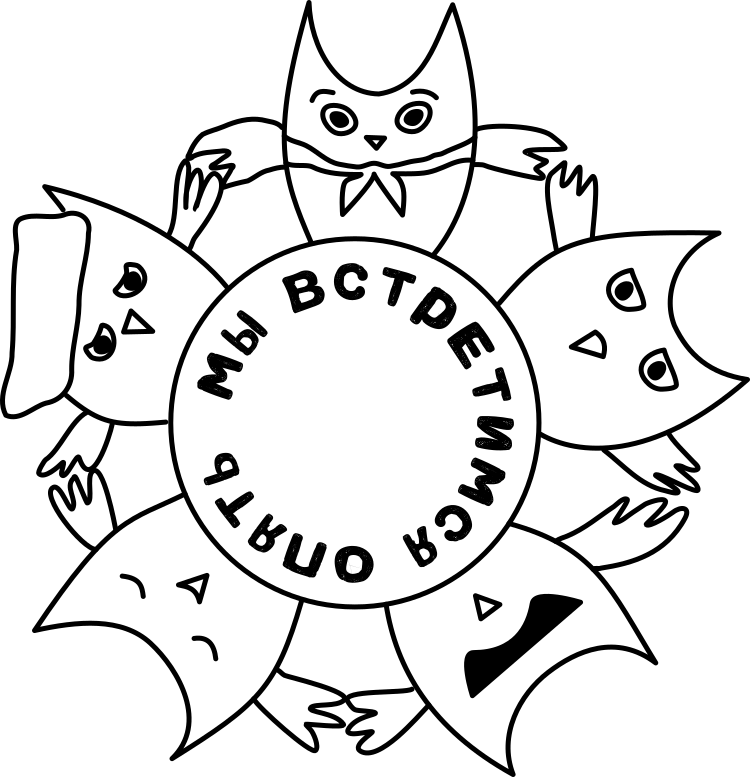
\includegraphics[scale=0.3]{i13}}
\end{figure}
\end{SBSection*}

\end{song}

\begin{song}{Между небом и потолком}{}{Д.Поляков, А.Тимофеев}{Д.Поляков, А.Тимофеев}{}{}

\tt\Ch{D}{  }Я маленький мальчик\par
\tt\Ch{G}{  }С мечтами о мире,\par
\tt\Ch{Hm}{  }Вечно счастливый\par
\ttИ \Ch{A}{б}есконечно яркий.\par
\ttВ зеленой рубашке\par
\ttВаляюсь на крыше,\par
\ttИ мысли о вечном\par
\ttВзлетают все выше.\\

\ttПрипев:\par
\tt\ttМежду \Ch{G}{н}ебом и \Ch{A}{п}отолком\par
\tt\ttМои \Ch{D}{м}ысли, как листья,\par
\tt\ttЛетают по ветру и \Ch{Hm}{им }легко.\par
\tt\ttМежду небом и потолком,\par
\tt\ttНарисую созвездие\par
\tt\ttИ дам ему вечное имя - любовь.\par
\tt\ttМежду \Ch{G}{н}ебом и \Ch{A}{п}отолком. \Ch{D}{  }\\

\ttЯ маленький мальчик,\par
\ttНо вырасту скоро. \par
\ttСтану высоким\par
\ttИ жутко остроумным.\par
\ttЯ буду стараться,\par
\ttЧтоб выросли крылья,\par
\ttИ, может быть, скоро\par
\ttЯ стану всесильным.\\

\ttПрипев\\

Я маленький мальчик\par
И скоро состарюсь,\par
Но мысли о вечном \par
Меня не оставят.\par
По-прежнему бодрый,\par
В ребячьей одежде \par
Залезу на крышу\par
И вспомню как прежде.\\

Припев\\

\begin{SBSection*}
\begin{figure}[b!]
\center{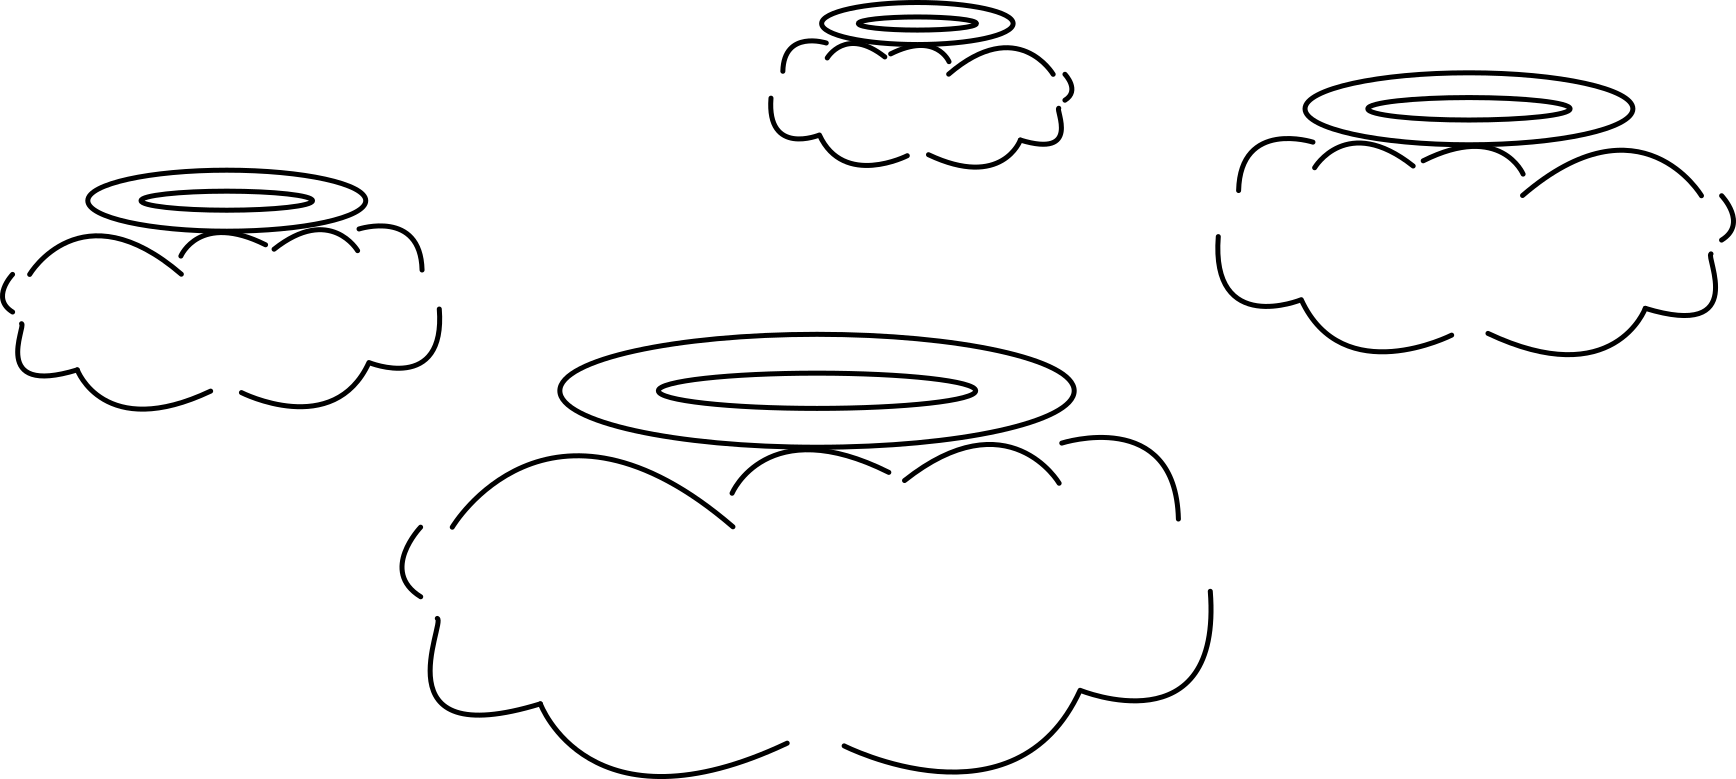
\includegraphics[scale=0.2]{i16}}
\end{figure}
\end{SBSection*}
\end{song}

\begin{song}{Оркестр}{}{~}{Лагерные}{}{}

\Ch{C}{Мы} все знакомы очень да\Ch{Am}{вно},\par
Х\Ch{Dm}{оть} и не часто, но всё-таки случал\Ch{G}{ос}ь.\par
С\Ch{C}{мо}трели мы в \Ch{Am}{одн}о окно,\par
И\Ch{Dm}{ ин}огда даже получало\Ch{G}{сь}.\\

Припев:\\
\ttН\Ch{Dm}{е з}аб\Ch{G}{ыв}айте, что м\Ch{C}{ы }все вмес\Ch{Am}{те!}\par
\ttН\Ch{Dm}{е з}абы\Ch{G}{ва}йте, что м\Ch{C}{ы }друзья!  \Ch{Am}{  }\par
\ttН\Ch{Am}{е з}абы\Ch{G}{ва}йте, что м\Ch{C}{ы }оркестр! \Ch{Am}{   }\par
\ttН\Ch{Dm}{е з}абыва\Ch{G}{й,} что ты - это \Ch{C}{я!}\\

Мы все взрослеем, это не изменить…\par
Уходит детство в никуда.\par
У нас у всех тревоги свои\par
Но мы же вместе навсегда.\\

Припев\\

Не разойтись нам никогда\par
На небе встретимся мы снова\par.
Ведь вы же все мои друзья - \par
У нас у всех одна дорога.\\

Припев\\
\end{song}

\begin{song}{Ты, да я, да мы с тобой}{}{~}{Лагерные}{}{}
Последние 3 строчки каждого куплета, поются 2 раза.\\

\Ch{Am}{Ты,} да я, да мы с тобой!\par
\Ch{Am}{Ты,} да я, да мы с тобой!\par
\Ch{A7}{Здо}рово, когда на свете есть друзь\Ch{Dm}{я. }\par
Если б жили все в оди\Ch{G}{но}чку,\par
\Ch{C}{То} б уже давно на к\Ch{F}{ус}очки\par
\Ch{Dm}{Раз}валилась бы, н\Ch{E}{ав}ерное, земл\Ch{A7}{я. }\\

Ты, да я, да мы с тобой!\par
Ты, да я, да мы с тобой!\par
Землю обогнем, потом махнем на Марс.\par
Может, у оранжевой речки\par
Там уже грустят человечки,\par
От того, что слишком долго нету нас.\\

Ты, да я, да мы с тобой!\par
Ты, да я, да мы с тобой!\par
Нас не разлучит ничто и никогда.\par
Даже если мы расстаемся,\par
Дружба все равно остается.\par
Дружба остается с нами навсегда.\par
\end{song}

\begin{song}{Дыхание}{}{Наутилус Помпилиус}{Наутилус Помпилиус}{}{}

\Ch{D}{  }Я просыпаюсь\Ch{A}{ в} холодном поту\Ch{Bm}{,  }\par
  Я просыпаюсь\Ch{F#}{ в }кошмарном бред\Ch{G}{у,}\par
  Как будто дом наш\Ch{D}{ з}алило водо\Ch{Em}{й, }\par
  И что в живых остались то\Ch{Bm}{льк}о мы с тобой.\par
\Ch{D}{  }И что над нами\Ch{A}{ к}илометры вод\Ch{Bm}{ы, }\par
  И что над нами\Ch{F#}{ б}ьют хвостами киты\Ch{G}{, }\par
  И кислорода\Ch{D}{ н}е хватит на двоих,\par
\Ch{Em}{  Я} лежу в темноте\Ch{Bm}{.  }\\

Припев:\par
\tt\Ch{Bm}{Слу}шая наше дых\Ch{A}{ан}ие,\par
\ttЯ сл\Ch{Bm}{уша}ю наше дых\Ch{G}{ан}ие.\par
\ttЯ р\Ch{Bm}{ань}ше и не думал, что у на\Ch{A}{с }\par
\ttНа дво\Ch{Bm}{их }с тобой одно лишь дыха\Ch{G}{ни}е, дыха\Ch{Bm}{ние}.\\

И я пытаюсь разучиться дышать,\par
Чтоб тебе хоть на минуту отдать\par
Того газа, что не умели ценить,\par
А ты спишь и не знаешь.\par
Что над нами километры воды,\par
И что над нами бьют хвостами киты,\par
И кислорода не хватит на двоих,\par
Я лежу в темноте.\\

\ttПрипев\\
\end{song}

\begin{song}{Все расстояния}{}{~}{Лагерные}{}{}

\Ch{Am}{Все} расстоянья когда-нибудь в круг замы\Ch{E}{ка}ются,\par
\Ch{E}{Все} из разлук обязательно \Ch{E7}{встре}чей кон\Ch{Am}{ча}ются;\par
Должны про\Ch{Dm}{плыть} вокруг Зем\Ch{G}{ли,}\par
Вернуться в \Ch{C}{га}вань кораб\Ch{F}{ли,}\par   
Все поез\Ch{Dm}{да} в свои вер\Ch{E}{нуть}ся горо\Ch{Am}{да.}\par
 
Шумный вокзал то встречает друзей , то прощается,\par
Мы расстаемся, но снова назад возвращаемся -\par
Чтоб снова встать в огромный круг,\par
И снова знать, что рядом друг ,\par
И песни петь, чтоб больше не было разлук.\par
 
Все расстоянья когда-нибудь в круг замыкаются,\par
Все из разлук обязательно встречей кончаются;\par
И через год, и через пять,\par
Мы с вами встретимся опять,\par
Ничто не сможет нашей дружбе помешать.\par
\begin{SBSection*}
\begin{figure}[b!]
\center{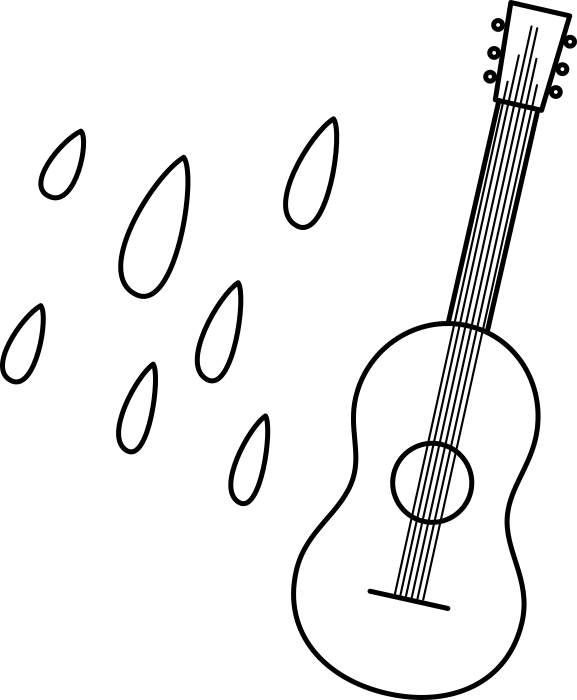
\includegraphics[scale=0.3]{i14}}
\end{figure}
\end{SBSection*}
\end{song}

\begin{song}{Районы-кварталы}{}{Звери}{Звери}{}{}

Вступление: Am Dm E7 Am F Dm E7 Am\\

\Ch{Am}{Бол}ьше нече\Ch{Dm}{го }ловить - \Ch{E7}{все}, что надо, \Ch{Am}{я п}оймал.\par
Надо сразу уходить, чтоб никто не привыкал.\par
\Ch{Am}{Ярк}о-жёлты\Ch{Dm}{е о}чки, \Ch{G}{д}ва сердечка \Ch{C}{н}а брелке,\par
\Ch{F}{Р}азвеселы\Ch{Dm}{е з}рачки, \Ch{E7}{тв}ое имя на руке.\\

Припев (2р)\par
\ttРай\Ch{Am}{оны}, квар\Ch{Dm}{тал}ы, жи\Ch{E7}{лы}е мас\Ch{Am}{сив}ы,\par
\tt\Ch{F}{Я} ухо\Ch{Dm}{жу,} ухо\Ch{E7}{жу} кра\Ch{Am}{сив}о.\\

У тебя все будет класс, будут ближе облака.\par
Я хочу, как в первый раз, и поэтому пока.\par
Ярко-жёлтые очки, два сердечка на брелке,\par
Развеселые зрачки, я шагаю налегке.\\

Припев (2р)\\

Вот и все, никто не ждет, и никто не в дураках,\par
Кто-то любит, кто-то врет и летает в облаках.\par
Ярко-жёлтые очки, два сердечка на брелке,\par
Развеселые зрачки, я шагаю налегке.\\

Припев(2р)\\
\end{song}

\mainmatter

\renewcommand{\footrulewidth}{0.0pt}
\renewcommand{\item}{\par\hangindent=40pt}
\renewcommand{\subitem}{\par\hangindent=40pt \hspace*{20pt}}
\renewcommand{\subsubitem}{\par\hangindent=40pt \hspace*{30pt}}

\newpage
\raggedright%\documentclass[a5paper,11pt]{book}
%\usepackage{fancyhdr}
%\usepackage[chordbk]{songbook}
%
%\usepackage[T2A]{fontenc}
%\usepackage[utf8]{inputenc}
%\usepackage[russian]{babel}
%
%\title{A Church Songbook}
%\author{}
%\date{Revised:  \RevDate}
%
%\newcommand{\RelDate}{13 November'19}
%\newcommand{\RevDate}{\today}

\documentclass[11pt,a5paper]{book}
\usepackage[a5paper]{geometry}
\usepackage[chordbk]{songbook}
\usepackage[T2A]{fontenc}
\usepackage[utf8]{inputenc}
\usepackage[russian]{babel}
\usepackage{cmap} % для работы поиска кириллицы в pdf

%\usepackage{amsmath,amsthm,amssymb}
%\usepackage{mathtext}


\usepackage[pdftex]{graphicx}
\usepackage{lscape}
%\usepackage{vmargin}
\usepackage{textcomp}
\usepackage{setspace}
%\usepackage{marvosym}
\usepackage{gensymb} %%%for \micro tag
\usepackage{upgreek} %%% \upmu
\usepackage{tipa}
\usepackage{phonetic}
%\usepackage[greek,english]{babel}
\usepackage{threeparttable}
\usepackage{multirow}
\usepackage{harvard}
\usepackage{longtable}
\renewcommand{\sectionmark}[1]{\markright{#1}}
\renewcommand{\chaptermark}[1]{\markboth{#1}{}}
\addto\captionsenglish{\renewcommand{\bibname}{References}}
\usepackage{latexsym,fancyhdr}

\newcommand{\RelDate}{26 Апреля'1984}
\newcommand{\RevDate}{\today}

%%%
% C.C.L.I. license number definition; for copyright licensing info.
% One of these macros will be manually inserted into the {CpyRt}
% parameter of the {song} environment.
%
%       \CCLInumber - The actual copyright license number.  Don't
%               insert this command in the {CpyRt} parameter, use one
%               of the others.
%       \CCLIed - Indicates a song falls under our CCLI license.
%       \NotCCLIed - Indicates a song doesn't fall under our CCLI
%               license.  Public Domain songs fall into this category.
%       \PGranted - We have received specific permission from the
%               copyright holder to use this song.
%       \PPending - We are in the process of obtaining permission to
%               use this song.
%%%
\newcommand{\CCLInumber}{Your CCLI Number}
\newcommand{\CCLIed}{{\CpyRtInfoFont (CCLI \CCLInumber)}}
\newcommand{\NotCCLIed}{\relax}
\newcommand{\PGranted}{\relax}
\newcommand{\PPending}{{\CpyRtInfoFont (Permission Pending)}}

%%%
% Title page information.
%%%
\title{ Сказочный песенник}
\author{}
\date{Созданно:  \RevDate}


%%%
% Define fonts to use in the headers and footers of the songbook.
%%%
\newcommand{\LHeadFont}{\normalsize}            % = cmr12  at 12pt
\newcommand{\CHeadFont}{\normalsize\rm}         % = cmr12  at 12pt
\newcommand{\RHeadFont}{\normalsize}            % = cmr12  at 12pt
\newcommand{\LFootFont}{\scriptsize}            % = cmr8   at  8pt
\newcommand{\CFootFont}{\tiny\myTinySF}         % = cmss8  at  8pt
\newcommand{\RFootFont}{\scriptsize}            % = cmr8   at  8pt

%%%
% Turn on and define fancy page heading/footing definition.
%%%
\pagestyle{fancy}

\ifChordBk
  % It's a words & chords songbook...
%  \addtolength{\headwidth}{\marginparsep}
%  \addtolength{\headwidth}{\marginparwidth}
  \renewcommand{\headrulewidth}{0.0pt}
  \renewcommand{\footrulewidth}{0.0pt}
%  \fancyhead[LE,RO]{\LHeadFont\emph{\leftmark\/}}
%  \fancyhead[CE,CO]{\CHeadFont\thepage}
  \fancyhead[RE,LO]{~}
\else\ifOverhead
  % It's an overhead...
  \renewcommand{\footrulewidth}{0pt}
  \renewcommand{\headrulewidth}{0pt}
  \fancyhead[LE,RO]{}
  \fancyhead[CE,CO]{}
  \fancyhead[RE,LO]{}
\else\ifWordBk
  % It's a words only songbook...
  \addtolength{\headwidth}{\marginparsep}
  \addtolength{\headwidth}{\marginparwidth}
  \renewcommand{\headrulewidth}{0.0pt}
  \renewcommand{\footrulewidth}{0.0pt}
  \fancyhead[LE,RO]{\LHeadFont A Church Songbook}
  \fancyhead[CE,CO]{\CHeadFont\thepage}
  \fancyhead[RE,LO]{\RHeadFont\RelDate}
\fi\fi\fi

%\fancyfoot[LE,RO]{\LFootFont Property of The Church}
%\ifSongEject
%  \fancyfoot[CE,CO]{\CFootFont \RevDate}
%\else
%  \fancyfoot[CE,CO]{\CFootFont}
%\fi
%\fancyfoot[RE,LO]{\RFootFont Material used by permission.}

%%%
% Turn on/off index-file generation.  Uncomment the \makeindex line to
% turn index generation on;  comment it out to turn index generation
% off.
%%%
\makeTitleIndex         %% Title and First Line Index.
\makeTitleContents      %% Table of Contents.
\makeKeyIndex           %% Index of song by key.
\graphicspath{{img/}} % папка с картинками
\DeclareGraphicsExtensions{.pdf,.png,.jpg} % форматы, которые будем считать картинками

%\newenvironment{song}[7][Y]{
%% Comment markers to negate
%\if#1Y\ExcludeSongfalse\else\ExcludeSongtrue\fi% the newline.
%\ifPrintAllSongs\ExcludeSongfalse\fi
%\SongMarkboth{\relax}{\relax}
%\SBinSongEnvtrue
%\renewcommand{\SBinSongEnv}{\True}
%\ifWordsOnly
%	\setlength{\parindent}{0pt}
%\fi

%%%
% Redefine fonts from SongBook style that I don't like.
%%%
\font\myTinySF=cmss8 at 8pt
\renewcommand{\CpyRtInfoFont}{\tiny\myTinySF}


%
%\font\myTinySF=cmss8    at  8pt
%\font\myHugeSF=cmssbx10 at 25pt
%\renewcommand{\CpyRtInfoFont}{\tiny\myTinySF}
%\newcommand{\myTitleFont}{\Huge\myHugeSF}
%\newcommand{\mySubTitleFont}{\large\sf}

%%% Работа с русским языком
%\usepackage[no-math]{fontspec}      %% подготавливает загрузку шрифтов Open Type, True Type и др.
%\defaultfontfeatures{Ligatures={TeX},Renderer=Basic}  %% свойства шрифтов по умолчанию
%\setmainfont[Ligatures={TeX,Historic}]{Times New Roman} %% задаёт основной шрифт документа
%\setsansfont{Helvetica Neue}                    %% задаёт шрифт без засечек

%\newfontfamily{\allods}{AllodsWest}

\newcommand{\SBPubDomm}{~}
\renewcommand{\CpyRt}[3][Y]{%
\if#1Y\begin{center}\fi
\if\blank{#2}%
\if\blank{#3}%
{\CpyRtFont\copyright \SBUnknownTag{} \CpyRtInfoFont}%
\else
{\CpyRtFont\copyright \SBUnknownTag{} \CpyRtInfoFont #3}%
\fi%
\else%
\ifthenelse{\equal{#2}{\SBPubDomm}}
{%then
{\CpyRtFont #2 \CpyRtInfoFont #3}%
}{%else
{\CpyRtFont #2 \CpyRtInfoFont #3}%
}%fi
\fi%
\if#1Y\end{center}\fi
}


\newcommand{\SBUnknownTagg}{~}
\renewcommand{\WAndM}[2][Y]{~}
\renewcommand{\WAndM}[2][Y]{%
\if#1Y\begin{center}\fi
\if\blank{#2}%
{\SBUnknownTagg}%
\else
{~}%
\fi
\if#1Y\end{center}\fi
}

\renewcommand{\STitle}[3][Y]{%
\setcounter{SBVerseCnt}{0}%
\setcounter{SBSectionCnt}{0}%
\ifExcludeSong\relax%
	\else\keyIndex{{\protect\sbChord#3\protect\relax} -- #2}{\theSBSongCnt}\fi%
	\vspace{\SpaceAboveSTitle}%
\if#1Y\begin{center}\fi
	{}{\STitleFont\LARGE #2}%
	\ifWordsOnly\relax\else\fi%
	\if#1Y\end{center}\fi
\STitleMarkboth{#2}{\relax}%
}


%\renewenvironment{SBOpGroup}{%
%	\sbSetsbBaselineSkipAmt%
%	\bgroup%
%	\begin{list}{\hbox{}}
%	  {\setlength {\leftmargin}
%		{\HangAmt}
%		\setlength{\itemindent}
%			{-\HangAmt}
%		\setlength{\listparindent}{-\HangAmt}
%		\setlength{\topsep}{0pt}
%		\setlength{\parsep}{0pt}
%		\setlength{\labelwidth}{0pt}
%		\setlength{\labelsep}{0pt}
%		\setlength{\baselineskip} {\sbBaselineSkipAmt}
%	}%\item}
%{\end{list}%
\newcommand{\SBChorusTagg}{Припев}
\renewenvironment{SBChorus}{%
\sbSetsbBaselineSkipAmt%
\bgroup%
\SBChorusMarkright{\SBChorusTag}
\begin{list}{{\SBChorusTagFont\SBChorusTagg}}
{\setlength {\leftmargin}
{\LeftMarginSBChorus + \HangAmt}
\setlength{\itemindent}
{-\HangAmt}
\setlength{\listparindent}{-\HangAmt}
\setlength{\parsep}
{0pt}
\setlength{\baselineskip} {\sbBaselineSkipAmt}
}%
\item}
{\end{list}%
\egroup%
\SpaceAfterChorus%
}

\renewcommand{\tt}{\indent \indent}
%\renewcommand{\nt}{\noindent}


\usepackage{amsmath}

\makeArtistIndex
\makeTitleIndex         %% Title and First Line Index.
\makeTitleContents      %% Table of Contents.
\makeKeyIndex           %% Index of song by key.
%\usepackage{printallsongs}

\begin{document} 
\maketitle

\mainmatter


\begin{song}{Вожатский гимн}{}{Сказка}{Сказка}{}{}

По \Ch{Am}{ла}герю подъём, нас горн зовёт!\par
Забудь о том, что ночь была бес\Ch{C}{сон}ною\par
Смо\Ch{Dm}{чи} водою \Ch{G}{ве}ки воспа\Ch{C}{лён}\Ch{F}{ные}\par    
По\Ch{Dm}{вя}зывай свой \Ch{E}{галс}тук — и впе\Ch{Am (A7)}{рёд!}\par
Смо\Ch{Dm}{чи} водою \Ch{G}{ве}ки воспа\Ch{C}{лён}\Ch{F}{ные}\par    
По\Ch{Dm}{вя}зывай свой \Ch{E}{галс}тук — и впе\Ch{Am (A7)}{рёд!}\par

%	\begin{SBChorus*}
\ttНе\Ch{E}{про}сто воспитывать \Ch{Am}{но}вых людей,\par
\ttНу \Ch{E}{что} ж, это наша с то\Ch{Am}{бою} свя\Ch{A7}{ты}ня.\par
\ttМой \Ch{Dm}{друг}, нам до\Ch{G}{ве}рили \Ch{C}{ду}ши де\Ch{F}{тей},\par
\ttИх \Ch{Dm}{ра}достный \Ch{Am}{смех} нам на\Ch{E}{гра}да от\Ch{Am}{ны}не.\par
\ttМой \Ch{Dm}{друг}, нам до\Ch{G}{ве}рили \Ch{C}{ду}ши де\Ch{F}{тей},\par
\ttИх \Ch{Dm}{ра}достный \Ch{Am}{смех} нам на\Ch{E}{гра}да от\Ch{Am}{ны}не.\\
%\end{SBChorus*}

Отбой, засыпает детвора.\par
Взгляни на их улыбки полусонные,\par
Пускай им снятся острова зелёные,\par
А нам опять работать до утра!\par
Пускай им снятся острова зелёные,\par
А нам опять работать до утра!\par

\tt И пусть от бессилья затихнешь не раз,\par
\ttИ голос усталый до хрипа натружен,\par
\ttПусть будут умней и счастливее нас\par
\ttТе дети, в которых вложили мы души!\par
\ttПусть будут умней и счастливее нас\par
\ttТе дети, в которых вложили мы души!

\end{song}

\begin{song}{Сказка в неглиже}{}{Сказка}{Сказка}{}{}

Есть у \Ch{C}{каж}дого добрая сказка в ду\Ch{F}{ше,}\par 
Надо \Ch{G}{толь}ко прочесть этой сказки стра\Ch{C}{ни}цы.\par
В тиши\Ch{C}{не}, разо\Ch{C7}{де}тая вся в негли\Ch{F}{же,}\par
Пусть на\Ch{G}{ве}ки она, пусть на\Ch{F}{ве}ки она сохра\Ch{C}{ни}тся. \Ch{C7}{ }\par 
В тиши\Ch{F}{не,} разо\Ch{G}{де}тая вся в негли\Ch{C}{же,} \Ch{Am}{}\par
Пусть на\Ch{F}{ве}ки она, пусть на\Ch{G}{ве}ки она сохра\Ch{C}{ни}тся.\\


\ttЭту сказку пред другом раскрыть поспеши,\par
\ttА врагу не спеши эту сказку поведать.\par
\ttПусть растут и читают ее малыши.\par
\ttБудь добрей, и тебя минут всякие беды.\par
\ttПусть растут и читают ее малыши.\par
\ttБудь добрей, и тебя минут всякие беды.\\


\Ch{C7}{}Будет \Ch{F}{мно}го распутий, \Ch{G}{до}рог и тре\Ch{C}{вог.}\Ch{Am}{}\par
На вис\Ch{F}{ки} твои ляжет \Ch{G}{не}тающий \Ch{C}{ин}ей, \Ch{C7}{}\par
И пой\Ch{F}{мёшь,} научившись чи\Ch{G}{тать} между \Ch{C}{строк:} \Ch{Am}{}\par
Даже \Ch{F}{гнус}ный злодей \Ch{G}{в} этой сказке не\Ch{C}{ви}нен. \Ch{C7}{}\par
И пой\Ch{F}{мёшь,} научившись чи\Ch{G}{тать} между ст\Ch{C}{рок:} \Ch{A}{}\par
Даже \Ch{F}{гнус}ный злодей \Ch{G}{в} этой сказке не\Ch{C}{ви}нен.\\

\Ch{C}{} \Ch{G}{} \Ch{F}{} \Ch{G}{} \Ch{C}{} \Ch{C7}{}\par
\Ch{C}{} \Ch{G}{} \Ch{F}{} \Ch{G}{} \Ch{C}{}
\end{song}

%\twocolumn
\begin{song}{Вожатский марш}{}{Сказка}{Сказка}{}{}

Есть на\Ch{Am}{род} у нас весёлый,\par
Самой \Ch{C}{луч}шей в мире пробы,\par
Песни \Ch{G}{петь} всегда мас\Ch{C}{так.}\Ch{A7}{}\par
Он всег\Ch{Dm}{да} всего добьётся,\par
Он Вожа\Ch{Am}{ты}ми зовётся,\par
\Ch{E}{Так} и только \Ch{Am (A7)}{так!}\par
Он всег\Ch{Dm}{да} всего добьётся,\par
Он Во\Ch{Am}{жа}тыми зовётся,\par
\Ch{E}{Так} и только \Ch{Am (A7)}{так!}\\

Домосед привязан к дому\par
И по случаю такому,\par
Он из дома — ни на шаг!\par
А вожатый — он в дороге,\par
Он готов в огонь и в воду,\par
Так и только так!\par
А вожатый — он в дороге,\par
Он готов в огонь и в воду,\par
Так и только так!\\
\newpage
Жадный денежки считает,\par
Все считает и считает,\par
К пятаку кладет пятак.\par
А вожатый деньги тратит,\par
Не боясь, что их не хватит,\par
Так и только так!\par
А вожатый деньги тратит,\par
Не боясь, что их не хватит,\par
Так и только так!\\

Холостяк в любовь не верит,\par
Все не верит и не верит,\par
Потому что холостяк.\par
А вожатых не влюблённых\par
Не найдёшь определённо,\par
Так и только так!\par
А вожатых не влюблённых\par
Не найдёшь определённо,\par
Так и только так!\par

\begin{SBSection*}
\begin{figure}[b!]
\center{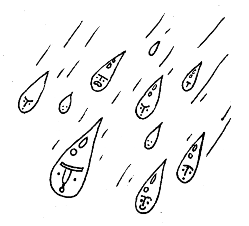
\includegraphics[scale=0.5]{16}}
\end{figure}
\end{SBSection*}
\end{song}

%\twocolumn
\begin{song}{Двадцать дней}{}{Сказка}{Сказка}{}{}


Двадцать дн\Ch{Dm}{ей} – это смена без дня.\par
“Маловато”,– вам скажут друзь\Ch{Gm}{я,}\par
А вожатый отв\Ch{C}{ет}ит люб\Ch{F}{ой}:\par
Это ср\Ch{Gm}{ок} очень д\Ch{A}{аж}е больш\Ch{Dm}{ой!}\\
 

Припев:\par
\ttМожно з\Ch{Gm C}{а-а-а-а} него усп\Ch{Dm}{ет}ь,\par
\ttНаприм\Ch{Gm}{ер,} полмилли\Ch{A}{он}а песен сп\Ch{Dm}{еть,}\par
\ttНо не к\Ch{Gm}{ажд}ый ведь поймет,\par
\ttКак так быстро раскрыв\Ch{A}{ат}ься может р\Ch{Dm}{от!}\\


Для полярника это не срок:\par
Не успеет просохнуть носок.\par
А вожатый успеет подряд \par
Вымыть, высушить сотню ребят!\\

Припев:\par
\ttВедь за смену, как за год \par
\ttСтолько разных мелочей произойдет,\par
\ttНо пока что нам везет,\par
\ttНас начальство для чего-то бережёт.\\


\newpage
Хоть и длинными кажутся дни,\par
Но как миг пролетели они.\par
Будешь долго потом вспоминать,\par
Как в отбой ты любил слово «СПАААТЬ!!!»\\

Припев:\par
\tt          	— Говорят за двадцать дней \par
\tt          	Все узнаешь о напарнице своей…\par
\tt          	— Только это ерунда,\par
\tt          	Обо всем ты не узнаешь никогда!\\

Смена вряд ли даст ответ:\par
Ты нашел свое призванье или нет.\par
Так что надо продолжать,\par
Двадцать раз по двадцать суток отсчитать!\\

\begin{SBSection*}
\begin{figure}[b!]
\center{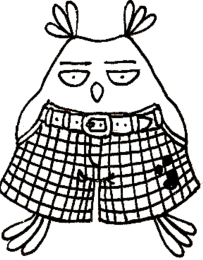
\includegraphics[scale=0.5]{17}}
\end{figure}
\end{SBSection*}

\end{song}

%\twocolumn
\begin{song}{Непогода}{}{Павел Смеян}{Павел Смеян}{}{}

\Ch{D}{Из}менения в природе \Ch{G}{пр}оисходят г\Ch{A}{од} от года,\par
\Ch{D}{Не}погода нынче в моде,\Ch{G}{} н\Ch{F#7}{епог}ода, непогода,\par
\Ch{}Hm{Слов}но из вод\Ch{F#7}{опро}вода \Ch{D7}{ль}ёт на нас с неб\Ch{G}{ес} во\Ch{Hm}{да…}\par
Полг\Ch{G}{од}а плох\Ch{A}{ая} пог\Ch{D}{од}а, \Ch{Hm}{пол}го\Ch{G}{да} — совс\Ch{A}{ем} нику\Ch{D}{да}.\par
Полг\Ch{G}{од}а плох\Ch{A}{ая} пог\Ch{D}{од}а, \Ch{Hm}{пол}го\Ch{G}{да} — сов\Ch{F#7}{сем} нику\Ch{Hm}{да.}\\


\SBChorusTagg:\par
\ttНикуда, нику\Ch{Em}{да н}ельз\Ch{A}{я} укр\Ch{D}{ы}ться н\Ch{Hm}{ам,}\par
\ttНо откладывать ж\Ch{Em}{изнь} ни\Ch{A}{как} нель\Ch{D}{зя}, \Ch{Hm}{}\par
\ttНикуда, нику\Ch{Em}{да, н}о зн\Ch{A}{ай}, что гд\Ch{D}{е}-то т\Ch{Hm}{ам}\par
\ttКто-то ищет теб\Ch{G}{я} сре\Ch{F#7}{ди д}ожд\Ch{Hm}{я.} \Ch{A}{}\\


Грома грозные раскаты от заката до восхода,\par
За грехи людские плата — непогода, непогода,\par
Не ангина, не простуда, посерьёзнее беда.\par
Полгода плохая погода, полгода — совсем никуда\par,
Полгода плохая погода, полгода — совсем никуда.\\\


\SBChorusTagg:\par
\ttНикуда, нику\Ch{Em}{да н}ельз\Ch{A}{я} укр\Ch{D}{ы}ться н\Ch{Hm}{ам,}\par
\ttНо откладывать ж\Ch{Em}{изнь} ни\Ch{A}{как} нель\Ch{D}{зя}, \Ch{Hm}{}\par
\ttНикуда, нику\Ch{Em}{да, н}о зн\Ch{A}{ай}, что гд\Ch{D}{е}-то т\Ch{Hm}{ам}\par
\ttКто-то ищет теб\Ch{G}{я} сре\Ch{F#7}{ди д}ожд\Ch{Hm}{я.} \Ch{A}{}\\


\end{song}

%\twocolumn
\begin{song}{Птенцы}{}{Сказка}{Сказка}{}{}

\Ch{Am}{}  \Ch{Am}{}

Как птенцы из гнез\Ch{Dm}{да} мы \Ch{E}{вы}па\Ch{Am}{ли.}\par
Ты не бойся при\Ch{Dm}{хо}да \Ch{G}{ве}че\Ch{C}{ра.}\par
Под та\Ch{A7}{ки}ми боль\Ch{F}{ши}ми \Ch{A7}{ли}па\Ch{Dm}{ми}\par
Нам с то\Ch{F}{бой} опа\Ch{Dm}{сать}ся \Ch{F}{не}\Ch{E}{че}\Ch{Am}{го.}\\
 
Под такими густыми звёздами -\par
Разве их не для нас рассыпали,\par
Мы не против гнездовья - просто мы\par
Из него ненароком выпали.\\

Это только вначале кажется,\par
Что без дома прожить нельзя никак,\par
Что важней пропитанья кашица,\par
Чем огромные звёзды на небе.\\

Ты не бойся ни тьмы, ни холода.\par
Будет день и найдётся пища нам,\par
Мы ещё пролетим над городом\par
На крыле до небес возвышенном.\\

Пролетим ещё - эка невидаль\par
Над Нью-Йорком, Парижем, Триполи\par
И над липой, откуда некогда,\par
Как птенцы из гнезда мы выпали.\\

Как птенцы из гнезда мы выпали.\par
Ты не бойся прихода вечера.\par
Под такими большими липами\par
Нам с тобой опасаться нечего.\\

\end{song}

%\twocolumn
\begin{song}{Продавец зонтиков}{}{Веня Дркин}{Веня Дркин}{}{}

\Ch{Am}{Город} этот выдумал о\Ch{Dm}{дин} художник,\par
\Ch{G}{Лю}ди в нем не знали, что та\Ch{C}{ко}е дождик.\par
\Ch{A7}{Про}сто не слыхали, что та\Ch{Dm}{ко}е зонтик –\par
\Ch{E7}{Вот} такие люди жили в \Ch{Am}{го}роде том.\par
И один чудак, в старый плащ одетый,\par
Продавал там зонтики зимой и летом,\par
Продавал там зонтики зимой и летом\par
И такую песенку он напевал:\\

\SBChorusTagg:\par
\tt“Господа, купите зонтик.\par
\ttБелый зонтик, красный зонтик,\par
\ttЖелтый зонтик, синий зонтик –\par
\ttМожет пригодится вам.”\\

Были домики у них из пластилина,\par
Из пустых коробочек автомашины,\par
И, не опасаясь никакой ангины,\par
Маленькие люди жили в городе том.\par
Маленькие были у людей заботы:\par
Шли они в кино или в театр с работы.\par
Вечером в подъезде целовался кто-то.\par
Все шутили и смеялись над стариком.\\


\SBChorusTagg.\\

\newpage

Маленькое небо как-то вдруг намокло,\par
В крошечных домишках задрожали стекла,\par
И огромный дождь пошел гулять по крышам,\par
Сразу все схватили насморк в городе том.\par
Вспомнили тут люди о торговце старом,\par
Кинулись искать его по всем базарам,\par
Но исчез торговец со своим товаром.\par
Только песенка осталась в память о нем:\\

\SBChorusTagg.\par

\begin{SBSection*}
\begin{figure}[b!]
\center{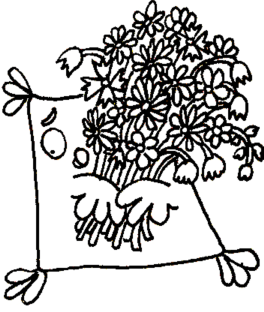
\includegraphics[scale=0.5]{15}}
\end{figure}
\end{SBSection*}

\end{song}

%\twocolumn
\begin{song}{Белая гвардия}{}{Белая гвардия}{Белая гвардия}{}{}

Проигрыш: (2 раза)\par 
\Ch{Am}{} \Ch{D}{} \Ch{G}{} \Ch{C}{} \Ch{Am}{} \Ch{H7}{} \Ch{Em}\\

\Ch{Em}{Белая} гвардия, белый снег,\par
\Ch{Am7}{Белая} музыка революций.\par
\Ch{D7}{Белая} женщина, нервный смех,\par
\Ch{G}{Белого} платья слегка коснуться.\par
 
Белой рукой распахнуть окно,\par
Белого света в нем не видя.\par
Белое выпить до дна вино,\par
В красную улицу в белом выйти.\\

Припев:\par
\ttКог\Ch{Em}{да} ты вернешься,\par
\ttВсе будет и\Ch{Am}{на}че, и нам бы узнать друг друга,\par
\ttКог\Ch{D7}{да} ты вернешься,\par
\ttА я не же\Ch{G}{на} и даже \Ch{H7}{не} подруга.\par
\ttКог\Ch{C}{да} ты вернешься,\par
\ttКо мне, так без\Ch{Am}{ум}но тебя любившей в прошлом,\par
\tt\Ch{D7}{Ко}гда ты вернешься -\par
\ttУвидишь, что ж\Ch{G}{ре}бий давно и не \Ch{E7}{нами} брошен.\\

Проигрыш.\\
 
\newpage
Сизые сумерки прошлых лет\par
Робко крадутся по переулкам.\par
В этом окне еле брезжит свет,\par
Ноты истрепаны, звуки гулки.\par
Тонкие пальцы срывают аккорд...\par
Нам не простят безрассудного дара.\par
Бьются в решетку стальных ворот\par
Пять океанов земного шара.\\

Припев. \par
Проигрыш.\\
 
Красный трамвай простучал в ночи,\par
Красный закат догорел в бокале,\par
Красные-красные кумачи\par
С красных деревьев на землю упали.\par
Я не ждала тебя в октябре,\par
Виделись сны, я листала сонник:\par
Красные лошади на заре\par
Били копытами о подоконник.\\

Припев:\par
\ttКогда ты вернешься,\par
\ttВсе будет иначе, и нам бы узнать друг друга,\par
\ttКогда ты вернешься,\par
\ttА я не жена и даже не подруга.\par
\ttКогда ты вернешься,\par
\ttВернешься в наш город обетованный,\par
\ttКогда ты вернешься -\par
\ttТакой невозможный и такой желанный?\\

Проигрыш.\par

\end{song}

%\twocolumn
\begin{song}{Перевал}{}{Песни у костра}{Песни у костра}{}{}


\Ch{Am}{Про}сто нечего нам \Ch{Dm}{боль}ше терять\par
\Ch{E}{Всё} нам вспомнится на \Ch{Am}{Страшном} суде.\par
Эта ночь легла, как \Ch{Dm}{тот} перевал,\par
\Ch{G}{За} которым испол\Ch{C}{нень}е надежд.\par
\Ch{A7}{Про}сто прожитое—про\Ch{Dm}{жи}то зря, \Ch{G}{}\par
Но не в этом, пони\Ch{C}{мае}шь ли, соль… \Ch{Am}{}\par
Слышишь, падают дож\Ch{Dm}{ди} октября.\par
\Ch{E}{Ви}дишь, старый дом сто\Ch{Am}{ит} средь лесов.\\

Мы затопим в доме печь, в доме печь,\par
Мы гитару позовем со стены.\par
Просто нечего нам больше беречь,\par
Ведь за нами все мосты сожжены.\par
Все мосты, все перекрёстки дорог,\par
Все прошёптанные тайны в ночи.\par
Каждый сделал все, что смог, все, что смог,\par
Мы об этом помолчим, помолчим.\\


И луна взойдет заплывшей свечой,\par
Ставни скрипнут  на ветру, на ветру.\par
Ах, как я тебя люблю горячо,\par
Это годы не сотрут, не сотрут.\par
Мы оставшихся друзей соберем,\par
Мы набьем картошкой старый рюкзак,\par
Люди спросят: "Что за шум, что за гам?"\par
Мы ответим: "Просто так,  просто так”...\\

\newpage

    Просто так идут дожди в октябре,\par
    И потеряны от счастья ключи.\par
    Это всё, конечно, мне, конечно, мне,\par
    Но об этом помолчим, помолчим.\par
    Просто прожитое—прожито зря,\par
    Но не в этом, понимаешь ли, соль…\par
    Слышишь, падают дожди октября.\par
    Видишь, старый дом стоит средь лесов.\par


\begin{SBSection*}
\begin{figure}[b!]
\center{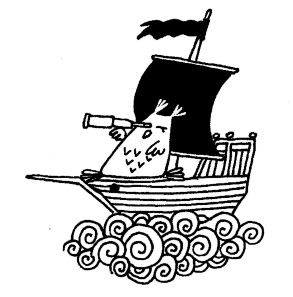
\includegraphics[scale=0.5]{22}}
\end{figure}
\end{SBSection*}

\end{song}

%\twocolumn
\begin{song}{Ленинградская (Все расстояния)}{}{Песни у костра}{Песни у костра}{}{}

\Ch{Am}{Все} расстоянья когда-нибудь в круг замы\Ch{E}{ка}ются,\par
\Ch{E}{Все} из разлук обязательно \Ch{E7}{встре}чей кон\Ch{Am}{ча}ются;\par
Должны про\Ch{Dm}{плыть} вокруг Зем\Ch{G}{ли,}\par
Вернуться в \Ch{C}{га}вань кораб\Ch{F}{ли,}\par   
Все поез\Ch{Dm}{да} в свои вер\Ch{E}{нуть}ся горо\Ch{Am}{да.}\\
 
Шумный вокзал то встречает друзей , то прощается,\par
Мы расстаемся, но снова назад возвращаемся -\par
Чтоб снова встать в огромный круг,\par
И снова знать, что рядом друг ,\par
И песни петь, чтоб больше не было разлук.\\
 
Все расстоянья когда-нибудь в круг замыкаются,\par
Все из разлук обязательно встречей кончаются;\par
И через год, и через пять,\par
Мы с вами встретимся опять,\par
Ничто не сможет нашей дружбе помешать.\par

\end{song}

%\twocolumn
\begin{song}{Десять капель}{}{Танцы Минус}{Танцы Минус}{}{}

Проигрыш: (2 раза)\par 
\Ch{C}{} \Ch{E}{} \Ch{Am}{} \Ch{F}{} \Ch{C}{} \Ch{E}{} \Ch{Am}{} \Ch{F}{}

\Ch{C}{Де}сять капель дож\Ch{E}{дя} у тебя на пле\Ch{Am}{че}\par
Ты забыла свой \Ch{F}{зонт,} ты спешила ко \Ch{C}{мне.}\par
Десять капель дож\Ch{E}{дя} на плече у те\Ch{Am}{бя,}\par
Десять капель люб\Ch{F}{ви,} десять капель ог\Ch{C}{ня}\\

Припев:\\(Три первых слова в припеве дублируются вторым голосом)\par
\tt\Ch{C}{Т}воя\Ch{E}{} ладо\Ch{Am}{нь} горит\Ch{F}{} в моих руках\par
\tt\Ch{C}{Л}юбви\Ch{E}{ }пож\Ch{Am}{ар} горит в тво\Ch{F}{их} глазах\\

Проигрыш.\\

Время делает шаг, время делает круг\par
Мы забудем друзей, мы забудем подруг\par
Просто выпьем вина из любви и огня\par
Десять капель меня, десять капель тебя\\

Припев.\\

Голос твой в тишине околдует меня\par
Ярким жарким огнем стану я до утра\par
Ты прикажешь гори, и я вспыхну любя\par
В этом пламени ты, в этом пламени я.\par

\end{song}

%\twocolumn
\begin{song}{Макет}{}{Песни у костра}{Сказка}{}{}
sadfsfthanks,\par
\begin{SBOpGroup}
asdas\
\end{SBOpGroup}
\begin{SBSection*}fdf\end{SBSection*}
\begin{SBVerse*}\end{SBVerse*}
\begin{SBChorus*}\end{SBChorus*}

\begin{SBOccurs}{23}
dsf
\end{SBOccurs}

\begin{SBSection*}
\begin{figure}[b!]
\center{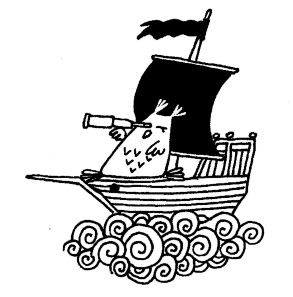
\includegraphics[scale=0.5]{22}}
\end{figure}
\end{SBSection*}
\end{song}

\mainmatter

\renewcommand{\footrulewidth}{0.0pt}
\renewcommand{\item}{\par\hangindent=40pt}
\renewcommand{\subitem}{\par\hangindent=40pt \hspace*{20pt}}
\renewcommand{\subsubitem}{\par\hangindent=40pt \hspace*{30pt}}

\newpage
\raggedright%\documentclass[a5paper,11pt]{book}
%\usepackage{fancyhdr}
%\usepackage[chordbk]{songbook}
%
%\usepackage[T2A]{fontenc}
%\usepackage[utf8]{inputenc}
%\usepackage[russian]{babel}
%
%\title{A Church Songbook}
%\author{}
%\date{Revised:  \RevDate}
%
%\newcommand{\RelDate}{13 November'19}
%\newcommand{\RevDate}{\today}

\documentclass[11pt,a5paper]{book}
\usepackage[a5paper]{geometry}
\usepackage[chordbk]{songbook}
\usepackage[T2A]{fontenc}
\usepackage[utf8]{inputenc}
\usepackage[russian]{babel}
\usepackage{cmap} % для работы поиска кириллицы в pdf

%\usepackage{amsmath,amsthm,amssymb}
%\usepackage{mathtext}


\usepackage[pdftex]{graphicx}
\usepackage{lscape}
%\usepackage{vmargin}
\usepackage{textcomp}
\usepackage{setspace}
%\usepackage{marvosym}
\usepackage{gensymb} %%%for \micro tag
\usepackage{upgreek} %%% \upmu
\usepackage{tipa}
\usepackage{phonetic}
%\usepackage[greek,english]{babel}
\usepackage{threeparttable}
\usepackage{multirow}
\usepackage{harvard}
\usepackage{longtable}
\renewcommand{\sectionmark}[1]{\markright{#1}}
\renewcommand{\chaptermark}[1]{\markboth{#1}{}}
\addto\captionsenglish{\renewcommand{\bibname}{References}}
\usepackage{latexsym,fancyhdr}

\newcommand{\RelDate}{26 Апреля'1984}
\newcommand{\RevDate}{\today}

%%%
% C.C.L.I. license number definition; for copyright licensing info.
% One of these macros will be manually inserted into the {CpyRt}
% parameter of the {song} environment.
%
%       \CCLInumber - The actual copyright license number.  Don't
%               insert this command in the {CpyRt} parameter, use one
%               of the others.
%       \CCLIed - Indicates a song falls under our CCLI license.
%       \NotCCLIed - Indicates a song doesn't fall under our CCLI
%               license.  Public Domain songs fall into this category.
%       \PGranted - We have received specific permission from the
%               copyright holder to use this song.
%       \PPending - We are in the process of obtaining permission to
%               use this song.
%%%
\newcommand{\CCLInumber}{Your CCLI Number}
\newcommand{\CCLIed}{{\CpyRtInfoFont (CCLI \CCLInumber)}}
\newcommand{\NotCCLIed}{\relax}
\newcommand{\PGranted}{\relax}
\newcommand{\PPending}{{\CpyRtInfoFont (Permission Pending)}}

%%%
% Title page information.
%%%
\title{ Сказочный песенник}
\author{}
\date{Созданно:  \RevDate}


%%%
% Define fonts to use in the headers and footers of the songbook.
%%%
\newcommand{\LHeadFont}{\normalsize}            % = cmr12  at 12pt
\newcommand{\CHeadFont}{\normalsize\rm}         % = cmr12  at 12pt
\newcommand{\RHeadFont}{\normalsize}            % = cmr12  at 12pt
\newcommand{\LFootFont}{\scriptsize}            % = cmr8   at  8pt
\newcommand{\CFootFont}{\tiny\myTinySF}         % = cmss8  at  8pt
\newcommand{\RFootFont}{\scriptsize}            % = cmr8   at  8pt

%%%
% Turn on and define fancy page heading/footing definition.
%%%
\pagestyle{fancy}

\ifChordBk
  % It's a words & chords songbook...
%  \addtolength{\headwidth}{\marginparsep}
%  \addtolength{\headwidth}{\marginparwidth}
  \renewcommand{\headrulewidth}{0.0pt}
  \renewcommand{\footrulewidth}{0.0pt}
%  \fancyhead[LE,RO]{\LHeadFont\emph{\leftmark\/}}
%  \fancyhead[CE,CO]{\CHeadFont\thepage}
  \fancyhead[RE,LO]{~}
\else\ifOverhead
  % It's an overhead...
  \renewcommand{\footrulewidth}{0pt}
  \renewcommand{\headrulewidth}{0pt}
  \fancyhead[LE,RO]{}
  \fancyhead[CE,CO]{}
  \fancyhead[RE,LO]{}
\else\ifWordBk
  % It's a words only songbook...
  \addtolength{\headwidth}{\marginparsep}
  \addtolength{\headwidth}{\marginparwidth}
  \renewcommand{\headrulewidth}{0.0pt}
  \renewcommand{\footrulewidth}{0.0pt}
  \fancyhead[LE,RO]{\LHeadFont A Church Songbook}
  \fancyhead[CE,CO]{\CHeadFont\thepage}
  \fancyhead[RE,LO]{\RHeadFont\RelDate}
\fi\fi\fi

%\fancyfoot[LE,RO]{\LFootFont Property of The Church}
%\ifSongEject
%  \fancyfoot[CE,CO]{\CFootFont \RevDate}
%\else
%  \fancyfoot[CE,CO]{\CFootFont}
%\fi
%\fancyfoot[RE,LO]{\RFootFont Material used by permission.}

%%%
% Turn on/off index-file generation.  Uncomment the \makeindex line to
% turn index generation on;  comment it out to turn index generation
% off.
%%%
\makeTitleIndex         %% Title and First Line Index.
\makeTitleContents      %% Table of Contents.
\makeKeyIndex           %% Index of song by key.
\graphicspath{{img/}} % папка с картинками
\DeclareGraphicsExtensions{.pdf,.png,.jpg} % форматы, которые будем считать картинками

%\newenvironment{song}[7][Y]{
%% Comment markers to negate
%\if#1Y\ExcludeSongfalse\else\ExcludeSongtrue\fi% the newline.
%\ifPrintAllSongs\ExcludeSongfalse\fi
%\SongMarkboth{\relax}{\relax}
%\SBinSongEnvtrue
%\renewcommand{\SBinSongEnv}{\True}
%\ifWordsOnly
%	\setlength{\parindent}{0pt}
%\fi

%%%
% Redefine fonts from SongBook style that I don't like.
%%%
\font\myTinySF=cmss8 at 8pt
\renewcommand{\CpyRtInfoFont}{\tiny\myTinySF}


%
%\font\myTinySF=cmss8    at  8pt
%\font\myHugeSF=cmssbx10 at 25pt
%\renewcommand{\CpyRtInfoFont}{\tiny\myTinySF}
%\newcommand{\myTitleFont}{\Huge\myHugeSF}
%\newcommand{\mySubTitleFont}{\large\sf}

%%% Работа с русским языком
%\usepackage[no-math]{fontspec}      %% подготавливает загрузку шрифтов Open Type, True Type и др.
%\defaultfontfeatures{Ligatures={TeX},Renderer=Basic}  %% свойства шрифтов по умолчанию
%\setmainfont[Ligatures={TeX,Historic}]{Times New Roman} %% задаёт основной шрифт документа
%\setsansfont{Helvetica Neue}                    %% задаёт шрифт без засечек

%\newfontfamily{\allods}{AllodsWest}

\newcommand{\SBPubDomm}{~}
\renewcommand{\CpyRt}[3][Y]{%
\if#1Y\begin{center}\fi
\if\blank{#2}%
\if\blank{#3}%
{\CpyRtFont\copyright \SBUnknownTag{} \CpyRtInfoFont}%
\else
{\CpyRtFont\copyright \SBUnknownTag{} \CpyRtInfoFont #3}%
\fi%
\else%
\ifthenelse{\equal{#2}{\SBPubDomm}}
{%then
{\CpyRtFont #2 \CpyRtInfoFont #3}%
}{%else
{\CpyRtFont #2 \CpyRtInfoFont #3}%
}%fi
\fi%
\if#1Y\end{center}\fi
}


\newcommand{\SBUnknownTagg}{~}
\renewcommand{\WAndM}[2][Y]{~}
\renewcommand{\WAndM}[2][Y]{%
\if#1Y\begin{center}\fi
\if\blank{#2}%
{\SBUnknownTagg}%
\else
{~}%
\fi
\if#1Y\end{center}\fi
}

\renewcommand{\STitle}[3][Y]{%
\setcounter{SBVerseCnt}{0}%
\setcounter{SBSectionCnt}{0}%
\ifExcludeSong\relax%
	\else\keyIndex{{\protect\sbChord#3\protect\relax} -- #2}{\theSBSongCnt}\fi%
	\vspace{\SpaceAboveSTitle}%
\if#1Y\begin{center}\fi
	{}{\STitleFont\LARGE #2}%
	\ifWordsOnly\relax\else\fi%
	\if#1Y\end{center}\fi
\STitleMarkboth{#2}{\relax}%
}


%\renewenvironment{SBOpGroup}{%
%	\sbSetsbBaselineSkipAmt%
%	\bgroup%
%	\begin{list}{\hbox{}}
%	  {\setlength {\leftmargin}
%		{\HangAmt}
%		\setlength{\itemindent}
%			{-\HangAmt}
%		\setlength{\listparindent}{-\HangAmt}
%		\setlength{\topsep}{0pt}
%		\setlength{\parsep}{0pt}
%		\setlength{\labelwidth}{0pt}
%		\setlength{\labelsep}{0pt}
%		\setlength{\baselineskip} {\sbBaselineSkipAmt}
%	}%\item}
%{\end{list}%
\newcommand{\SBChorusTagg}{Припев}
\renewenvironment{SBChorus}{%
\sbSetsbBaselineSkipAmt%
\bgroup%
\SBChorusMarkright{\SBChorusTag}
\begin{list}{{\SBChorusTagFont\SBChorusTagg}}
{\setlength {\leftmargin}
{\LeftMarginSBChorus + \HangAmt}
\setlength{\itemindent}
{-\HangAmt}
\setlength{\listparindent}{-\HangAmt}
\setlength{\parsep}
{0pt}
\setlength{\baselineskip} {\sbBaselineSkipAmt}
}%
\item}
{\end{list}%
\egroup%
\SpaceAfterChorus%
}

\renewcommand{\tt}{\indent \indent}
%\renewcommand{\nt}{\noindent}


\usepackage{amsmath}

\makeArtistIndex
\makeTitleIndex         %% Title and First Line Index.
\makeTitleContents      %% Table of Contents.
\makeKeyIndex           %% Index of song by key.
%\usepackage{printallsongs}

\begin{document} 
\maketitle

\mainmatter


\begin{song}{Вожатский гимн}{}{Сказка}{Сказка}{}{}

По \Ch{Am}{ла}герю подъём, нас горн зовёт!\par
Забудь о том, что ночь была бес\Ch{C}{сон}ною\par
Смо\Ch{Dm}{чи} водою \Ch{G}{ве}ки воспа\Ch{C}{лён}\Ch{F}{ные}\par    
По\Ch{Dm}{вя}зывай свой \Ch{E}{галс}тук — и впе\Ch{Am (A7)}{рёд!}\par
Смо\Ch{Dm}{чи} водою \Ch{G}{ве}ки воспа\Ch{C}{лён}\Ch{F}{ные}\par    
По\Ch{Dm}{вя}зывай свой \Ch{E}{галс}тук — и впе\Ch{Am (A7)}{рёд!}\par

%	\begin{SBChorus*}
\ttНе\Ch{E}{про}сто воспитывать \Ch{Am}{но}вых людей,\par
\ttНу \Ch{E}{что} ж, это наша с то\Ch{Am}{бою} свя\Ch{A7}{ты}ня.\par
\ttМой \Ch{Dm}{друг}, нам до\Ch{G}{ве}рили \Ch{C}{ду}ши де\Ch{F}{тей},\par
\ttИх \Ch{Dm}{ра}достный \Ch{Am}{смех} нам на\Ch{E}{гра}да от\Ch{Am}{ны}не.\par
\ttМой \Ch{Dm}{друг}, нам до\Ch{G}{ве}рили \Ch{C}{ду}ши де\Ch{F}{тей},\par
\ttИх \Ch{Dm}{ра}достный \Ch{Am}{смех} нам на\Ch{E}{гра}да от\Ch{Am}{ны}не.\\
%\end{SBChorus*}

Отбой, засыпает детвора.\par
Взгляни на их улыбки полусонные,\par
Пускай им снятся острова зелёные,\par
А нам опять работать до утра!\par
Пускай им снятся острова зелёные,\par
А нам опять работать до утра!\par

\tt И пусть от бессилья затихнешь не раз,\par
\ttИ голос усталый до хрипа натружен,\par
\ttПусть будут умней и счастливее нас\par
\ttТе дети, в которых вложили мы души!\par
\ttПусть будут умней и счастливее нас\par
\ttТе дети, в которых вложили мы души!

\end{song}

\begin{song}{Сказка в неглиже}{}{Сказка}{Сказка}{}{}

Есть у \Ch{C}{каж}дого добрая сказка в ду\Ch{F}{ше,}\par 
Надо \Ch{G}{толь}ко прочесть этой сказки стра\Ch{C}{ни}цы.\par
В тиши\Ch{C}{не}, разо\Ch{C7}{де}тая вся в негли\Ch{F}{же,}\par
Пусть на\Ch{G}{ве}ки она, пусть на\Ch{F}{ве}ки она сохра\Ch{C}{ни}тся. \Ch{C7}{ }\par 
В тиши\Ch{F}{не,} разо\Ch{G}{де}тая вся в негли\Ch{C}{же,} \Ch{Am}{}\par
Пусть на\Ch{F}{ве}ки она, пусть на\Ch{G}{ве}ки она сохра\Ch{C}{ни}тся.\\


\ttЭту сказку пред другом раскрыть поспеши,\par
\ttА врагу не спеши эту сказку поведать.\par
\ttПусть растут и читают ее малыши.\par
\ttБудь добрей, и тебя минут всякие беды.\par
\ttПусть растут и читают ее малыши.\par
\ttБудь добрей, и тебя минут всякие беды.\\


\Ch{C7}{}Будет \Ch{F}{мно}го распутий, \Ch{G}{до}рог и тре\Ch{C}{вог.}\Ch{Am}{}\par
На вис\Ch{F}{ки} твои ляжет \Ch{G}{не}тающий \Ch{C}{ин}ей, \Ch{C7}{}\par
И пой\Ch{F}{мёшь,} научившись чи\Ch{G}{тать} между \Ch{C}{строк:} \Ch{Am}{}\par
Даже \Ch{F}{гнус}ный злодей \Ch{G}{в} этой сказке не\Ch{C}{ви}нен. \Ch{C7}{}\par
И пой\Ch{F}{мёшь,} научившись чи\Ch{G}{тать} между ст\Ch{C}{рок:} \Ch{A}{}\par
Даже \Ch{F}{гнус}ный злодей \Ch{G}{в} этой сказке не\Ch{C}{ви}нен.\\

\Ch{C}{} \Ch{G}{} \Ch{F}{} \Ch{G}{} \Ch{C}{} \Ch{C7}{}\par
\Ch{C}{} \Ch{G}{} \Ch{F}{} \Ch{G}{} \Ch{C}{}
\end{song}

%\twocolumn
\begin{song}{Вожатский марш}{}{Сказка}{Сказка}{}{}

Есть на\Ch{Am}{род} у нас весёлый,\par
Самой \Ch{C}{луч}шей в мире пробы,\par
Песни \Ch{G}{петь} всегда мас\Ch{C}{так.}\Ch{A7}{}\par
Он всег\Ch{Dm}{да} всего добьётся,\par
Он Вожа\Ch{Am}{ты}ми зовётся,\par
\Ch{E}{Так} и только \Ch{Am (A7)}{так!}\par
Он всег\Ch{Dm}{да} всего добьётся,\par
Он Во\Ch{Am}{жа}тыми зовётся,\par
\Ch{E}{Так} и только \Ch{Am (A7)}{так!}\\

Домосед привязан к дому\par
И по случаю такому,\par
Он из дома — ни на шаг!\par
А вожатый — он в дороге,\par
Он готов в огонь и в воду,\par
Так и только так!\par
А вожатый — он в дороге,\par
Он готов в огонь и в воду,\par
Так и только так!\\
\newpage
Жадный денежки считает,\par
Все считает и считает,\par
К пятаку кладет пятак.\par
А вожатый деньги тратит,\par
Не боясь, что их не хватит,\par
Так и только так!\par
А вожатый деньги тратит,\par
Не боясь, что их не хватит,\par
Так и только так!\\

Холостяк в любовь не верит,\par
Все не верит и не верит,\par
Потому что холостяк.\par
А вожатых не влюблённых\par
Не найдёшь определённо,\par
Так и только так!\par
А вожатых не влюблённых\par
Не найдёшь определённо,\par
Так и только так!\par

\begin{SBSection*}
\begin{figure}[b!]
\center{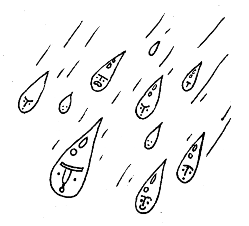
\includegraphics[scale=0.5]{16}}
\end{figure}
\end{SBSection*}
\end{song}

%\twocolumn
\begin{song}{Двадцать дней}{}{Сказка}{Сказка}{}{}


Двадцать дн\Ch{Dm}{ей} – это смена без дня.\par
“Маловато”,– вам скажут друзь\Ch{Gm}{я,}\par
А вожатый отв\Ch{C}{ет}ит люб\Ch{F}{ой}:\par
Это ср\Ch{Gm}{ок} очень д\Ch{A}{аж}е больш\Ch{Dm}{ой!}\\
 

Припев:\par
\ttМожно з\Ch{Gm C}{а-а-а-а} него усп\Ch{Dm}{ет}ь,\par
\ttНаприм\Ch{Gm}{ер,} полмилли\Ch{A}{он}а песен сп\Ch{Dm}{еть,}\par
\ttНо не к\Ch{Gm}{ажд}ый ведь поймет,\par
\ttКак так быстро раскрыв\Ch{A}{ат}ься может р\Ch{Dm}{от!}\\


Для полярника это не срок:\par
Не успеет просохнуть носок.\par
А вожатый успеет подряд \par
Вымыть, высушить сотню ребят!\\

Припев:\par
\ttВедь за смену, как за год \par
\ttСтолько разных мелочей произойдет,\par
\ttНо пока что нам везет,\par
\ttНас начальство для чего-то бережёт.\\


\newpage
Хоть и длинными кажутся дни,\par
Но как миг пролетели они.\par
Будешь долго потом вспоминать,\par
Как в отбой ты любил слово «СПАААТЬ!!!»\\

Припев:\par
\tt          	— Говорят за двадцать дней \par
\tt          	Все узнаешь о напарнице своей…\par
\tt          	— Только это ерунда,\par
\tt          	Обо всем ты не узнаешь никогда!\\

Смена вряд ли даст ответ:\par
Ты нашел свое призванье или нет.\par
Так что надо продолжать,\par
Двадцать раз по двадцать суток отсчитать!\\

\begin{SBSection*}
\begin{figure}[b!]
\center{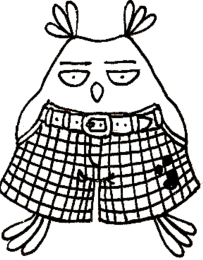
\includegraphics[scale=0.5]{17}}
\end{figure}
\end{SBSection*}

\end{song}

%\twocolumn
\begin{song}{Непогода}{}{Павел Смеян}{Павел Смеян}{}{}

\Ch{D}{Из}менения в природе \Ch{G}{пр}оисходят г\Ch{A}{од} от года,\par
\Ch{D}{Не}погода нынче в моде,\Ch{G}{} н\Ch{F#7}{епог}ода, непогода,\par
\Ch{}Hm{Слов}но из вод\Ch{F#7}{опро}вода \Ch{D7}{ль}ёт на нас с неб\Ch{G}{ес} во\Ch{Hm}{да…}\par
Полг\Ch{G}{од}а плох\Ch{A}{ая} пог\Ch{D}{од}а, \Ch{Hm}{пол}го\Ch{G}{да} — совс\Ch{A}{ем} нику\Ch{D}{да}.\par
Полг\Ch{G}{од}а плох\Ch{A}{ая} пог\Ch{D}{од}а, \Ch{Hm}{пол}го\Ch{G}{да} — сов\Ch{F#7}{сем} нику\Ch{Hm}{да.}\\


\SBChorusTagg:\par
\ttНикуда, нику\Ch{Em}{да н}ельз\Ch{A}{я} укр\Ch{D}{ы}ться н\Ch{Hm}{ам,}\par
\ttНо откладывать ж\Ch{Em}{изнь} ни\Ch{A}{как} нель\Ch{D}{зя}, \Ch{Hm}{}\par
\ttНикуда, нику\Ch{Em}{да, н}о зн\Ch{A}{ай}, что гд\Ch{D}{е}-то т\Ch{Hm}{ам}\par
\ttКто-то ищет теб\Ch{G}{я} сре\Ch{F#7}{ди д}ожд\Ch{Hm}{я.} \Ch{A}{}\\


Грома грозные раскаты от заката до восхода,\par
За грехи людские плата — непогода, непогода,\par
Не ангина, не простуда, посерьёзнее беда.\par
Полгода плохая погода, полгода — совсем никуда\par,
Полгода плохая погода, полгода — совсем никуда.\\\


\SBChorusTagg:\par
\ttНикуда, нику\Ch{Em}{да н}ельз\Ch{A}{я} укр\Ch{D}{ы}ться н\Ch{Hm}{ам,}\par
\ttНо откладывать ж\Ch{Em}{изнь} ни\Ch{A}{как} нель\Ch{D}{зя}, \Ch{Hm}{}\par
\ttНикуда, нику\Ch{Em}{да, н}о зн\Ch{A}{ай}, что гд\Ch{D}{е}-то т\Ch{Hm}{ам}\par
\ttКто-то ищет теб\Ch{G}{я} сре\Ch{F#7}{ди д}ожд\Ch{Hm}{я.} \Ch{A}{}\\


\end{song}

%\twocolumn
\begin{song}{Птенцы}{}{Сказка}{Сказка}{}{}

\Ch{Am}{}  \Ch{Am}{}

Как птенцы из гнез\Ch{Dm}{да} мы \Ch{E}{вы}па\Ch{Am}{ли.}\par
Ты не бойся при\Ch{Dm}{хо}да \Ch{G}{ве}че\Ch{C}{ра.}\par
Под та\Ch{A7}{ки}ми боль\Ch{F}{ши}ми \Ch{A7}{ли}па\Ch{Dm}{ми}\par
Нам с то\Ch{F}{бой} опа\Ch{Dm}{сать}ся \Ch{F}{не}\Ch{E}{че}\Ch{Am}{го.}\\
 
Под такими густыми звёздами -\par
Разве их не для нас рассыпали,\par
Мы не против гнездовья - просто мы\par
Из него ненароком выпали.\\

Это только вначале кажется,\par
Что без дома прожить нельзя никак,\par
Что важней пропитанья кашица,\par
Чем огромные звёзды на небе.\\

Ты не бойся ни тьмы, ни холода.\par
Будет день и найдётся пища нам,\par
Мы ещё пролетим над городом\par
На крыле до небес возвышенном.\\

Пролетим ещё - эка невидаль\par
Над Нью-Йорком, Парижем, Триполи\par
И над липой, откуда некогда,\par
Как птенцы из гнезда мы выпали.\\

Как птенцы из гнезда мы выпали.\par
Ты не бойся прихода вечера.\par
Под такими большими липами\par
Нам с тобой опасаться нечего.\\

\end{song}

%\twocolumn
\begin{song}{Продавец зонтиков}{}{Веня Дркин}{Веня Дркин}{}{}

\Ch{Am}{Город} этот выдумал о\Ch{Dm}{дин} художник,\par
\Ch{G}{Лю}ди в нем не знали, что та\Ch{C}{ко}е дождик.\par
\Ch{A7}{Про}сто не слыхали, что та\Ch{Dm}{ко}е зонтик –\par
\Ch{E7}{Вот} такие люди жили в \Ch{Am}{го}роде том.\par
И один чудак, в старый плащ одетый,\par
Продавал там зонтики зимой и летом,\par
Продавал там зонтики зимой и летом\par
И такую песенку он напевал:\\

\SBChorusTagg:\par
\tt“Господа, купите зонтик.\par
\ttБелый зонтик, красный зонтик,\par
\ttЖелтый зонтик, синий зонтик –\par
\ttМожет пригодится вам.”\\

Были домики у них из пластилина,\par
Из пустых коробочек автомашины,\par
И, не опасаясь никакой ангины,\par
Маленькие люди жили в городе том.\par
Маленькие были у людей заботы:\par
Шли они в кино или в театр с работы.\par
Вечером в подъезде целовался кто-то.\par
Все шутили и смеялись над стариком.\\


\SBChorusTagg.\\

\newpage

Маленькое небо как-то вдруг намокло,\par
В крошечных домишках задрожали стекла,\par
И огромный дождь пошел гулять по крышам,\par
Сразу все схватили насморк в городе том.\par
Вспомнили тут люди о торговце старом,\par
Кинулись искать его по всем базарам,\par
Но исчез торговец со своим товаром.\par
Только песенка осталась в память о нем:\\

\SBChorusTagg.\par

\begin{SBSection*}
\begin{figure}[b!]
\center{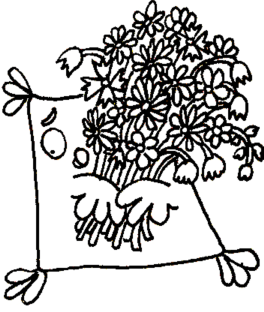
\includegraphics[scale=0.5]{15}}
\end{figure}
\end{SBSection*}

\end{song}

%\twocolumn
\begin{song}{Белая гвардия}{}{Белая гвардия}{Белая гвардия}{}{}

Проигрыш: (2 раза)\par 
\Ch{Am}{} \Ch{D}{} \Ch{G}{} \Ch{C}{} \Ch{Am}{} \Ch{H7}{} \Ch{Em}\\

\Ch{Em}{Белая} гвардия, белый снег,\par
\Ch{Am7}{Белая} музыка революций.\par
\Ch{D7}{Белая} женщина, нервный смех,\par
\Ch{G}{Белого} платья слегка коснуться.\par
 
Белой рукой распахнуть окно,\par
Белого света в нем не видя.\par
Белое выпить до дна вино,\par
В красную улицу в белом выйти.\\

Припев:\par
\ttКог\Ch{Em}{да} ты вернешься,\par
\ttВсе будет и\Ch{Am}{на}че, и нам бы узнать друг друга,\par
\ttКог\Ch{D7}{да} ты вернешься,\par
\ttА я не же\Ch{G}{на} и даже \Ch{H7}{не} подруга.\par
\ttКог\Ch{C}{да} ты вернешься,\par
\ttКо мне, так без\Ch{Am}{ум}но тебя любившей в прошлом,\par
\tt\Ch{D7}{Ко}гда ты вернешься -\par
\ttУвидишь, что ж\Ch{G}{ре}бий давно и не \Ch{E7}{нами} брошен.\\

Проигрыш.\\
 
\newpage
Сизые сумерки прошлых лет\par
Робко крадутся по переулкам.\par
В этом окне еле брезжит свет,\par
Ноты истрепаны, звуки гулки.\par
Тонкие пальцы срывают аккорд...\par
Нам не простят безрассудного дара.\par
Бьются в решетку стальных ворот\par
Пять океанов земного шара.\\

Припев. \par
Проигрыш.\\
 
Красный трамвай простучал в ночи,\par
Красный закат догорел в бокале,\par
Красные-красные кумачи\par
С красных деревьев на землю упали.\par
Я не ждала тебя в октябре,\par
Виделись сны, я листала сонник:\par
Красные лошади на заре\par
Били копытами о подоконник.\\

Припев:\par
\ttКогда ты вернешься,\par
\ttВсе будет иначе, и нам бы узнать друг друга,\par
\ttКогда ты вернешься,\par
\ttА я не жена и даже не подруга.\par
\ttКогда ты вернешься,\par
\ttВернешься в наш город обетованный,\par
\ttКогда ты вернешься -\par
\ttТакой невозможный и такой желанный?\\

Проигрыш.\par

\end{song}

%\twocolumn
\begin{song}{Перевал}{}{Песни у костра}{Песни у костра}{}{}


\Ch{Am}{Про}сто нечего нам \Ch{Dm}{боль}ше терять\par
\Ch{E}{Всё} нам вспомнится на \Ch{Am}{Страшном} суде.\par
Эта ночь легла, как \Ch{Dm}{тот} перевал,\par
\Ch{G}{За} которым испол\Ch{C}{нень}е надежд.\par
\Ch{A7}{Про}сто прожитое—про\Ch{Dm}{жи}то зря, \Ch{G}{}\par
Но не в этом, пони\Ch{C}{мае}шь ли, соль… \Ch{Am}{}\par
Слышишь, падают дож\Ch{Dm}{ди} октября.\par
\Ch{E}{Ви}дишь, старый дом сто\Ch{Am}{ит} средь лесов.\\

Мы затопим в доме печь, в доме печь,\par
Мы гитару позовем со стены.\par
Просто нечего нам больше беречь,\par
Ведь за нами все мосты сожжены.\par
Все мосты, все перекрёстки дорог,\par
Все прошёптанные тайны в ночи.\par
Каждый сделал все, что смог, все, что смог,\par
Мы об этом помолчим, помолчим.\\


И луна взойдет заплывшей свечой,\par
Ставни скрипнут  на ветру, на ветру.\par
Ах, как я тебя люблю горячо,\par
Это годы не сотрут, не сотрут.\par
Мы оставшихся друзей соберем,\par
Мы набьем картошкой старый рюкзак,\par
Люди спросят: "Что за шум, что за гам?"\par
Мы ответим: "Просто так,  просто так”...\\

\newpage

    Просто так идут дожди в октябре,\par
    И потеряны от счастья ключи.\par
    Это всё, конечно, мне, конечно, мне,\par
    Но об этом помолчим, помолчим.\par
    Просто прожитое—прожито зря,\par
    Но не в этом, понимаешь ли, соль…\par
    Слышишь, падают дожди октября.\par
    Видишь, старый дом стоит средь лесов.\par


\begin{SBSection*}
\begin{figure}[b!]
\center{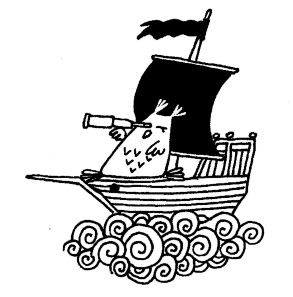
\includegraphics[scale=0.5]{22}}
\end{figure}
\end{SBSection*}

\end{song}

%\twocolumn
\begin{song}{Ленинградская (Все расстояния)}{}{Песни у костра}{Песни у костра}{}{}

\Ch{Am}{Все} расстоянья когда-нибудь в круг замы\Ch{E}{ка}ются,\par
\Ch{E}{Все} из разлук обязательно \Ch{E7}{встре}чей кон\Ch{Am}{ча}ются;\par
Должны про\Ch{Dm}{плыть} вокруг Зем\Ch{G}{ли,}\par
Вернуться в \Ch{C}{га}вань кораб\Ch{F}{ли,}\par   
Все поез\Ch{Dm}{да} в свои вер\Ch{E}{нуть}ся горо\Ch{Am}{да.}\\
 
Шумный вокзал то встречает друзей , то прощается,\par
Мы расстаемся, но снова назад возвращаемся -\par
Чтоб снова встать в огромный круг,\par
И снова знать, что рядом друг ,\par
И песни петь, чтоб больше не было разлук.\\
 
Все расстоянья когда-нибудь в круг замыкаются,\par
Все из разлук обязательно встречей кончаются;\par
И через год, и через пять,\par
Мы с вами встретимся опять,\par
Ничто не сможет нашей дружбе помешать.\par

\end{song}

%\twocolumn
\begin{song}{Десять капель}{}{Танцы Минус}{Танцы Минус}{}{}

Проигрыш: (2 раза)\par 
\Ch{C}{} \Ch{E}{} \Ch{Am}{} \Ch{F}{} \Ch{C}{} \Ch{E}{} \Ch{Am}{} \Ch{F}{}

\Ch{C}{Де}сять капель дож\Ch{E}{дя} у тебя на пле\Ch{Am}{че}\par
Ты забыла свой \Ch{F}{зонт,} ты спешила ко \Ch{C}{мне.}\par
Десять капель дож\Ch{E}{дя} на плече у те\Ch{Am}{бя,}\par
Десять капель люб\Ch{F}{ви,} десять капель ог\Ch{C}{ня}\\

Припев:\\(Три первых слова в припеве дублируются вторым голосом)\par
\tt\Ch{C}{Т}воя\Ch{E}{} ладо\Ch{Am}{нь} горит\Ch{F}{} в моих руках\par
\tt\Ch{C}{Л}юбви\Ch{E}{ }пож\Ch{Am}{ар} горит в тво\Ch{F}{их} глазах\\

Проигрыш.\\

Время делает шаг, время делает круг\par
Мы забудем друзей, мы забудем подруг\par
Просто выпьем вина из любви и огня\par
Десять капель меня, десять капель тебя\\

Припев.\\

Голос твой в тишине околдует меня\par
Ярким жарким огнем стану я до утра\par
Ты прикажешь гори, и я вспыхну любя\par
В этом пламени ты, в этом пламени я.\par

\end{song}

%\twocolumn
\begin{song}{Макет}{}{Песни у костра}{Сказка}{}{}
sadfsfthanks,\par
\begin{SBOpGroup}
asdas\
\end{SBOpGroup}
\begin{SBSection*}fdf\end{SBSection*}
\begin{SBVerse*}\end{SBVerse*}
\begin{SBChorus*}\end{SBChorus*}

\begin{SBOccurs}{23}
dsf
\end{SBOccurs}

\begin{SBSection*}
\begin{figure}[b!]
\center{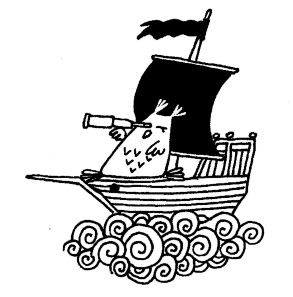
\includegraphics[scale=0.5]{22}}
\end{figure}
\end{SBSection*}
\end{song}

\mainmatter

\renewcommand{\footrulewidth}{0.0pt}
\renewcommand{\item}{\par\hangindent=40pt}
\renewcommand{\subitem}{\par\hangindent=40pt \hspace*{20pt}}
\renewcommand{\subsubitem}{\par\hangindent=40pt \hspace*{30pt}}

\newpage
\raggedright%\documentclass[a5paper,11pt]{book}
%\usepackage{fancyhdr}
%\usepackage[chordbk]{songbook}
%
%\usepackage[T2A]{fontenc}
%\usepackage[utf8]{inputenc}
%\usepackage[russian]{babel}
%
%\title{A Church Songbook}
%\author{}
%\date{Revised:  \RevDate}
%
%\newcommand{\RelDate}{13 November'19}
%\newcommand{\RevDate}{\today}

\documentclass[11pt,a5paper]{book}
\usepackage[a5paper]{geometry}
\usepackage[chordbk]{songbook}
\usepackage[T2A]{fontenc}
\usepackage[utf8]{inputenc}
\usepackage[russian]{babel}
\usepackage{cmap} % для работы поиска кириллицы в pdf

%\usepackage{amsmath,amsthm,amssymb}
%\usepackage{mathtext}


\usepackage[pdftex]{graphicx}
\usepackage{lscape}
%\usepackage{vmargin}
\usepackage{textcomp}
\usepackage{setspace}
%\usepackage{marvosym}
\usepackage{gensymb} %%%for \micro tag
\usepackage{upgreek} %%% \upmu
\usepackage{tipa}
\usepackage{phonetic}
%\usepackage[greek,english]{babel}
\usepackage{threeparttable}
\usepackage{multirow}
\usepackage{harvard}
\usepackage{longtable}
\renewcommand{\sectionmark}[1]{\markright{#1}}
\renewcommand{\chaptermark}[1]{\markboth{#1}{}}
\addto\captionsenglish{\renewcommand{\bibname}{References}}
\usepackage{latexsym,fancyhdr}

\newcommand{\RelDate}{26 Апреля'1984}
\newcommand{\RevDate}{\today}

%%%
% C.C.L.I. license number definition; for copyright licensing info.
% One of these macros will be manually inserted into the {CpyRt}
% parameter of the {song} environment.
%
%       \CCLInumber - The actual copyright license number.  Don't
%               insert this command in the {CpyRt} parameter, use one
%               of the others.
%       \CCLIed - Indicates a song falls under our CCLI license.
%       \NotCCLIed - Indicates a song doesn't fall under our CCLI
%               license.  Public Domain songs fall into this category.
%       \PGranted - We have received specific permission from the
%               copyright holder to use this song.
%       \PPending - We are in the process of obtaining permission to
%               use this song.
%%%
\newcommand{\CCLInumber}{Your CCLI Number}
\newcommand{\CCLIed}{{\CpyRtInfoFont (CCLI \CCLInumber)}}
\newcommand{\NotCCLIed}{\relax}
\newcommand{\PGranted}{\relax}
\newcommand{\PPending}{{\CpyRtInfoFont (Permission Pending)}}

%%%
% Title page information.
%%%
\title{ Сказочный песенник}
\author{}
\date{Созданно:  \RevDate}


%%%
% Define fonts to use in the headers and footers of the songbook.
%%%
\newcommand{\LHeadFont}{\normalsize}            % = cmr12  at 12pt
\newcommand{\CHeadFont}{\normalsize\rm}         % = cmr12  at 12pt
\newcommand{\RHeadFont}{\normalsize}            % = cmr12  at 12pt
\newcommand{\LFootFont}{\scriptsize}            % = cmr8   at  8pt
\newcommand{\CFootFont}{\tiny\myTinySF}         % = cmss8  at  8pt
\newcommand{\RFootFont}{\scriptsize}            % = cmr8   at  8pt

%%%
% Turn on and define fancy page heading/footing definition.
%%%
\pagestyle{fancy}

\ifChordBk
  % It's a words & chords songbook...
%  \addtolength{\headwidth}{\marginparsep}
%  \addtolength{\headwidth}{\marginparwidth}
  \renewcommand{\headrulewidth}{0.0pt}
  \renewcommand{\footrulewidth}{0.0pt}
%  \fancyhead[LE,RO]{\LHeadFont\emph{\leftmark\/}}
%  \fancyhead[CE,CO]{\CHeadFont\thepage}
  \fancyhead[RE,LO]{~}
\else\ifOverhead
  % It's an overhead...
  \renewcommand{\footrulewidth}{0pt}
  \renewcommand{\headrulewidth}{0pt}
  \fancyhead[LE,RO]{}
  \fancyhead[CE,CO]{}
  \fancyhead[RE,LO]{}
\else\ifWordBk
  % It's a words only songbook...
  \addtolength{\headwidth}{\marginparsep}
  \addtolength{\headwidth}{\marginparwidth}
  \renewcommand{\headrulewidth}{0.0pt}
  \renewcommand{\footrulewidth}{0.0pt}
  \fancyhead[LE,RO]{\LHeadFont A Church Songbook}
  \fancyhead[CE,CO]{\CHeadFont\thepage}
  \fancyhead[RE,LO]{\RHeadFont\RelDate}
\fi\fi\fi

%\fancyfoot[LE,RO]{\LFootFont Property of The Church}
%\ifSongEject
%  \fancyfoot[CE,CO]{\CFootFont \RevDate}
%\else
%  \fancyfoot[CE,CO]{\CFootFont}
%\fi
%\fancyfoot[RE,LO]{\RFootFont Material used by permission.}

%%%
% Turn on/off index-file generation.  Uncomment the \makeindex line to
% turn index generation on;  comment it out to turn index generation
% off.
%%%
\makeTitleIndex         %% Title and First Line Index.
\makeTitleContents      %% Table of Contents.
\makeKeyIndex           %% Index of song by key.
\graphicspath{{img/}} % папка с картинками
\DeclareGraphicsExtensions{.pdf,.png,.jpg} % форматы, которые будем считать картинками

%\newenvironment{song}[7][Y]{
%% Comment markers to negate
%\if#1Y\ExcludeSongfalse\else\ExcludeSongtrue\fi% the newline.
%\ifPrintAllSongs\ExcludeSongfalse\fi
%\SongMarkboth{\relax}{\relax}
%\SBinSongEnvtrue
%\renewcommand{\SBinSongEnv}{\True}
%\ifWordsOnly
%	\setlength{\parindent}{0pt}
%\fi

%%%
% Redefine fonts from SongBook style that I don't like.
%%%
\font\myTinySF=cmss8 at 8pt
\renewcommand{\CpyRtInfoFont}{\tiny\myTinySF}


%
%\font\myTinySF=cmss8    at  8pt
%\font\myHugeSF=cmssbx10 at 25pt
%\renewcommand{\CpyRtInfoFont}{\tiny\myTinySF}
%\newcommand{\myTitleFont}{\Huge\myHugeSF}
%\newcommand{\mySubTitleFont}{\large\sf}

%%% Работа с русским языком
%\usepackage[no-math]{fontspec}      %% подготавливает загрузку шрифтов Open Type, True Type и др.
%\defaultfontfeatures{Ligatures={TeX},Renderer=Basic}  %% свойства шрифтов по умолчанию
%\setmainfont[Ligatures={TeX,Historic}]{Times New Roman} %% задаёт основной шрифт документа
%\setsansfont{Helvetica Neue}                    %% задаёт шрифт без засечек

%\newfontfamily{\allods}{AllodsWest}

\newcommand{\SBPubDomm}{~}
\renewcommand{\CpyRt}[3][Y]{%
\if#1Y\begin{center}\fi
\if\blank{#2}%
\if\blank{#3}%
{\CpyRtFont\copyright \SBUnknownTag{} \CpyRtInfoFont}%
\else
{\CpyRtFont\copyright \SBUnknownTag{} \CpyRtInfoFont #3}%
\fi%
\else%
\ifthenelse{\equal{#2}{\SBPubDomm}}
{%then
{\CpyRtFont #2 \CpyRtInfoFont #3}%
}{%else
{\CpyRtFont #2 \CpyRtInfoFont #3}%
}%fi
\fi%
\if#1Y\end{center}\fi
}


\newcommand{\SBUnknownTagg}{~}
\renewcommand{\WAndM}[2][Y]{~}
\renewcommand{\WAndM}[2][Y]{%
\if#1Y\begin{center}\fi
\if\blank{#2}%
{\SBUnknownTagg}%
\else
{~}%
\fi
\if#1Y\end{center}\fi
}

\renewcommand{\STitle}[3][Y]{%
\setcounter{SBVerseCnt}{0}%
\setcounter{SBSectionCnt}{0}%
\ifExcludeSong\relax%
	\else\keyIndex{{\protect\sbChord#3\protect\relax} -- #2}{\theSBSongCnt}\fi%
	\vspace{\SpaceAboveSTitle}%
\if#1Y\begin{center}\fi
	{}{\STitleFont\LARGE #2}%
	\ifWordsOnly\relax\else\fi%
	\if#1Y\end{center}\fi
\STitleMarkboth{#2}{\relax}%
}


%\renewenvironment{SBOpGroup}{%
%	\sbSetsbBaselineSkipAmt%
%	\bgroup%
%	\begin{list}{\hbox{}}
%	  {\setlength {\leftmargin}
%		{\HangAmt}
%		\setlength{\itemindent}
%			{-\HangAmt}
%		\setlength{\listparindent}{-\HangAmt}
%		\setlength{\topsep}{0pt}
%		\setlength{\parsep}{0pt}
%		\setlength{\labelwidth}{0pt}
%		\setlength{\labelsep}{0pt}
%		\setlength{\baselineskip} {\sbBaselineSkipAmt}
%	}%\item}
%{\end{list}%
\newcommand{\SBChorusTagg}{Припев}
\renewenvironment{SBChorus}{%
\sbSetsbBaselineSkipAmt%
\bgroup%
\SBChorusMarkright{\SBChorusTag}
\begin{list}{{\SBChorusTagFont\SBChorusTagg}}
{\setlength {\leftmargin}
{\LeftMarginSBChorus + \HangAmt}
\setlength{\itemindent}
{-\HangAmt}
\setlength{\listparindent}{-\HangAmt}
\setlength{\parsep}
{0pt}
\setlength{\baselineskip} {\sbBaselineSkipAmt}
}%
\item}
{\end{list}%
\egroup%
\SpaceAfterChorus%
}

\renewcommand{\tt}{\indent \indent}
%\renewcommand{\nt}{\noindent}


\usepackage{amsmath}

\makeArtistIndex
\makeTitleIndex         %% Title and First Line Index.
\makeTitleContents      %% Table of Contents.
\makeKeyIndex           %% Index of song by key.
%\usepackage{printallsongs}

\begin{document} 
\maketitle

\mainmatter


\begin{song}{Вожатский гимн}{}{Сказка}{Сказка}{}{}

По \Ch{Am}{ла}герю подъём, нас горн зовёт!\par
Забудь о том, что ночь была бес\Ch{C}{сон}ною\par
Смо\Ch{Dm}{чи} водою \Ch{G}{ве}ки воспа\Ch{C}{лён}\Ch{F}{ные}\par    
По\Ch{Dm}{вя}зывай свой \Ch{E}{галс}тук — и впе\Ch{Am (A7)}{рёд!}\par
Смо\Ch{Dm}{чи} водою \Ch{G}{ве}ки воспа\Ch{C}{лён}\Ch{F}{ные}\par    
По\Ch{Dm}{вя}зывай свой \Ch{E}{галс}тук — и впе\Ch{Am (A7)}{рёд!}\par

%	\begin{SBChorus*}
\ttНе\Ch{E}{про}сто воспитывать \Ch{Am}{но}вых людей,\par
\ttНу \Ch{E}{что} ж, это наша с то\Ch{Am}{бою} свя\Ch{A7}{ты}ня.\par
\ttМой \Ch{Dm}{друг}, нам до\Ch{G}{ве}рили \Ch{C}{ду}ши де\Ch{F}{тей},\par
\ttИх \Ch{Dm}{ра}достный \Ch{Am}{смех} нам на\Ch{E}{гра}да от\Ch{Am}{ны}не.\par
\ttМой \Ch{Dm}{друг}, нам до\Ch{G}{ве}рили \Ch{C}{ду}ши де\Ch{F}{тей},\par
\ttИх \Ch{Dm}{ра}достный \Ch{Am}{смех} нам на\Ch{E}{гра}да от\Ch{Am}{ны}не.\\
%\end{SBChorus*}

Отбой, засыпает детвора.\par
Взгляни на их улыбки полусонные,\par
Пускай им снятся острова зелёные,\par
А нам опять работать до утра!\par
Пускай им снятся острова зелёные,\par
А нам опять работать до утра!\par

\tt И пусть от бессилья затихнешь не раз,\par
\ttИ голос усталый до хрипа натружен,\par
\ttПусть будут умней и счастливее нас\par
\ttТе дети, в которых вложили мы души!\par
\ttПусть будут умней и счастливее нас\par
\ttТе дети, в которых вложили мы души!

\end{song}

\begin{song}{Сказка в неглиже}{}{Сказка}{Сказка}{}{}

Есть у \Ch{C}{каж}дого добрая сказка в ду\Ch{F}{ше,}\par 
Надо \Ch{G}{толь}ко прочесть этой сказки стра\Ch{C}{ни}цы.\par
В тиши\Ch{C}{не}, разо\Ch{C7}{де}тая вся в негли\Ch{F}{же,}\par
Пусть на\Ch{G}{ве}ки она, пусть на\Ch{F}{ве}ки она сохра\Ch{C}{ни}тся. \Ch{C7}{ }\par 
В тиши\Ch{F}{не,} разо\Ch{G}{де}тая вся в негли\Ch{C}{же,} \Ch{Am}{}\par
Пусть на\Ch{F}{ве}ки она, пусть на\Ch{G}{ве}ки она сохра\Ch{C}{ни}тся.\\


\ttЭту сказку пред другом раскрыть поспеши,\par
\ttА врагу не спеши эту сказку поведать.\par
\ttПусть растут и читают ее малыши.\par
\ttБудь добрей, и тебя минут всякие беды.\par
\ttПусть растут и читают ее малыши.\par
\ttБудь добрей, и тебя минут всякие беды.\\


\Ch{C7}{}Будет \Ch{F}{мно}го распутий, \Ch{G}{до}рог и тре\Ch{C}{вог.}\Ch{Am}{}\par
На вис\Ch{F}{ки} твои ляжет \Ch{G}{не}тающий \Ch{C}{ин}ей, \Ch{C7}{}\par
И пой\Ch{F}{мёшь,} научившись чи\Ch{G}{тать} между \Ch{C}{строк:} \Ch{Am}{}\par
Даже \Ch{F}{гнус}ный злодей \Ch{G}{в} этой сказке не\Ch{C}{ви}нен. \Ch{C7}{}\par
И пой\Ch{F}{мёшь,} научившись чи\Ch{G}{тать} между ст\Ch{C}{рок:} \Ch{A}{}\par
Даже \Ch{F}{гнус}ный злодей \Ch{G}{в} этой сказке не\Ch{C}{ви}нен.\\

\Ch{C}{} \Ch{G}{} \Ch{F}{} \Ch{G}{} \Ch{C}{} \Ch{C7}{}\par
\Ch{C}{} \Ch{G}{} \Ch{F}{} \Ch{G}{} \Ch{C}{}
\end{song}

%\twocolumn
\begin{song}{Вожатский марш}{}{Сказка}{Сказка}{}{}

Есть на\Ch{Am}{род} у нас весёлый,\par
Самой \Ch{C}{луч}шей в мире пробы,\par
Песни \Ch{G}{петь} всегда мас\Ch{C}{так.}\Ch{A7}{}\par
Он всег\Ch{Dm}{да} всего добьётся,\par
Он Вожа\Ch{Am}{ты}ми зовётся,\par
\Ch{E}{Так} и только \Ch{Am (A7)}{так!}\par
Он всег\Ch{Dm}{да} всего добьётся,\par
Он Во\Ch{Am}{жа}тыми зовётся,\par
\Ch{E}{Так} и только \Ch{Am (A7)}{так!}\\

Домосед привязан к дому\par
И по случаю такому,\par
Он из дома — ни на шаг!\par
А вожатый — он в дороге,\par
Он готов в огонь и в воду,\par
Так и только так!\par
А вожатый — он в дороге,\par
Он готов в огонь и в воду,\par
Так и только так!\\
\newpage
Жадный денежки считает,\par
Все считает и считает,\par
К пятаку кладет пятак.\par
А вожатый деньги тратит,\par
Не боясь, что их не хватит,\par
Так и только так!\par
А вожатый деньги тратит,\par
Не боясь, что их не хватит,\par
Так и только так!\\

Холостяк в любовь не верит,\par
Все не верит и не верит,\par
Потому что холостяк.\par
А вожатых не влюблённых\par
Не найдёшь определённо,\par
Так и только так!\par
А вожатых не влюблённых\par
Не найдёшь определённо,\par
Так и только так!\par

\begin{SBSection*}
\begin{figure}[b!]
\center{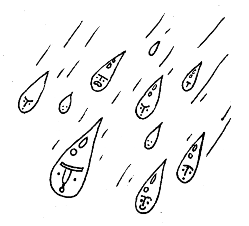
\includegraphics[scale=0.5]{16}}
\end{figure}
\end{SBSection*}
\end{song}

%\twocolumn
\begin{song}{Двадцать дней}{}{Сказка}{Сказка}{}{}


Двадцать дн\Ch{Dm}{ей} – это смена без дня.\par
“Маловато”,– вам скажут друзь\Ch{Gm}{я,}\par
А вожатый отв\Ch{C}{ет}ит люб\Ch{F}{ой}:\par
Это ср\Ch{Gm}{ок} очень д\Ch{A}{аж}е больш\Ch{Dm}{ой!}\\
 

Припев:\par
\ttМожно з\Ch{Gm C}{а-а-а-а} него усп\Ch{Dm}{ет}ь,\par
\ttНаприм\Ch{Gm}{ер,} полмилли\Ch{A}{он}а песен сп\Ch{Dm}{еть,}\par
\ttНо не к\Ch{Gm}{ажд}ый ведь поймет,\par
\ttКак так быстро раскрыв\Ch{A}{ат}ься может р\Ch{Dm}{от!}\\


Для полярника это не срок:\par
Не успеет просохнуть носок.\par
А вожатый успеет подряд \par
Вымыть, высушить сотню ребят!\\

Припев:\par
\ttВедь за смену, как за год \par
\ttСтолько разных мелочей произойдет,\par
\ttНо пока что нам везет,\par
\ttНас начальство для чего-то бережёт.\\


\newpage
Хоть и длинными кажутся дни,\par
Но как миг пролетели они.\par
Будешь долго потом вспоминать,\par
Как в отбой ты любил слово «СПАААТЬ!!!»\\

Припев:\par
\tt          	— Говорят за двадцать дней \par
\tt          	Все узнаешь о напарнице своей…\par
\tt          	— Только это ерунда,\par
\tt          	Обо всем ты не узнаешь никогда!\\

Смена вряд ли даст ответ:\par
Ты нашел свое призванье или нет.\par
Так что надо продолжать,\par
Двадцать раз по двадцать суток отсчитать!\\

\begin{SBSection*}
\begin{figure}[b!]
\center{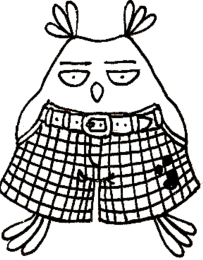
\includegraphics[scale=0.5]{17}}
\end{figure}
\end{SBSection*}

\end{song}

%\twocolumn
\begin{song}{Непогода}{}{Павел Смеян}{Павел Смеян}{}{}

\Ch{D}{Из}менения в природе \Ch{G}{пр}оисходят г\Ch{A}{од} от года,\par
\Ch{D}{Не}погода нынче в моде,\Ch{G}{} н\Ch{F#7}{епог}ода, непогода,\par
\Ch{}Hm{Слов}но из вод\Ch{F#7}{опро}вода \Ch{D7}{ль}ёт на нас с неб\Ch{G}{ес} во\Ch{Hm}{да…}\par
Полг\Ch{G}{од}а плох\Ch{A}{ая} пог\Ch{D}{од}а, \Ch{Hm}{пол}го\Ch{G}{да} — совс\Ch{A}{ем} нику\Ch{D}{да}.\par
Полг\Ch{G}{од}а плох\Ch{A}{ая} пог\Ch{D}{од}а, \Ch{Hm}{пол}го\Ch{G}{да} — сов\Ch{F#7}{сем} нику\Ch{Hm}{да.}\\


\SBChorusTagg:\par
\ttНикуда, нику\Ch{Em}{да н}ельз\Ch{A}{я} укр\Ch{D}{ы}ться н\Ch{Hm}{ам,}\par
\ttНо откладывать ж\Ch{Em}{изнь} ни\Ch{A}{как} нель\Ch{D}{зя}, \Ch{Hm}{}\par
\ttНикуда, нику\Ch{Em}{да, н}о зн\Ch{A}{ай}, что гд\Ch{D}{е}-то т\Ch{Hm}{ам}\par
\ttКто-то ищет теб\Ch{G}{я} сре\Ch{F#7}{ди д}ожд\Ch{Hm}{я.} \Ch{A}{}\\


Грома грозные раскаты от заката до восхода,\par
За грехи людские плата — непогода, непогода,\par
Не ангина, не простуда, посерьёзнее беда.\par
Полгода плохая погода, полгода — совсем никуда\par,
Полгода плохая погода, полгода — совсем никуда.\\\


\SBChorusTagg:\par
\ttНикуда, нику\Ch{Em}{да н}ельз\Ch{A}{я} укр\Ch{D}{ы}ться н\Ch{Hm}{ам,}\par
\ttНо откладывать ж\Ch{Em}{изнь} ни\Ch{A}{как} нель\Ch{D}{зя}, \Ch{Hm}{}\par
\ttНикуда, нику\Ch{Em}{да, н}о зн\Ch{A}{ай}, что гд\Ch{D}{е}-то т\Ch{Hm}{ам}\par
\ttКто-то ищет теб\Ch{G}{я} сре\Ch{F#7}{ди д}ожд\Ch{Hm}{я.} \Ch{A}{}\\


\end{song}

%\twocolumn
\begin{song}{Птенцы}{}{Сказка}{Сказка}{}{}

\Ch{Am}{}  \Ch{Am}{}

Как птенцы из гнез\Ch{Dm}{да} мы \Ch{E}{вы}па\Ch{Am}{ли.}\par
Ты не бойся при\Ch{Dm}{хо}да \Ch{G}{ве}че\Ch{C}{ра.}\par
Под та\Ch{A7}{ки}ми боль\Ch{F}{ши}ми \Ch{A7}{ли}па\Ch{Dm}{ми}\par
Нам с то\Ch{F}{бой} опа\Ch{Dm}{сать}ся \Ch{F}{не}\Ch{E}{че}\Ch{Am}{го.}\\
 
Под такими густыми звёздами -\par
Разве их не для нас рассыпали,\par
Мы не против гнездовья - просто мы\par
Из него ненароком выпали.\\

Это только вначале кажется,\par
Что без дома прожить нельзя никак,\par
Что важней пропитанья кашица,\par
Чем огромные звёзды на небе.\\

Ты не бойся ни тьмы, ни холода.\par
Будет день и найдётся пища нам,\par
Мы ещё пролетим над городом\par
На крыле до небес возвышенном.\\

Пролетим ещё - эка невидаль\par
Над Нью-Йорком, Парижем, Триполи\par
И над липой, откуда некогда,\par
Как птенцы из гнезда мы выпали.\\

Как птенцы из гнезда мы выпали.\par
Ты не бойся прихода вечера.\par
Под такими большими липами\par
Нам с тобой опасаться нечего.\\

\end{song}

%\twocolumn
\begin{song}{Продавец зонтиков}{}{Веня Дркин}{Веня Дркин}{}{}

\Ch{Am}{Город} этот выдумал о\Ch{Dm}{дин} художник,\par
\Ch{G}{Лю}ди в нем не знали, что та\Ch{C}{ко}е дождик.\par
\Ch{A7}{Про}сто не слыхали, что та\Ch{Dm}{ко}е зонтик –\par
\Ch{E7}{Вот} такие люди жили в \Ch{Am}{го}роде том.\par
И один чудак, в старый плащ одетый,\par
Продавал там зонтики зимой и летом,\par
Продавал там зонтики зимой и летом\par
И такую песенку он напевал:\\

\SBChorusTagg:\par
\tt“Господа, купите зонтик.\par
\ttБелый зонтик, красный зонтик,\par
\ttЖелтый зонтик, синий зонтик –\par
\ttМожет пригодится вам.”\\

Были домики у них из пластилина,\par
Из пустых коробочек автомашины,\par
И, не опасаясь никакой ангины,\par
Маленькие люди жили в городе том.\par
Маленькие были у людей заботы:\par
Шли они в кино или в театр с работы.\par
Вечером в подъезде целовался кто-то.\par
Все шутили и смеялись над стариком.\\


\SBChorusTagg.\\

\newpage

Маленькое небо как-то вдруг намокло,\par
В крошечных домишках задрожали стекла,\par
И огромный дождь пошел гулять по крышам,\par
Сразу все схватили насморк в городе том.\par
Вспомнили тут люди о торговце старом,\par
Кинулись искать его по всем базарам,\par
Но исчез торговец со своим товаром.\par
Только песенка осталась в память о нем:\\

\SBChorusTagg.\par

\begin{SBSection*}
\begin{figure}[b!]
\center{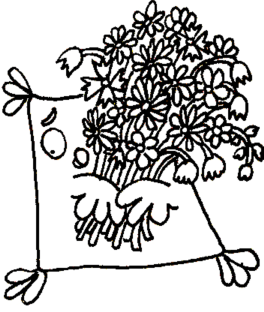
\includegraphics[scale=0.5]{15}}
\end{figure}
\end{SBSection*}

\end{song}

%\twocolumn
\begin{song}{Белая гвардия}{}{Белая гвардия}{Белая гвардия}{}{}

Проигрыш: (2 раза)\par 
\Ch{Am}{} \Ch{D}{} \Ch{G}{} \Ch{C}{} \Ch{Am}{} \Ch{H7}{} \Ch{Em}\\

\Ch{Em}{Белая} гвардия, белый снег,\par
\Ch{Am7}{Белая} музыка революций.\par
\Ch{D7}{Белая} женщина, нервный смех,\par
\Ch{G}{Белого} платья слегка коснуться.\par
 
Белой рукой распахнуть окно,\par
Белого света в нем не видя.\par
Белое выпить до дна вино,\par
В красную улицу в белом выйти.\\

Припев:\par
\ttКог\Ch{Em}{да} ты вернешься,\par
\ttВсе будет и\Ch{Am}{на}че, и нам бы узнать друг друга,\par
\ttКог\Ch{D7}{да} ты вернешься,\par
\ttА я не же\Ch{G}{на} и даже \Ch{H7}{не} подруга.\par
\ttКог\Ch{C}{да} ты вернешься,\par
\ttКо мне, так без\Ch{Am}{ум}но тебя любившей в прошлом,\par
\tt\Ch{D7}{Ко}гда ты вернешься -\par
\ttУвидишь, что ж\Ch{G}{ре}бий давно и не \Ch{E7}{нами} брошен.\\

Проигрыш.\\
 
\newpage
Сизые сумерки прошлых лет\par
Робко крадутся по переулкам.\par
В этом окне еле брезжит свет,\par
Ноты истрепаны, звуки гулки.\par
Тонкие пальцы срывают аккорд...\par
Нам не простят безрассудного дара.\par
Бьются в решетку стальных ворот\par
Пять океанов земного шара.\\

Припев. \par
Проигрыш.\\
 
Красный трамвай простучал в ночи,\par
Красный закат догорел в бокале,\par
Красные-красные кумачи\par
С красных деревьев на землю упали.\par
Я не ждала тебя в октябре,\par
Виделись сны, я листала сонник:\par
Красные лошади на заре\par
Били копытами о подоконник.\\

Припев:\par
\ttКогда ты вернешься,\par
\ttВсе будет иначе, и нам бы узнать друг друга,\par
\ttКогда ты вернешься,\par
\ttА я не жена и даже не подруга.\par
\ttКогда ты вернешься,\par
\ttВернешься в наш город обетованный,\par
\ttКогда ты вернешься -\par
\ttТакой невозможный и такой желанный?\\

Проигрыш.\par

\end{song}

%\twocolumn
\begin{song}{Перевал}{}{Песни у костра}{Песни у костра}{}{}


\Ch{Am}{Про}сто нечего нам \Ch{Dm}{боль}ше терять\par
\Ch{E}{Всё} нам вспомнится на \Ch{Am}{Страшном} суде.\par
Эта ночь легла, как \Ch{Dm}{тот} перевал,\par
\Ch{G}{За} которым испол\Ch{C}{нень}е надежд.\par
\Ch{A7}{Про}сто прожитое—про\Ch{Dm}{жи}то зря, \Ch{G}{}\par
Но не в этом, пони\Ch{C}{мае}шь ли, соль… \Ch{Am}{}\par
Слышишь, падают дож\Ch{Dm}{ди} октября.\par
\Ch{E}{Ви}дишь, старый дом сто\Ch{Am}{ит} средь лесов.\\

Мы затопим в доме печь, в доме печь,\par
Мы гитару позовем со стены.\par
Просто нечего нам больше беречь,\par
Ведь за нами все мосты сожжены.\par
Все мосты, все перекрёстки дорог,\par
Все прошёптанные тайны в ночи.\par
Каждый сделал все, что смог, все, что смог,\par
Мы об этом помолчим, помолчим.\\


И луна взойдет заплывшей свечой,\par
Ставни скрипнут  на ветру, на ветру.\par
Ах, как я тебя люблю горячо,\par
Это годы не сотрут, не сотрут.\par
Мы оставшихся друзей соберем,\par
Мы набьем картошкой старый рюкзак,\par
Люди спросят: "Что за шум, что за гам?"\par
Мы ответим: "Просто так,  просто так”...\\

\newpage

    Просто так идут дожди в октябре,\par
    И потеряны от счастья ключи.\par
    Это всё, конечно, мне, конечно, мне,\par
    Но об этом помолчим, помолчим.\par
    Просто прожитое—прожито зря,\par
    Но не в этом, понимаешь ли, соль…\par
    Слышишь, падают дожди октября.\par
    Видишь, старый дом стоит средь лесов.\par


\begin{SBSection*}
\begin{figure}[b!]
\center{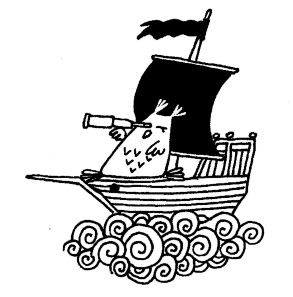
\includegraphics[scale=0.5]{22}}
\end{figure}
\end{SBSection*}

\end{song}

%\twocolumn
\begin{song}{Ленинградская (Все расстояния)}{}{Песни у костра}{Песни у костра}{}{}

\Ch{Am}{Все} расстоянья когда-нибудь в круг замы\Ch{E}{ка}ются,\par
\Ch{E}{Все} из разлук обязательно \Ch{E7}{встре}чей кон\Ch{Am}{ча}ются;\par
Должны про\Ch{Dm}{плыть} вокруг Зем\Ch{G}{ли,}\par
Вернуться в \Ch{C}{га}вань кораб\Ch{F}{ли,}\par   
Все поез\Ch{Dm}{да} в свои вер\Ch{E}{нуть}ся горо\Ch{Am}{да.}\\
 
Шумный вокзал то встречает друзей , то прощается,\par
Мы расстаемся, но снова назад возвращаемся -\par
Чтоб снова встать в огромный круг,\par
И снова знать, что рядом друг ,\par
И песни петь, чтоб больше не было разлук.\\
 
Все расстоянья когда-нибудь в круг замыкаются,\par
Все из разлук обязательно встречей кончаются;\par
И через год, и через пять,\par
Мы с вами встретимся опять,\par
Ничто не сможет нашей дружбе помешать.\par

\end{song}

%\twocolumn
\begin{song}{Десять капель}{}{Танцы Минус}{Танцы Минус}{}{}

Проигрыш: (2 раза)\par 
\Ch{C}{} \Ch{E}{} \Ch{Am}{} \Ch{F}{} \Ch{C}{} \Ch{E}{} \Ch{Am}{} \Ch{F}{}

\Ch{C}{Де}сять капель дож\Ch{E}{дя} у тебя на пле\Ch{Am}{че}\par
Ты забыла свой \Ch{F}{зонт,} ты спешила ко \Ch{C}{мне.}\par
Десять капель дож\Ch{E}{дя} на плече у те\Ch{Am}{бя,}\par
Десять капель люб\Ch{F}{ви,} десять капель ог\Ch{C}{ня}\\

Припев:\\(Три первых слова в припеве дублируются вторым голосом)\par
\tt\Ch{C}{Т}воя\Ch{E}{} ладо\Ch{Am}{нь} горит\Ch{F}{} в моих руках\par
\tt\Ch{C}{Л}юбви\Ch{E}{ }пож\Ch{Am}{ар} горит в тво\Ch{F}{их} глазах\\

Проигрыш.\\

Время делает шаг, время делает круг\par
Мы забудем друзей, мы забудем подруг\par
Просто выпьем вина из любви и огня\par
Десять капель меня, десять капель тебя\\

Припев.\\

Голос твой в тишине околдует меня\par
Ярким жарким огнем стану я до утра\par
Ты прикажешь гори, и я вспыхну любя\par
В этом пламени ты, в этом пламени я.\par

\end{song}

%\twocolumn
\begin{song}{Макет}{}{Песни у костра}{Сказка}{}{}
sadfsfthanks,\par
\begin{SBOpGroup}
asdas\
\end{SBOpGroup}
\begin{SBSection*}fdf\end{SBSection*}
\begin{SBVerse*}\end{SBVerse*}
\begin{SBChorus*}\end{SBChorus*}

\begin{SBOccurs}{23}
dsf
\end{SBOccurs}

\begin{SBSection*}
\begin{figure}[b!]
\center{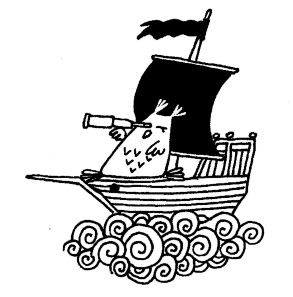
\includegraphics[scale=0.5]{22}}
\end{figure}
\end{SBSection*}
\end{song}

\mainmatter

\renewcommand{\footrulewidth}{0.0pt}
\renewcommand{\item}{\par\hangindent=40pt}
\renewcommand{\subitem}{\par\hangindent=40pt \hspace*{20pt}}
\renewcommand{\subsubitem}{\par\hangindent=40pt \hspace*{30pt}}

\newpage
\raggedright\input{/home/p_a/git/ska3ka/ps.adx}

\centering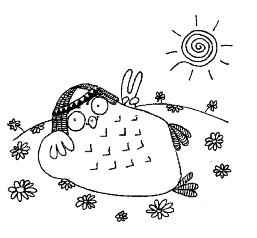
\includegraphics[scale=0.5]{10}

\newpage
\raggedright\input{/home/p_a/git/ska3ka/ps.tdx}

\centering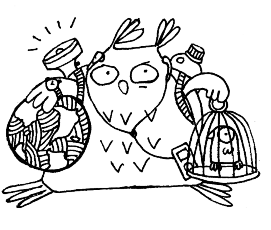
\includegraphics[scale=0.5]{11}

\end{document}


\centering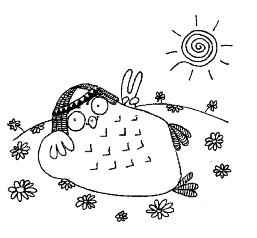
\includegraphics[scale=0.5]{10}

\newpage
\raggedright%\documentclass[a5paper,11pt]{book}
%\usepackage{fancyhdr}
%\usepackage[chordbk]{songbook}
%
%\usepackage[T2A]{fontenc}
%\usepackage[utf8]{inputenc}
%\usepackage[russian]{babel}
%
%\title{A Church Songbook}
%\author{}
%\date{Revised:  \RevDate}
%
%\newcommand{\RelDate}{13 November'19}
%\newcommand{\RevDate}{\today}

\documentclass[11pt,a5paper]{book}
\usepackage[a5paper]{geometry}
\usepackage[chordbk]{songbook}
\usepackage[T2A]{fontenc}
\usepackage[utf8]{inputenc}
\usepackage[russian]{babel}
\usepackage{cmap} % для работы поиска кириллицы в pdf

%\usepackage{amsmath,amsthm,amssymb}
%\usepackage{mathtext}


\usepackage[pdftex]{graphicx}
\usepackage{lscape}
%\usepackage{vmargin}
\usepackage{textcomp}
\usepackage{setspace}
%\usepackage{marvosym}
\usepackage{gensymb} %%%for \micro tag
\usepackage{upgreek} %%% \upmu
\usepackage{tipa}
\usepackage{phonetic}
%\usepackage[greek,english]{babel}
\usepackage{threeparttable}
\usepackage{multirow}
\usepackage{harvard}
\usepackage{longtable}
\renewcommand{\sectionmark}[1]{\markright{#1}}
\renewcommand{\chaptermark}[1]{\markboth{#1}{}}
\addto\captionsenglish{\renewcommand{\bibname}{References}}
\usepackage{latexsym,fancyhdr}

\newcommand{\RelDate}{26 Апреля'1984}
\newcommand{\RevDate}{\today}

%%%
% C.C.L.I. license number definition; for copyright licensing info.
% One of these macros will be manually inserted into the {CpyRt}
% parameter of the {song} environment.
%
%       \CCLInumber - The actual copyright license number.  Don't
%               insert this command in the {CpyRt} parameter, use one
%               of the others.
%       \CCLIed - Indicates a song falls under our CCLI license.
%       \NotCCLIed - Indicates a song doesn't fall under our CCLI
%               license.  Public Domain songs fall into this category.
%       \PGranted - We have received specific permission from the
%               copyright holder to use this song.
%       \PPending - We are in the process of obtaining permission to
%               use this song.
%%%
\newcommand{\CCLInumber}{Your CCLI Number}
\newcommand{\CCLIed}{{\CpyRtInfoFont (CCLI \CCLInumber)}}
\newcommand{\NotCCLIed}{\relax}
\newcommand{\PGranted}{\relax}
\newcommand{\PPending}{{\CpyRtInfoFont (Permission Pending)}}

%%%
% Title page information.
%%%
\title{ Сказочный песенник}
\author{}
\date{Созданно:  \RevDate}


%%%
% Define fonts to use in the headers and footers of the songbook.
%%%
\newcommand{\LHeadFont}{\normalsize}            % = cmr12  at 12pt
\newcommand{\CHeadFont}{\normalsize\rm}         % = cmr12  at 12pt
\newcommand{\RHeadFont}{\normalsize}            % = cmr12  at 12pt
\newcommand{\LFootFont}{\scriptsize}            % = cmr8   at  8pt
\newcommand{\CFootFont}{\tiny\myTinySF}         % = cmss8  at  8pt
\newcommand{\RFootFont}{\scriptsize}            % = cmr8   at  8pt

%%%
% Turn on and define fancy page heading/footing definition.
%%%
\pagestyle{fancy}

\ifChordBk
  % It's a words & chords songbook...
%  \addtolength{\headwidth}{\marginparsep}
%  \addtolength{\headwidth}{\marginparwidth}
  \renewcommand{\headrulewidth}{0.0pt}
  \renewcommand{\footrulewidth}{0.0pt}
%  \fancyhead[LE,RO]{\LHeadFont\emph{\leftmark\/}}
%  \fancyhead[CE,CO]{\CHeadFont\thepage}
  \fancyhead[RE,LO]{~}
\else\ifOverhead
  % It's an overhead...
  \renewcommand{\footrulewidth}{0pt}
  \renewcommand{\headrulewidth}{0pt}
  \fancyhead[LE,RO]{}
  \fancyhead[CE,CO]{}
  \fancyhead[RE,LO]{}
\else\ifWordBk
  % It's a words only songbook...
  \addtolength{\headwidth}{\marginparsep}
  \addtolength{\headwidth}{\marginparwidth}
  \renewcommand{\headrulewidth}{0.0pt}
  \renewcommand{\footrulewidth}{0.0pt}
  \fancyhead[LE,RO]{\LHeadFont A Church Songbook}
  \fancyhead[CE,CO]{\CHeadFont\thepage}
  \fancyhead[RE,LO]{\RHeadFont\RelDate}
\fi\fi\fi

%\fancyfoot[LE,RO]{\LFootFont Property of The Church}
%\ifSongEject
%  \fancyfoot[CE,CO]{\CFootFont \RevDate}
%\else
%  \fancyfoot[CE,CO]{\CFootFont}
%\fi
%\fancyfoot[RE,LO]{\RFootFont Material used by permission.}

%%%
% Turn on/off index-file generation.  Uncomment the \makeindex line to
% turn index generation on;  comment it out to turn index generation
% off.
%%%
\makeTitleIndex         %% Title and First Line Index.
\makeTitleContents      %% Table of Contents.
\makeKeyIndex           %% Index of song by key.
\graphicspath{{img/}} % папка с картинками
\DeclareGraphicsExtensions{.pdf,.png,.jpg} % форматы, которые будем считать картинками

%\newenvironment{song}[7][Y]{
%% Comment markers to negate
%\if#1Y\ExcludeSongfalse\else\ExcludeSongtrue\fi% the newline.
%\ifPrintAllSongs\ExcludeSongfalse\fi
%\SongMarkboth{\relax}{\relax}
%\SBinSongEnvtrue
%\renewcommand{\SBinSongEnv}{\True}
%\ifWordsOnly
%	\setlength{\parindent}{0pt}
%\fi

%%%
% Redefine fonts from SongBook style that I don't like.
%%%
\font\myTinySF=cmss8 at 8pt
\renewcommand{\CpyRtInfoFont}{\tiny\myTinySF}


%
%\font\myTinySF=cmss8    at  8pt
%\font\myHugeSF=cmssbx10 at 25pt
%\renewcommand{\CpyRtInfoFont}{\tiny\myTinySF}
%\newcommand{\myTitleFont}{\Huge\myHugeSF}
%\newcommand{\mySubTitleFont}{\large\sf}

%%% Работа с русским языком
%\usepackage[no-math]{fontspec}      %% подготавливает загрузку шрифтов Open Type, True Type и др.
%\defaultfontfeatures{Ligatures={TeX},Renderer=Basic}  %% свойства шрифтов по умолчанию
%\setmainfont[Ligatures={TeX,Historic}]{Times New Roman} %% задаёт основной шрифт документа
%\setsansfont{Helvetica Neue}                    %% задаёт шрифт без засечек

%\newfontfamily{\allods}{AllodsWest}

\newcommand{\SBPubDomm}{~}
\renewcommand{\CpyRt}[3][Y]{%
\if#1Y\begin{center}\fi
\if\blank{#2}%
\if\blank{#3}%
{\CpyRtFont\copyright \SBUnknownTag{} \CpyRtInfoFont}%
\else
{\CpyRtFont\copyright \SBUnknownTag{} \CpyRtInfoFont #3}%
\fi%
\else%
\ifthenelse{\equal{#2}{\SBPubDomm}}
{%then
{\CpyRtFont #2 \CpyRtInfoFont #3}%
}{%else
{\CpyRtFont #2 \CpyRtInfoFont #3}%
}%fi
\fi%
\if#1Y\end{center}\fi
}


\newcommand{\SBUnknownTagg}{~}
\renewcommand{\WAndM}[2][Y]{~}
\renewcommand{\WAndM}[2][Y]{%
\if#1Y\begin{center}\fi
\if\blank{#2}%
{\SBUnknownTagg}%
\else
{~}%
\fi
\if#1Y\end{center}\fi
}

\renewcommand{\STitle}[3][Y]{%
\setcounter{SBVerseCnt}{0}%
\setcounter{SBSectionCnt}{0}%
\ifExcludeSong\relax%
	\else\keyIndex{{\protect\sbChord#3\protect\relax} -- #2}{\theSBSongCnt}\fi%
	\vspace{\SpaceAboveSTitle}%
\if#1Y\begin{center}\fi
	{}{\STitleFont\LARGE #2}%
	\ifWordsOnly\relax\else\fi%
	\if#1Y\end{center}\fi
\STitleMarkboth{#2}{\relax}%
}


%\renewenvironment{SBOpGroup}{%
%	\sbSetsbBaselineSkipAmt%
%	\bgroup%
%	\begin{list}{\hbox{}}
%	  {\setlength {\leftmargin}
%		{\HangAmt}
%		\setlength{\itemindent}
%			{-\HangAmt}
%		\setlength{\listparindent}{-\HangAmt}
%		\setlength{\topsep}{0pt}
%		\setlength{\parsep}{0pt}
%		\setlength{\labelwidth}{0pt}
%		\setlength{\labelsep}{0pt}
%		\setlength{\baselineskip} {\sbBaselineSkipAmt}
%	}%\item}
%{\end{list}%
\newcommand{\SBChorusTagg}{Припев}
\renewenvironment{SBChorus}{%
\sbSetsbBaselineSkipAmt%
\bgroup%
\SBChorusMarkright{\SBChorusTag}
\begin{list}{{\SBChorusTagFont\SBChorusTagg}}
{\setlength {\leftmargin}
{\LeftMarginSBChorus + \HangAmt}
\setlength{\itemindent}
{-\HangAmt}
\setlength{\listparindent}{-\HangAmt}
\setlength{\parsep}
{0pt}
\setlength{\baselineskip} {\sbBaselineSkipAmt}
}%
\item}
{\end{list}%
\egroup%
\SpaceAfterChorus%
}

\renewcommand{\tt}{\indent \indent}
%\renewcommand{\nt}{\noindent}


\usepackage{amsmath}

\makeArtistIndex
\makeTitleIndex         %% Title and First Line Index.
\makeTitleContents      %% Table of Contents.
\makeKeyIndex           %% Index of song by key.
%\usepackage{printallsongs}

\begin{document} 
\maketitle

\mainmatter


\begin{song}{Вожатский гимн}{}{Сказка}{Сказка}{}{}

По \Ch{Am}{ла}герю подъём, нас горн зовёт!\par
Забудь о том, что ночь была бес\Ch{C}{сон}ною\par
Смо\Ch{Dm}{чи} водою \Ch{G}{ве}ки воспа\Ch{C}{лён}\Ch{F}{ные}\par    
По\Ch{Dm}{вя}зывай свой \Ch{E}{галс}тук — и впе\Ch{Am (A7)}{рёд!}\par
Смо\Ch{Dm}{чи} водою \Ch{G}{ве}ки воспа\Ch{C}{лён}\Ch{F}{ные}\par    
По\Ch{Dm}{вя}зывай свой \Ch{E}{галс}тук — и впе\Ch{Am (A7)}{рёд!}\par

%	\begin{SBChorus*}
\ttНе\Ch{E}{про}сто воспитывать \Ch{Am}{но}вых людей,\par
\ttНу \Ch{E}{что} ж, это наша с то\Ch{Am}{бою} свя\Ch{A7}{ты}ня.\par
\ttМой \Ch{Dm}{друг}, нам до\Ch{G}{ве}рили \Ch{C}{ду}ши де\Ch{F}{тей},\par
\ttИх \Ch{Dm}{ра}достный \Ch{Am}{смех} нам на\Ch{E}{гра}да от\Ch{Am}{ны}не.\par
\ttМой \Ch{Dm}{друг}, нам до\Ch{G}{ве}рили \Ch{C}{ду}ши де\Ch{F}{тей},\par
\ttИх \Ch{Dm}{ра}достный \Ch{Am}{смех} нам на\Ch{E}{гра}да от\Ch{Am}{ны}не.\\
%\end{SBChorus*}

Отбой, засыпает детвора.\par
Взгляни на их улыбки полусонные,\par
Пускай им снятся острова зелёные,\par
А нам опять работать до утра!\par
Пускай им снятся острова зелёные,\par
А нам опять работать до утра!\par

\tt И пусть от бессилья затихнешь не раз,\par
\ttИ голос усталый до хрипа натружен,\par
\ttПусть будут умней и счастливее нас\par
\ttТе дети, в которых вложили мы души!\par
\ttПусть будут умней и счастливее нас\par
\ttТе дети, в которых вложили мы души!

\end{song}

\begin{song}{Сказка в неглиже}{}{Сказка}{Сказка}{}{}

Есть у \Ch{C}{каж}дого добрая сказка в ду\Ch{F}{ше,}\par 
Надо \Ch{G}{толь}ко прочесть этой сказки стра\Ch{C}{ни}цы.\par
В тиши\Ch{C}{не}, разо\Ch{C7}{де}тая вся в негли\Ch{F}{же,}\par
Пусть на\Ch{G}{ве}ки она, пусть на\Ch{F}{ве}ки она сохра\Ch{C}{ни}тся. \Ch{C7}{ }\par 
В тиши\Ch{F}{не,} разо\Ch{G}{де}тая вся в негли\Ch{C}{же,} \Ch{Am}{}\par
Пусть на\Ch{F}{ве}ки она, пусть на\Ch{G}{ве}ки она сохра\Ch{C}{ни}тся.\\


\ttЭту сказку пред другом раскрыть поспеши,\par
\ttА врагу не спеши эту сказку поведать.\par
\ttПусть растут и читают ее малыши.\par
\ttБудь добрей, и тебя минут всякие беды.\par
\ttПусть растут и читают ее малыши.\par
\ttБудь добрей, и тебя минут всякие беды.\\


\Ch{C7}{}Будет \Ch{F}{мно}го распутий, \Ch{G}{до}рог и тре\Ch{C}{вог.}\Ch{Am}{}\par
На вис\Ch{F}{ки} твои ляжет \Ch{G}{не}тающий \Ch{C}{ин}ей, \Ch{C7}{}\par
И пой\Ch{F}{мёшь,} научившись чи\Ch{G}{тать} между \Ch{C}{строк:} \Ch{Am}{}\par
Даже \Ch{F}{гнус}ный злодей \Ch{G}{в} этой сказке не\Ch{C}{ви}нен. \Ch{C7}{}\par
И пой\Ch{F}{мёшь,} научившись чи\Ch{G}{тать} между ст\Ch{C}{рок:} \Ch{A}{}\par
Даже \Ch{F}{гнус}ный злодей \Ch{G}{в} этой сказке не\Ch{C}{ви}нен.\\

\Ch{C}{} \Ch{G}{} \Ch{F}{} \Ch{G}{} \Ch{C}{} \Ch{C7}{}\par
\Ch{C}{} \Ch{G}{} \Ch{F}{} \Ch{G}{} \Ch{C}{}
\end{song}

%\twocolumn
\begin{song}{Вожатский марш}{}{Сказка}{Сказка}{}{}

Есть на\Ch{Am}{род} у нас весёлый,\par
Самой \Ch{C}{луч}шей в мире пробы,\par
Песни \Ch{G}{петь} всегда мас\Ch{C}{так.}\Ch{A7}{}\par
Он всег\Ch{Dm}{да} всего добьётся,\par
Он Вожа\Ch{Am}{ты}ми зовётся,\par
\Ch{E}{Так} и только \Ch{Am (A7)}{так!}\par
Он всег\Ch{Dm}{да} всего добьётся,\par
Он Во\Ch{Am}{жа}тыми зовётся,\par
\Ch{E}{Так} и только \Ch{Am (A7)}{так!}\\

Домосед привязан к дому\par
И по случаю такому,\par
Он из дома — ни на шаг!\par
А вожатый — он в дороге,\par
Он готов в огонь и в воду,\par
Так и только так!\par
А вожатый — он в дороге,\par
Он готов в огонь и в воду,\par
Так и только так!\\
\newpage
Жадный денежки считает,\par
Все считает и считает,\par
К пятаку кладет пятак.\par
А вожатый деньги тратит,\par
Не боясь, что их не хватит,\par
Так и только так!\par
А вожатый деньги тратит,\par
Не боясь, что их не хватит,\par
Так и только так!\\

Холостяк в любовь не верит,\par
Все не верит и не верит,\par
Потому что холостяк.\par
А вожатых не влюблённых\par
Не найдёшь определённо,\par
Так и только так!\par
А вожатых не влюблённых\par
Не найдёшь определённо,\par
Так и только так!\par

\begin{SBSection*}
\begin{figure}[b!]
\center{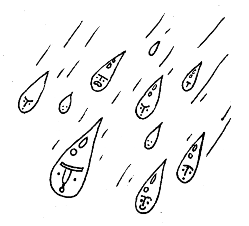
\includegraphics[scale=0.5]{16}}
\end{figure}
\end{SBSection*}
\end{song}

%\twocolumn
\begin{song}{Двадцать дней}{}{Сказка}{Сказка}{}{}


Двадцать дн\Ch{Dm}{ей} – это смена без дня.\par
“Маловато”,– вам скажут друзь\Ch{Gm}{я,}\par
А вожатый отв\Ch{C}{ет}ит люб\Ch{F}{ой}:\par
Это ср\Ch{Gm}{ок} очень д\Ch{A}{аж}е больш\Ch{Dm}{ой!}\\
 

Припев:\par
\ttМожно з\Ch{Gm C}{а-а-а-а} него усп\Ch{Dm}{ет}ь,\par
\ttНаприм\Ch{Gm}{ер,} полмилли\Ch{A}{он}а песен сп\Ch{Dm}{еть,}\par
\ttНо не к\Ch{Gm}{ажд}ый ведь поймет,\par
\ttКак так быстро раскрыв\Ch{A}{ат}ься может р\Ch{Dm}{от!}\\


Для полярника это не срок:\par
Не успеет просохнуть носок.\par
А вожатый успеет подряд \par
Вымыть, высушить сотню ребят!\\

Припев:\par
\ttВедь за смену, как за год \par
\ttСтолько разных мелочей произойдет,\par
\ttНо пока что нам везет,\par
\ttНас начальство для чего-то бережёт.\\


\newpage
Хоть и длинными кажутся дни,\par
Но как миг пролетели они.\par
Будешь долго потом вспоминать,\par
Как в отбой ты любил слово «СПАААТЬ!!!»\\

Припев:\par
\tt          	— Говорят за двадцать дней \par
\tt          	Все узнаешь о напарнице своей…\par
\tt          	— Только это ерунда,\par
\tt          	Обо всем ты не узнаешь никогда!\\

Смена вряд ли даст ответ:\par
Ты нашел свое призванье или нет.\par
Так что надо продолжать,\par
Двадцать раз по двадцать суток отсчитать!\\

\begin{SBSection*}
\begin{figure}[b!]
\center{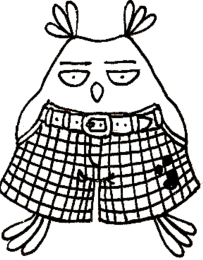
\includegraphics[scale=0.5]{17}}
\end{figure}
\end{SBSection*}

\end{song}

%\twocolumn
\begin{song}{Непогода}{}{Павел Смеян}{Павел Смеян}{}{}

\Ch{D}{Из}менения в природе \Ch{G}{пр}оисходят г\Ch{A}{од} от года,\par
\Ch{D}{Не}погода нынче в моде,\Ch{G}{} н\Ch{F#7}{епог}ода, непогода,\par
\Ch{}Hm{Слов}но из вод\Ch{F#7}{опро}вода \Ch{D7}{ль}ёт на нас с неб\Ch{G}{ес} во\Ch{Hm}{да…}\par
Полг\Ch{G}{од}а плох\Ch{A}{ая} пог\Ch{D}{од}а, \Ch{Hm}{пол}го\Ch{G}{да} — совс\Ch{A}{ем} нику\Ch{D}{да}.\par
Полг\Ch{G}{од}а плох\Ch{A}{ая} пог\Ch{D}{од}а, \Ch{Hm}{пол}го\Ch{G}{да} — сов\Ch{F#7}{сем} нику\Ch{Hm}{да.}\\


\SBChorusTagg:\par
\ttНикуда, нику\Ch{Em}{да н}ельз\Ch{A}{я} укр\Ch{D}{ы}ться н\Ch{Hm}{ам,}\par
\ttНо откладывать ж\Ch{Em}{изнь} ни\Ch{A}{как} нель\Ch{D}{зя}, \Ch{Hm}{}\par
\ttНикуда, нику\Ch{Em}{да, н}о зн\Ch{A}{ай}, что гд\Ch{D}{е}-то т\Ch{Hm}{ам}\par
\ttКто-то ищет теб\Ch{G}{я} сре\Ch{F#7}{ди д}ожд\Ch{Hm}{я.} \Ch{A}{}\\


Грома грозные раскаты от заката до восхода,\par
За грехи людские плата — непогода, непогода,\par
Не ангина, не простуда, посерьёзнее беда.\par
Полгода плохая погода, полгода — совсем никуда\par,
Полгода плохая погода, полгода — совсем никуда.\\\


\SBChorusTagg:\par
\ttНикуда, нику\Ch{Em}{да н}ельз\Ch{A}{я} укр\Ch{D}{ы}ться н\Ch{Hm}{ам,}\par
\ttНо откладывать ж\Ch{Em}{изнь} ни\Ch{A}{как} нель\Ch{D}{зя}, \Ch{Hm}{}\par
\ttНикуда, нику\Ch{Em}{да, н}о зн\Ch{A}{ай}, что гд\Ch{D}{е}-то т\Ch{Hm}{ам}\par
\ttКто-то ищет теб\Ch{G}{я} сре\Ch{F#7}{ди д}ожд\Ch{Hm}{я.} \Ch{A}{}\\


\end{song}

%\twocolumn
\begin{song}{Птенцы}{}{Сказка}{Сказка}{}{}

\Ch{Am}{}  \Ch{Am}{}

Как птенцы из гнез\Ch{Dm}{да} мы \Ch{E}{вы}па\Ch{Am}{ли.}\par
Ты не бойся при\Ch{Dm}{хо}да \Ch{G}{ве}че\Ch{C}{ра.}\par
Под та\Ch{A7}{ки}ми боль\Ch{F}{ши}ми \Ch{A7}{ли}па\Ch{Dm}{ми}\par
Нам с то\Ch{F}{бой} опа\Ch{Dm}{сать}ся \Ch{F}{не}\Ch{E}{че}\Ch{Am}{го.}\\
 
Под такими густыми звёздами -\par
Разве их не для нас рассыпали,\par
Мы не против гнездовья - просто мы\par
Из него ненароком выпали.\\

Это только вначале кажется,\par
Что без дома прожить нельзя никак,\par
Что важней пропитанья кашица,\par
Чем огромные звёзды на небе.\\

Ты не бойся ни тьмы, ни холода.\par
Будет день и найдётся пища нам,\par
Мы ещё пролетим над городом\par
На крыле до небес возвышенном.\\

Пролетим ещё - эка невидаль\par
Над Нью-Йорком, Парижем, Триполи\par
И над липой, откуда некогда,\par
Как птенцы из гнезда мы выпали.\\

Как птенцы из гнезда мы выпали.\par
Ты не бойся прихода вечера.\par
Под такими большими липами\par
Нам с тобой опасаться нечего.\\

\end{song}

%\twocolumn
\begin{song}{Продавец зонтиков}{}{Веня Дркин}{Веня Дркин}{}{}

\Ch{Am}{Город} этот выдумал о\Ch{Dm}{дин} художник,\par
\Ch{G}{Лю}ди в нем не знали, что та\Ch{C}{ко}е дождик.\par
\Ch{A7}{Про}сто не слыхали, что та\Ch{Dm}{ко}е зонтик –\par
\Ch{E7}{Вот} такие люди жили в \Ch{Am}{го}роде том.\par
И один чудак, в старый плащ одетый,\par
Продавал там зонтики зимой и летом,\par
Продавал там зонтики зимой и летом\par
И такую песенку он напевал:\\

\SBChorusTagg:\par
\tt“Господа, купите зонтик.\par
\ttБелый зонтик, красный зонтик,\par
\ttЖелтый зонтик, синий зонтик –\par
\ttМожет пригодится вам.”\\

Были домики у них из пластилина,\par
Из пустых коробочек автомашины,\par
И, не опасаясь никакой ангины,\par
Маленькие люди жили в городе том.\par
Маленькие были у людей заботы:\par
Шли они в кино или в театр с работы.\par
Вечером в подъезде целовался кто-то.\par
Все шутили и смеялись над стариком.\\


\SBChorusTagg.\\

\newpage

Маленькое небо как-то вдруг намокло,\par
В крошечных домишках задрожали стекла,\par
И огромный дождь пошел гулять по крышам,\par
Сразу все схватили насморк в городе том.\par
Вспомнили тут люди о торговце старом,\par
Кинулись искать его по всем базарам,\par
Но исчез торговец со своим товаром.\par
Только песенка осталась в память о нем:\\

\SBChorusTagg.\par

\begin{SBSection*}
\begin{figure}[b!]
\center{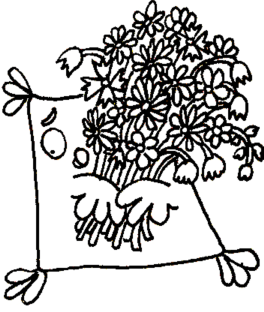
\includegraphics[scale=0.5]{15}}
\end{figure}
\end{SBSection*}

\end{song}

%\twocolumn
\begin{song}{Белая гвардия}{}{Белая гвардия}{Белая гвардия}{}{}

Проигрыш: (2 раза)\par 
\Ch{Am}{} \Ch{D}{} \Ch{G}{} \Ch{C}{} \Ch{Am}{} \Ch{H7}{} \Ch{Em}\\

\Ch{Em}{Белая} гвардия, белый снег,\par
\Ch{Am7}{Белая} музыка революций.\par
\Ch{D7}{Белая} женщина, нервный смех,\par
\Ch{G}{Белого} платья слегка коснуться.\par
 
Белой рукой распахнуть окно,\par
Белого света в нем не видя.\par
Белое выпить до дна вино,\par
В красную улицу в белом выйти.\\

Припев:\par
\ttКог\Ch{Em}{да} ты вернешься,\par
\ttВсе будет и\Ch{Am}{на}че, и нам бы узнать друг друга,\par
\ttКог\Ch{D7}{да} ты вернешься,\par
\ttА я не же\Ch{G}{на} и даже \Ch{H7}{не} подруга.\par
\ttКог\Ch{C}{да} ты вернешься,\par
\ttКо мне, так без\Ch{Am}{ум}но тебя любившей в прошлом,\par
\tt\Ch{D7}{Ко}гда ты вернешься -\par
\ttУвидишь, что ж\Ch{G}{ре}бий давно и не \Ch{E7}{нами} брошен.\\

Проигрыш.\\
 
\newpage
Сизые сумерки прошлых лет\par
Робко крадутся по переулкам.\par
В этом окне еле брезжит свет,\par
Ноты истрепаны, звуки гулки.\par
Тонкие пальцы срывают аккорд...\par
Нам не простят безрассудного дара.\par
Бьются в решетку стальных ворот\par
Пять океанов земного шара.\\

Припев. \par
Проигрыш.\\
 
Красный трамвай простучал в ночи,\par
Красный закат догорел в бокале,\par
Красные-красные кумачи\par
С красных деревьев на землю упали.\par
Я не ждала тебя в октябре,\par
Виделись сны, я листала сонник:\par
Красные лошади на заре\par
Били копытами о подоконник.\\

Припев:\par
\ttКогда ты вернешься,\par
\ttВсе будет иначе, и нам бы узнать друг друга,\par
\ttКогда ты вернешься,\par
\ttА я не жена и даже не подруга.\par
\ttКогда ты вернешься,\par
\ttВернешься в наш город обетованный,\par
\ttКогда ты вернешься -\par
\ttТакой невозможный и такой желанный?\\

Проигрыш.\par

\end{song}

%\twocolumn
\begin{song}{Перевал}{}{Песни у костра}{Песни у костра}{}{}


\Ch{Am}{Про}сто нечего нам \Ch{Dm}{боль}ше терять\par
\Ch{E}{Всё} нам вспомнится на \Ch{Am}{Страшном} суде.\par
Эта ночь легла, как \Ch{Dm}{тот} перевал,\par
\Ch{G}{За} которым испол\Ch{C}{нень}е надежд.\par
\Ch{A7}{Про}сто прожитое—про\Ch{Dm}{жи}то зря, \Ch{G}{}\par
Но не в этом, пони\Ch{C}{мае}шь ли, соль… \Ch{Am}{}\par
Слышишь, падают дож\Ch{Dm}{ди} октября.\par
\Ch{E}{Ви}дишь, старый дом сто\Ch{Am}{ит} средь лесов.\\

Мы затопим в доме печь, в доме печь,\par
Мы гитару позовем со стены.\par
Просто нечего нам больше беречь,\par
Ведь за нами все мосты сожжены.\par
Все мосты, все перекрёстки дорог,\par
Все прошёптанные тайны в ночи.\par
Каждый сделал все, что смог, все, что смог,\par
Мы об этом помолчим, помолчим.\\


И луна взойдет заплывшей свечой,\par
Ставни скрипнут  на ветру, на ветру.\par
Ах, как я тебя люблю горячо,\par
Это годы не сотрут, не сотрут.\par
Мы оставшихся друзей соберем,\par
Мы набьем картошкой старый рюкзак,\par
Люди спросят: "Что за шум, что за гам?"\par
Мы ответим: "Просто так,  просто так”...\\

\newpage

    Просто так идут дожди в октябре,\par
    И потеряны от счастья ключи.\par
    Это всё, конечно, мне, конечно, мне,\par
    Но об этом помолчим, помолчим.\par
    Просто прожитое—прожито зря,\par
    Но не в этом, понимаешь ли, соль…\par
    Слышишь, падают дожди октября.\par
    Видишь, старый дом стоит средь лесов.\par


\begin{SBSection*}
\begin{figure}[b!]
\center{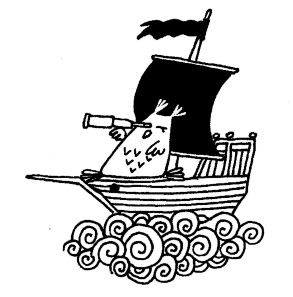
\includegraphics[scale=0.5]{22}}
\end{figure}
\end{SBSection*}

\end{song}

%\twocolumn
\begin{song}{Ленинградская (Все расстояния)}{}{Песни у костра}{Песни у костра}{}{}

\Ch{Am}{Все} расстоянья когда-нибудь в круг замы\Ch{E}{ка}ются,\par
\Ch{E}{Все} из разлук обязательно \Ch{E7}{встре}чей кон\Ch{Am}{ча}ются;\par
Должны про\Ch{Dm}{плыть} вокруг Зем\Ch{G}{ли,}\par
Вернуться в \Ch{C}{га}вань кораб\Ch{F}{ли,}\par   
Все поез\Ch{Dm}{да} в свои вер\Ch{E}{нуть}ся горо\Ch{Am}{да.}\\
 
Шумный вокзал то встречает друзей , то прощается,\par
Мы расстаемся, но снова назад возвращаемся -\par
Чтоб снова встать в огромный круг,\par
И снова знать, что рядом друг ,\par
И песни петь, чтоб больше не было разлук.\\
 
Все расстоянья когда-нибудь в круг замыкаются,\par
Все из разлук обязательно встречей кончаются;\par
И через год, и через пять,\par
Мы с вами встретимся опять,\par
Ничто не сможет нашей дружбе помешать.\par

\end{song}

%\twocolumn
\begin{song}{Десять капель}{}{Танцы Минус}{Танцы Минус}{}{}

Проигрыш: (2 раза)\par 
\Ch{C}{} \Ch{E}{} \Ch{Am}{} \Ch{F}{} \Ch{C}{} \Ch{E}{} \Ch{Am}{} \Ch{F}{}

\Ch{C}{Де}сять капель дож\Ch{E}{дя} у тебя на пле\Ch{Am}{че}\par
Ты забыла свой \Ch{F}{зонт,} ты спешила ко \Ch{C}{мне.}\par
Десять капель дож\Ch{E}{дя} на плече у те\Ch{Am}{бя,}\par
Десять капель люб\Ch{F}{ви,} десять капель ог\Ch{C}{ня}\\

Припев:\\(Три первых слова в припеве дублируются вторым голосом)\par
\tt\Ch{C}{Т}воя\Ch{E}{} ладо\Ch{Am}{нь} горит\Ch{F}{} в моих руках\par
\tt\Ch{C}{Л}юбви\Ch{E}{ }пож\Ch{Am}{ар} горит в тво\Ch{F}{их} глазах\\

Проигрыш.\\

Время делает шаг, время делает круг\par
Мы забудем друзей, мы забудем подруг\par
Просто выпьем вина из любви и огня\par
Десять капель меня, десять капель тебя\\

Припев.\\

Голос твой в тишине околдует меня\par
Ярким жарким огнем стану я до утра\par
Ты прикажешь гори, и я вспыхну любя\par
В этом пламени ты, в этом пламени я.\par

\end{song}

%\twocolumn
\begin{song}{Макет}{}{Песни у костра}{Сказка}{}{}
sadfsfthanks,\par
\begin{SBOpGroup}
asdas\
\end{SBOpGroup}
\begin{SBSection*}fdf\end{SBSection*}
\begin{SBVerse*}\end{SBVerse*}
\begin{SBChorus*}\end{SBChorus*}

\begin{SBOccurs}{23}
dsf
\end{SBOccurs}

\begin{SBSection*}
\begin{figure}[b!]
\center{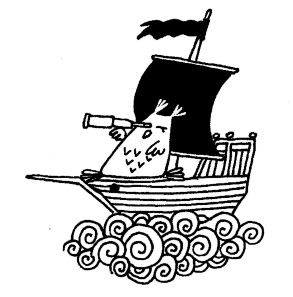
\includegraphics[scale=0.5]{22}}
\end{figure}
\end{SBSection*}
\end{song}

\mainmatter

\renewcommand{\footrulewidth}{0.0pt}
\renewcommand{\item}{\par\hangindent=40pt}
\renewcommand{\subitem}{\par\hangindent=40pt \hspace*{20pt}}
\renewcommand{\subsubitem}{\par\hangindent=40pt \hspace*{30pt}}

\newpage
\raggedright\input{/home/p_a/git/ska3ka/ps.adx}

\centering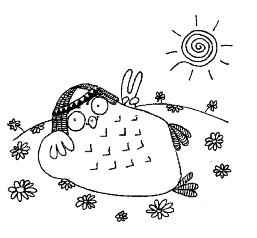
\includegraphics[scale=0.5]{10}

\newpage
\raggedright\input{/home/p_a/git/ska3ka/ps.tdx}

\centering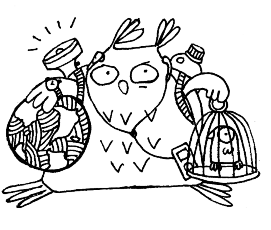
\includegraphics[scale=0.5]{11}

\end{document}


\centering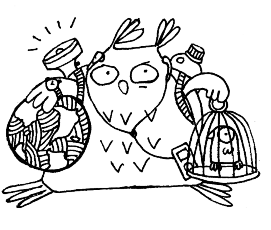
\includegraphics[scale=0.5]{11}

\end{document}


\centering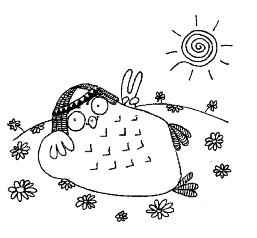
\includegraphics[scale=0.5]{10}

\newpage
\raggedright%\documentclass[a5paper,11pt]{book}
%\usepackage{fancyhdr}
%\usepackage[chordbk]{songbook}
%
%\usepackage[T2A]{fontenc}
%\usepackage[utf8]{inputenc}
%\usepackage[russian]{babel}
%
%\title{A Church Songbook}
%\author{}
%\date{Revised:  \RevDate}
%
%\newcommand{\RelDate}{13 November'19}
%\newcommand{\RevDate}{\today}

\documentclass[11pt,a5paper]{book}
\usepackage[a5paper]{geometry}
\usepackage[chordbk]{songbook}
\usepackage[T2A]{fontenc}
\usepackage[utf8]{inputenc}
\usepackage[russian]{babel}
\usepackage{cmap} % для работы поиска кириллицы в pdf

%\usepackage{amsmath,amsthm,amssymb}
%\usepackage{mathtext}


\usepackage[pdftex]{graphicx}
\usepackage{lscape}
%\usepackage{vmargin}
\usepackage{textcomp}
\usepackage{setspace}
%\usepackage{marvosym}
\usepackage{gensymb} %%%for \micro tag
\usepackage{upgreek} %%% \upmu
\usepackage{tipa}
\usepackage{phonetic}
%\usepackage[greek,english]{babel}
\usepackage{threeparttable}
\usepackage{multirow}
\usepackage{harvard}
\usepackage{longtable}
\renewcommand{\sectionmark}[1]{\markright{#1}}
\renewcommand{\chaptermark}[1]{\markboth{#1}{}}
\addto\captionsenglish{\renewcommand{\bibname}{References}}
\usepackage{latexsym,fancyhdr}

\newcommand{\RelDate}{26 Апреля'1984}
\newcommand{\RevDate}{\today}

%%%
% C.C.L.I. license number definition; for copyright licensing info.
% One of these macros will be manually inserted into the {CpyRt}
% parameter of the {song} environment.
%
%       \CCLInumber - The actual copyright license number.  Don't
%               insert this command in the {CpyRt} parameter, use one
%               of the others.
%       \CCLIed - Indicates a song falls under our CCLI license.
%       \NotCCLIed - Indicates a song doesn't fall under our CCLI
%               license.  Public Domain songs fall into this category.
%       \PGranted - We have received specific permission from the
%               copyright holder to use this song.
%       \PPending - We are in the process of obtaining permission to
%               use this song.
%%%
\newcommand{\CCLInumber}{Your CCLI Number}
\newcommand{\CCLIed}{{\CpyRtInfoFont (CCLI \CCLInumber)}}
\newcommand{\NotCCLIed}{\relax}
\newcommand{\PGranted}{\relax}
\newcommand{\PPending}{{\CpyRtInfoFont (Permission Pending)}}

%%%
% Title page information.
%%%
\title{ Сказочный песенник}
\author{}
\date{Созданно:  \RevDate}


%%%
% Define fonts to use in the headers and footers of the songbook.
%%%
\newcommand{\LHeadFont}{\normalsize}            % = cmr12  at 12pt
\newcommand{\CHeadFont}{\normalsize\rm}         % = cmr12  at 12pt
\newcommand{\RHeadFont}{\normalsize}            % = cmr12  at 12pt
\newcommand{\LFootFont}{\scriptsize}            % = cmr8   at  8pt
\newcommand{\CFootFont}{\tiny\myTinySF}         % = cmss8  at  8pt
\newcommand{\RFootFont}{\scriptsize}            % = cmr8   at  8pt

%%%
% Turn on and define fancy page heading/footing definition.
%%%
\pagestyle{fancy}

\ifChordBk
  % It's a words & chords songbook...
%  \addtolength{\headwidth}{\marginparsep}
%  \addtolength{\headwidth}{\marginparwidth}
  \renewcommand{\headrulewidth}{0.0pt}
  \renewcommand{\footrulewidth}{0.0pt}
%  \fancyhead[LE,RO]{\LHeadFont\emph{\leftmark\/}}
%  \fancyhead[CE,CO]{\CHeadFont\thepage}
  \fancyhead[RE,LO]{~}
\else\ifOverhead
  % It's an overhead...
  \renewcommand{\footrulewidth}{0pt}
  \renewcommand{\headrulewidth}{0pt}
  \fancyhead[LE,RO]{}
  \fancyhead[CE,CO]{}
  \fancyhead[RE,LO]{}
\else\ifWordBk
  % It's a words only songbook...
  \addtolength{\headwidth}{\marginparsep}
  \addtolength{\headwidth}{\marginparwidth}
  \renewcommand{\headrulewidth}{0.0pt}
  \renewcommand{\footrulewidth}{0.0pt}
  \fancyhead[LE,RO]{\LHeadFont A Church Songbook}
  \fancyhead[CE,CO]{\CHeadFont\thepage}
  \fancyhead[RE,LO]{\RHeadFont\RelDate}
\fi\fi\fi

%\fancyfoot[LE,RO]{\LFootFont Property of The Church}
%\ifSongEject
%  \fancyfoot[CE,CO]{\CFootFont \RevDate}
%\else
%  \fancyfoot[CE,CO]{\CFootFont}
%\fi
%\fancyfoot[RE,LO]{\RFootFont Material used by permission.}

%%%
% Turn on/off index-file generation.  Uncomment the \makeindex line to
% turn index generation on;  comment it out to turn index generation
% off.
%%%
\makeTitleIndex         %% Title and First Line Index.
\makeTitleContents      %% Table of Contents.
\makeKeyIndex           %% Index of song by key.
\graphicspath{{img/}} % папка с картинками
\DeclareGraphicsExtensions{.pdf,.png,.jpg} % форматы, которые будем считать картинками

%\newenvironment{song}[7][Y]{
%% Comment markers to negate
%\if#1Y\ExcludeSongfalse\else\ExcludeSongtrue\fi% the newline.
%\ifPrintAllSongs\ExcludeSongfalse\fi
%\SongMarkboth{\relax}{\relax}
%\SBinSongEnvtrue
%\renewcommand{\SBinSongEnv}{\True}
%\ifWordsOnly
%	\setlength{\parindent}{0pt}
%\fi

%%%
% Redefine fonts from SongBook style that I don't like.
%%%
\font\myTinySF=cmss8 at 8pt
\renewcommand{\CpyRtInfoFont}{\tiny\myTinySF}


%
%\font\myTinySF=cmss8    at  8pt
%\font\myHugeSF=cmssbx10 at 25pt
%\renewcommand{\CpyRtInfoFont}{\tiny\myTinySF}
%\newcommand{\myTitleFont}{\Huge\myHugeSF}
%\newcommand{\mySubTitleFont}{\large\sf}

%%% Работа с русским языком
%\usepackage[no-math]{fontspec}      %% подготавливает загрузку шрифтов Open Type, True Type и др.
%\defaultfontfeatures{Ligatures={TeX},Renderer=Basic}  %% свойства шрифтов по умолчанию
%\setmainfont[Ligatures={TeX,Historic}]{Times New Roman} %% задаёт основной шрифт документа
%\setsansfont{Helvetica Neue}                    %% задаёт шрифт без засечек

%\newfontfamily{\allods}{AllodsWest}

\newcommand{\SBPubDomm}{~}
\renewcommand{\CpyRt}[3][Y]{%
\if#1Y\begin{center}\fi
\if\blank{#2}%
\if\blank{#3}%
{\CpyRtFont\copyright \SBUnknownTag{} \CpyRtInfoFont}%
\else
{\CpyRtFont\copyright \SBUnknownTag{} \CpyRtInfoFont #3}%
\fi%
\else%
\ifthenelse{\equal{#2}{\SBPubDomm}}
{%then
{\CpyRtFont #2 \CpyRtInfoFont #3}%
}{%else
{\CpyRtFont #2 \CpyRtInfoFont #3}%
}%fi
\fi%
\if#1Y\end{center}\fi
}


\newcommand{\SBUnknownTagg}{~}
\renewcommand{\WAndM}[2][Y]{~}
\renewcommand{\WAndM}[2][Y]{%
\if#1Y\begin{center}\fi
\if\blank{#2}%
{\SBUnknownTagg}%
\else
{~}%
\fi
\if#1Y\end{center}\fi
}

\renewcommand{\STitle}[3][Y]{%
\setcounter{SBVerseCnt}{0}%
\setcounter{SBSectionCnt}{0}%
\ifExcludeSong\relax%
	\else\keyIndex{{\protect\sbChord#3\protect\relax} -- #2}{\theSBSongCnt}\fi%
	\vspace{\SpaceAboveSTitle}%
\if#1Y\begin{center}\fi
	{}{\STitleFont\LARGE #2}%
	\ifWordsOnly\relax\else\fi%
	\if#1Y\end{center}\fi
\STitleMarkboth{#2}{\relax}%
}


%\renewenvironment{SBOpGroup}{%
%	\sbSetsbBaselineSkipAmt%
%	\bgroup%
%	\begin{list}{\hbox{}}
%	  {\setlength {\leftmargin}
%		{\HangAmt}
%		\setlength{\itemindent}
%			{-\HangAmt}
%		\setlength{\listparindent}{-\HangAmt}
%		\setlength{\topsep}{0pt}
%		\setlength{\parsep}{0pt}
%		\setlength{\labelwidth}{0pt}
%		\setlength{\labelsep}{0pt}
%		\setlength{\baselineskip} {\sbBaselineSkipAmt}
%	}%\item}
%{\end{list}%
\newcommand{\SBChorusTagg}{Припев}
\renewenvironment{SBChorus}{%
\sbSetsbBaselineSkipAmt%
\bgroup%
\SBChorusMarkright{\SBChorusTag}
\begin{list}{{\SBChorusTagFont\SBChorusTagg}}
{\setlength {\leftmargin}
{\LeftMarginSBChorus + \HangAmt}
\setlength{\itemindent}
{-\HangAmt}
\setlength{\listparindent}{-\HangAmt}
\setlength{\parsep}
{0pt}
\setlength{\baselineskip} {\sbBaselineSkipAmt}
}%
\item}
{\end{list}%
\egroup%
\SpaceAfterChorus%
}

\renewcommand{\tt}{\indent \indent}
%\renewcommand{\nt}{\noindent}


\usepackage{amsmath}

\makeArtistIndex
\makeTitleIndex         %% Title and First Line Index.
\makeTitleContents      %% Table of Contents.
\makeKeyIndex           %% Index of song by key.
%\usepackage{printallsongs}

\begin{document} 
\maketitle

\mainmatter


\begin{song}{Вожатский гимн}{}{Сказка}{Сказка}{}{}

По \Ch{Am}{ла}герю подъём, нас горн зовёт!\par
Забудь о том, что ночь была бес\Ch{C}{сон}ною\par
Смо\Ch{Dm}{чи} водою \Ch{G}{ве}ки воспа\Ch{C}{лён}\Ch{F}{ные}\par    
По\Ch{Dm}{вя}зывай свой \Ch{E}{галс}тук — и впе\Ch{Am (A7)}{рёд!}\par
Смо\Ch{Dm}{чи} водою \Ch{G}{ве}ки воспа\Ch{C}{лён}\Ch{F}{ные}\par    
По\Ch{Dm}{вя}зывай свой \Ch{E}{галс}тук — и впе\Ch{Am (A7)}{рёд!}\par

%	\begin{SBChorus*}
\ttНе\Ch{E}{про}сто воспитывать \Ch{Am}{но}вых людей,\par
\ttНу \Ch{E}{что} ж, это наша с то\Ch{Am}{бою} свя\Ch{A7}{ты}ня.\par
\ttМой \Ch{Dm}{друг}, нам до\Ch{G}{ве}рили \Ch{C}{ду}ши де\Ch{F}{тей},\par
\ttИх \Ch{Dm}{ра}достный \Ch{Am}{смех} нам на\Ch{E}{гра}да от\Ch{Am}{ны}не.\par
\ttМой \Ch{Dm}{друг}, нам до\Ch{G}{ве}рили \Ch{C}{ду}ши де\Ch{F}{тей},\par
\ttИх \Ch{Dm}{ра}достный \Ch{Am}{смех} нам на\Ch{E}{гра}да от\Ch{Am}{ны}не.\\
%\end{SBChorus*}

Отбой, засыпает детвора.\par
Взгляни на их улыбки полусонные,\par
Пускай им снятся острова зелёные,\par
А нам опять работать до утра!\par
Пускай им снятся острова зелёные,\par
А нам опять работать до утра!\par

\tt И пусть от бессилья затихнешь не раз,\par
\ttИ голос усталый до хрипа натружен,\par
\ttПусть будут умней и счастливее нас\par
\ttТе дети, в которых вложили мы души!\par
\ttПусть будут умней и счастливее нас\par
\ttТе дети, в которых вложили мы души!

\end{song}

\begin{song}{Сказка в неглиже}{}{Сказка}{Сказка}{}{}

Есть у \Ch{C}{каж}дого добрая сказка в ду\Ch{F}{ше,}\par 
Надо \Ch{G}{толь}ко прочесть этой сказки стра\Ch{C}{ни}цы.\par
В тиши\Ch{C}{не}, разо\Ch{C7}{де}тая вся в негли\Ch{F}{же,}\par
Пусть на\Ch{G}{ве}ки она, пусть на\Ch{F}{ве}ки она сохра\Ch{C}{ни}тся. \Ch{C7}{ }\par 
В тиши\Ch{F}{не,} разо\Ch{G}{де}тая вся в негли\Ch{C}{же,} \Ch{Am}{}\par
Пусть на\Ch{F}{ве}ки она, пусть на\Ch{G}{ве}ки она сохра\Ch{C}{ни}тся.\\


\ttЭту сказку пред другом раскрыть поспеши,\par
\ttА врагу не спеши эту сказку поведать.\par
\ttПусть растут и читают ее малыши.\par
\ttБудь добрей, и тебя минут всякие беды.\par
\ttПусть растут и читают ее малыши.\par
\ttБудь добрей, и тебя минут всякие беды.\\


\Ch{C7}{}Будет \Ch{F}{мно}го распутий, \Ch{G}{до}рог и тре\Ch{C}{вог.}\Ch{Am}{}\par
На вис\Ch{F}{ки} твои ляжет \Ch{G}{не}тающий \Ch{C}{ин}ей, \Ch{C7}{}\par
И пой\Ch{F}{мёшь,} научившись чи\Ch{G}{тать} между \Ch{C}{строк:} \Ch{Am}{}\par
Даже \Ch{F}{гнус}ный злодей \Ch{G}{в} этой сказке не\Ch{C}{ви}нен. \Ch{C7}{}\par
И пой\Ch{F}{мёшь,} научившись чи\Ch{G}{тать} между ст\Ch{C}{рок:} \Ch{A}{}\par
Даже \Ch{F}{гнус}ный злодей \Ch{G}{в} этой сказке не\Ch{C}{ви}нен.\\

\Ch{C}{} \Ch{G}{} \Ch{F}{} \Ch{G}{} \Ch{C}{} \Ch{C7}{}\par
\Ch{C}{} \Ch{G}{} \Ch{F}{} \Ch{G}{} \Ch{C}{}
\end{song}

%\twocolumn
\begin{song}{Вожатский марш}{}{Сказка}{Сказка}{}{}

Есть на\Ch{Am}{род} у нас весёлый,\par
Самой \Ch{C}{луч}шей в мире пробы,\par
Песни \Ch{G}{петь} всегда мас\Ch{C}{так.}\Ch{A7}{}\par
Он всег\Ch{Dm}{да} всего добьётся,\par
Он Вожа\Ch{Am}{ты}ми зовётся,\par
\Ch{E}{Так} и только \Ch{Am (A7)}{так!}\par
Он всег\Ch{Dm}{да} всего добьётся,\par
Он Во\Ch{Am}{жа}тыми зовётся,\par
\Ch{E}{Так} и только \Ch{Am (A7)}{так!}\\

Домосед привязан к дому\par
И по случаю такому,\par
Он из дома — ни на шаг!\par
А вожатый — он в дороге,\par
Он готов в огонь и в воду,\par
Так и только так!\par
А вожатый — он в дороге,\par
Он готов в огонь и в воду,\par
Так и только так!\\
\newpage
Жадный денежки считает,\par
Все считает и считает,\par
К пятаку кладет пятак.\par
А вожатый деньги тратит,\par
Не боясь, что их не хватит,\par
Так и только так!\par
А вожатый деньги тратит,\par
Не боясь, что их не хватит,\par
Так и только так!\\

Холостяк в любовь не верит,\par
Все не верит и не верит,\par
Потому что холостяк.\par
А вожатых не влюблённых\par
Не найдёшь определённо,\par
Так и только так!\par
А вожатых не влюблённых\par
Не найдёшь определённо,\par
Так и только так!\par

\begin{SBSection*}
\begin{figure}[b!]
\center{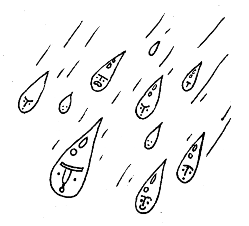
\includegraphics[scale=0.5]{16}}
\end{figure}
\end{SBSection*}
\end{song}

%\twocolumn
\begin{song}{Двадцать дней}{}{Сказка}{Сказка}{}{}


Двадцать дн\Ch{Dm}{ей} – это смена без дня.\par
“Маловато”,– вам скажут друзь\Ch{Gm}{я,}\par
А вожатый отв\Ch{C}{ет}ит люб\Ch{F}{ой}:\par
Это ср\Ch{Gm}{ок} очень д\Ch{A}{аж}е больш\Ch{Dm}{ой!}\\
 

Припев:\par
\ttМожно з\Ch{Gm C}{а-а-а-а} него усп\Ch{Dm}{ет}ь,\par
\ttНаприм\Ch{Gm}{ер,} полмилли\Ch{A}{он}а песен сп\Ch{Dm}{еть,}\par
\ttНо не к\Ch{Gm}{ажд}ый ведь поймет,\par
\ttКак так быстро раскрыв\Ch{A}{ат}ься может р\Ch{Dm}{от!}\\


Для полярника это не срок:\par
Не успеет просохнуть носок.\par
А вожатый успеет подряд \par
Вымыть, высушить сотню ребят!\\

Припев:\par
\ttВедь за смену, как за год \par
\ttСтолько разных мелочей произойдет,\par
\ttНо пока что нам везет,\par
\ttНас начальство для чего-то бережёт.\\


\newpage
Хоть и длинными кажутся дни,\par
Но как миг пролетели они.\par
Будешь долго потом вспоминать,\par
Как в отбой ты любил слово «СПАААТЬ!!!»\\

Припев:\par
\tt          	— Говорят за двадцать дней \par
\tt          	Все узнаешь о напарнице своей…\par
\tt          	— Только это ерунда,\par
\tt          	Обо всем ты не узнаешь никогда!\\

Смена вряд ли даст ответ:\par
Ты нашел свое призванье или нет.\par
Так что надо продолжать,\par
Двадцать раз по двадцать суток отсчитать!\\

\begin{SBSection*}
\begin{figure}[b!]
\center{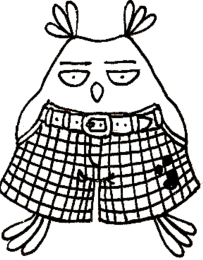
\includegraphics[scale=0.5]{17}}
\end{figure}
\end{SBSection*}

\end{song}

%\twocolumn
\begin{song}{Непогода}{}{Павел Смеян}{Павел Смеян}{}{}

\Ch{D}{Из}менения в природе \Ch{G}{пр}оисходят г\Ch{A}{од} от года,\par
\Ch{D}{Не}погода нынче в моде,\Ch{G}{} н\Ch{F#7}{епог}ода, непогода,\par
\Ch{}Hm{Слов}но из вод\Ch{F#7}{опро}вода \Ch{D7}{ль}ёт на нас с неб\Ch{G}{ес} во\Ch{Hm}{да…}\par
Полг\Ch{G}{од}а плох\Ch{A}{ая} пог\Ch{D}{од}а, \Ch{Hm}{пол}го\Ch{G}{да} — совс\Ch{A}{ем} нику\Ch{D}{да}.\par
Полг\Ch{G}{од}а плох\Ch{A}{ая} пог\Ch{D}{од}а, \Ch{Hm}{пол}го\Ch{G}{да} — сов\Ch{F#7}{сем} нику\Ch{Hm}{да.}\\


\SBChorusTagg:\par
\ttНикуда, нику\Ch{Em}{да н}ельз\Ch{A}{я} укр\Ch{D}{ы}ться н\Ch{Hm}{ам,}\par
\ttНо откладывать ж\Ch{Em}{изнь} ни\Ch{A}{как} нель\Ch{D}{зя}, \Ch{Hm}{}\par
\ttНикуда, нику\Ch{Em}{да, н}о зн\Ch{A}{ай}, что гд\Ch{D}{е}-то т\Ch{Hm}{ам}\par
\ttКто-то ищет теб\Ch{G}{я} сре\Ch{F#7}{ди д}ожд\Ch{Hm}{я.} \Ch{A}{}\\


Грома грозные раскаты от заката до восхода,\par
За грехи людские плата — непогода, непогода,\par
Не ангина, не простуда, посерьёзнее беда.\par
Полгода плохая погода, полгода — совсем никуда\par,
Полгода плохая погода, полгода — совсем никуда.\\\


\SBChorusTagg:\par
\ttНикуда, нику\Ch{Em}{да н}ельз\Ch{A}{я} укр\Ch{D}{ы}ться н\Ch{Hm}{ам,}\par
\ttНо откладывать ж\Ch{Em}{изнь} ни\Ch{A}{как} нель\Ch{D}{зя}, \Ch{Hm}{}\par
\ttНикуда, нику\Ch{Em}{да, н}о зн\Ch{A}{ай}, что гд\Ch{D}{е}-то т\Ch{Hm}{ам}\par
\ttКто-то ищет теб\Ch{G}{я} сре\Ch{F#7}{ди д}ожд\Ch{Hm}{я.} \Ch{A}{}\\


\end{song}

%\twocolumn
\begin{song}{Птенцы}{}{Сказка}{Сказка}{}{}

\Ch{Am}{}  \Ch{Am}{}

Как птенцы из гнез\Ch{Dm}{да} мы \Ch{E}{вы}па\Ch{Am}{ли.}\par
Ты не бойся при\Ch{Dm}{хо}да \Ch{G}{ве}че\Ch{C}{ра.}\par
Под та\Ch{A7}{ки}ми боль\Ch{F}{ши}ми \Ch{A7}{ли}па\Ch{Dm}{ми}\par
Нам с то\Ch{F}{бой} опа\Ch{Dm}{сать}ся \Ch{F}{не}\Ch{E}{че}\Ch{Am}{го.}\\
 
Под такими густыми звёздами -\par
Разве их не для нас рассыпали,\par
Мы не против гнездовья - просто мы\par
Из него ненароком выпали.\\

Это только вначале кажется,\par
Что без дома прожить нельзя никак,\par
Что важней пропитанья кашица,\par
Чем огромные звёзды на небе.\\

Ты не бойся ни тьмы, ни холода.\par
Будет день и найдётся пища нам,\par
Мы ещё пролетим над городом\par
На крыле до небес возвышенном.\\

Пролетим ещё - эка невидаль\par
Над Нью-Йорком, Парижем, Триполи\par
И над липой, откуда некогда,\par
Как птенцы из гнезда мы выпали.\\

Как птенцы из гнезда мы выпали.\par
Ты не бойся прихода вечера.\par
Под такими большими липами\par
Нам с тобой опасаться нечего.\\

\end{song}

%\twocolumn
\begin{song}{Продавец зонтиков}{}{Веня Дркин}{Веня Дркин}{}{}

\Ch{Am}{Город} этот выдумал о\Ch{Dm}{дин} художник,\par
\Ch{G}{Лю}ди в нем не знали, что та\Ch{C}{ко}е дождик.\par
\Ch{A7}{Про}сто не слыхали, что та\Ch{Dm}{ко}е зонтик –\par
\Ch{E7}{Вот} такие люди жили в \Ch{Am}{го}роде том.\par
И один чудак, в старый плащ одетый,\par
Продавал там зонтики зимой и летом,\par
Продавал там зонтики зимой и летом\par
И такую песенку он напевал:\\

\SBChorusTagg:\par
\tt“Господа, купите зонтик.\par
\ttБелый зонтик, красный зонтик,\par
\ttЖелтый зонтик, синий зонтик –\par
\ttМожет пригодится вам.”\\

Были домики у них из пластилина,\par
Из пустых коробочек автомашины,\par
И, не опасаясь никакой ангины,\par
Маленькие люди жили в городе том.\par
Маленькие были у людей заботы:\par
Шли они в кино или в театр с работы.\par
Вечером в подъезде целовался кто-то.\par
Все шутили и смеялись над стариком.\\


\SBChorusTagg.\\

\newpage

Маленькое небо как-то вдруг намокло,\par
В крошечных домишках задрожали стекла,\par
И огромный дождь пошел гулять по крышам,\par
Сразу все схватили насморк в городе том.\par
Вспомнили тут люди о торговце старом,\par
Кинулись искать его по всем базарам,\par
Но исчез торговец со своим товаром.\par
Только песенка осталась в память о нем:\\

\SBChorusTagg.\par

\begin{SBSection*}
\begin{figure}[b!]
\center{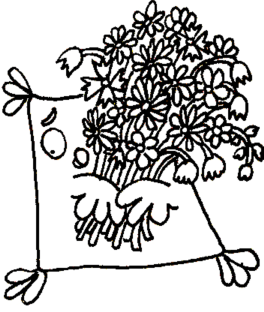
\includegraphics[scale=0.5]{15}}
\end{figure}
\end{SBSection*}

\end{song}

%\twocolumn
\begin{song}{Белая гвардия}{}{Белая гвардия}{Белая гвардия}{}{}

Проигрыш: (2 раза)\par 
\Ch{Am}{} \Ch{D}{} \Ch{G}{} \Ch{C}{} \Ch{Am}{} \Ch{H7}{} \Ch{Em}\\

\Ch{Em}{Белая} гвардия, белый снег,\par
\Ch{Am7}{Белая} музыка революций.\par
\Ch{D7}{Белая} женщина, нервный смех,\par
\Ch{G}{Белого} платья слегка коснуться.\par
 
Белой рукой распахнуть окно,\par
Белого света в нем не видя.\par
Белое выпить до дна вино,\par
В красную улицу в белом выйти.\\

Припев:\par
\ttКог\Ch{Em}{да} ты вернешься,\par
\ttВсе будет и\Ch{Am}{на}че, и нам бы узнать друг друга,\par
\ttКог\Ch{D7}{да} ты вернешься,\par
\ttА я не же\Ch{G}{на} и даже \Ch{H7}{не} подруга.\par
\ttКог\Ch{C}{да} ты вернешься,\par
\ttКо мне, так без\Ch{Am}{ум}но тебя любившей в прошлом,\par
\tt\Ch{D7}{Ко}гда ты вернешься -\par
\ttУвидишь, что ж\Ch{G}{ре}бий давно и не \Ch{E7}{нами} брошен.\\

Проигрыш.\\
 
\newpage
Сизые сумерки прошлых лет\par
Робко крадутся по переулкам.\par
В этом окне еле брезжит свет,\par
Ноты истрепаны, звуки гулки.\par
Тонкие пальцы срывают аккорд...\par
Нам не простят безрассудного дара.\par
Бьются в решетку стальных ворот\par
Пять океанов земного шара.\\

Припев. \par
Проигрыш.\\
 
Красный трамвай простучал в ночи,\par
Красный закат догорел в бокале,\par
Красные-красные кумачи\par
С красных деревьев на землю упали.\par
Я не ждала тебя в октябре,\par
Виделись сны, я листала сонник:\par
Красные лошади на заре\par
Били копытами о подоконник.\\

Припев:\par
\ttКогда ты вернешься,\par
\ttВсе будет иначе, и нам бы узнать друг друга,\par
\ttКогда ты вернешься,\par
\ttА я не жена и даже не подруга.\par
\ttКогда ты вернешься,\par
\ttВернешься в наш город обетованный,\par
\ttКогда ты вернешься -\par
\ttТакой невозможный и такой желанный?\\

Проигрыш.\par

\end{song}

%\twocolumn
\begin{song}{Перевал}{}{Песни у костра}{Песни у костра}{}{}


\Ch{Am}{Про}сто нечего нам \Ch{Dm}{боль}ше терять\par
\Ch{E}{Всё} нам вспомнится на \Ch{Am}{Страшном} суде.\par
Эта ночь легла, как \Ch{Dm}{тот} перевал,\par
\Ch{G}{За} которым испол\Ch{C}{нень}е надежд.\par
\Ch{A7}{Про}сто прожитое—про\Ch{Dm}{жи}то зря, \Ch{G}{}\par
Но не в этом, пони\Ch{C}{мае}шь ли, соль… \Ch{Am}{}\par
Слышишь, падают дож\Ch{Dm}{ди} октября.\par
\Ch{E}{Ви}дишь, старый дом сто\Ch{Am}{ит} средь лесов.\\

Мы затопим в доме печь, в доме печь,\par
Мы гитару позовем со стены.\par
Просто нечего нам больше беречь,\par
Ведь за нами все мосты сожжены.\par
Все мосты, все перекрёстки дорог,\par
Все прошёптанные тайны в ночи.\par
Каждый сделал все, что смог, все, что смог,\par
Мы об этом помолчим, помолчим.\\


И луна взойдет заплывшей свечой,\par
Ставни скрипнут  на ветру, на ветру.\par
Ах, как я тебя люблю горячо,\par
Это годы не сотрут, не сотрут.\par
Мы оставшихся друзей соберем,\par
Мы набьем картошкой старый рюкзак,\par
Люди спросят: "Что за шум, что за гам?"\par
Мы ответим: "Просто так,  просто так”...\\

\newpage

    Просто так идут дожди в октябре,\par
    И потеряны от счастья ключи.\par
    Это всё, конечно, мне, конечно, мне,\par
    Но об этом помолчим, помолчим.\par
    Просто прожитое—прожито зря,\par
    Но не в этом, понимаешь ли, соль…\par
    Слышишь, падают дожди октября.\par
    Видишь, старый дом стоит средь лесов.\par


\begin{SBSection*}
\begin{figure}[b!]
\center{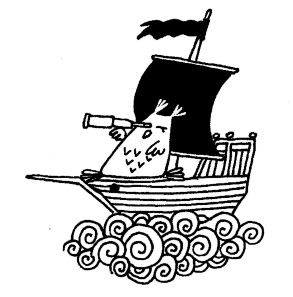
\includegraphics[scale=0.5]{22}}
\end{figure}
\end{SBSection*}

\end{song}

%\twocolumn
\begin{song}{Ленинградская (Все расстояния)}{}{Песни у костра}{Песни у костра}{}{}

\Ch{Am}{Все} расстоянья когда-нибудь в круг замы\Ch{E}{ка}ются,\par
\Ch{E}{Все} из разлук обязательно \Ch{E7}{встре}чей кон\Ch{Am}{ча}ются;\par
Должны про\Ch{Dm}{плыть} вокруг Зем\Ch{G}{ли,}\par
Вернуться в \Ch{C}{га}вань кораб\Ch{F}{ли,}\par   
Все поез\Ch{Dm}{да} в свои вер\Ch{E}{нуть}ся горо\Ch{Am}{да.}\\
 
Шумный вокзал то встречает друзей , то прощается,\par
Мы расстаемся, но снова назад возвращаемся -\par
Чтоб снова встать в огромный круг,\par
И снова знать, что рядом друг ,\par
И песни петь, чтоб больше не было разлук.\\
 
Все расстоянья когда-нибудь в круг замыкаются,\par
Все из разлук обязательно встречей кончаются;\par
И через год, и через пять,\par
Мы с вами встретимся опять,\par
Ничто не сможет нашей дружбе помешать.\par

\end{song}

%\twocolumn
\begin{song}{Десять капель}{}{Танцы Минус}{Танцы Минус}{}{}

Проигрыш: (2 раза)\par 
\Ch{C}{} \Ch{E}{} \Ch{Am}{} \Ch{F}{} \Ch{C}{} \Ch{E}{} \Ch{Am}{} \Ch{F}{}

\Ch{C}{Де}сять капель дож\Ch{E}{дя} у тебя на пле\Ch{Am}{че}\par
Ты забыла свой \Ch{F}{зонт,} ты спешила ко \Ch{C}{мне.}\par
Десять капель дож\Ch{E}{дя} на плече у те\Ch{Am}{бя,}\par
Десять капель люб\Ch{F}{ви,} десять капель ог\Ch{C}{ня}\\

Припев:\\(Три первых слова в припеве дублируются вторым голосом)\par
\tt\Ch{C}{Т}воя\Ch{E}{} ладо\Ch{Am}{нь} горит\Ch{F}{} в моих руках\par
\tt\Ch{C}{Л}юбви\Ch{E}{ }пож\Ch{Am}{ар} горит в тво\Ch{F}{их} глазах\\

Проигрыш.\\

Время делает шаг, время делает круг\par
Мы забудем друзей, мы забудем подруг\par
Просто выпьем вина из любви и огня\par
Десять капель меня, десять капель тебя\\

Припев.\\

Голос твой в тишине околдует меня\par
Ярким жарким огнем стану я до утра\par
Ты прикажешь гори, и я вспыхну любя\par
В этом пламени ты, в этом пламени я.\par

\end{song}

%\twocolumn
\begin{song}{Макет}{}{Песни у костра}{Сказка}{}{}
sadfsfthanks,\par
\begin{SBOpGroup}
asdas\
\end{SBOpGroup}
\begin{SBSection*}fdf\end{SBSection*}
\begin{SBVerse*}\end{SBVerse*}
\begin{SBChorus*}\end{SBChorus*}

\begin{SBOccurs}{23}
dsf
\end{SBOccurs}

\begin{SBSection*}
\begin{figure}[b!]
\center{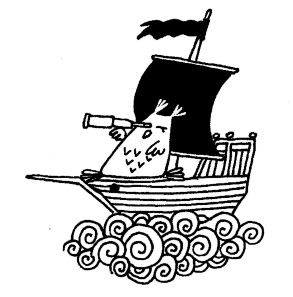
\includegraphics[scale=0.5]{22}}
\end{figure}
\end{SBSection*}
\end{song}

\mainmatter

\renewcommand{\footrulewidth}{0.0pt}
\renewcommand{\item}{\par\hangindent=40pt}
\renewcommand{\subitem}{\par\hangindent=40pt \hspace*{20pt}}
\renewcommand{\subsubitem}{\par\hangindent=40pt \hspace*{30pt}}

\newpage
\raggedright%\documentclass[a5paper,11pt]{book}
%\usepackage{fancyhdr}
%\usepackage[chordbk]{songbook}
%
%\usepackage[T2A]{fontenc}
%\usepackage[utf8]{inputenc}
%\usepackage[russian]{babel}
%
%\title{A Church Songbook}
%\author{}
%\date{Revised:  \RevDate}
%
%\newcommand{\RelDate}{13 November'19}
%\newcommand{\RevDate}{\today}

\documentclass[11pt,a5paper]{book}
\usepackage[a5paper]{geometry}
\usepackage[chordbk]{songbook}
\usepackage[T2A]{fontenc}
\usepackage[utf8]{inputenc}
\usepackage[russian]{babel}
\usepackage{cmap} % для работы поиска кириллицы в pdf

%\usepackage{amsmath,amsthm,amssymb}
%\usepackage{mathtext}


\usepackage[pdftex]{graphicx}
\usepackage{lscape}
%\usepackage{vmargin}
\usepackage{textcomp}
\usepackage{setspace}
%\usepackage{marvosym}
\usepackage{gensymb} %%%for \micro tag
\usepackage{upgreek} %%% \upmu
\usepackage{tipa}
\usepackage{phonetic}
%\usepackage[greek,english]{babel}
\usepackage{threeparttable}
\usepackage{multirow}
\usepackage{harvard}
\usepackage{longtable}
\renewcommand{\sectionmark}[1]{\markright{#1}}
\renewcommand{\chaptermark}[1]{\markboth{#1}{}}
\addto\captionsenglish{\renewcommand{\bibname}{References}}
\usepackage{latexsym,fancyhdr}

\newcommand{\RelDate}{26 Апреля'1984}
\newcommand{\RevDate}{\today}

%%%
% C.C.L.I. license number definition; for copyright licensing info.
% One of these macros will be manually inserted into the {CpyRt}
% parameter of the {song} environment.
%
%       \CCLInumber - The actual copyright license number.  Don't
%               insert this command in the {CpyRt} parameter, use one
%               of the others.
%       \CCLIed - Indicates a song falls under our CCLI license.
%       \NotCCLIed - Indicates a song doesn't fall under our CCLI
%               license.  Public Domain songs fall into this category.
%       \PGranted - We have received specific permission from the
%               copyright holder to use this song.
%       \PPending - We are in the process of obtaining permission to
%               use this song.
%%%
\newcommand{\CCLInumber}{Your CCLI Number}
\newcommand{\CCLIed}{{\CpyRtInfoFont (CCLI \CCLInumber)}}
\newcommand{\NotCCLIed}{\relax}
\newcommand{\PGranted}{\relax}
\newcommand{\PPending}{{\CpyRtInfoFont (Permission Pending)}}

%%%
% Title page information.
%%%
\title{ Сказочный песенник}
\author{}
\date{Созданно:  \RevDate}


%%%
% Define fonts to use in the headers and footers of the songbook.
%%%
\newcommand{\LHeadFont}{\normalsize}            % = cmr12  at 12pt
\newcommand{\CHeadFont}{\normalsize\rm}         % = cmr12  at 12pt
\newcommand{\RHeadFont}{\normalsize}            % = cmr12  at 12pt
\newcommand{\LFootFont}{\scriptsize}            % = cmr8   at  8pt
\newcommand{\CFootFont}{\tiny\myTinySF}         % = cmss8  at  8pt
\newcommand{\RFootFont}{\scriptsize}            % = cmr8   at  8pt

%%%
% Turn on and define fancy page heading/footing definition.
%%%
\pagestyle{fancy}

\ifChordBk
  % It's a words & chords songbook...
%  \addtolength{\headwidth}{\marginparsep}
%  \addtolength{\headwidth}{\marginparwidth}
  \renewcommand{\headrulewidth}{0.0pt}
  \renewcommand{\footrulewidth}{0.0pt}
%  \fancyhead[LE,RO]{\LHeadFont\emph{\leftmark\/}}
%  \fancyhead[CE,CO]{\CHeadFont\thepage}
  \fancyhead[RE,LO]{~}
\else\ifOverhead
  % It's an overhead...
  \renewcommand{\footrulewidth}{0pt}
  \renewcommand{\headrulewidth}{0pt}
  \fancyhead[LE,RO]{}
  \fancyhead[CE,CO]{}
  \fancyhead[RE,LO]{}
\else\ifWordBk
  % It's a words only songbook...
  \addtolength{\headwidth}{\marginparsep}
  \addtolength{\headwidth}{\marginparwidth}
  \renewcommand{\headrulewidth}{0.0pt}
  \renewcommand{\footrulewidth}{0.0pt}
  \fancyhead[LE,RO]{\LHeadFont A Church Songbook}
  \fancyhead[CE,CO]{\CHeadFont\thepage}
  \fancyhead[RE,LO]{\RHeadFont\RelDate}
\fi\fi\fi

%\fancyfoot[LE,RO]{\LFootFont Property of The Church}
%\ifSongEject
%  \fancyfoot[CE,CO]{\CFootFont \RevDate}
%\else
%  \fancyfoot[CE,CO]{\CFootFont}
%\fi
%\fancyfoot[RE,LO]{\RFootFont Material used by permission.}

%%%
% Turn on/off index-file generation.  Uncomment the \makeindex line to
% turn index generation on;  comment it out to turn index generation
% off.
%%%
\makeTitleIndex         %% Title and First Line Index.
\makeTitleContents      %% Table of Contents.
\makeKeyIndex           %% Index of song by key.
\graphicspath{{img/}} % папка с картинками
\DeclareGraphicsExtensions{.pdf,.png,.jpg} % форматы, которые будем считать картинками

%\newenvironment{song}[7][Y]{
%% Comment markers to negate
%\if#1Y\ExcludeSongfalse\else\ExcludeSongtrue\fi% the newline.
%\ifPrintAllSongs\ExcludeSongfalse\fi
%\SongMarkboth{\relax}{\relax}
%\SBinSongEnvtrue
%\renewcommand{\SBinSongEnv}{\True}
%\ifWordsOnly
%	\setlength{\parindent}{0pt}
%\fi

%%%
% Redefine fonts from SongBook style that I don't like.
%%%
\font\myTinySF=cmss8 at 8pt
\renewcommand{\CpyRtInfoFont}{\tiny\myTinySF}


%
%\font\myTinySF=cmss8    at  8pt
%\font\myHugeSF=cmssbx10 at 25pt
%\renewcommand{\CpyRtInfoFont}{\tiny\myTinySF}
%\newcommand{\myTitleFont}{\Huge\myHugeSF}
%\newcommand{\mySubTitleFont}{\large\sf}

%%% Работа с русским языком
%\usepackage[no-math]{fontspec}      %% подготавливает загрузку шрифтов Open Type, True Type и др.
%\defaultfontfeatures{Ligatures={TeX},Renderer=Basic}  %% свойства шрифтов по умолчанию
%\setmainfont[Ligatures={TeX,Historic}]{Times New Roman} %% задаёт основной шрифт документа
%\setsansfont{Helvetica Neue}                    %% задаёт шрифт без засечек

%\newfontfamily{\allods}{AllodsWest}

\newcommand{\SBPubDomm}{~}
\renewcommand{\CpyRt}[3][Y]{%
\if#1Y\begin{center}\fi
\if\blank{#2}%
\if\blank{#3}%
{\CpyRtFont\copyright \SBUnknownTag{} \CpyRtInfoFont}%
\else
{\CpyRtFont\copyright \SBUnknownTag{} \CpyRtInfoFont #3}%
\fi%
\else%
\ifthenelse{\equal{#2}{\SBPubDomm}}
{%then
{\CpyRtFont #2 \CpyRtInfoFont #3}%
}{%else
{\CpyRtFont #2 \CpyRtInfoFont #3}%
}%fi
\fi%
\if#1Y\end{center}\fi
}


\newcommand{\SBUnknownTagg}{~}
\renewcommand{\WAndM}[2][Y]{~}
\renewcommand{\WAndM}[2][Y]{%
\if#1Y\begin{center}\fi
\if\blank{#2}%
{\SBUnknownTagg}%
\else
{~}%
\fi
\if#1Y\end{center}\fi
}

\renewcommand{\STitle}[3][Y]{%
\setcounter{SBVerseCnt}{0}%
\setcounter{SBSectionCnt}{0}%
\ifExcludeSong\relax%
	\else\keyIndex{{\protect\sbChord#3\protect\relax} -- #2}{\theSBSongCnt}\fi%
	\vspace{\SpaceAboveSTitle}%
\if#1Y\begin{center}\fi
	{}{\STitleFont\LARGE #2}%
	\ifWordsOnly\relax\else\fi%
	\if#1Y\end{center}\fi
\STitleMarkboth{#2}{\relax}%
}


%\renewenvironment{SBOpGroup}{%
%	\sbSetsbBaselineSkipAmt%
%	\bgroup%
%	\begin{list}{\hbox{}}
%	  {\setlength {\leftmargin}
%		{\HangAmt}
%		\setlength{\itemindent}
%			{-\HangAmt}
%		\setlength{\listparindent}{-\HangAmt}
%		\setlength{\topsep}{0pt}
%		\setlength{\parsep}{0pt}
%		\setlength{\labelwidth}{0pt}
%		\setlength{\labelsep}{0pt}
%		\setlength{\baselineskip} {\sbBaselineSkipAmt}
%	}%\item}
%{\end{list}%
\newcommand{\SBChorusTagg}{Припев}
\renewenvironment{SBChorus}{%
\sbSetsbBaselineSkipAmt%
\bgroup%
\SBChorusMarkright{\SBChorusTag}
\begin{list}{{\SBChorusTagFont\SBChorusTagg}}
{\setlength {\leftmargin}
{\LeftMarginSBChorus + \HangAmt}
\setlength{\itemindent}
{-\HangAmt}
\setlength{\listparindent}{-\HangAmt}
\setlength{\parsep}
{0pt}
\setlength{\baselineskip} {\sbBaselineSkipAmt}
}%
\item}
{\end{list}%
\egroup%
\SpaceAfterChorus%
}

\renewcommand{\tt}{\indent \indent}
%\renewcommand{\nt}{\noindent}


\usepackage{amsmath}

\makeArtistIndex
\makeTitleIndex         %% Title and First Line Index.
\makeTitleContents      %% Table of Contents.
\makeKeyIndex           %% Index of song by key.
%\usepackage{printallsongs}

\begin{document} 
\maketitle

\mainmatter


\begin{song}{Вожатский гимн}{}{Сказка}{Сказка}{}{}

По \Ch{Am}{ла}герю подъём, нас горн зовёт!\par
Забудь о том, что ночь была бес\Ch{C}{сон}ною\par
Смо\Ch{Dm}{чи} водою \Ch{G}{ве}ки воспа\Ch{C}{лён}\Ch{F}{ные}\par    
По\Ch{Dm}{вя}зывай свой \Ch{E}{галс}тук — и впе\Ch{Am (A7)}{рёд!}\par
Смо\Ch{Dm}{чи} водою \Ch{G}{ве}ки воспа\Ch{C}{лён}\Ch{F}{ные}\par    
По\Ch{Dm}{вя}зывай свой \Ch{E}{галс}тук — и впе\Ch{Am (A7)}{рёд!}\par

%	\begin{SBChorus*}
\ttНе\Ch{E}{про}сто воспитывать \Ch{Am}{но}вых людей,\par
\ttНу \Ch{E}{что} ж, это наша с то\Ch{Am}{бою} свя\Ch{A7}{ты}ня.\par
\ttМой \Ch{Dm}{друг}, нам до\Ch{G}{ве}рили \Ch{C}{ду}ши де\Ch{F}{тей},\par
\ttИх \Ch{Dm}{ра}достный \Ch{Am}{смех} нам на\Ch{E}{гра}да от\Ch{Am}{ны}не.\par
\ttМой \Ch{Dm}{друг}, нам до\Ch{G}{ве}рили \Ch{C}{ду}ши де\Ch{F}{тей},\par
\ttИх \Ch{Dm}{ра}достный \Ch{Am}{смех} нам на\Ch{E}{гра}да от\Ch{Am}{ны}не.\\
%\end{SBChorus*}

Отбой, засыпает детвора.\par
Взгляни на их улыбки полусонные,\par
Пускай им снятся острова зелёные,\par
А нам опять работать до утра!\par
Пускай им снятся острова зелёные,\par
А нам опять работать до утра!\par

\tt И пусть от бессилья затихнешь не раз,\par
\ttИ голос усталый до хрипа натружен,\par
\ttПусть будут умней и счастливее нас\par
\ttТе дети, в которых вложили мы души!\par
\ttПусть будут умней и счастливее нас\par
\ttТе дети, в которых вложили мы души!

\end{song}

\begin{song}{Сказка в неглиже}{}{Сказка}{Сказка}{}{}

Есть у \Ch{C}{каж}дого добрая сказка в ду\Ch{F}{ше,}\par 
Надо \Ch{G}{толь}ко прочесть этой сказки стра\Ch{C}{ни}цы.\par
В тиши\Ch{C}{не}, разо\Ch{C7}{де}тая вся в негли\Ch{F}{же,}\par
Пусть на\Ch{G}{ве}ки она, пусть на\Ch{F}{ве}ки она сохра\Ch{C}{ни}тся. \Ch{C7}{ }\par 
В тиши\Ch{F}{не,} разо\Ch{G}{де}тая вся в негли\Ch{C}{же,} \Ch{Am}{}\par
Пусть на\Ch{F}{ве}ки она, пусть на\Ch{G}{ве}ки она сохра\Ch{C}{ни}тся.\\


\ttЭту сказку пред другом раскрыть поспеши,\par
\ttА врагу не спеши эту сказку поведать.\par
\ttПусть растут и читают ее малыши.\par
\ttБудь добрей, и тебя минут всякие беды.\par
\ttПусть растут и читают ее малыши.\par
\ttБудь добрей, и тебя минут всякие беды.\\


\Ch{C7}{}Будет \Ch{F}{мно}го распутий, \Ch{G}{до}рог и тре\Ch{C}{вог.}\Ch{Am}{}\par
На вис\Ch{F}{ки} твои ляжет \Ch{G}{не}тающий \Ch{C}{ин}ей, \Ch{C7}{}\par
И пой\Ch{F}{мёшь,} научившись чи\Ch{G}{тать} между \Ch{C}{строк:} \Ch{Am}{}\par
Даже \Ch{F}{гнус}ный злодей \Ch{G}{в} этой сказке не\Ch{C}{ви}нен. \Ch{C7}{}\par
И пой\Ch{F}{мёшь,} научившись чи\Ch{G}{тать} между ст\Ch{C}{рок:} \Ch{A}{}\par
Даже \Ch{F}{гнус}ный злодей \Ch{G}{в} этой сказке не\Ch{C}{ви}нен.\\

\Ch{C}{} \Ch{G}{} \Ch{F}{} \Ch{G}{} \Ch{C}{} \Ch{C7}{}\par
\Ch{C}{} \Ch{G}{} \Ch{F}{} \Ch{G}{} \Ch{C}{}
\end{song}

%\twocolumn
\begin{song}{Вожатский марш}{}{Сказка}{Сказка}{}{}

Есть на\Ch{Am}{род} у нас весёлый,\par
Самой \Ch{C}{луч}шей в мире пробы,\par
Песни \Ch{G}{петь} всегда мас\Ch{C}{так.}\Ch{A7}{}\par
Он всег\Ch{Dm}{да} всего добьётся,\par
Он Вожа\Ch{Am}{ты}ми зовётся,\par
\Ch{E}{Так} и только \Ch{Am (A7)}{так!}\par
Он всег\Ch{Dm}{да} всего добьётся,\par
Он Во\Ch{Am}{жа}тыми зовётся,\par
\Ch{E}{Так} и только \Ch{Am (A7)}{так!}\\

Домосед привязан к дому\par
И по случаю такому,\par
Он из дома — ни на шаг!\par
А вожатый — он в дороге,\par
Он готов в огонь и в воду,\par
Так и только так!\par
А вожатый — он в дороге,\par
Он готов в огонь и в воду,\par
Так и только так!\\
\newpage
Жадный денежки считает,\par
Все считает и считает,\par
К пятаку кладет пятак.\par
А вожатый деньги тратит,\par
Не боясь, что их не хватит,\par
Так и только так!\par
А вожатый деньги тратит,\par
Не боясь, что их не хватит,\par
Так и только так!\\

Холостяк в любовь не верит,\par
Все не верит и не верит,\par
Потому что холостяк.\par
А вожатых не влюблённых\par
Не найдёшь определённо,\par
Так и только так!\par
А вожатых не влюблённых\par
Не найдёшь определённо,\par
Так и только так!\par

\begin{SBSection*}
\begin{figure}[b!]
\center{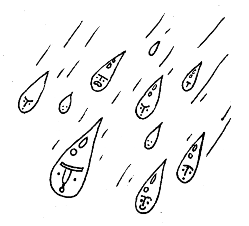
\includegraphics[scale=0.5]{16}}
\end{figure}
\end{SBSection*}
\end{song}

%\twocolumn
\begin{song}{Двадцать дней}{}{Сказка}{Сказка}{}{}


Двадцать дн\Ch{Dm}{ей} – это смена без дня.\par
“Маловато”,– вам скажут друзь\Ch{Gm}{я,}\par
А вожатый отв\Ch{C}{ет}ит люб\Ch{F}{ой}:\par
Это ср\Ch{Gm}{ок} очень д\Ch{A}{аж}е больш\Ch{Dm}{ой!}\\
 

Припев:\par
\ttМожно з\Ch{Gm C}{а-а-а-а} него усп\Ch{Dm}{ет}ь,\par
\ttНаприм\Ch{Gm}{ер,} полмилли\Ch{A}{он}а песен сп\Ch{Dm}{еть,}\par
\ttНо не к\Ch{Gm}{ажд}ый ведь поймет,\par
\ttКак так быстро раскрыв\Ch{A}{ат}ься может р\Ch{Dm}{от!}\\


Для полярника это не срок:\par
Не успеет просохнуть носок.\par
А вожатый успеет подряд \par
Вымыть, высушить сотню ребят!\\

Припев:\par
\ttВедь за смену, как за год \par
\ttСтолько разных мелочей произойдет,\par
\ttНо пока что нам везет,\par
\ttНас начальство для чего-то бережёт.\\


\newpage
Хоть и длинными кажутся дни,\par
Но как миг пролетели они.\par
Будешь долго потом вспоминать,\par
Как в отбой ты любил слово «СПАААТЬ!!!»\\

Припев:\par
\tt          	— Говорят за двадцать дней \par
\tt          	Все узнаешь о напарнице своей…\par
\tt          	— Только это ерунда,\par
\tt          	Обо всем ты не узнаешь никогда!\\

Смена вряд ли даст ответ:\par
Ты нашел свое призванье или нет.\par
Так что надо продолжать,\par
Двадцать раз по двадцать суток отсчитать!\\

\begin{SBSection*}
\begin{figure}[b!]
\center{\includegraphics[scale=0.5]{17}}
\end{figure}
\end{SBSection*}

\end{song}

%\twocolumn
\begin{song}{Непогода}{}{Павел Смеян}{Павел Смеян}{}{}

\Ch{D}{Из}менения в природе \Ch{G}{пр}оисходят г\Ch{A}{од} от года,\par
\Ch{D}{Не}погода нынче в моде,\Ch{G}{} н\Ch{F#7}{епог}ода, непогода,\par
\Ch{}Hm{Слов}но из вод\Ch{F#7}{опро}вода \Ch{D7}{ль}ёт на нас с неб\Ch{G}{ес} во\Ch{Hm}{да…}\par
Полг\Ch{G}{од}а плох\Ch{A}{ая} пог\Ch{D}{од}а, \Ch{Hm}{пол}го\Ch{G}{да} — совс\Ch{A}{ем} нику\Ch{D}{да}.\par
Полг\Ch{G}{од}а плох\Ch{A}{ая} пог\Ch{D}{од}а, \Ch{Hm}{пол}го\Ch{G}{да} — сов\Ch{F#7}{сем} нику\Ch{Hm}{да.}\\


\SBChorusTagg:\par
\ttНикуда, нику\Ch{Em}{да н}ельз\Ch{A}{я} укр\Ch{D}{ы}ться н\Ch{Hm}{ам,}\par
\ttНо откладывать ж\Ch{Em}{изнь} ни\Ch{A}{как} нель\Ch{D}{зя}, \Ch{Hm}{}\par
\ttНикуда, нику\Ch{Em}{да, н}о зн\Ch{A}{ай}, что гд\Ch{D}{е}-то т\Ch{Hm}{ам}\par
\ttКто-то ищет теб\Ch{G}{я} сре\Ch{F#7}{ди д}ожд\Ch{Hm}{я.} \Ch{A}{}\\


Грома грозные раскаты от заката до восхода,\par
За грехи людские плата — непогода, непогода,\par
Не ангина, не простуда, посерьёзнее беда.\par
Полгода плохая погода, полгода — совсем никуда\par,
Полгода плохая погода, полгода — совсем никуда.\\\


\SBChorusTagg:\par
\ttНикуда, нику\Ch{Em}{да н}ельз\Ch{A}{я} укр\Ch{D}{ы}ться н\Ch{Hm}{ам,}\par
\ttНо откладывать ж\Ch{Em}{изнь} ни\Ch{A}{как} нель\Ch{D}{зя}, \Ch{Hm}{}\par
\ttНикуда, нику\Ch{Em}{да, н}о зн\Ch{A}{ай}, что гд\Ch{D}{е}-то т\Ch{Hm}{ам}\par
\ttКто-то ищет теб\Ch{G}{я} сре\Ch{F#7}{ди д}ожд\Ch{Hm}{я.} \Ch{A}{}\\


\end{song}

%\twocolumn
\begin{song}{Птенцы}{}{Сказка}{Сказка}{}{}

\Ch{Am}{}  \Ch{Am}{}

Как птенцы из гнез\Ch{Dm}{да} мы \Ch{E}{вы}па\Ch{Am}{ли.}\par
Ты не бойся при\Ch{Dm}{хо}да \Ch{G}{ве}че\Ch{C}{ра.}\par
Под та\Ch{A7}{ки}ми боль\Ch{F}{ши}ми \Ch{A7}{ли}па\Ch{Dm}{ми}\par
Нам с то\Ch{F}{бой} опа\Ch{Dm}{сать}ся \Ch{F}{не}\Ch{E}{че}\Ch{Am}{го.}\\
 
Под такими густыми звёздами -\par
Разве их не для нас рассыпали,\par
Мы не против гнездовья - просто мы\par
Из него ненароком выпали.\\

Это только вначале кажется,\par
Что без дома прожить нельзя никак,\par
Что важней пропитанья кашица,\par
Чем огромные звёзды на небе.\\

Ты не бойся ни тьмы, ни холода.\par
Будет день и найдётся пища нам,\par
Мы ещё пролетим над городом\par
На крыле до небес возвышенном.\\

Пролетим ещё - эка невидаль\par
Над Нью-Йорком, Парижем, Триполи\par
И над липой, откуда некогда,\par
Как птенцы из гнезда мы выпали.\\

Как птенцы из гнезда мы выпали.\par
Ты не бойся прихода вечера.\par
Под такими большими липами\par
Нам с тобой опасаться нечего.\\

\end{song}

%\twocolumn
\begin{song}{Продавец зонтиков}{}{Веня Дркин}{Веня Дркин}{}{}

\Ch{Am}{Город} этот выдумал о\Ch{Dm}{дин} художник,\par
\Ch{G}{Лю}ди в нем не знали, что та\Ch{C}{ко}е дождик.\par
\Ch{A7}{Про}сто не слыхали, что та\Ch{Dm}{ко}е зонтик –\par
\Ch{E7}{Вот} такие люди жили в \Ch{Am}{го}роде том.\par
И один чудак, в старый плащ одетый,\par
Продавал там зонтики зимой и летом,\par
Продавал там зонтики зимой и летом\par
И такую песенку он напевал:\\

\SBChorusTagg:\par
\tt“Господа, купите зонтик.\par
\ttБелый зонтик, красный зонтик,\par
\ttЖелтый зонтик, синий зонтик –\par
\ttМожет пригодится вам.”\\

Были домики у них из пластилина,\par
Из пустых коробочек автомашины,\par
И, не опасаясь никакой ангины,\par
Маленькие люди жили в городе том.\par
Маленькие были у людей заботы:\par
Шли они в кино или в театр с работы.\par
Вечером в подъезде целовался кто-то.\par
Все шутили и смеялись над стариком.\\


\SBChorusTagg.\\

\newpage

Маленькое небо как-то вдруг намокло,\par
В крошечных домишках задрожали стекла,\par
И огромный дождь пошел гулять по крышам,\par
Сразу все схватили насморк в городе том.\par
Вспомнили тут люди о торговце старом,\par
Кинулись искать его по всем базарам,\par
Но исчез торговец со своим товаром.\par
Только песенка осталась в память о нем:\\

\SBChorusTagg.\par

\begin{SBSection*}
\begin{figure}[b!]
\center{\includegraphics[scale=0.5]{15}}
\end{figure}
\end{SBSection*}

\end{song}

%\twocolumn
\begin{song}{Белая гвардия}{}{Белая гвардия}{Белая гвардия}{}{}

Проигрыш: (2 раза)\par 
\Ch{Am}{} \Ch{D}{} \Ch{G}{} \Ch{C}{} \Ch{Am}{} \Ch{H7}{} \Ch{Em}\\

\Ch{Em}{Белая} гвардия, белый снег,\par
\Ch{Am7}{Белая} музыка революций.\par
\Ch{D7}{Белая} женщина, нервный смех,\par
\Ch{G}{Белого} платья слегка коснуться.\par
 
Белой рукой распахнуть окно,\par
Белого света в нем не видя.\par
Белое выпить до дна вино,\par
В красную улицу в белом выйти.\\

Припев:\par
\ttКог\Ch{Em}{да} ты вернешься,\par
\ttВсе будет и\Ch{Am}{на}че, и нам бы узнать друг друга,\par
\ttКог\Ch{D7}{да} ты вернешься,\par
\ttА я не же\Ch{G}{на} и даже \Ch{H7}{не} подруга.\par
\ttКог\Ch{C}{да} ты вернешься,\par
\ttКо мне, так без\Ch{Am}{ум}но тебя любившей в прошлом,\par
\tt\Ch{D7}{Ко}гда ты вернешься -\par
\ttУвидишь, что ж\Ch{G}{ре}бий давно и не \Ch{E7}{нами} брошен.\\

Проигрыш.\\
 
\newpage
Сизые сумерки прошлых лет\par
Робко крадутся по переулкам.\par
В этом окне еле брезжит свет,\par
Ноты истрепаны, звуки гулки.\par
Тонкие пальцы срывают аккорд...\par
Нам не простят безрассудного дара.\par
Бьются в решетку стальных ворот\par
Пять океанов земного шара.\\

Припев. \par
Проигрыш.\\
 
Красный трамвай простучал в ночи,\par
Красный закат догорел в бокале,\par
Красные-красные кумачи\par
С красных деревьев на землю упали.\par
Я не ждала тебя в октябре,\par
Виделись сны, я листала сонник:\par
Красные лошади на заре\par
Били копытами о подоконник.\\

Припев:\par
\ttКогда ты вернешься,\par
\ttВсе будет иначе, и нам бы узнать друг друга,\par
\ttКогда ты вернешься,\par
\ttА я не жена и даже не подруга.\par
\ttКогда ты вернешься,\par
\ttВернешься в наш город обетованный,\par
\ttКогда ты вернешься -\par
\ttТакой невозможный и такой желанный?\\

Проигрыш.\par

\end{song}

%\twocolumn
\begin{song}{Перевал}{}{Песни у костра}{Песни у костра}{}{}


\Ch{Am}{Про}сто нечего нам \Ch{Dm}{боль}ше терять\par
\Ch{E}{Всё} нам вспомнится на \Ch{Am}{Страшном} суде.\par
Эта ночь легла, как \Ch{Dm}{тот} перевал,\par
\Ch{G}{За} которым испол\Ch{C}{нень}е надежд.\par
\Ch{A7}{Про}сто прожитое—про\Ch{Dm}{жи}то зря, \Ch{G}{}\par
Но не в этом, пони\Ch{C}{мае}шь ли, соль… \Ch{Am}{}\par
Слышишь, падают дож\Ch{Dm}{ди} октября.\par
\Ch{E}{Ви}дишь, старый дом сто\Ch{Am}{ит} средь лесов.\\

Мы затопим в доме печь, в доме печь,\par
Мы гитару позовем со стены.\par
Просто нечего нам больше беречь,\par
Ведь за нами все мосты сожжены.\par
Все мосты, все перекрёстки дорог,\par
Все прошёптанные тайны в ночи.\par
Каждый сделал все, что смог, все, что смог,\par
Мы об этом помолчим, помолчим.\\


И луна взойдет заплывшей свечой,\par
Ставни скрипнут  на ветру, на ветру.\par
Ах, как я тебя люблю горячо,\par
Это годы не сотрут, не сотрут.\par
Мы оставшихся друзей соберем,\par
Мы набьем картошкой старый рюкзак,\par
Люди спросят: "Что за шум, что за гам?"\par
Мы ответим: "Просто так,  просто так”...\\

\newpage

    Просто так идут дожди в октябре,\par
    И потеряны от счастья ключи.\par
    Это всё, конечно, мне, конечно, мне,\par
    Но об этом помолчим, помолчим.\par
    Просто прожитое—прожито зря,\par
    Но не в этом, понимаешь ли, соль…\par
    Слышишь, падают дожди октября.\par
    Видишь, старый дом стоит средь лесов.\par


\begin{SBSection*}
\begin{figure}[b!]
\center{\includegraphics[scale=0.5]{22}}
\end{figure}
\end{SBSection*}

\end{song}

%\twocolumn
\begin{song}{Ленинградская (Все расстояния)}{}{Песни у костра}{Песни у костра}{}{}

\Ch{Am}{Все} расстоянья когда-нибудь в круг замы\Ch{E}{ка}ются,\par
\Ch{E}{Все} из разлук обязательно \Ch{E7}{встре}чей кон\Ch{Am}{ча}ются;\par
Должны про\Ch{Dm}{плыть} вокруг Зем\Ch{G}{ли,}\par
Вернуться в \Ch{C}{га}вань кораб\Ch{F}{ли,}\par   
Все поез\Ch{Dm}{да} в свои вер\Ch{E}{нуть}ся горо\Ch{Am}{да.}\\
 
Шумный вокзал то встречает друзей , то прощается,\par
Мы расстаемся, но снова назад возвращаемся -\par
Чтоб снова встать в огромный круг,\par
И снова знать, что рядом друг ,\par
И песни петь, чтоб больше не было разлук.\\
 
Все расстоянья когда-нибудь в круг замыкаются,\par
Все из разлук обязательно встречей кончаются;\par
И через год, и через пять,\par
Мы с вами встретимся опять,\par
Ничто не сможет нашей дружбе помешать.\par

\end{song}

%\twocolumn
\begin{song}{Десять капель}{}{Танцы Минус}{Танцы Минус}{}{}

Проигрыш: (2 раза)\par 
\Ch{C}{} \Ch{E}{} \Ch{Am}{} \Ch{F}{} \Ch{C}{} \Ch{E}{} \Ch{Am}{} \Ch{F}{}

\Ch{C}{Де}сять капель дож\Ch{E}{дя} у тебя на пле\Ch{Am}{че}\par
Ты забыла свой \Ch{F}{зонт,} ты спешила ко \Ch{C}{мне.}\par
Десять капель дож\Ch{E}{дя} на плече у те\Ch{Am}{бя,}\par
Десять капель люб\Ch{F}{ви,} десять капель ог\Ch{C}{ня}\\

Припев:\\(Три первых слова в припеве дублируются вторым голосом)\par
\tt\Ch{C}{Т}воя\Ch{E}{} ладо\Ch{Am}{нь} горит\Ch{F}{} в моих руках\par
\tt\Ch{C}{Л}юбви\Ch{E}{ }пож\Ch{Am}{ар} горит в тво\Ch{F}{их} глазах\\

Проигрыш.\\

Время делает шаг, время делает круг\par
Мы забудем друзей, мы забудем подруг\par
Просто выпьем вина из любви и огня\par
Десять капель меня, десять капель тебя\\

Припев.\\

Голос твой в тишине околдует меня\par
Ярким жарким огнем стану я до утра\par
Ты прикажешь гори, и я вспыхну любя\par
В этом пламени ты, в этом пламени я.\par

\end{song}

%\twocolumn
\begin{song}{Макет}{}{Песни у костра}{Сказка}{}{}
sadfsfthanks,\par
\begin{SBOpGroup}
asdas\
\end{SBOpGroup}
\begin{SBSection*}fdf\end{SBSection*}
\begin{SBVerse*}\end{SBVerse*}
\begin{SBChorus*}\end{SBChorus*}

\begin{SBOccurs}{23}
dsf
\end{SBOccurs}

\begin{SBSection*}
\begin{figure}[b!]
\center{\includegraphics[scale=0.5]{22}}
\end{figure}
\end{SBSection*}
\end{song}

\mainmatter

\renewcommand{\footrulewidth}{0.0pt}
\renewcommand{\item}{\par\hangindent=40pt}
\renewcommand{\subitem}{\par\hangindent=40pt \hspace*{20pt}}
\renewcommand{\subsubitem}{\par\hangindent=40pt \hspace*{30pt}}

\newpage
\raggedright\input{/home/p_a/git/ska3ka/ps.adx}

\centering\includegraphics[scale=0.5]{10}

\newpage
\raggedright\input{/home/p_a/git/ska3ka/ps.tdx}

\centering\includegraphics[scale=0.5]{11}

\end{document}


\centering\includegraphics[scale=0.5]{10}

\newpage
\raggedright%\documentclass[a5paper,11pt]{book}
%\usepackage{fancyhdr}
%\usepackage[chordbk]{songbook}
%
%\usepackage[T2A]{fontenc}
%\usepackage[utf8]{inputenc}
%\usepackage[russian]{babel}
%
%\title{A Church Songbook}
%\author{}
%\date{Revised:  \RevDate}
%
%\newcommand{\RelDate}{13 November'19}
%\newcommand{\RevDate}{\today}

\documentclass[11pt,a5paper]{book}
\usepackage[a5paper]{geometry}
\usepackage[chordbk]{songbook}
\usepackage[T2A]{fontenc}
\usepackage[utf8]{inputenc}
\usepackage[russian]{babel}
\usepackage{cmap} % для работы поиска кириллицы в pdf

%\usepackage{amsmath,amsthm,amssymb}
%\usepackage{mathtext}


\usepackage[pdftex]{graphicx}
\usepackage{lscape}
%\usepackage{vmargin}
\usepackage{textcomp}
\usepackage{setspace}
%\usepackage{marvosym}
\usepackage{gensymb} %%%for \micro tag
\usepackage{upgreek} %%% \upmu
\usepackage{tipa}
\usepackage{phonetic}
%\usepackage[greek,english]{babel}
\usepackage{threeparttable}
\usepackage{multirow}
\usepackage{harvard}
\usepackage{longtable}
\renewcommand{\sectionmark}[1]{\markright{#1}}
\renewcommand{\chaptermark}[1]{\markboth{#1}{}}
\addto\captionsenglish{\renewcommand{\bibname}{References}}
\usepackage{latexsym,fancyhdr}

\newcommand{\RelDate}{26 Апреля'1984}
\newcommand{\RevDate}{\today}

%%%
% C.C.L.I. license number definition; for copyright licensing info.
% One of these macros will be manually inserted into the {CpyRt}
% parameter of the {song} environment.
%
%       \CCLInumber - The actual copyright license number.  Don't
%               insert this command in the {CpyRt} parameter, use one
%               of the others.
%       \CCLIed - Indicates a song falls under our CCLI license.
%       \NotCCLIed - Indicates a song doesn't fall under our CCLI
%               license.  Public Domain songs fall into this category.
%       \PGranted - We have received specific permission from the
%               copyright holder to use this song.
%       \PPending - We are in the process of obtaining permission to
%               use this song.
%%%
\newcommand{\CCLInumber}{Your CCLI Number}
\newcommand{\CCLIed}{{\CpyRtInfoFont (CCLI \CCLInumber)}}
\newcommand{\NotCCLIed}{\relax}
\newcommand{\PGranted}{\relax}
\newcommand{\PPending}{{\CpyRtInfoFont (Permission Pending)}}

%%%
% Title page information.
%%%
\title{ Сказочный песенник}
\author{}
\date{Созданно:  \RevDate}


%%%
% Define fonts to use in the headers and footers of the songbook.
%%%
\newcommand{\LHeadFont}{\normalsize}            % = cmr12  at 12pt
\newcommand{\CHeadFont}{\normalsize\rm}         % = cmr12  at 12pt
\newcommand{\RHeadFont}{\normalsize}            % = cmr12  at 12pt
\newcommand{\LFootFont}{\scriptsize}            % = cmr8   at  8pt
\newcommand{\CFootFont}{\tiny\myTinySF}         % = cmss8  at  8pt
\newcommand{\RFootFont}{\scriptsize}            % = cmr8   at  8pt

%%%
% Turn on and define fancy page heading/footing definition.
%%%
\pagestyle{fancy}

\ifChordBk
  % It's a words & chords songbook...
%  \addtolength{\headwidth}{\marginparsep}
%  \addtolength{\headwidth}{\marginparwidth}
  \renewcommand{\headrulewidth}{0.0pt}
  \renewcommand{\footrulewidth}{0.0pt}
%  \fancyhead[LE,RO]{\LHeadFont\emph{\leftmark\/}}
%  \fancyhead[CE,CO]{\CHeadFont\thepage}
  \fancyhead[RE,LO]{~}
\else\ifOverhead
  % It's an overhead...
  \renewcommand{\footrulewidth}{0pt}
  \renewcommand{\headrulewidth}{0pt}
  \fancyhead[LE,RO]{}
  \fancyhead[CE,CO]{}
  \fancyhead[RE,LO]{}
\else\ifWordBk
  % It's a words only songbook...
  \addtolength{\headwidth}{\marginparsep}
  \addtolength{\headwidth}{\marginparwidth}
  \renewcommand{\headrulewidth}{0.0pt}
  \renewcommand{\footrulewidth}{0.0pt}
  \fancyhead[LE,RO]{\LHeadFont A Church Songbook}
  \fancyhead[CE,CO]{\CHeadFont\thepage}
  \fancyhead[RE,LO]{\RHeadFont\RelDate}
\fi\fi\fi

%\fancyfoot[LE,RO]{\LFootFont Property of The Church}
%\ifSongEject
%  \fancyfoot[CE,CO]{\CFootFont \RevDate}
%\else
%  \fancyfoot[CE,CO]{\CFootFont}
%\fi
%\fancyfoot[RE,LO]{\RFootFont Material used by permission.}

%%%
% Turn on/off index-file generation.  Uncomment the \makeindex line to
% turn index generation on;  comment it out to turn index generation
% off.
%%%
\makeTitleIndex         %% Title and First Line Index.
\makeTitleContents      %% Table of Contents.
\makeKeyIndex           %% Index of song by key.
\graphicspath{{img/}} % папка с картинками
\DeclareGraphicsExtensions{.pdf,.png,.jpg} % форматы, которые будем считать картинками

%\newenvironment{song}[7][Y]{
%% Comment markers to negate
%\if#1Y\ExcludeSongfalse\else\ExcludeSongtrue\fi% the newline.
%\ifPrintAllSongs\ExcludeSongfalse\fi
%\SongMarkboth{\relax}{\relax}
%\SBinSongEnvtrue
%\renewcommand{\SBinSongEnv}{\True}
%\ifWordsOnly
%	\setlength{\parindent}{0pt}
%\fi

%%%
% Redefine fonts from SongBook style that I don't like.
%%%
\font\myTinySF=cmss8 at 8pt
\renewcommand{\CpyRtInfoFont}{\tiny\myTinySF}


%
%\font\myTinySF=cmss8    at  8pt
%\font\myHugeSF=cmssbx10 at 25pt
%\renewcommand{\CpyRtInfoFont}{\tiny\myTinySF}
%\newcommand{\myTitleFont}{\Huge\myHugeSF}
%\newcommand{\mySubTitleFont}{\large\sf}

%%% Работа с русским языком
%\usepackage[no-math]{fontspec}      %% подготавливает загрузку шрифтов Open Type, True Type и др.
%\defaultfontfeatures{Ligatures={TeX},Renderer=Basic}  %% свойства шрифтов по умолчанию
%\setmainfont[Ligatures={TeX,Historic}]{Times New Roman} %% задаёт основной шрифт документа
%\setsansfont{Helvetica Neue}                    %% задаёт шрифт без засечек

%\newfontfamily{\allods}{AllodsWest}

\newcommand{\SBPubDomm}{~}
\renewcommand{\CpyRt}[3][Y]{%
\if#1Y\begin{center}\fi
\if\blank{#2}%
\if\blank{#3}%
{\CpyRtFont\copyright \SBUnknownTag{} \CpyRtInfoFont}%
\else
{\CpyRtFont\copyright \SBUnknownTag{} \CpyRtInfoFont #3}%
\fi%
\else%
\ifthenelse{\equal{#2}{\SBPubDomm}}
{%then
{\CpyRtFont #2 \CpyRtInfoFont #3}%
}{%else
{\CpyRtFont #2 \CpyRtInfoFont #3}%
}%fi
\fi%
\if#1Y\end{center}\fi
}


\newcommand{\SBUnknownTagg}{~}
\renewcommand{\WAndM}[2][Y]{~}
\renewcommand{\WAndM}[2][Y]{%
\if#1Y\begin{center}\fi
\if\blank{#2}%
{\SBUnknownTagg}%
\else
{~}%
\fi
\if#1Y\end{center}\fi
}

\renewcommand{\STitle}[3][Y]{%
\setcounter{SBVerseCnt}{0}%
\setcounter{SBSectionCnt}{0}%
\ifExcludeSong\relax%
	\else\keyIndex{{\protect\sbChord#3\protect\relax} -- #2}{\theSBSongCnt}\fi%
	\vspace{\SpaceAboveSTitle}%
\if#1Y\begin{center}\fi
	{}{\STitleFont\LARGE #2}%
	\ifWordsOnly\relax\else\fi%
	\if#1Y\end{center}\fi
\STitleMarkboth{#2}{\relax}%
}


%\renewenvironment{SBOpGroup}{%
%	\sbSetsbBaselineSkipAmt%
%	\bgroup%
%	\begin{list}{\hbox{}}
%	  {\setlength {\leftmargin}
%		{\HangAmt}
%		\setlength{\itemindent}
%			{-\HangAmt}
%		\setlength{\listparindent}{-\HangAmt}
%		\setlength{\topsep}{0pt}
%		\setlength{\parsep}{0pt}
%		\setlength{\labelwidth}{0pt}
%		\setlength{\labelsep}{0pt}
%		\setlength{\baselineskip} {\sbBaselineSkipAmt}
%	}%\item}
%{\end{list}%
\newcommand{\SBChorusTagg}{Припев}
\renewenvironment{SBChorus}{%
\sbSetsbBaselineSkipAmt%
\bgroup%
\SBChorusMarkright{\SBChorusTag}
\begin{list}{{\SBChorusTagFont\SBChorusTagg}}
{\setlength {\leftmargin}
{\LeftMarginSBChorus + \HangAmt}
\setlength{\itemindent}
{-\HangAmt}
\setlength{\listparindent}{-\HangAmt}
\setlength{\parsep}
{0pt}
\setlength{\baselineskip} {\sbBaselineSkipAmt}
}%
\item}
{\end{list}%
\egroup%
\SpaceAfterChorus%
}

\renewcommand{\tt}{\indent \indent}
%\renewcommand{\nt}{\noindent}


\usepackage{amsmath}

\makeArtistIndex
\makeTitleIndex         %% Title and First Line Index.
\makeTitleContents      %% Table of Contents.
\makeKeyIndex           %% Index of song by key.
%\usepackage{printallsongs}

\begin{document} 
\maketitle

\mainmatter


\begin{song}{Вожатский гимн}{}{Сказка}{Сказка}{}{}

По \Ch{Am}{ла}герю подъём, нас горн зовёт!\par
Забудь о том, что ночь была бес\Ch{C}{сон}ною\par
Смо\Ch{Dm}{чи} водою \Ch{G}{ве}ки воспа\Ch{C}{лён}\Ch{F}{ные}\par    
По\Ch{Dm}{вя}зывай свой \Ch{E}{галс}тук — и впе\Ch{Am (A7)}{рёд!}\par
Смо\Ch{Dm}{чи} водою \Ch{G}{ве}ки воспа\Ch{C}{лён}\Ch{F}{ные}\par    
По\Ch{Dm}{вя}зывай свой \Ch{E}{галс}тук — и впе\Ch{Am (A7)}{рёд!}\par

%	\begin{SBChorus*}
\ttНе\Ch{E}{про}сто воспитывать \Ch{Am}{но}вых людей,\par
\ttНу \Ch{E}{что} ж, это наша с то\Ch{Am}{бою} свя\Ch{A7}{ты}ня.\par
\ttМой \Ch{Dm}{друг}, нам до\Ch{G}{ве}рили \Ch{C}{ду}ши де\Ch{F}{тей},\par
\ttИх \Ch{Dm}{ра}достный \Ch{Am}{смех} нам на\Ch{E}{гра}да от\Ch{Am}{ны}не.\par
\ttМой \Ch{Dm}{друг}, нам до\Ch{G}{ве}рили \Ch{C}{ду}ши де\Ch{F}{тей},\par
\ttИх \Ch{Dm}{ра}достный \Ch{Am}{смех} нам на\Ch{E}{гра}да от\Ch{Am}{ны}не.\\
%\end{SBChorus*}

Отбой, засыпает детвора.\par
Взгляни на их улыбки полусонные,\par
Пускай им снятся острова зелёные,\par
А нам опять работать до утра!\par
Пускай им снятся острова зелёные,\par
А нам опять работать до утра!\par

\tt И пусть от бессилья затихнешь не раз,\par
\ttИ голос усталый до хрипа натружен,\par
\ttПусть будут умней и счастливее нас\par
\ttТе дети, в которых вложили мы души!\par
\ttПусть будут умней и счастливее нас\par
\ttТе дети, в которых вложили мы души!

\end{song}

\begin{song}{Сказка в неглиже}{}{Сказка}{Сказка}{}{}

Есть у \Ch{C}{каж}дого добрая сказка в ду\Ch{F}{ше,}\par 
Надо \Ch{G}{толь}ко прочесть этой сказки стра\Ch{C}{ни}цы.\par
В тиши\Ch{C}{не}, разо\Ch{C7}{де}тая вся в негли\Ch{F}{же,}\par
Пусть на\Ch{G}{ве}ки она, пусть на\Ch{F}{ве}ки она сохра\Ch{C}{ни}тся. \Ch{C7}{ }\par 
В тиши\Ch{F}{не,} разо\Ch{G}{де}тая вся в негли\Ch{C}{же,} \Ch{Am}{}\par
Пусть на\Ch{F}{ве}ки она, пусть на\Ch{G}{ве}ки она сохра\Ch{C}{ни}тся.\\


\ttЭту сказку пред другом раскрыть поспеши,\par
\ttА врагу не спеши эту сказку поведать.\par
\ttПусть растут и читают ее малыши.\par
\ttБудь добрей, и тебя минут всякие беды.\par
\ttПусть растут и читают ее малыши.\par
\ttБудь добрей, и тебя минут всякие беды.\\


\Ch{C7}{}Будет \Ch{F}{мно}го распутий, \Ch{G}{до}рог и тре\Ch{C}{вог.}\Ch{Am}{}\par
На вис\Ch{F}{ки} твои ляжет \Ch{G}{не}тающий \Ch{C}{ин}ей, \Ch{C7}{}\par
И пой\Ch{F}{мёшь,} научившись чи\Ch{G}{тать} между \Ch{C}{строк:} \Ch{Am}{}\par
Даже \Ch{F}{гнус}ный злодей \Ch{G}{в} этой сказке не\Ch{C}{ви}нен. \Ch{C7}{}\par
И пой\Ch{F}{мёшь,} научившись чи\Ch{G}{тать} между ст\Ch{C}{рок:} \Ch{A}{}\par
Даже \Ch{F}{гнус}ный злодей \Ch{G}{в} этой сказке не\Ch{C}{ви}нен.\\

\Ch{C}{} \Ch{G}{} \Ch{F}{} \Ch{G}{} \Ch{C}{} \Ch{C7}{}\par
\Ch{C}{} \Ch{G}{} \Ch{F}{} \Ch{G}{} \Ch{C}{}
\end{song}

%\twocolumn
\begin{song}{Вожатский марш}{}{Сказка}{Сказка}{}{}

Есть на\Ch{Am}{род} у нас весёлый,\par
Самой \Ch{C}{луч}шей в мире пробы,\par
Песни \Ch{G}{петь} всегда мас\Ch{C}{так.}\Ch{A7}{}\par
Он всег\Ch{Dm}{да} всего добьётся,\par
Он Вожа\Ch{Am}{ты}ми зовётся,\par
\Ch{E}{Так} и только \Ch{Am (A7)}{так!}\par
Он всег\Ch{Dm}{да} всего добьётся,\par
Он Во\Ch{Am}{жа}тыми зовётся,\par
\Ch{E}{Так} и только \Ch{Am (A7)}{так!}\\

Домосед привязан к дому\par
И по случаю такому,\par
Он из дома — ни на шаг!\par
А вожатый — он в дороге,\par
Он готов в огонь и в воду,\par
Так и только так!\par
А вожатый — он в дороге,\par
Он готов в огонь и в воду,\par
Так и только так!\\
\newpage
Жадный денежки считает,\par
Все считает и считает,\par
К пятаку кладет пятак.\par
А вожатый деньги тратит,\par
Не боясь, что их не хватит,\par
Так и только так!\par
А вожатый деньги тратит,\par
Не боясь, что их не хватит,\par
Так и только так!\\

Холостяк в любовь не верит,\par
Все не верит и не верит,\par
Потому что холостяк.\par
А вожатых не влюблённых\par
Не найдёшь определённо,\par
Так и только так!\par
А вожатых не влюблённых\par
Не найдёшь определённо,\par
Так и только так!\par

\begin{SBSection*}
\begin{figure}[b!]
\center{\includegraphics[scale=0.5]{16}}
\end{figure}
\end{SBSection*}
\end{song}

%\twocolumn
\begin{song}{Двадцать дней}{}{Сказка}{Сказка}{}{}


Двадцать дн\Ch{Dm}{ей} – это смена без дня.\par
“Маловато”,– вам скажут друзь\Ch{Gm}{я,}\par
А вожатый отв\Ch{C}{ет}ит люб\Ch{F}{ой}:\par
Это ср\Ch{Gm}{ок} очень д\Ch{A}{аж}е больш\Ch{Dm}{ой!}\\
 

Припев:\par
\ttМожно з\Ch{Gm C}{а-а-а-а} него усп\Ch{Dm}{ет}ь,\par
\ttНаприм\Ch{Gm}{ер,} полмилли\Ch{A}{он}а песен сп\Ch{Dm}{еть,}\par
\ttНо не к\Ch{Gm}{ажд}ый ведь поймет,\par
\ttКак так быстро раскрыв\Ch{A}{ат}ься может р\Ch{Dm}{от!}\\


Для полярника это не срок:\par
Не успеет просохнуть носок.\par
А вожатый успеет подряд \par
Вымыть, высушить сотню ребят!\\

Припев:\par
\ttВедь за смену, как за год \par
\ttСтолько разных мелочей произойдет,\par
\ttНо пока что нам везет,\par
\ttНас начальство для чего-то бережёт.\\


\newpage
Хоть и длинными кажутся дни,\par
Но как миг пролетели они.\par
Будешь долго потом вспоминать,\par
Как в отбой ты любил слово «СПАААТЬ!!!»\\

Припев:\par
\tt          	— Говорят за двадцать дней \par
\tt          	Все узнаешь о напарнице своей…\par
\tt          	— Только это ерунда,\par
\tt          	Обо всем ты не узнаешь никогда!\\

Смена вряд ли даст ответ:\par
Ты нашел свое призванье или нет.\par
Так что надо продолжать,\par
Двадцать раз по двадцать суток отсчитать!\\

\begin{SBSection*}
\begin{figure}[b!]
\center{\includegraphics[scale=0.5]{17}}
\end{figure}
\end{SBSection*}

\end{song}

%\twocolumn
\begin{song}{Непогода}{}{Павел Смеян}{Павел Смеян}{}{}

\Ch{D}{Из}менения в природе \Ch{G}{пр}оисходят г\Ch{A}{од} от года,\par
\Ch{D}{Не}погода нынче в моде,\Ch{G}{} н\Ch{F#7}{епог}ода, непогода,\par
\Ch{}Hm{Слов}но из вод\Ch{F#7}{опро}вода \Ch{D7}{ль}ёт на нас с неб\Ch{G}{ес} во\Ch{Hm}{да…}\par
Полг\Ch{G}{од}а плох\Ch{A}{ая} пог\Ch{D}{од}а, \Ch{Hm}{пол}го\Ch{G}{да} — совс\Ch{A}{ем} нику\Ch{D}{да}.\par
Полг\Ch{G}{од}а плох\Ch{A}{ая} пог\Ch{D}{од}а, \Ch{Hm}{пол}го\Ch{G}{да} — сов\Ch{F#7}{сем} нику\Ch{Hm}{да.}\\


\SBChorusTagg:\par
\ttНикуда, нику\Ch{Em}{да н}ельз\Ch{A}{я} укр\Ch{D}{ы}ться н\Ch{Hm}{ам,}\par
\ttНо откладывать ж\Ch{Em}{изнь} ни\Ch{A}{как} нель\Ch{D}{зя}, \Ch{Hm}{}\par
\ttНикуда, нику\Ch{Em}{да, н}о зн\Ch{A}{ай}, что гд\Ch{D}{е}-то т\Ch{Hm}{ам}\par
\ttКто-то ищет теб\Ch{G}{я} сре\Ch{F#7}{ди д}ожд\Ch{Hm}{я.} \Ch{A}{}\\


Грома грозные раскаты от заката до восхода,\par
За грехи людские плата — непогода, непогода,\par
Не ангина, не простуда, посерьёзнее беда.\par
Полгода плохая погода, полгода — совсем никуда\par,
Полгода плохая погода, полгода — совсем никуда.\\\


\SBChorusTagg:\par
\ttНикуда, нику\Ch{Em}{да н}ельз\Ch{A}{я} укр\Ch{D}{ы}ться н\Ch{Hm}{ам,}\par
\ttНо откладывать ж\Ch{Em}{изнь} ни\Ch{A}{как} нель\Ch{D}{зя}, \Ch{Hm}{}\par
\ttНикуда, нику\Ch{Em}{да, н}о зн\Ch{A}{ай}, что гд\Ch{D}{е}-то т\Ch{Hm}{ам}\par
\ttКто-то ищет теб\Ch{G}{я} сре\Ch{F#7}{ди д}ожд\Ch{Hm}{я.} \Ch{A}{}\\


\end{song}

%\twocolumn
\begin{song}{Птенцы}{}{Сказка}{Сказка}{}{}

\Ch{Am}{}  \Ch{Am}{}

Как птенцы из гнез\Ch{Dm}{да} мы \Ch{E}{вы}па\Ch{Am}{ли.}\par
Ты не бойся при\Ch{Dm}{хо}да \Ch{G}{ве}че\Ch{C}{ра.}\par
Под та\Ch{A7}{ки}ми боль\Ch{F}{ши}ми \Ch{A7}{ли}па\Ch{Dm}{ми}\par
Нам с то\Ch{F}{бой} опа\Ch{Dm}{сать}ся \Ch{F}{не}\Ch{E}{че}\Ch{Am}{го.}\\
 
Под такими густыми звёздами -\par
Разве их не для нас рассыпали,\par
Мы не против гнездовья - просто мы\par
Из него ненароком выпали.\\

Это только вначале кажется,\par
Что без дома прожить нельзя никак,\par
Что важней пропитанья кашица,\par
Чем огромные звёзды на небе.\\

Ты не бойся ни тьмы, ни холода.\par
Будет день и найдётся пища нам,\par
Мы ещё пролетим над городом\par
На крыле до небес возвышенном.\\

Пролетим ещё - эка невидаль\par
Над Нью-Йорком, Парижем, Триполи\par
И над липой, откуда некогда,\par
Как птенцы из гнезда мы выпали.\\

Как птенцы из гнезда мы выпали.\par
Ты не бойся прихода вечера.\par
Под такими большими липами\par
Нам с тобой опасаться нечего.\\

\end{song}

%\twocolumn
\begin{song}{Продавец зонтиков}{}{Веня Дркин}{Веня Дркин}{}{}

\Ch{Am}{Город} этот выдумал о\Ch{Dm}{дин} художник,\par
\Ch{G}{Лю}ди в нем не знали, что та\Ch{C}{ко}е дождик.\par
\Ch{A7}{Про}сто не слыхали, что та\Ch{Dm}{ко}е зонтик –\par
\Ch{E7}{Вот} такие люди жили в \Ch{Am}{го}роде том.\par
И один чудак, в старый плащ одетый,\par
Продавал там зонтики зимой и летом,\par
Продавал там зонтики зимой и летом\par
И такую песенку он напевал:\\

\SBChorusTagg:\par
\tt“Господа, купите зонтик.\par
\ttБелый зонтик, красный зонтик,\par
\ttЖелтый зонтик, синий зонтик –\par
\ttМожет пригодится вам.”\\

Были домики у них из пластилина,\par
Из пустых коробочек автомашины,\par
И, не опасаясь никакой ангины,\par
Маленькие люди жили в городе том.\par
Маленькие были у людей заботы:\par
Шли они в кино или в театр с работы.\par
Вечером в подъезде целовался кто-то.\par
Все шутили и смеялись над стариком.\\


\SBChorusTagg.\\

\newpage

Маленькое небо как-то вдруг намокло,\par
В крошечных домишках задрожали стекла,\par
И огромный дождь пошел гулять по крышам,\par
Сразу все схватили насморк в городе том.\par
Вспомнили тут люди о торговце старом,\par
Кинулись искать его по всем базарам,\par
Но исчез торговец со своим товаром.\par
Только песенка осталась в память о нем:\\

\SBChorusTagg.\par

\begin{SBSection*}
\begin{figure}[b!]
\center{\includegraphics[scale=0.5]{15}}
\end{figure}
\end{SBSection*}

\end{song}

%\twocolumn
\begin{song}{Белая гвардия}{}{Белая гвардия}{Белая гвардия}{}{}

Проигрыш: (2 раза)\par 
\Ch{Am}{} \Ch{D}{} \Ch{G}{} \Ch{C}{} \Ch{Am}{} \Ch{H7}{} \Ch{Em}\\

\Ch{Em}{Белая} гвардия, белый снег,\par
\Ch{Am7}{Белая} музыка революций.\par
\Ch{D7}{Белая} женщина, нервный смех,\par
\Ch{G}{Белого} платья слегка коснуться.\par
 
Белой рукой распахнуть окно,\par
Белого света в нем не видя.\par
Белое выпить до дна вино,\par
В красную улицу в белом выйти.\\

Припев:\par
\ttКог\Ch{Em}{да} ты вернешься,\par
\ttВсе будет и\Ch{Am}{на}че, и нам бы узнать друг друга,\par
\ttКог\Ch{D7}{да} ты вернешься,\par
\ttА я не же\Ch{G}{на} и даже \Ch{H7}{не} подруга.\par
\ttКог\Ch{C}{да} ты вернешься,\par
\ttКо мне, так без\Ch{Am}{ум}но тебя любившей в прошлом,\par
\tt\Ch{D7}{Ко}гда ты вернешься -\par
\ttУвидишь, что ж\Ch{G}{ре}бий давно и не \Ch{E7}{нами} брошен.\\

Проигрыш.\\
 
\newpage
Сизые сумерки прошлых лет\par
Робко крадутся по переулкам.\par
В этом окне еле брезжит свет,\par
Ноты истрепаны, звуки гулки.\par
Тонкие пальцы срывают аккорд...\par
Нам не простят безрассудного дара.\par
Бьются в решетку стальных ворот\par
Пять океанов земного шара.\\

Припев. \par
Проигрыш.\\
 
Красный трамвай простучал в ночи,\par
Красный закат догорел в бокале,\par
Красные-красные кумачи\par
С красных деревьев на землю упали.\par
Я не ждала тебя в октябре,\par
Виделись сны, я листала сонник:\par
Красные лошади на заре\par
Били копытами о подоконник.\\

Припев:\par
\ttКогда ты вернешься,\par
\ttВсе будет иначе, и нам бы узнать друг друга,\par
\ttКогда ты вернешься,\par
\ttА я не жена и даже не подруга.\par
\ttКогда ты вернешься,\par
\ttВернешься в наш город обетованный,\par
\ttКогда ты вернешься -\par
\ttТакой невозможный и такой желанный?\\

Проигрыш.\par

\end{song}

%\twocolumn
\begin{song}{Перевал}{}{Песни у костра}{Песни у костра}{}{}


\Ch{Am}{Про}сто нечего нам \Ch{Dm}{боль}ше терять\par
\Ch{E}{Всё} нам вспомнится на \Ch{Am}{Страшном} суде.\par
Эта ночь легла, как \Ch{Dm}{тот} перевал,\par
\Ch{G}{За} которым испол\Ch{C}{нень}е надежд.\par
\Ch{A7}{Про}сто прожитое—про\Ch{Dm}{жи}то зря, \Ch{G}{}\par
Но не в этом, пони\Ch{C}{мае}шь ли, соль… \Ch{Am}{}\par
Слышишь, падают дож\Ch{Dm}{ди} октября.\par
\Ch{E}{Ви}дишь, старый дом сто\Ch{Am}{ит} средь лесов.\\

Мы затопим в доме печь, в доме печь,\par
Мы гитару позовем со стены.\par
Просто нечего нам больше беречь,\par
Ведь за нами все мосты сожжены.\par
Все мосты, все перекрёстки дорог,\par
Все прошёптанные тайны в ночи.\par
Каждый сделал все, что смог, все, что смог,\par
Мы об этом помолчим, помолчим.\\


И луна взойдет заплывшей свечой,\par
Ставни скрипнут  на ветру, на ветру.\par
Ах, как я тебя люблю горячо,\par
Это годы не сотрут, не сотрут.\par
Мы оставшихся друзей соберем,\par
Мы набьем картошкой старый рюкзак,\par
Люди спросят: "Что за шум, что за гам?"\par
Мы ответим: "Просто так,  просто так”...\\

\newpage

    Просто так идут дожди в октябре,\par
    И потеряны от счастья ключи.\par
    Это всё, конечно, мне, конечно, мне,\par
    Но об этом помолчим, помолчим.\par
    Просто прожитое—прожито зря,\par
    Но не в этом, понимаешь ли, соль…\par
    Слышишь, падают дожди октября.\par
    Видишь, старый дом стоит средь лесов.\par


\begin{SBSection*}
\begin{figure}[b!]
\center{\includegraphics[scale=0.5]{22}}
\end{figure}
\end{SBSection*}

\end{song}

%\twocolumn
\begin{song}{Ленинградская (Все расстояния)}{}{Песни у костра}{Песни у костра}{}{}

\Ch{Am}{Все} расстоянья когда-нибудь в круг замы\Ch{E}{ка}ются,\par
\Ch{E}{Все} из разлук обязательно \Ch{E7}{встре}чей кон\Ch{Am}{ча}ются;\par
Должны про\Ch{Dm}{плыть} вокруг Зем\Ch{G}{ли,}\par
Вернуться в \Ch{C}{га}вань кораб\Ch{F}{ли,}\par   
Все поез\Ch{Dm}{да} в свои вер\Ch{E}{нуть}ся горо\Ch{Am}{да.}\\
 
Шумный вокзал то встречает друзей , то прощается,\par
Мы расстаемся, но снова назад возвращаемся -\par
Чтоб снова встать в огромный круг,\par
И снова знать, что рядом друг ,\par
И песни петь, чтоб больше не было разлук.\\
 
Все расстоянья когда-нибудь в круг замыкаются,\par
Все из разлук обязательно встречей кончаются;\par
И через год, и через пять,\par
Мы с вами встретимся опять,\par
Ничто не сможет нашей дружбе помешать.\par

\end{song}

%\twocolumn
\begin{song}{Десять капель}{}{Танцы Минус}{Танцы Минус}{}{}

Проигрыш: (2 раза)\par 
\Ch{C}{} \Ch{E}{} \Ch{Am}{} \Ch{F}{} \Ch{C}{} \Ch{E}{} \Ch{Am}{} \Ch{F}{}

\Ch{C}{Де}сять капель дож\Ch{E}{дя} у тебя на пле\Ch{Am}{че}\par
Ты забыла свой \Ch{F}{зонт,} ты спешила ко \Ch{C}{мне.}\par
Десять капель дож\Ch{E}{дя} на плече у те\Ch{Am}{бя,}\par
Десять капель люб\Ch{F}{ви,} десять капель ог\Ch{C}{ня}\\

Припев:\\(Три первых слова в припеве дублируются вторым голосом)\par
\tt\Ch{C}{Т}воя\Ch{E}{} ладо\Ch{Am}{нь} горит\Ch{F}{} в моих руках\par
\tt\Ch{C}{Л}юбви\Ch{E}{ }пож\Ch{Am}{ар} горит в тво\Ch{F}{их} глазах\\

Проигрыш.\\

Время делает шаг, время делает круг\par
Мы забудем друзей, мы забудем подруг\par
Просто выпьем вина из любви и огня\par
Десять капель меня, десять капель тебя\\

Припев.\\

Голос твой в тишине околдует меня\par
Ярким жарким огнем стану я до утра\par
Ты прикажешь гори, и я вспыхну любя\par
В этом пламени ты, в этом пламени я.\par

\end{song}

%\twocolumn
\begin{song}{Макет}{}{Песни у костра}{Сказка}{}{}
sadfsfthanks,\par
\begin{SBOpGroup}
asdas\
\end{SBOpGroup}
\begin{SBSection*}fdf\end{SBSection*}
\begin{SBVerse*}\end{SBVerse*}
\begin{SBChorus*}\end{SBChorus*}

\begin{SBOccurs}{23}
dsf
\end{SBOccurs}

\begin{SBSection*}
\begin{figure}[b!]
\center{\includegraphics[scale=0.5]{22}}
\end{figure}
\end{SBSection*}
\end{song}

\mainmatter

\renewcommand{\footrulewidth}{0.0pt}
\renewcommand{\item}{\par\hangindent=40pt}
\renewcommand{\subitem}{\par\hangindent=40pt \hspace*{20pt}}
\renewcommand{\subsubitem}{\par\hangindent=40pt \hspace*{30pt}}

\newpage
\raggedright\input{/home/p_a/git/ska3ka/ps.adx}

\centering\includegraphics[scale=0.5]{10}

\newpage
\raggedright\input{/home/p_a/git/ska3ka/ps.tdx}

\centering\includegraphics[scale=0.5]{11}

\end{document}


\centering\includegraphics[scale=0.5]{11}

\end{document}


\centering\includegraphics[scale=0.5]{11}

\end{document}


\newpage
\raggedright%\documentclass[a5paper,11pt]{book}
%\usepackage{fancyhdr}
%\usepackage[chordbk]{songbook}
%
%\usepackage[T2A]{fontenc}
%\usepackage[utf8]{inputenc}
%\usepackage[russian]{babel}
%
%\title{A Church Songbook}
%\author{}
%\date{Revised:  \RevDate}
%
%\newcommand{\RelDate}{13 November'19}
%\newcommand{\RevDate}{\today}

\documentclass[11pt,a5paper]{book}
\usepackage[a5paper]{geometry}
\usepackage[chordbk]{songbook}
\usepackage[T2A]{fontenc}
\usepackage[utf8]{inputenc}
\usepackage[russian]{babel}
\usepackage{cmap} % для работы поиска кириллицы в pdf

%\usepackage{amsmath,amsthm,amssymb}
%\usepackage{mathtext}


\usepackage[pdftex]{graphicx}
\usepackage{lscape}
%\usepackage{vmargin}
\usepackage{textcomp}
\usepackage{setspace}
%\usepackage{marvosym}
\usepackage{gensymb} %%%for \micro tag
\usepackage{upgreek} %%% \upmu
\usepackage{tipa}
\usepackage{phonetic}
%\usepackage[greek,english]{babel}
\usepackage{threeparttable}
\usepackage{multirow}
\usepackage{harvard}
\usepackage{longtable}
\renewcommand{\sectionmark}[1]{\markright{#1}}
\renewcommand{\chaptermark}[1]{\markboth{#1}{}}
\addto\captionsenglish{\renewcommand{\bibname}{References}}
\usepackage{latexsym,fancyhdr}

\newcommand{\RelDate}{26 Апреля'1984}
\newcommand{\RevDate}{\today}

%%%
% C.C.L.I. license number definition; for copyright licensing info.
% One of these macros will be manually inserted into the {CpyRt}
% parameter of the {song} environment.
%
%       \CCLInumber - The actual copyright license number.  Don't
%               insert this command in the {CpyRt} parameter, use one
%               of the others.
%       \CCLIed - Indicates a song falls under our CCLI license.
%       \NotCCLIed - Indicates a song doesn't fall under our CCLI
%               license.  Public Domain songs fall into this category.
%       \PGranted - We have received specific permission from the
%               copyright holder to use this song.
%       \PPending - We are in the process of obtaining permission to
%               use this song.
%%%
\newcommand{\CCLInumber}{Your CCLI Number}
\newcommand{\CCLIed}{{\CpyRtInfoFont (CCLI \CCLInumber)}}
\newcommand{\NotCCLIed}{\relax}
\newcommand{\PGranted}{\relax}
\newcommand{\PPending}{{\CpyRtInfoFont (Permission Pending)}}

%%%
% Title page information.
%%%
\title{ Сказочный песенник}
\author{}
\date{Созданно:  \RevDate}


%%%
% Define fonts to use in the headers and footers of the songbook.
%%%
\newcommand{\LHeadFont}{\normalsize}            % = cmr12  at 12pt
\newcommand{\CHeadFont}{\normalsize\rm}         % = cmr12  at 12pt
\newcommand{\RHeadFont}{\normalsize}            % = cmr12  at 12pt
\newcommand{\LFootFont}{\scriptsize}            % = cmr8   at  8pt
\newcommand{\CFootFont}{\tiny\myTinySF}         % = cmss8  at  8pt
\newcommand{\RFootFont}{\scriptsize}            % = cmr8   at  8pt

%%%
% Turn on and define fancy page heading/footing definition.
%%%
\pagestyle{fancy}

\ifChordBk
  % It's a words & chords songbook...
%  \addtolength{\headwidth}{\marginparsep}
%  \addtolength{\headwidth}{\marginparwidth}
  \renewcommand{\headrulewidth}{0.0pt}
  \renewcommand{\footrulewidth}{0.0pt}
%  \fancyhead[LE,RO]{\LHeadFont\emph{\leftmark\/}}
%  \fancyhead[CE,CO]{\CHeadFont\thepage}
  \fancyhead[RE,LO]{~}
\else\ifOverhead
  % It's an overhead...
  \renewcommand{\footrulewidth}{0pt}
  \renewcommand{\headrulewidth}{0pt}
  \fancyhead[LE,RO]{}
  \fancyhead[CE,CO]{}
  \fancyhead[RE,LO]{}
\else\ifWordBk
  % It's a words only songbook...
  \addtolength{\headwidth}{\marginparsep}
  \addtolength{\headwidth}{\marginparwidth}
  \renewcommand{\headrulewidth}{0.0pt}
  \renewcommand{\footrulewidth}{0.0pt}
  \fancyhead[LE,RO]{\LHeadFont A Church Songbook}
  \fancyhead[CE,CO]{\CHeadFont\thepage}
  \fancyhead[RE,LO]{\RHeadFont\RelDate}
\fi\fi\fi

%\fancyfoot[LE,RO]{\LFootFont Property of The Church}
%\ifSongEject
%  \fancyfoot[CE,CO]{\CFootFont \RevDate}
%\else
%  \fancyfoot[CE,CO]{\CFootFont}
%\fi
%\fancyfoot[RE,LO]{\RFootFont Material used by permission.}

%%%
% Turn on/off index-file generation.  Uncomment the \makeindex line to
% turn index generation on;  comment it out to turn index generation
% off.
%%%
\makeTitleIndex         %% Title and First Line Index.
\makeTitleContents      %% Table of Contents.
\makeKeyIndex           %% Index of song by key.
\graphicspath{{img/}} % папка с картинками
\DeclareGraphicsExtensions{.pdf,.png,.jpg} % форматы, которые будем считать картинками

%\newenvironment{song}[7][Y]{
%% Comment markers to negate
%\if#1Y\ExcludeSongfalse\else\ExcludeSongtrue\fi% the newline.
%\ifPrintAllSongs\ExcludeSongfalse\fi
%\SongMarkboth{\relax}{\relax}
%\SBinSongEnvtrue
%\renewcommand{\SBinSongEnv}{\True}
%\ifWordsOnly
%	\setlength{\parindent}{0pt}
%\fi

%%%
% Redefine fonts from SongBook style that I don't like.
%%%
\font\myTinySF=cmss8 at 8pt
\renewcommand{\CpyRtInfoFont}{\tiny\myTinySF}


%
%\font\myTinySF=cmss8    at  8pt
%\font\myHugeSF=cmssbx10 at 25pt
%\renewcommand{\CpyRtInfoFont}{\tiny\myTinySF}
%\newcommand{\myTitleFont}{\Huge\myHugeSF}
%\newcommand{\mySubTitleFont}{\large\sf}

%%% Работа с русским языком
%\usepackage[no-math]{fontspec}      %% подготавливает загрузку шрифтов Open Type, True Type и др.
%\defaultfontfeatures{Ligatures={TeX},Renderer=Basic}  %% свойства шрифтов по умолчанию
%\setmainfont[Ligatures={TeX,Historic}]{Times New Roman} %% задаёт основной шрифт документа
%\setsansfont{Helvetica Neue}                    %% задаёт шрифт без засечек

%\newfontfamily{\allods}{AllodsWest}

\newcommand{\SBPubDomm}{~}
\renewcommand{\CpyRt}[3][Y]{%
\if#1Y\begin{center}\fi
\if\blank{#2}%
\if\blank{#3}%
{\CpyRtFont\copyright \SBUnknownTag{} \CpyRtInfoFont}%
\else
{\CpyRtFont\copyright \SBUnknownTag{} \CpyRtInfoFont #3}%
\fi%
\else%
\ifthenelse{\equal{#2}{\SBPubDomm}}
{%then
{\CpyRtFont #2 \CpyRtInfoFont #3}%
}{%else
{\CpyRtFont #2 \CpyRtInfoFont #3}%
}%fi
\fi%
\if#1Y\end{center}\fi
}


\newcommand{\SBUnknownTagg}{~}
\renewcommand{\WAndM}[2][Y]{~}
\renewcommand{\WAndM}[2][Y]{%
\if#1Y\begin{center}\fi
\if\blank{#2}%
{\SBUnknownTagg}%
\else
{~}%
\fi
\if#1Y\end{center}\fi
}

\renewcommand{\STitle}[3][Y]{%
\setcounter{SBVerseCnt}{0}%
\setcounter{SBSectionCnt}{0}%
\ifExcludeSong\relax%
	\else\keyIndex{{\protect\sbChord#3\protect\relax} -- #2}{\theSBSongCnt}\fi%
	\vspace{\SpaceAboveSTitle}%
\if#1Y\begin{center}\fi
	{}{\STitleFont\LARGE #2}%
	\ifWordsOnly\relax\else\fi%
	\if#1Y\end{center}\fi
\STitleMarkboth{#2}{\relax}%
}


%\renewenvironment{SBOpGroup}{%
%	\sbSetsbBaselineSkipAmt%
%	\bgroup%
%	\begin{list}{\hbox{}}
%	  {\setlength {\leftmargin}
%		{\HangAmt}
%		\setlength{\itemindent}
%			{-\HangAmt}
%		\setlength{\listparindent}{-\HangAmt}
%		\setlength{\topsep}{0pt}
%		\setlength{\parsep}{0pt}
%		\setlength{\labelwidth}{0pt}
%		\setlength{\labelsep}{0pt}
%		\setlength{\baselineskip} {\sbBaselineSkipAmt}
%	}%\item}
%{\end{list}%
\newcommand{\SBChorusTagg}{Припев}
\renewenvironment{SBChorus}{%
\sbSetsbBaselineSkipAmt%
\bgroup%
\SBChorusMarkright{\SBChorusTag}
\begin{list}{{\SBChorusTagFont\SBChorusTagg}}
{\setlength {\leftmargin}
{\LeftMarginSBChorus + \HangAmt}
\setlength{\itemindent}
{-\HangAmt}
\setlength{\listparindent}{-\HangAmt}
\setlength{\parsep}
{0pt}
\setlength{\baselineskip} {\sbBaselineSkipAmt}
}%
\item}
{\end{list}%
\egroup%
\SpaceAfterChorus%
}

\renewcommand{\tt}{\indent \indent}
%\renewcommand{\nt}{\noindent}


\usepackage{amsmath}

\makeArtistIndex
\makeTitleIndex         %% Title and First Line Index.
\makeTitleContents      %% Table of Contents.
\makeKeyIndex           %% Index of song by key.
%\usepackage{printallsongs}

\begin{document} 
\maketitle

\mainmatter


\begin{song}{Вожатский гимн}{}{Сказка}{Сказка}{}{}

По \Ch{Am}{ла}герю подъём, нас горн зовёт!\par
Забудь о том, что ночь была бес\Ch{C}{сон}ною\par
Смо\Ch{Dm}{чи} водою \Ch{G}{ве}ки воспа\Ch{C}{лён}\Ch{F}{ные}\par    
По\Ch{Dm}{вя}зывай свой \Ch{E}{галс}тук — и впе\Ch{Am (A7)}{рёд!}\par
Смо\Ch{Dm}{чи} водою \Ch{G}{ве}ки воспа\Ch{C}{лён}\Ch{F}{ные}\par    
По\Ch{Dm}{вя}зывай свой \Ch{E}{галс}тук — и впе\Ch{Am (A7)}{рёд!}\par

%	\begin{SBChorus*}
\ttНе\Ch{E}{про}сто воспитывать \Ch{Am}{но}вых людей,\par
\ttНу \Ch{E}{что} ж, это наша с то\Ch{Am}{бою} свя\Ch{A7}{ты}ня.\par
\ttМой \Ch{Dm}{друг}, нам до\Ch{G}{ве}рили \Ch{C}{ду}ши де\Ch{F}{тей},\par
\ttИх \Ch{Dm}{ра}достный \Ch{Am}{смех} нам на\Ch{E}{гра}да от\Ch{Am}{ны}не.\par
\ttМой \Ch{Dm}{друг}, нам до\Ch{G}{ве}рили \Ch{C}{ду}ши де\Ch{F}{тей},\par
\ttИх \Ch{Dm}{ра}достный \Ch{Am}{смех} нам на\Ch{E}{гра}да от\Ch{Am}{ны}не.\\
%\end{SBChorus*}

Отбой, засыпает детвора.\par
Взгляни на их улыбки полусонные,\par
Пускай им снятся острова зелёные,\par
А нам опять работать до утра!\par
Пускай им снятся острова зелёные,\par
А нам опять работать до утра!\par

\tt И пусть от бессилья затихнешь не раз,\par
\ttИ голос усталый до хрипа натружен,\par
\ttПусть будут умней и счастливее нас\par
\ttТе дети, в которых вложили мы души!\par
\ttПусть будут умней и счастливее нас\par
\ttТе дети, в которых вложили мы души!

\end{song}

\begin{song}{Сказка в неглиже}{}{Сказка}{Сказка}{}{}

Есть у \Ch{C}{каж}дого добрая сказка в ду\Ch{F}{ше,}\par 
Надо \Ch{G}{толь}ко прочесть этой сказки стра\Ch{C}{ни}цы.\par
В тиши\Ch{C}{не}, разо\Ch{C7}{де}тая вся в негли\Ch{F}{же,}\par
Пусть на\Ch{G}{ве}ки она, пусть на\Ch{F}{ве}ки она сохра\Ch{C}{ни}тся. \Ch{C7}{ }\par 
В тиши\Ch{F}{не,} разо\Ch{G}{де}тая вся в негли\Ch{C}{же,} \Ch{Am}{}\par
Пусть на\Ch{F}{ве}ки она, пусть на\Ch{G}{ве}ки она сохра\Ch{C}{ни}тся.\\


\ttЭту сказку пред другом раскрыть поспеши,\par
\ttА врагу не спеши эту сказку поведать.\par
\ttПусть растут и читают ее малыши.\par
\ttБудь добрей, и тебя минут всякие беды.\par
\ttПусть растут и читают ее малыши.\par
\ttБудь добрей, и тебя минут всякие беды.\\


\Ch{C7}{}Будет \Ch{F}{мно}го распутий, \Ch{G}{до}рог и тре\Ch{C}{вог.}\Ch{Am}{}\par
На вис\Ch{F}{ки} твои ляжет \Ch{G}{не}тающий \Ch{C}{ин}ей, \Ch{C7}{}\par
И пой\Ch{F}{мёшь,} научившись чи\Ch{G}{тать} между \Ch{C}{строк:} \Ch{Am}{}\par
Даже \Ch{F}{гнус}ный злодей \Ch{G}{в} этой сказке не\Ch{C}{ви}нен. \Ch{C7}{}\par
И пой\Ch{F}{мёшь,} научившись чи\Ch{G}{тать} между ст\Ch{C}{рок:} \Ch{A}{}\par
Даже \Ch{F}{гнус}ный злодей \Ch{G}{в} этой сказке не\Ch{C}{ви}нен.\\

\Ch{C}{} \Ch{G}{} \Ch{F}{} \Ch{G}{} \Ch{C}{} \Ch{C7}{}\par
\Ch{C}{} \Ch{G}{} \Ch{F}{} \Ch{G}{} \Ch{C}{}
\end{song}

%\twocolumn
\begin{song}{Вожатский марш}{}{Сказка}{Сказка}{}{}

Есть на\Ch{Am}{род} у нас весёлый,\par
Самой \Ch{C}{луч}шей в мире пробы,\par
Песни \Ch{G}{петь} всегда мас\Ch{C}{так.}\Ch{A7}{}\par
Он всег\Ch{Dm}{да} всего добьётся,\par
Он Вожа\Ch{Am}{ты}ми зовётся,\par
\Ch{E}{Так} и только \Ch{Am (A7)}{так!}\par
Он всег\Ch{Dm}{да} всего добьётся,\par
Он Во\Ch{Am}{жа}тыми зовётся,\par
\Ch{E}{Так} и только \Ch{Am (A7)}{так!}\\

Домосед привязан к дому\par
И по случаю такому,\par
Он из дома — ни на шаг!\par
А вожатый — он в дороге,\par
Он готов в огонь и в воду,\par
Так и только так!\par
А вожатый — он в дороге,\par
Он готов в огонь и в воду,\par
Так и только так!\\
\newpage
Жадный денежки считает,\par
Все считает и считает,\par
К пятаку кладет пятак.\par
А вожатый деньги тратит,\par
Не боясь, что их не хватит,\par
Так и только так!\par
А вожатый деньги тратит,\par
Не боясь, что их не хватит,\par
Так и только так!\\

Холостяк в любовь не верит,\par
Все не верит и не верит,\par
Потому что холостяк.\par
А вожатых не влюблённых\par
Не найдёшь определённо,\par
Так и только так!\par
А вожатых не влюблённых\par
Не найдёшь определённо,\par
Так и только так!\par

\begin{SBSection*}
\begin{figure}[b!]
\center{\includegraphics[scale=0.5]{16}}
\end{figure}
\end{SBSection*}
\end{song}

%\twocolumn
\begin{song}{Двадцать дней}{}{Сказка}{Сказка}{}{}


Двадцать дн\Ch{Dm}{ей} – это смена без дня.\par
“Маловато”,– вам скажут друзь\Ch{Gm}{я,}\par
А вожатый отв\Ch{C}{ет}ит люб\Ch{F}{ой}:\par
Это ср\Ch{Gm}{ок} очень д\Ch{A}{аж}е больш\Ch{Dm}{ой!}\\
 

Припев:\par
\ttМожно з\Ch{Gm C}{а-а-а-а} него усп\Ch{Dm}{ет}ь,\par
\ttНаприм\Ch{Gm}{ер,} полмилли\Ch{A}{он}а песен сп\Ch{Dm}{еть,}\par
\ttНо не к\Ch{Gm}{ажд}ый ведь поймет,\par
\ttКак так быстро раскрыв\Ch{A}{ат}ься может р\Ch{Dm}{от!}\\


Для полярника это не срок:\par
Не успеет просохнуть носок.\par
А вожатый успеет подряд \par
Вымыть, высушить сотню ребят!\\

Припев:\par
\ttВедь за смену, как за год \par
\ttСтолько разных мелочей произойдет,\par
\ttНо пока что нам везет,\par
\ttНас начальство для чего-то бережёт.\\


\newpage
Хоть и длинными кажутся дни,\par
Но как миг пролетели они.\par
Будешь долго потом вспоминать,\par
Как в отбой ты любил слово «СПАААТЬ!!!»\\

Припев:\par
\tt          	— Говорят за двадцать дней \par
\tt          	Все узнаешь о напарнице своей…\par
\tt          	— Только это ерунда,\par
\tt          	Обо всем ты не узнаешь никогда!\\

Смена вряд ли даст ответ:\par
Ты нашел свое призванье или нет.\par
Так что надо продолжать,\par
Двадцать раз по двадцать суток отсчитать!\\

\begin{SBSection*}
\begin{figure}[b!]
\center{\includegraphics[scale=0.5]{17}}
\end{figure}
\end{SBSection*}

\end{song}

%\twocolumn
\begin{song}{Непогода}{}{Павел Смеян}{Павел Смеян}{}{}

\Ch{D}{Из}менения в природе \Ch{G}{пр}оисходят г\Ch{A}{од} от года,\par
\Ch{D}{Не}погода нынче в моде,\Ch{G}{} н\Ch{F#7}{епог}ода, непогода,\par
\Ch{}Hm{Слов}но из вод\Ch{F#7}{опро}вода \Ch{D7}{ль}ёт на нас с неб\Ch{G}{ес} во\Ch{Hm}{да…}\par
Полг\Ch{G}{од}а плох\Ch{A}{ая} пог\Ch{D}{од}а, \Ch{Hm}{пол}го\Ch{G}{да} — совс\Ch{A}{ем} нику\Ch{D}{да}.\par
Полг\Ch{G}{од}а плох\Ch{A}{ая} пог\Ch{D}{од}а, \Ch{Hm}{пол}го\Ch{G}{да} — сов\Ch{F#7}{сем} нику\Ch{Hm}{да.}\\


\SBChorusTagg:\par
\ttНикуда, нику\Ch{Em}{да н}ельз\Ch{A}{я} укр\Ch{D}{ы}ться н\Ch{Hm}{ам,}\par
\ttНо откладывать ж\Ch{Em}{изнь} ни\Ch{A}{как} нель\Ch{D}{зя}, \Ch{Hm}{}\par
\ttНикуда, нику\Ch{Em}{да, н}о зн\Ch{A}{ай}, что гд\Ch{D}{е}-то т\Ch{Hm}{ам}\par
\ttКто-то ищет теб\Ch{G}{я} сре\Ch{F#7}{ди д}ожд\Ch{Hm}{я.} \Ch{A}{}\\


Грома грозные раскаты от заката до восхода,\par
За грехи людские плата — непогода, непогода,\par
Не ангина, не простуда, посерьёзнее беда.\par
Полгода плохая погода, полгода — совсем никуда\par,
Полгода плохая погода, полгода — совсем никуда.\\\


\SBChorusTagg:\par
\ttНикуда, нику\Ch{Em}{да н}ельз\Ch{A}{я} укр\Ch{D}{ы}ться н\Ch{Hm}{ам,}\par
\ttНо откладывать ж\Ch{Em}{изнь} ни\Ch{A}{как} нель\Ch{D}{зя}, \Ch{Hm}{}\par
\ttНикуда, нику\Ch{Em}{да, н}о зн\Ch{A}{ай}, что гд\Ch{D}{е}-то т\Ch{Hm}{ам}\par
\ttКто-то ищет теб\Ch{G}{я} сре\Ch{F#7}{ди д}ожд\Ch{Hm}{я.} \Ch{A}{}\\


\end{song}

%\twocolumn
\begin{song}{Птенцы}{}{Сказка}{Сказка}{}{}

\Ch{Am}{}  \Ch{Am}{}

Как птенцы из гнез\Ch{Dm}{да} мы \Ch{E}{вы}па\Ch{Am}{ли.}\par
Ты не бойся при\Ch{Dm}{хо}да \Ch{G}{ве}че\Ch{C}{ра.}\par
Под та\Ch{A7}{ки}ми боль\Ch{F}{ши}ми \Ch{A7}{ли}па\Ch{Dm}{ми}\par
Нам с то\Ch{F}{бой} опа\Ch{Dm}{сать}ся \Ch{F}{не}\Ch{E}{че}\Ch{Am}{го.}\\
 
Под такими густыми звёздами -\par
Разве их не для нас рассыпали,\par
Мы не против гнездовья - просто мы\par
Из него ненароком выпали.\\

Это только вначале кажется,\par
Что без дома прожить нельзя никак,\par
Что важней пропитанья кашица,\par
Чем огромные звёзды на небе.\\

Ты не бойся ни тьмы, ни холода.\par
Будет день и найдётся пища нам,\par
Мы ещё пролетим над городом\par
На крыле до небес возвышенном.\\

Пролетим ещё - эка невидаль\par
Над Нью-Йорком, Парижем, Триполи\par
И над липой, откуда некогда,\par
Как птенцы из гнезда мы выпали.\\

Как птенцы из гнезда мы выпали.\par
Ты не бойся прихода вечера.\par
Под такими большими липами\par
Нам с тобой опасаться нечего.\\

\end{song}

%\twocolumn
\begin{song}{Продавец зонтиков}{}{Веня Дркин}{Веня Дркин}{}{}

\Ch{Am}{Город} этот выдумал о\Ch{Dm}{дин} художник,\par
\Ch{G}{Лю}ди в нем не знали, что та\Ch{C}{ко}е дождик.\par
\Ch{A7}{Про}сто не слыхали, что та\Ch{Dm}{ко}е зонтик –\par
\Ch{E7}{Вот} такие люди жили в \Ch{Am}{го}роде том.\par
И один чудак, в старый плащ одетый,\par
Продавал там зонтики зимой и летом,\par
Продавал там зонтики зимой и летом\par
И такую песенку он напевал:\\

\SBChorusTagg:\par
\tt“Господа, купите зонтик.\par
\ttБелый зонтик, красный зонтик,\par
\ttЖелтый зонтик, синий зонтик –\par
\ttМожет пригодится вам.”\\

Были домики у них из пластилина,\par
Из пустых коробочек автомашины,\par
И, не опасаясь никакой ангины,\par
Маленькие люди жили в городе том.\par
Маленькие были у людей заботы:\par
Шли они в кино или в театр с работы.\par
Вечером в подъезде целовался кто-то.\par
Все шутили и смеялись над стариком.\\


\SBChorusTagg.\\

\newpage

Маленькое небо как-то вдруг намокло,\par
В крошечных домишках задрожали стекла,\par
И огромный дождь пошел гулять по крышам,\par
Сразу все схватили насморк в городе том.\par
Вспомнили тут люди о торговце старом,\par
Кинулись искать его по всем базарам,\par
Но исчез торговец со своим товаром.\par
Только песенка осталась в память о нем:\\

\SBChorusTagg.\par

\begin{SBSection*}
\begin{figure}[b!]
\center{\includegraphics[scale=0.5]{15}}
\end{figure}
\end{SBSection*}

\end{song}

%\twocolumn
\begin{song}{Белая гвардия}{}{Белая гвардия}{Белая гвардия}{}{}

Проигрыш: (2 раза)\par 
\Ch{Am}{} \Ch{D}{} \Ch{G}{} \Ch{C}{} \Ch{Am}{} \Ch{H7}{} \Ch{Em}\\

\Ch{Em}{Белая} гвардия, белый снег,\par
\Ch{Am7}{Белая} музыка революций.\par
\Ch{D7}{Белая} женщина, нервный смех,\par
\Ch{G}{Белого} платья слегка коснуться.\par
 
Белой рукой распахнуть окно,\par
Белого света в нем не видя.\par
Белое выпить до дна вино,\par
В красную улицу в белом выйти.\\

Припев:\par
\ttКог\Ch{Em}{да} ты вернешься,\par
\ttВсе будет и\Ch{Am}{на}че, и нам бы узнать друг друга,\par
\ttКог\Ch{D7}{да} ты вернешься,\par
\ttА я не же\Ch{G}{на} и даже \Ch{H7}{не} подруга.\par
\ttКог\Ch{C}{да} ты вернешься,\par
\ttКо мне, так без\Ch{Am}{ум}но тебя любившей в прошлом,\par
\tt\Ch{D7}{Ко}гда ты вернешься -\par
\ttУвидишь, что ж\Ch{G}{ре}бий давно и не \Ch{E7}{нами} брошен.\\

Проигрыш.\\
 
\newpage
Сизые сумерки прошлых лет\par
Робко крадутся по переулкам.\par
В этом окне еле брезжит свет,\par
Ноты истрепаны, звуки гулки.\par
Тонкие пальцы срывают аккорд...\par
Нам не простят безрассудного дара.\par
Бьются в решетку стальных ворот\par
Пять океанов земного шара.\\

Припев. \par
Проигрыш.\\
 
Красный трамвай простучал в ночи,\par
Красный закат догорел в бокале,\par
Красные-красные кумачи\par
С красных деревьев на землю упали.\par
Я не ждала тебя в октябре,\par
Виделись сны, я листала сонник:\par
Красные лошади на заре\par
Били копытами о подоконник.\\

Припев:\par
\ttКогда ты вернешься,\par
\ttВсе будет иначе, и нам бы узнать друг друга,\par
\ttКогда ты вернешься,\par
\ttА я не жена и даже не подруга.\par
\ttКогда ты вернешься,\par
\ttВернешься в наш город обетованный,\par
\ttКогда ты вернешься -\par
\ttТакой невозможный и такой желанный?\\

Проигрыш.\par

\end{song}

%\twocolumn
\begin{song}{Перевал}{}{Песни у костра}{Песни у костра}{}{}


\Ch{Am}{Про}сто нечего нам \Ch{Dm}{боль}ше терять\par
\Ch{E}{Всё} нам вспомнится на \Ch{Am}{Страшном} суде.\par
Эта ночь легла, как \Ch{Dm}{тот} перевал,\par
\Ch{G}{За} которым испол\Ch{C}{нень}е надежд.\par
\Ch{A7}{Про}сто прожитое—про\Ch{Dm}{жи}то зря, \Ch{G}{}\par
Но не в этом, пони\Ch{C}{мае}шь ли, соль… \Ch{Am}{}\par
Слышишь, падают дож\Ch{Dm}{ди} октября.\par
\Ch{E}{Ви}дишь, старый дом сто\Ch{Am}{ит} средь лесов.\\

Мы затопим в доме печь, в доме печь,\par
Мы гитару позовем со стены.\par
Просто нечего нам больше беречь,\par
Ведь за нами все мосты сожжены.\par
Все мосты, все перекрёстки дорог,\par
Все прошёптанные тайны в ночи.\par
Каждый сделал все, что смог, все, что смог,\par
Мы об этом помолчим, помолчим.\\


И луна взойдет заплывшей свечой,\par
Ставни скрипнут  на ветру, на ветру.\par
Ах, как я тебя люблю горячо,\par
Это годы не сотрут, не сотрут.\par
Мы оставшихся друзей соберем,\par
Мы набьем картошкой старый рюкзак,\par
Люди спросят: "Что за шум, что за гам?"\par
Мы ответим: "Просто так,  просто так”...\\

\newpage

    Просто так идут дожди в октябре,\par
    И потеряны от счастья ключи.\par
    Это всё, конечно, мне, конечно, мне,\par
    Но об этом помолчим, помолчим.\par
    Просто прожитое—прожито зря,\par
    Но не в этом, понимаешь ли, соль…\par
    Слышишь, падают дожди октября.\par
    Видишь, старый дом стоит средь лесов.\par


\begin{SBSection*}
\begin{figure}[b!]
\center{\includegraphics[scale=0.5]{22}}
\end{figure}
\end{SBSection*}

\end{song}

%\twocolumn
\begin{song}{Ленинградская (Все расстояния)}{}{Песни у костра}{Песни у костра}{}{}

\Ch{Am}{Все} расстоянья когда-нибудь в круг замы\Ch{E}{ка}ются,\par
\Ch{E}{Все} из разлук обязательно \Ch{E7}{встре}чей кон\Ch{Am}{ча}ются;\par
Должны про\Ch{Dm}{плыть} вокруг Зем\Ch{G}{ли,}\par
Вернуться в \Ch{C}{га}вань кораб\Ch{F}{ли,}\par   
Все поез\Ch{Dm}{да} в свои вер\Ch{E}{нуть}ся горо\Ch{Am}{да.}\\
 
Шумный вокзал то встречает друзей , то прощается,\par
Мы расстаемся, но снова назад возвращаемся -\par
Чтоб снова встать в огромный круг,\par
И снова знать, что рядом друг ,\par
И песни петь, чтоб больше не было разлук.\\
 
Все расстоянья когда-нибудь в круг замыкаются,\par
Все из разлук обязательно встречей кончаются;\par
И через год, и через пять,\par
Мы с вами встретимся опять,\par
Ничто не сможет нашей дружбе помешать.\par

\end{song}

%\twocolumn
\begin{song}{Десять капель}{}{Танцы Минус}{Танцы Минус}{}{}

Проигрыш: (2 раза)\par 
\Ch{C}{} \Ch{E}{} \Ch{Am}{} \Ch{F}{} \Ch{C}{} \Ch{E}{} \Ch{Am}{} \Ch{F}{}

\Ch{C}{Де}сять капель дож\Ch{E}{дя} у тебя на пле\Ch{Am}{че}\par
Ты забыла свой \Ch{F}{зонт,} ты спешила ко \Ch{C}{мне.}\par
Десять капель дож\Ch{E}{дя} на плече у те\Ch{Am}{бя,}\par
Десять капель люб\Ch{F}{ви,} десять капель ог\Ch{C}{ня}\\

Припев:\\(Три первых слова в припеве дублируются вторым голосом)\par
\tt\Ch{C}{Т}воя\Ch{E}{} ладо\Ch{Am}{нь} горит\Ch{F}{} в моих руках\par
\tt\Ch{C}{Л}юбви\Ch{E}{ }пож\Ch{Am}{ар} горит в тво\Ch{F}{их} глазах\\

Проигрыш.\\

Время делает шаг, время делает круг\par
Мы забудем друзей, мы забудем подруг\par
Просто выпьем вина из любви и огня\par
Десять капель меня, десять капель тебя\\

Припев.\\

Голос твой в тишине околдует меня\par
Ярким жарким огнем стану я до утра\par
Ты прикажешь гори, и я вспыхну любя\par
В этом пламени ты, в этом пламени я.\par

\end{song}

%\twocolumn
\begin{song}{Макет}{}{Песни у костра}{Сказка}{}{}
sadfsfthanks,\par
\begin{SBOpGroup}
asdas\
\end{SBOpGroup}
\begin{SBSection*}fdf\end{SBSection*}
\begin{SBVerse*}\end{SBVerse*}
\begin{SBChorus*}\end{SBChorus*}

\begin{SBOccurs}{23}
dsf
\end{SBOccurs}

\begin{SBSection*}
\begin{figure}[b!]
\center{\includegraphics[scale=0.5]{22}}
\end{figure}
\end{SBSection*}
\end{song}

\mainmatter

\renewcommand{\footrulewidth}{0.0pt}
\renewcommand{\item}{\par\hangindent=40pt}
\renewcommand{\subitem}{\par\hangindent=40pt \hspace*{20pt}}
\renewcommand{\subsubitem}{\par\hangindent=40pt \hspace*{30pt}}

\newpage
\raggedright%\documentclass[a5paper,11pt]{book}
%\usepackage{fancyhdr}
%\usepackage[chordbk]{songbook}
%
%\usepackage[T2A]{fontenc}
%\usepackage[utf8]{inputenc}
%\usepackage[russian]{babel}
%
%\title{A Church Songbook}
%\author{}
%\date{Revised:  \RevDate}
%
%\newcommand{\RelDate}{13 November'19}
%\newcommand{\RevDate}{\today}

\documentclass[11pt,a5paper]{book}
\usepackage[a5paper]{geometry}
\usepackage[chordbk]{songbook}
\usepackage[T2A]{fontenc}
\usepackage[utf8]{inputenc}
\usepackage[russian]{babel}
\usepackage{cmap} % для работы поиска кириллицы в pdf

%\usepackage{amsmath,amsthm,amssymb}
%\usepackage{mathtext}


\usepackage[pdftex]{graphicx}
\usepackage{lscape}
%\usepackage{vmargin}
\usepackage{textcomp}
\usepackage{setspace}
%\usepackage{marvosym}
\usepackage{gensymb} %%%for \micro tag
\usepackage{upgreek} %%% \upmu
\usepackage{tipa}
\usepackage{phonetic}
%\usepackage[greek,english]{babel}
\usepackage{threeparttable}
\usepackage{multirow}
\usepackage{harvard}
\usepackage{longtable}
\renewcommand{\sectionmark}[1]{\markright{#1}}
\renewcommand{\chaptermark}[1]{\markboth{#1}{}}
\addto\captionsenglish{\renewcommand{\bibname}{References}}
\usepackage{latexsym,fancyhdr}

\newcommand{\RelDate}{26 Апреля'1984}
\newcommand{\RevDate}{\today}

%%%
% C.C.L.I. license number definition; for copyright licensing info.
% One of these macros will be manually inserted into the {CpyRt}
% parameter of the {song} environment.
%
%       \CCLInumber - The actual copyright license number.  Don't
%               insert this command in the {CpyRt} parameter, use one
%               of the others.
%       \CCLIed - Indicates a song falls under our CCLI license.
%       \NotCCLIed - Indicates a song doesn't fall under our CCLI
%               license.  Public Domain songs fall into this category.
%       \PGranted - We have received specific permission from the
%               copyright holder to use this song.
%       \PPending - We are in the process of obtaining permission to
%               use this song.
%%%
\newcommand{\CCLInumber}{Your CCLI Number}
\newcommand{\CCLIed}{{\CpyRtInfoFont (CCLI \CCLInumber)}}
\newcommand{\NotCCLIed}{\relax}
\newcommand{\PGranted}{\relax}
\newcommand{\PPending}{{\CpyRtInfoFont (Permission Pending)}}

%%%
% Title page information.
%%%
\title{ Сказочный песенник}
\author{}
\date{Созданно:  \RevDate}


%%%
% Define fonts to use in the headers and footers of the songbook.
%%%
\newcommand{\LHeadFont}{\normalsize}            % = cmr12  at 12pt
\newcommand{\CHeadFont}{\normalsize\rm}         % = cmr12  at 12pt
\newcommand{\RHeadFont}{\normalsize}            % = cmr12  at 12pt
\newcommand{\LFootFont}{\scriptsize}            % = cmr8   at  8pt
\newcommand{\CFootFont}{\tiny\myTinySF}         % = cmss8  at  8pt
\newcommand{\RFootFont}{\scriptsize}            % = cmr8   at  8pt

%%%
% Turn on and define fancy page heading/footing definition.
%%%
\pagestyle{fancy}

\ifChordBk
  % It's a words & chords songbook...
%  \addtolength{\headwidth}{\marginparsep}
%  \addtolength{\headwidth}{\marginparwidth}
  \renewcommand{\headrulewidth}{0.0pt}
  \renewcommand{\footrulewidth}{0.0pt}
%  \fancyhead[LE,RO]{\LHeadFont\emph{\leftmark\/}}
%  \fancyhead[CE,CO]{\CHeadFont\thepage}
  \fancyhead[RE,LO]{~}
\else\ifOverhead
  % It's an overhead...
  \renewcommand{\footrulewidth}{0pt}
  \renewcommand{\headrulewidth}{0pt}
  \fancyhead[LE,RO]{}
  \fancyhead[CE,CO]{}
  \fancyhead[RE,LO]{}
\else\ifWordBk
  % It's a words only songbook...
  \addtolength{\headwidth}{\marginparsep}
  \addtolength{\headwidth}{\marginparwidth}
  \renewcommand{\headrulewidth}{0.0pt}
  \renewcommand{\footrulewidth}{0.0pt}
  \fancyhead[LE,RO]{\LHeadFont A Church Songbook}
  \fancyhead[CE,CO]{\CHeadFont\thepage}
  \fancyhead[RE,LO]{\RHeadFont\RelDate}
\fi\fi\fi

%\fancyfoot[LE,RO]{\LFootFont Property of The Church}
%\ifSongEject
%  \fancyfoot[CE,CO]{\CFootFont \RevDate}
%\else
%  \fancyfoot[CE,CO]{\CFootFont}
%\fi
%\fancyfoot[RE,LO]{\RFootFont Material used by permission.}

%%%
% Turn on/off index-file generation.  Uncomment the \makeindex line to
% turn index generation on;  comment it out to turn index generation
% off.
%%%
\makeTitleIndex         %% Title and First Line Index.
\makeTitleContents      %% Table of Contents.
\makeKeyIndex           %% Index of song by key.
\graphicspath{{img/}} % папка с картинками
\DeclareGraphicsExtensions{.pdf,.png,.jpg} % форматы, которые будем считать картинками

%\newenvironment{song}[7][Y]{
%% Comment markers to negate
%\if#1Y\ExcludeSongfalse\else\ExcludeSongtrue\fi% the newline.
%\ifPrintAllSongs\ExcludeSongfalse\fi
%\SongMarkboth{\relax}{\relax}
%\SBinSongEnvtrue
%\renewcommand{\SBinSongEnv}{\True}
%\ifWordsOnly
%	\setlength{\parindent}{0pt}
%\fi

%%%
% Redefine fonts from SongBook style that I don't like.
%%%
\font\myTinySF=cmss8 at 8pt
\renewcommand{\CpyRtInfoFont}{\tiny\myTinySF}


%
%\font\myTinySF=cmss8    at  8pt
%\font\myHugeSF=cmssbx10 at 25pt
%\renewcommand{\CpyRtInfoFont}{\tiny\myTinySF}
%\newcommand{\myTitleFont}{\Huge\myHugeSF}
%\newcommand{\mySubTitleFont}{\large\sf}

%%% Работа с русским языком
%\usepackage[no-math]{fontspec}      %% подготавливает загрузку шрифтов Open Type, True Type и др.
%\defaultfontfeatures{Ligatures={TeX},Renderer=Basic}  %% свойства шрифтов по умолчанию
%\setmainfont[Ligatures={TeX,Historic}]{Times New Roman} %% задаёт основной шрифт документа
%\setsansfont{Helvetica Neue}                    %% задаёт шрифт без засечек

%\newfontfamily{\allods}{AllodsWest}

\newcommand{\SBPubDomm}{~}
\renewcommand{\CpyRt}[3][Y]{%
\if#1Y\begin{center}\fi
\if\blank{#2}%
\if\blank{#3}%
{\CpyRtFont\copyright \SBUnknownTag{} \CpyRtInfoFont}%
\else
{\CpyRtFont\copyright \SBUnknownTag{} \CpyRtInfoFont #3}%
\fi%
\else%
\ifthenelse{\equal{#2}{\SBPubDomm}}
{%then
{\CpyRtFont #2 \CpyRtInfoFont #3}%
}{%else
{\CpyRtFont #2 \CpyRtInfoFont #3}%
}%fi
\fi%
\if#1Y\end{center}\fi
}


\newcommand{\SBUnknownTagg}{~}
\renewcommand{\WAndM}[2][Y]{~}
\renewcommand{\WAndM}[2][Y]{%
\if#1Y\begin{center}\fi
\if\blank{#2}%
{\SBUnknownTagg}%
\else
{~}%
\fi
\if#1Y\end{center}\fi
}

\renewcommand{\STitle}[3][Y]{%
\setcounter{SBVerseCnt}{0}%
\setcounter{SBSectionCnt}{0}%
\ifExcludeSong\relax%
	\else\keyIndex{{\protect\sbChord#3\protect\relax} -- #2}{\theSBSongCnt}\fi%
	\vspace{\SpaceAboveSTitle}%
\if#1Y\begin{center}\fi
	{}{\STitleFont\LARGE #2}%
	\ifWordsOnly\relax\else\fi%
	\if#1Y\end{center}\fi
\STitleMarkboth{#2}{\relax}%
}


%\renewenvironment{SBOpGroup}{%
%	\sbSetsbBaselineSkipAmt%
%	\bgroup%
%	\begin{list}{\hbox{}}
%	  {\setlength {\leftmargin}
%		{\HangAmt}
%		\setlength{\itemindent}
%			{-\HangAmt}
%		\setlength{\listparindent}{-\HangAmt}
%		\setlength{\topsep}{0pt}
%		\setlength{\parsep}{0pt}
%		\setlength{\labelwidth}{0pt}
%		\setlength{\labelsep}{0pt}
%		\setlength{\baselineskip} {\sbBaselineSkipAmt}
%	}%\item}
%{\end{list}%
\newcommand{\SBChorusTagg}{Припев}
\renewenvironment{SBChorus}{%
\sbSetsbBaselineSkipAmt%
\bgroup%
\SBChorusMarkright{\SBChorusTag}
\begin{list}{{\SBChorusTagFont\SBChorusTagg}}
{\setlength {\leftmargin}
{\LeftMarginSBChorus + \HangAmt}
\setlength{\itemindent}
{-\HangAmt}
\setlength{\listparindent}{-\HangAmt}
\setlength{\parsep}
{0pt}
\setlength{\baselineskip} {\sbBaselineSkipAmt}
}%
\item}
{\end{list}%
\egroup%
\SpaceAfterChorus%
}

\renewcommand{\tt}{\indent \indent}
%\renewcommand{\nt}{\noindent}


\usepackage{amsmath}

\makeArtistIndex
\makeTitleIndex         %% Title and First Line Index.
\makeTitleContents      %% Table of Contents.
\makeKeyIndex           %% Index of song by key.
%\usepackage{printallsongs}

\begin{document} 
\maketitle

\mainmatter


\begin{song}{Вожатский гимн}{}{Сказка}{Сказка}{}{}

По \Ch{Am}{ла}герю подъём, нас горн зовёт!\par
Забудь о том, что ночь была бес\Ch{C}{сон}ною\par
Смо\Ch{Dm}{чи} водою \Ch{G}{ве}ки воспа\Ch{C}{лён}\Ch{F}{ные}\par    
По\Ch{Dm}{вя}зывай свой \Ch{E}{галс}тук — и впе\Ch{Am (A7)}{рёд!}\par
Смо\Ch{Dm}{чи} водою \Ch{G}{ве}ки воспа\Ch{C}{лён}\Ch{F}{ные}\par    
По\Ch{Dm}{вя}зывай свой \Ch{E}{галс}тук — и впе\Ch{Am (A7)}{рёд!}\par

%	\begin{SBChorus*}
\ttНе\Ch{E}{про}сто воспитывать \Ch{Am}{но}вых людей,\par
\ttНу \Ch{E}{что} ж, это наша с то\Ch{Am}{бою} свя\Ch{A7}{ты}ня.\par
\ttМой \Ch{Dm}{друг}, нам до\Ch{G}{ве}рили \Ch{C}{ду}ши де\Ch{F}{тей},\par
\ttИх \Ch{Dm}{ра}достный \Ch{Am}{смех} нам на\Ch{E}{гра}да от\Ch{Am}{ны}не.\par
\ttМой \Ch{Dm}{друг}, нам до\Ch{G}{ве}рили \Ch{C}{ду}ши де\Ch{F}{тей},\par
\ttИх \Ch{Dm}{ра}достный \Ch{Am}{смех} нам на\Ch{E}{гра}да от\Ch{Am}{ны}не.\\
%\end{SBChorus*}

Отбой, засыпает детвора.\par
Взгляни на их улыбки полусонные,\par
Пускай им снятся острова зелёные,\par
А нам опять работать до утра!\par
Пускай им снятся острова зелёные,\par
А нам опять работать до утра!\par

\tt И пусть от бессилья затихнешь не раз,\par
\ttИ голос усталый до хрипа натружен,\par
\ttПусть будут умней и счастливее нас\par
\ttТе дети, в которых вложили мы души!\par
\ttПусть будут умней и счастливее нас\par
\ttТе дети, в которых вложили мы души!

\end{song}

\begin{song}{Сказка в неглиже}{}{Сказка}{Сказка}{}{}

Есть у \Ch{C}{каж}дого добрая сказка в ду\Ch{F}{ше,}\par 
Надо \Ch{G}{толь}ко прочесть этой сказки стра\Ch{C}{ни}цы.\par
В тиши\Ch{C}{не}, разо\Ch{C7}{де}тая вся в негли\Ch{F}{же,}\par
Пусть на\Ch{G}{ве}ки она, пусть на\Ch{F}{ве}ки она сохра\Ch{C}{ни}тся. \Ch{C7}{ }\par 
В тиши\Ch{F}{не,} разо\Ch{G}{де}тая вся в негли\Ch{C}{же,} \Ch{Am}{}\par
Пусть на\Ch{F}{ве}ки она, пусть на\Ch{G}{ве}ки она сохра\Ch{C}{ни}тся.\\


\ttЭту сказку пред другом раскрыть поспеши,\par
\ttА врагу не спеши эту сказку поведать.\par
\ttПусть растут и читают ее малыши.\par
\ttБудь добрей, и тебя минут всякие беды.\par
\ttПусть растут и читают ее малыши.\par
\ttБудь добрей, и тебя минут всякие беды.\\


\Ch{C7}{}Будет \Ch{F}{мно}го распутий, \Ch{G}{до}рог и тре\Ch{C}{вог.}\Ch{Am}{}\par
На вис\Ch{F}{ки} твои ляжет \Ch{G}{не}тающий \Ch{C}{ин}ей, \Ch{C7}{}\par
И пой\Ch{F}{мёшь,} научившись чи\Ch{G}{тать} между \Ch{C}{строк:} \Ch{Am}{}\par
Даже \Ch{F}{гнус}ный злодей \Ch{G}{в} этой сказке не\Ch{C}{ви}нен. \Ch{C7}{}\par
И пой\Ch{F}{мёшь,} научившись чи\Ch{G}{тать} между ст\Ch{C}{рок:} \Ch{A}{}\par
Даже \Ch{F}{гнус}ный злодей \Ch{G}{в} этой сказке не\Ch{C}{ви}нен.\\

\Ch{C}{} \Ch{G}{} \Ch{F}{} \Ch{G}{} \Ch{C}{} \Ch{C7}{}\par
\Ch{C}{} \Ch{G}{} \Ch{F}{} \Ch{G}{} \Ch{C}{}
\end{song}

%\twocolumn
\begin{song}{Вожатский марш}{}{Сказка}{Сказка}{}{}

Есть на\Ch{Am}{род} у нас весёлый,\par
Самой \Ch{C}{луч}шей в мире пробы,\par
Песни \Ch{G}{петь} всегда мас\Ch{C}{так.}\Ch{A7}{}\par
Он всег\Ch{Dm}{да} всего добьётся,\par
Он Вожа\Ch{Am}{ты}ми зовётся,\par
\Ch{E}{Так} и только \Ch{Am (A7)}{так!}\par
Он всег\Ch{Dm}{да} всего добьётся,\par
Он Во\Ch{Am}{жа}тыми зовётся,\par
\Ch{E}{Так} и только \Ch{Am (A7)}{так!}\\

Домосед привязан к дому\par
И по случаю такому,\par
Он из дома — ни на шаг!\par
А вожатый — он в дороге,\par
Он готов в огонь и в воду,\par
Так и только так!\par
А вожатый — он в дороге,\par
Он готов в огонь и в воду,\par
Так и только так!\\
\newpage
Жадный денежки считает,\par
Все считает и считает,\par
К пятаку кладет пятак.\par
А вожатый деньги тратит,\par
Не боясь, что их не хватит,\par
Так и только так!\par
А вожатый деньги тратит,\par
Не боясь, что их не хватит,\par
Так и только так!\\

Холостяк в любовь не верит,\par
Все не верит и не верит,\par
Потому что холостяк.\par
А вожатых не влюблённых\par
Не найдёшь определённо,\par
Так и только так!\par
А вожатых не влюблённых\par
Не найдёшь определённо,\par
Так и только так!\par

\begin{SBSection*}
\begin{figure}[b!]
\center{\includegraphics[scale=0.5]{16}}
\end{figure}
\end{SBSection*}
\end{song}

%\twocolumn
\begin{song}{Двадцать дней}{}{Сказка}{Сказка}{}{}


Двадцать дн\Ch{Dm}{ей} – это смена без дня.\par
“Маловато”,– вам скажут друзь\Ch{Gm}{я,}\par
А вожатый отв\Ch{C}{ет}ит люб\Ch{F}{ой}:\par
Это ср\Ch{Gm}{ок} очень д\Ch{A}{аж}е больш\Ch{Dm}{ой!}\\
 

Припев:\par
\ttМожно з\Ch{Gm C}{а-а-а-а} него усп\Ch{Dm}{ет}ь,\par
\ttНаприм\Ch{Gm}{ер,} полмилли\Ch{A}{он}а песен сп\Ch{Dm}{еть,}\par
\ttНо не к\Ch{Gm}{ажд}ый ведь поймет,\par
\ttКак так быстро раскрыв\Ch{A}{ат}ься может р\Ch{Dm}{от!}\\


Для полярника это не срок:\par
Не успеет просохнуть носок.\par
А вожатый успеет подряд \par
Вымыть, высушить сотню ребят!\\

Припев:\par
\ttВедь за смену, как за год \par
\ttСтолько разных мелочей произойдет,\par
\ttНо пока что нам везет,\par
\ttНас начальство для чего-то бережёт.\\


\newpage
Хоть и длинными кажутся дни,\par
Но как миг пролетели они.\par
Будешь долго потом вспоминать,\par
Как в отбой ты любил слово «СПАААТЬ!!!»\\

Припев:\par
\tt          	— Говорят за двадцать дней \par
\tt          	Все узнаешь о напарнице своей…\par
\tt          	— Только это ерунда,\par
\tt          	Обо всем ты не узнаешь никогда!\\

Смена вряд ли даст ответ:\par
Ты нашел свое призванье или нет.\par
Так что надо продолжать,\par
Двадцать раз по двадцать суток отсчитать!\\

\begin{SBSection*}
\begin{figure}[b!]
\center{\includegraphics[scale=0.5]{17}}
\end{figure}
\end{SBSection*}

\end{song}

%\twocolumn
\begin{song}{Непогода}{}{Павел Смеян}{Павел Смеян}{}{}

\Ch{D}{Из}менения в природе \Ch{G}{пр}оисходят г\Ch{A}{од} от года,\par
\Ch{D}{Не}погода нынче в моде,\Ch{G}{} н\Ch{F#7}{епог}ода, непогода,\par
\Ch{}Hm{Слов}но из вод\Ch{F#7}{опро}вода \Ch{D7}{ль}ёт на нас с неб\Ch{G}{ес} во\Ch{Hm}{да…}\par
Полг\Ch{G}{од}а плох\Ch{A}{ая} пог\Ch{D}{од}а, \Ch{Hm}{пол}го\Ch{G}{да} — совс\Ch{A}{ем} нику\Ch{D}{да}.\par
Полг\Ch{G}{од}а плох\Ch{A}{ая} пог\Ch{D}{од}а, \Ch{Hm}{пол}го\Ch{G}{да} — сов\Ch{F#7}{сем} нику\Ch{Hm}{да.}\\


\SBChorusTagg:\par
\ttНикуда, нику\Ch{Em}{да н}ельз\Ch{A}{я} укр\Ch{D}{ы}ться н\Ch{Hm}{ам,}\par
\ttНо откладывать ж\Ch{Em}{изнь} ни\Ch{A}{как} нель\Ch{D}{зя}, \Ch{Hm}{}\par
\ttНикуда, нику\Ch{Em}{да, н}о зн\Ch{A}{ай}, что гд\Ch{D}{е}-то т\Ch{Hm}{ам}\par
\ttКто-то ищет теб\Ch{G}{я} сре\Ch{F#7}{ди д}ожд\Ch{Hm}{я.} \Ch{A}{}\\


Грома грозные раскаты от заката до восхода,\par
За грехи людские плата — непогода, непогода,\par
Не ангина, не простуда, посерьёзнее беда.\par
Полгода плохая погода, полгода — совсем никуда\par,
Полгода плохая погода, полгода — совсем никуда.\\\


\SBChorusTagg:\par
\ttНикуда, нику\Ch{Em}{да н}ельз\Ch{A}{я} укр\Ch{D}{ы}ться н\Ch{Hm}{ам,}\par
\ttНо откладывать ж\Ch{Em}{изнь} ни\Ch{A}{как} нель\Ch{D}{зя}, \Ch{Hm}{}\par
\ttНикуда, нику\Ch{Em}{да, н}о зн\Ch{A}{ай}, что гд\Ch{D}{е}-то т\Ch{Hm}{ам}\par
\ttКто-то ищет теб\Ch{G}{я} сре\Ch{F#7}{ди д}ожд\Ch{Hm}{я.} \Ch{A}{}\\


\end{song}

%\twocolumn
\begin{song}{Птенцы}{}{Сказка}{Сказка}{}{}

\Ch{Am}{}  \Ch{Am}{}

Как птенцы из гнез\Ch{Dm}{да} мы \Ch{E}{вы}па\Ch{Am}{ли.}\par
Ты не бойся при\Ch{Dm}{хо}да \Ch{G}{ве}че\Ch{C}{ра.}\par
Под та\Ch{A7}{ки}ми боль\Ch{F}{ши}ми \Ch{A7}{ли}па\Ch{Dm}{ми}\par
Нам с то\Ch{F}{бой} опа\Ch{Dm}{сать}ся \Ch{F}{не}\Ch{E}{че}\Ch{Am}{го.}\\
 
Под такими густыми звёздами -\par
Разве их не для нас рассыпали,\par
Мы не против гнездовья - просто мы\par
Из него ненароком выпали.\\

Это только вначале кажется,\par
Что без дома прожить нельзя никак,\par
Что важней пропитанья кашица,\par
Чем огромные звёзды на небе.\\

Ты не бойся ни тьмы, ни холода.\par
Будет день и найдётся пища нам,\par
Мы ещё пролетим над городом\par
На крыле до небес возвышенном.\\

Пролетим ещё - эка невидаль\par
Над Нью-Йорком, Парижем, Триполи\par
И над липой, откуда некогда,\par
Как птенцы из гнезда мы выпали.\\

Как птенцы из гнезда мы выпали.\par
Ты не бойся прихода вечера.\par
Под такими большими липами\par
Нам с тобой опасаться нечего.\\

\end{song}

%\twocolumn
\begin{song}{Продавец зонтиков}{}{Веня Дркин}{Веня Дркин}{}{}

\Ch{Am}{Город} этот выдумал о\Ch{Dm}{дин} художник,\par
\Ch{G}{Лю}ди в нем не знали, что та\Ch{C}{ко}е дождик.\par
\Ch{A7}{Про}сто не слыхали, что та\Ch{Dm}{ко}е зонтик –\par
\Ch{E7}{Вот} такие люди жили в \Ch{Am}{го}роде том.\par
И один чудак, в старый плащ одетый,\par
Продавал там зонтики зимой и летом,\par
Продавал там зонтики зимой и летом\par
И такую песенку он напевал:\\

\SBChorusTagg:\par
\tt“Господа, купите зонтик.\par
\ttБелый зонтик, красный зонтик,\par
\ttЖелтый зонтик, синий зонтик –\par
\ttМожет пригодится вам.”\\

Были домики у них из пластилина,\par
Из пустых коробочек автомашины,\par
И, не опасаясь никакой ангины,\par
Маленькие люди жили в городе том.\par
Маленькие были у людей заботы:\par
Шли они в кино или в театр с работы.\par
Вечером в подъезде целовался кто-то.\par
Все шутили и смеялись над стариком.\\


\SBChorusTagg.\\

\newpage

Маленькое небо как-то вдруг намокло,\par
В крошечных домишках задрожали стекла,\par
И огромный дождь пошел гулять по крышам,\par
Сразу все схватили насморк в городе том.\par
Вспомнили тут люди о торговце старом,\par
Кинулись искать его по всем базарам,\par
Но исчез торговец со своим товаром.\par
Только песенка осталась в память о нем:\\

\SBChorusTagg.\par

\begin{SBSection*}
\begin{figure}[b!]
\center{\includegraphics[scale=0.5]{15}}
\end{figure}
\end{SBSection*}

\end{song}

%\twocolumn
\begin{song}{Белая гвардия}{}{Белая гвардия}{Белая гвардия}{}{}

Проигрыш: (2 раза)\par 
\Ch{Am}{} \Ch{D}{} \Ch{G}{} \Ch{C}{} \Ch{Am}{} \Ch{H7}{} \Ch{Em}\\

\Ch{Em}{Белая} гвардия, белый снег,\par
\Ch{Am7}{Белая} музыка революций.\par
\Ch{D7}{Белая} женщина, нервный смех,\par
\Ch{G}{Белого} платья слегка коснуться.\par
 
Белой рукой распахнуть окно,\par
Белого света в нем не видя.\par
Белое выпить до дна вино,\par
В красную улицу в белом выйти.\\

Припев:\par
\ttКог\Ch{Em}{да} ты вернешься,\par
\ttВсе будет и\Ch{Am}{на}че, и нам бы узнать друг друга,\par
\ttКог\Ch{D7}{да} ты вернешься,\par
\ttА я не же\Ch{G}{на} и даже \Ch{H7}{не} подруга.\par
\ttКог\Ch{C}{да} ты вернешься,\par
\ttКо мне, так без\Ch{Am}{ум}но тебя любившей в прошлом,\par
\tt\Ch{D7}{Ко}гда ты вернешься -\par
\ttУвидишь, что ж\Ch{G}{ре}бий давно и не \Ch{E7}{нами} брошен.\\

Проигрыш.\\
 
\newpage
Сизые сумерки прошлых лет\par
Робко крадутся по переулкам.\par
В этом окне еле брезжит свет,\par
Ноты истрепаны, звуки гулки.\par
Тонкие пальцы срывают аккорд...\par
Нам не простят безрассудного дара.\par
Бьются в решетку стальных ворот\par
Пять океанов земного шара.\\

Припев. \par
Проигрыш.\\
 
Красный трамвай простучал в ночи,\par
Красный закат догорел в бокале,\par
Красные-красные кумачи\par
С красных деревьев на землю упали.\par
Я не ждала тебя в октябре,\par
Виделись сны, я листала сонник:\par
Красные лошади на заре\par
Били копытами о подоконник.\\

Припев:\par
\ttКогда ты вернешься,\par
\ttВсе будет иначе, и нам бы узнать друг друга,\par
\ttКогда ты вернешься,\par
\ttА я не жена и даже не подруга.\par
\ttКогда ты вернешься,\par
\ttВернешься в наш город обетованный,\par
\ttКогда ты вернешься -\par
\ttТакой невозможный и такой желанный?\\

Проигрыш.\par

\end{song}

%\twocolumn
\begin{song}{Перевал}{}{Песни у костра}{Песни у костра}{}{}


\Ch{Am}{Про}сто нечего нам \Ch{Dm}{боль}ше терять\par
\Ch{E}{Всё} нам вспомнится на \Ch{Am}{Страшном} суде.\par
Эта ночь легла, как \Ch{Dm}{тот} перевал,\par
\Ch{G}{За} которым испол\Ch{C}{нень}е надежд.\par
\Ch{A7}{Про}сто прожитое—про\Ch{Dm}{жи}то зря, \Ch{G}{}\par
Но не в этом, пони\Ch{C}{мае}шь ли, соль… \Ch{Am}{}\par
Слышишь, падают дож\Ch{Dm}{ди} октября.\par
\Ch{E}{Ви}дишь, старый дом сто\Ch{Am}{ит} средь лесов.\\

Мы затопим в доме печь, в доме печь,\par
Мы гитару позовем со стены.\par
Просто нечего нам больше беречь,\par
Ведь за нами все мосты сожжены.\par
Все мосты, все перекрёстки дорог,\par
Все прошёптанные тайны в ночи.\par
Каждый сделал все, что смог, все, что смог,\par
Мы об этом помолчим, помолчим.\\


И луна взойдет заплывшей свечой,\par
Ставни скрипнут  на ветру, на ветру.\par
Ах, как я тебя люблю горячо,\par
Это годы не сотрут, не сотрут.\par
Мы оставшихся друзей соберем,\par
Мы набьем картошкой старый рюкзак,\par
Люди спросят: "Что за шум, что за гам?"\par
Мы ответим: "Просто так,  просто так”...\\

\newpage

    Просто так идут дожди в октябре,\par
    И потеряны от счастья ключи.\par
    Это всё, конечно, мне, конечно, мне,\par
    Но об этом помолчим, помолчим.\par
    Просто прожитое—прожито зря,\par
    Но не в этом, понимаешь ли, соль…\par
    Слышишь, падают дожди октября.\par
    Видишь, старый дом стоит средь лесов.\par


\begin{SBSection*}
\begin{figure}[b!]
\center{\includegraphics[scale=0.5]{22}}
\end{figure}
\end{SBSection*}

\end{song}

%\twocolumn
\begin{song}{Ленинградская (Все расстояния)}{}{Песни у костра}{Песни у костра}{}{}

\Ch{Am}{Все} расстоянья когда-нибудь в круг замы\Ch{E}{ка}ются,\par
\Ch{E}{Все} из разлук обязательно \Ch{E7}{встре}чей кон\Ch{Am}{ча}ются;\par
Должны про\Ch{Dm}{плыть} вокруг Зем\Ch{G}{ли,}\par
Вернуться в \Ch{C}{га}вань кораб\Ch{F}{ли,}\par   
Все поез\Ch{Dm}{да} в свои вер\Ch{E}{нуть}ся горо\Ch{Am}{да.}\\
 
Шумный вокзал то встречает друзей , то прощается,\par
Мы расстаемся, но снова назад возвращаемся -\par
Чтоб снова встать в огромный круг,\par
И снова знать, что рядом друг ,\par
И песни петь, чтоб больше не было разлук.\\
 
Все расстоянья когда-нибудь в круг замыкаются,\par
Все из разлук обязательно встречей кончаются;\par
И через год, и через пять,\par
Мы с вами встретимся опять,\par
Ничто не сможет нашей дружбе помешать.\par

\end{song}

%\twocolumn
\begin{song}{Десять капель}{}{Танцы Минус}{Танцы Минус}{}{}

Проигрыш: (2 раза)\par 
\Ch{C}{} \Ch{E}{} \Ch{Am}{} \Ch{F}{} \Ch{C}{} \Ch{E}{} \Ch{Am}{} \Ch{F}{}

\Ch{C}{Де}сять капель дож\Ch{E}{дя} у тебя на пле\Ch{Am}{че}\par
Ты забыла свой \Ch{F}{зонт,} ты спешила ко \Ch{C}{мне.}\par
Десять капель дож\Ch{E}{дя} на плече у те\Ch{Am}{бя,}\par
Десять капель люб\Ch{F}{ви,} десять капель ог\Ch{C}{ня}\\

Припев:\\(Три первых слова в припеве дублируются вторым голосом)\par
\tt\Ch{C}{Т}воя\Ch{E}{} ладо\Ch{Am}{нь} горит\Ch{F}{} в моих руках\par
\tt\Ch{C}{Л}юбви\Ch{E}{ }пож\Ch{Am}{ар} горит в тво\Ch{F}{их} глазах\\

Проигрыш.\\

Время делает шаг, время делает круг\par
Мы забудем друзей, мы забудем подруг\par
Просто выпьем вина из любви и огня\par
Десять капель меня, десять капель тебя\\

Припев.\\

Голос твой в тишине околдует меня\par
Ярким жарким огнем стану я до утра\par
Ты прикажешь гори, и я вспыхну любя\par
В этом пламени ты, в этом пламени я.\par

\end{song}

%\twocolumn
\begin{song}{Макет}{}{Песни у костра}{Сказка}{}{}
sadfsfthanks,\par
\begin{SBOpGroup}
asdas\
\end{SBOpGroup}
\begin{SBSection*}fdf\end{SBSection*}
\begin{SBVerse*}\end{SBVerse*}
\begin{SBChorus*}\end{SBChorus*}

\begin{SBOccurs}{23}
dsf
\end{SBOccurs}

\begin{SBSection*}
\begin{figure}[b!]
\center{\includegraphics[scale=0.5]{22}}
\end{figure}
\end{SBSection*}
\end{song}

\mainmatter

\renewcommand{\footrulewidth}{0.0pt}
\renewcommand{\item}{\par\hangindent=40pt}
\renewcommand{\subitem}{\par\hangindent=40pt \hspace*{20pt}}
\renewcommand{\subsubitem}{\par\hangindent=40pt \hspace*{30pt}}

\newpage
\raggedright%\documentclass[a5paper,11pt]{book}
%\usepackage{fancyhdr}
%\usepackage[chordbk]{songbook}
%
%\usepackage[T2A]{fontenc}
%\usepackage[utf8]{inputenc}
%\usepackage[russian]{babel}
%
%\title{A Church Songbook}
%\author{}
%\date{Revised:  \RevDate}
%
%\newcommand{\RelDate}{13 November'19}
%\newcommand{\RevDate}{\today}

\documentclass[11pt,a5paper]{book}
\usepackage[a5paper]{geometry}
\usepackage[chordbk]{songbook}
\usepackage[T2A]{fontenc}
\usepackage[utf8]{inputenc}
\usepackage[russian]{babel}
\usepackage{cmap} % для работы поиска кириллицы в pdf

%\usepackage{amsmath,amsthm,amssymb}
%\usepackage{mathtext}


\usepackage[pdftex]{graphicx}
\usepackage{lscape}
%\usepackage{vmargin}
\usepackage{textcomp}
\usepackage{setspace}
%\usepackage{marvosym}
\usepackage{gensymb} %%%for \micro tag
\usepackage{upgreek} %%% \upmu
\usepackage{tipa}
\usepackage{phonetic}
%\usepackage[greek,english]{babel}
\usepackage{threeparttable}
\usepackage{multirow}
\usepackage{harvard}
\usepackage{longtable}
\renewcommand{\sectionmark}[1]{\markright{#1}}
\renewcommand{\chaptermark}[1]{\markboth{#1}{}}
\addto\captionsenglish{\renewcommand{\bibname}{References}}
\usepackage{latexsym,fancyhdr}

\newcommand{\RelDate}{26 Апреля'1984}
\newcommand{\RevDate}{\today}

%%%
% C.C.L.I. license number definition; for copyright licensing info.
% One of these macros will be manually inserted into the {CpyRt}
% parameter of the {song} environment.
%
%       \CCLInumber - The actual copyright license number.  Don't
%               insert this command in the {CpyRt} parameter, use one
%               of the others.
%       \CCLIed - Indicates a song falls under our CCLI license.
%       \NotCCLIed - Indicates a song doesn't fall under our CCLI
%               license.  Public Domain songs fall into this category.
%       \PGranted - We have received specific permission from the
%               copyright holder to use this song.
%       \PPending - We are in the process of obtaining permission to
%               use this song.
%%%
\newcommand{\CCLInumber}{Your CCLI Number}
\newcommand{\CCLIed}{{\CpyRtInfoFont (CCLI \CCLInumber)}}
\newcommand{\NotCCLIed}{\relax}
\newcommand{\PGranted}{\relax}
\newcommand{\PPending}{{\CpyRtInfoFont (Permission Pending)}}

%%%
% Title page information.
%%%
\title{ Сказочный песенник}
\author{}
\date{Созданно:  \RevDate}


%%%
% Define fonts to use in the headers and footers of the songbook.
%%%
\newcommand{\LHeadFont}{\normalsize}            % = cmr12  at 12pt
\newcommand{\CHeadFont}{\normalsize\rm}         % = cmr12  at 12pt
\newcommand{\RHeadFont}{\normalsize}            % = cmr12  at 12pt
\newcommand{\LFootFont}{\scriptsize}            % = cmr8   at  8pt
\newcommand{\CFootFont}{\tiny\myTinySF}         % = cmss8  at  8pt
\newcommand{\RFootFont}{\scriptsize}            % = cmr8   at  8pt

%%%
% Turn on and define fancy page heading/footing definition.
%%%
\pagestyle{fancy}

\ifChordBk
  % It's a words & chords songbook...
%  \addtolength{\headwidth}{\marginparsep}
%  \addtolength{\headwidth}{\marginparwidth}
  \renewcommand{\headrulewidth}{0.0pt}
  \renewcommand{\footrulewidth}{0.0pt}
%  \fancyhead[LE,RO]{\LHeadFont\emph{\leftmark\/}}
%  \fancyhead[CE,CO]{\CHeadFont\thepage}
  \fancyhead[RE,LO]{~}
\else\ifOverhead
  % It's an overhead...
  \renewcommand{\footrulewidth}{0pt}
  \renewcommand{\headrulewidth}{0pt}
  \fancyhead[LE,RO]{}
  \fancyhead[CE,CO]{}
  \fancyhead[RE,LO]{}
\else\ifWordBk
  % It's a words only songbook...
  \addtolength{\headwidth}{\marginparsep}
  \addtolength{\headwidth}{\marginparwidth}
  \renewcommand{\headrulewidth}{0.0pt}
  \renewcommand{\footrulewidth}{0.0pt}
  \fancyhead[LE,RO]{\LHeadFont A Church Songbook}
  \fancyhead[CE,CO]{\CHeadFont\thepage}
  \fancyhead[RE,LO]{\RHeadFont\RelDate}
\fi\fi\fi

%\fancyfoot[LE,RO]{\LFootFont Property of The Church}
%\ifSongEject
%  \fancyfoot[CE,CO]{\CFootFont \RevDate}
%\else
%  \fancyfoot[CE,CO]{\CFootFont}
%\fi
%\fancyfoot[RE,LO]{\RFootFont Material used by permission.}

%%%
% Turn on/off index-file generation.  Uncomment the \makeindex line to
% turn index generation on;  comment it out to turn index generation
% off.
%%%
\makeTitleIndex         %% Title and First Line Index.
\makeTitleContents      %% Table of Contents.
\makeKeyIndex           %% Index of song by key.
\graphicspath{{img/}} % папка с картинками
\DeclareGraphicsExtensions{.pdf,.png,.jpg} % форматы, которые будем считать картинками

%\newenvironment{song}[7][Y]{
%% Comment markers to negate
%\if#1Y\ExcludeSongfalse\else\ExcludeSongtrue\fi% the newline.
%\ifPrintAllSongs\ExcludeSongfalse\fi
%\SongMarkboth{\relax}{\relax}
%\SBinSongEnvtrue
%\renewcommand{\SBinSongEnv}{\True}
%\ifWordsOnly
%	\setlength{\parindent}{0pt}
%\fi

%%%
% Redefine fonts from SongBook style that I don't like.
%%%
\font\myTinySF=cmss8 at 8pt
\renewcommand{\CpyRtInfoFont}{\tiny\myTinySF}


%
%\font\myTinySF=cmss8    at  8pt
%\font\myHugeSF=cmssbx10 at 25pt
%\renewcommand{\CpyRtInfoFont}{\tiny\myTinySF}
%\newcommand{\myTitleFont}{\Huge\myHugeSF}
%\newcommand{\mySubTitleFont}{\large\sf}

%%% Работа с русским языком
%\usepackage[no-math]{fontspec}      %% подготавливает загрузку шрифтов Open Type, True Type и др.
%\defaultfontfeatures{Ligatures={TeX},Renderer=Basic}  %% свойства шрифтов по умолчанию
%\setmainfont[Ligatures={TeX,Historic}]{Times New Roman} %% задаёт основной шрифт документа
%\setsansfont{Helvetica Neue}                    %% задаёт шрифт без засечек

%\newfontfamily{\allods}{AllodsWest}

\newcommand{\SBPubDomm}{~}
\renewcommand{\CpyRt}[3][Y]{%
\if#1Y\begin{center}\fi
\if\blank{#2}%
\if\blank{#3}%
{\CpyRtFont\copyright \SBUnknownTag{} \CpyRtInfoFont}%
\else
{\CpyRtFont\copyright \SBUnknownTag{} \CpyRtInfoFont #3}%
\fi%
\else%
\ifthenelse{\equal{#2}{\SBPubDomm}}
{%then
{\CpyRtFont #2 \CpyRtInfoFont #3}%
}{%else
{\CpyRtFont #2 \CpyRtInfoFont #3}%
}%fi
\fi%
\if#1Y\end{center}\fi
}


\newcommand{\SBUnknownTagg}{~}
\renewcommand{\WAndM}[2][Y]{~}
\renewcommand{\WAndM}[2][Y]{%
\if#1Y\begin{center}\fi
\if\blank{#2}%
{\SBUnknownTagg}%
\else
{~}%
\fi
\if#1Y\end{center}\fi
}

\renewcommand{\STitle}[3][Y]{%
\setcounter{SBVerseCnt}{0}%
\setcounter{SBSectionCnt}{0}%
\ifExcludeSong\relax%
	\else\keyIndex{{\protect\sbChord#3\protect\relax} -- #2}{\theSBSongCnt}\fi%
	\vspace{\SpaceAboveSTitle}%
\if#1Y\begin{center}\fi
	{}{\STitleFont\LARGE #2}%
	\ifWordsOnly\relax\else\fi%
	\if#1Y\end{center}\fi
\STitleMarkboth{#2}{\relax}%
}


%\renewenvironment{SBOpGroup}{%
%	\sbSetsbBaselineSkipAmt%
%	\bgroup%
%	\begin{list}{\hbox{}}
%	  {\setlength {\leftmargin}
%		{\HangAmt}
%		\setlength{\itemindent}
%			{-\HangAmt}
%		\setlength{\listparindent}{-\HangAmt}
%		\setlength{\topsep}{0pt}
%		\setlength{\parsep}{0pt}
%		\setlength{\labelwidth}{0pt}
%		\setlength{\labelsep}{0pt}
%		\setlength{\baselineskip} {\sbBaselineSkipAmt}
%	}%\item}
%{\end{list}%
\newcommand{\SBChorusTagg}{Припев}
\renewenvironment{SBChorus}{%
\sbSetsbBaselineSkipAmt%
\bgroup%
\SBChorusMarkright{\SBChorusTag}
\begin{list}{{\SBChorusTagFont\SBChorusTagg}}
{\setlength {\leftmargin}
{\LeftMarginSBChorus + \HangAmt}
\setlength{\itemindent}
{-\HangAmt}
\setlength{\listparindent}{-\HangAmt}
\setlength{\parsep}
{0pt}
\setlength{\baselineskip} {\sbBaselineSkipAmt}
}%
\item}
{\end{list}%
\egroup%
\SpaceAfterChorus%
}

\renewcommand{\tt}{\indent \indent}
%\renewcommand{\nt}{\noindent}


\usepackage{amsmath}

\makeArtistIndex
\makeTitleIndex         %% Title and First Line Index.
\makeTitleContents      %% Table of Contents.
\makeKeyIndex           %% Index of song by key.
%\usepackage{printallsongs}

\begin{document} 
\maketitle

\mainmatter


\begin{song}{Вожатский гимн}{}{Сказка}{Сказка}{}{}

По \Ch{Am}{ла}герю подъём, нас горн зовёт!\par
Забудь о том, что ночь была бес\Ch{C}{сон}ною\par
Смо\Ch{Dm}{чи} водою \Ch{G}{ве}ки воспа\Ch{C}{лён}\Ch{F}{ные}\par    
По\Ch{Dm}{вя}зывай свой \Ch{E}{галс}тук — и впе\Ch{Am (A7)}{рёд!}\par
Смо\Ch{Dm}{чи} водою \Ch{G}{ве}ки воспа\Ch{C}{лён}\Ch{F}{ные}\par    
По\Ch{Dm}{вя}зывай свой \Ch{E}{галс}тук — и впе\Ch{Am (A7)}{рёд!}\par

%	\begin{SBChorus*}
\ttНе\Ch{E}{про}сто воспитывать \Ch{Am}{но}вых людей,\par
\ttНу \Ch{E}{что} ж, это наша с то\Ch{Am}{бою} свя\Ch{A7}{ты}ня.\par
\ttМой \Ch{Dm}{друг}, нам до\Ch{G}{ве}рили \Ch{C}{ду}ши де\Ch{F}{тей},\par
\ttИх \Ch{Dm}{ра}достный \Ch{Am}{смех} нам на\Ch{E}{гра}да от\Ch{Am}{ны}не.\par
\ttМой \Ch{Dm}{друг}, нам до\Ch{G}{ве}рили \Ch{C}{ду}ши де\Ch{F}{тей},\par
\ttИх \Ch{Dm}{ра}достный \Ch{Am}{смех} нам на\Ch{E}{гра}да от\Ch{Am}{ны}не.\\
%\end{SBChorus*}

Отбой, засыпает детвора.\par
Взгляни на их улыбки полусонные,\par
Пускай им снятся острова зелёные,\par
А нам опять работать до утра!\par
Пускай им снятся острова зелёные,\par
А нам опять работать до утра!\par

\tt И пусть от бессилья затихнешь не раз,\par
\ttИ голос усталый до хрипа натружен,\par
\ttПусть будут умней и счастливее нас\par
\ttТе дети, в которых вложили мы души!\par
\ttПусть будут умней и счастливее нас\par
\ttТе дети, в которых вложили мы души!

\end{song}

\begin{song}{Сказка в неглиже}{}{Сказка}{Сказка}{}{}

Есть у \Ch{C}{каж}дого добрая сказка в ду\Ch{F}{ше,}\par 
Надо \Ch{G}{толь}ко прочесть этой сказки стра\Ch{C}{ни}цы.\par
В тиши\Ch{C}{не}, разо\Ch{C7}{де}тая вся в негли\Ch{F}{же,}\par
Пусть на\Ch{G}{ве}ки она, пусть на\Ch{F}{ве}ки она сохра\Ch{C}{ни}тся. \Ch{C7}{ }\par 
В тиши\Ch{F}{не,} разо\Ch{G}{де}тая вся в негли\Ch{C}{же,} \Ch{Am}{}\par
Пусть на\Ch{F}{ве}ки она, пусть на\Ch{G}{ве}ки она сохра\Ch{C}{ни}тся.\\


\ttЭту сказку пред другом раскрыть поспеши,\par
\ttА врагу не спеши эту сказку поведать.\par
\ttПусть растут и читают ее малыши.\par
\ttБудь добрей, и тебя минут всякие беды.\par
\ttПусть растут и читают ее малыши.\par
\ttБудь добрей, и тебя минут всякие беды.\\


\Ch{C7}{}Будет \Ch{F}{мно}го распутий, \Ch{G}{до}рог и тре\Ch{C}{вог.}\Ch{Am}{}\par
На вис\Ch{F}{ки} твои ляжет \Ch{G}{не}тающий \Ch{C}{ин}ей, \Ch{C7}{}\par
И пой\Ch{F}{мёшь,} научившись чи\Ch{G}{тать} между \Ch{C}{строк:} \Ch{Am}{}\par
Даже \Ch{F}{гнус}ный злодей \Ch{G}{в} этой сказке не\Ch{C}{ви}нен. \Ch{C7}{}\par
И пой\Ch{F}{мёшь,} научившись чи\Ch{G}{тать} между ст\Ch{C}{рок:} \Ch{A}{}\par
Даже \Ch{F}{гнус}ный злодей \Ch{G}{в} этой сказке не\Ch{C}{ви}нен.\\

\Ch{C}{} \Ch{G}{} \Ch{F}{} \Ch{G}{} \Ch{C}{} \Ch{C7}{}\par
\Ch{C}{} \Ch{G}{} \Ch{F}{} \Ch{G}{} \Ch{C}{}
\end{song}

%\twocolumn
\begin{song}{Вожатский марш}{}{Сказка}{Сказка}{}{}

Есть на\Ch{Am}{род} у нас весёлый,\par
Самой \Ch{C}{луч}шей в мире пробы,\par
Песни \Ch{G}{петь} всегда мас\Ch{C}{так.}\Ch{A7}{}\par
Он всег\Ch{Dm}{да} всего добьётся,\par
Он Вожа\Ch{Am}{ты}ми зовётся,\par
\Ch{E}{Так} и только \Ch{Am (A7)}{так!}\par
Он всег\Ch{Dm}{да} всего добьётся,\par
Он Во\Ch{Am}{жа}тыми зовётся,\par
\Ch{E}{Так} и только \Ch{Am (A7)}{так!}\\

Домосед привязан к дому\par
И по случаю такому,\par
Он из дома — ни на шаг!\par
А вожатый — он в дороге,\par
Он готов в огонь и в воду,\par
Так и только так!\par
А вожатый — он в дороге,\par
Он готов в огонь и в воду,\par
Так и только так!\\
\newpage
Жадный денежки считает,\par
Все считает и считает,\par
К пятаку кладет пятак.\par
А вожатый деньги тратит,\par
Не боясь, что их не хватит,\par
Так и только так!\par
А вожатый деньги тратит,\par
Не боясь, что их не хватит,\par
Так и только так!\\

Холостяк в любовь не верит,\par
Все не верит и не верит,\par
Потому что холостяк.\par
А вожатых не влюблённых\par
Не найдёшь определённо,\par
Так и только так!\par
А вожатых не влюблённых\par
Не найдёшь определённо,\par
Так и только так!\par

\begin{SBSection*}
\begin{figure}[b!]
\center{\includegraphics[scale=0.5]{16}}
\end{figure}
\end{SBSection*}
\end{song}

%\twocolumn
\begin{song}{Двадцать дней}{}{Сказка}{Сказка}{}{}


Двадцать дн\Ch{Dm}{ей} – это смена без дня.\par
“Маловато”,– вам скажут друзь\Ch{Gm}{я,}\par
А вожатый отв\Ch{C}{ет}ит люб\Ch{F}{ой}:\par
Это ср\Ch{Gm}{ок} очень д\Ch{A}{аж}е больш\Ch{Dm}{ой!}\\
 

Припев:\par
\ttМожно з\Ch{Gm C}{а-а-а-а} него усп\Ch{Dm}{ет}ь,\par
\ttНаприм\Ch{Gm}{ер,} полмилли\Ch{A}{он}а песен сп\Ch{Dm}{еть,}\par
\ttНо не к\Ch{Gm}{ажд}ый ведь поймет,\par
\ttКак так быстро раскрыв\Ch{A}{ат}ься может р\Ch{Dm}{от!}\\


Для полярника это не срок:\par
Не успеет просохнуть носок.\par
А вожатый успеет подряд \par
Вымыть, высушить сотню ребят!\\

Припев:\par
\ttВедь за смену, как за год \par
\ttСтолько разных мелочей произойдет,\par
\ttНо пока что нам везет,\par
\ttНас начальство для чего-то бережёт.\\


\newpage
Хоть и длинными кажутся дни,\par
Но как миг пролетели они.\par
Будешь долго потом вспоминать,\par
Как в отбой ты любил слово «СПАААТЬ!!!»\\

Припев:\par
\tt          	— Говорят за двадцать дней \par
\tt          	Все узнаешь о напарнице своей…\par
\tt          	— Только это ерунда,\par
\tt          	Обо всем ты не узнаешь никогда!\\

Смена вряд ли даст ответ:\par
Ты нашел свое призванье или нет.\par
Так что надо продолжать,\par
Двадцать раз по двадцать суток отсчитать!\\

\begin{SBSection*}
\begin{figure}[b!]
\center{\includegraphics[scale=0.5]{17}}
\end{figure}
\end{SBSection*}

\end{song}

%\twocolumn
\begin{song}{Непогода}{}{Павел Смеян}{Павел Смеян}{}{}

\Ch{D}{Из}менения в природе \Ch{G}{пр}оисходят г\Ch{A}{од} от года,\par
\Ch{D}{Не}погода нынче в моде,\Ch{G}{} н\Ch{F#7}{епог}ода, непогода,\par
\Ch{}Hm{Слов}но из вод\Ch{F#7}{опро}вода \Ch{D7}{ль}ёт на нас с неб\Ch{G}{ес} во\Ch{Hm}{да…}\par
Полг\Ch{G}{од}а плох\Ch{A}{ая} пог\Ch{D}{од}а, \Ch{Hm}{пол}го\Ch{G}{да} — совс\Ch{A}{ем} нику\Ch{D}{да}.\par
Полг\Ch{G}{од}а плох\Ch{A}{ая} пог\Ch{D}{од}а, \Ch{Hm}{пол}го\Ch{G}{да} — сов\Ch{F#7}{сем} нику\Ch{Hm}{да.}\\


\SBChorusTagg:\par
\ttНикуда, нику\Ch{Em}{да н}ельз\Ch{A}{я} укр\Ch{D}{ы}ться н\Ch{Hm}{ам,}\par
\ttНо откладывать ж\Ch{Em}{изнь} ни\Ch{A}{как} нель\Ch{D}{зя}, \Ch{Hm}{}\par
\ttНикуда, нику\Ch{Em}{да, н}о зн\Ch{A}{ай}, что гд\Ch{D}{е}-то т\Ch{Hm}{ам}\par
\ttКто-то ищет теб\Ch{G}{я} сре\Ch{F#7}{ди д}ожд\Ch{Hm}{я.} \Ch{A}{}\\


Грома грозные раскаты от заката до восхода,\par
За грехи людские плата — непогода, непогода,\par
Не ангина, не простуда, посерьёзнее беда.\par
Полгода плохая погода, полгода — совсем никуда\par,
Полгода плохая погода, полгода — совсем никуда.\\\


\SBChorusTagg:\par
\ttНикуда, нику\Ch{Em}{да н}ельз\Ch{A}{я} укр\Ch{D}{ы}ться н\Ch{Hm}{ам,}\par
\ttНо откладывать ж\Ch{Em}{изнь} ни\Ch{A}{как} нель\Ch{D}{зя}, \Ch{Hm}{}\par
\ttНикуда, нику\Ch{Em}{да, н}о зн\Ch{A}{ай}, что гд\Ch{D}{е}-то т\Ch{Hm}{ам}\par
\ttКто-то ищет теб\Ch{G}{я} сре\Ch{F#7}{ди д}ожд\Ch{Hm}{я.} \Ch{A}{}\\


\end{song}

%\twocolumn
\begin{song}{Птенцы}{}{Сказка}{Сказка}{}{}

\Ch{Am}{}  \Ch{Am}{}

Как птенцы из гнез\Ch{Dm}{да} мы \Ch{E}{вы}па\Ch{Am}{ли.}\par
Ты не бойся при\Ch{Dm}{хо}да \Ch{G}{ве}че\Ch{C}{ра.}\par
Под та\Ch{A7}{ки}ми боль\Ch{F}{ши}ми \Ch{A7}{ли}па\Ch{Dm}{ми}\par
Нам с то\Ch{F}{бой} опа\Ch{Dm}{сать}ся \Ch{F}{не}\Ch{E}{че}\Ch{Am}{го.}\\
 
Под такими густыми звёздами -\par
Разве их не для нас рассыпали,\par
Мы не против гнездовья - просто мы\par
Из него ненароком выпали.\\

Это только вначале кажется,\par
Что без дома прожить нельзя никак,\par
Что важней пропитанья кашица,\par
Чем огромные звёзды на небе.\\

Ты не бойся ни тьмы, ни холода.\par
Будет день и найдётся пища нам,\par
Мы ещё пролетим над городом\par
На крыле до небес возвышенном.\\

Пролетим ещё - эка невидаль\par
Над Нью-Йорком, Парижем, Триполи\par
И над липой, откуда некогда,\par
Как птенцы из гнезда мы выпали.\\

Как птенцы из гнезда мы выпали.\par
Ты не бойся прихода вечера.\par
Под такими большими липами\par
Нам с тобой опасаться нечего.\\

\end{song}

%\twocolumn
\begin{song}{Продавец зонтиков}{}{Веня Дркин}{Веня Дркин}{}{}

\Ch{Am}{Город} этот выдумал о\Ch{Dm}{дин} художник,\par
\Ch{G}{Лю}ди в нем не знали, что та\Ch{C}{ко}е дождик.\par
\Ch{A7}{Про}сто не слыхали, что та\Ch{Dm}{ко}е зонтик –\par
\Ch{E7}{Вот} такие люди жили в \Ch{Am}{го}роде том.\par
И один чудак, в старый плащ одетый,\par
Продавал там зонтики зимой и летом,\par
Продавал там зонтики зимой и летом\par
И такую песенку он напевал:\\

\SBChorusTagg:\par
\tt“Господа, купите зонтик.\par
\ttБелый зонтик, красный зонтик,\par
\ttЖелтый зонтик, синий зонтик –\par
\ttМожет пригодится вам.”\\

Были домики у них из пластилина,\par
Из пустых коробочек автомашины,\par
И, не опасаясь никакой ангины,\par
Маленькие люди жили в городе том.\par
Маленькие были у людей заботы:\par
Шли они в кино или в театр с работы.\par
Вечером в подъезде целовался кто-то.\par
Все шутили и смеялись над стариком.\\


\SBChorusTagg.\\

\newpage

Маленькое небо как-то вдруг намокло,\par
В крошечных домишках задрожали стекла,\par
И огромный дождь пошел гулять по крышам,\par
Сразу все схватили насморк в городе том.\par
Вспомнили тут люди о торговце старом,\par
Кинулись искать его по всем базарам,\par
Но исчез торговец со своим товаром.\par
Только песенка осталась в память о нем:\\

\SBChorusTagg.\par

\begin{SBSection*}
\begin{figure}[b!]
\center{\includegraphics[scale=0.5]{15}}
\end{figure}
\end{SBSection*}

\end{song}

%\twocolumn
\begin{song}{Белая гвардия}{}{Белая гвардия}{Белая гвардия}{}{}

Проигрыш: (2 раза)\par 
\Ch{Am}{} \Ch{D}{} \Ch{G}{} \Ch{C}{} \Ch{Am}{} \Ch{H7}{} \Ch{Em}\\

\Ch{Em}{Белая} гвардия, белый снег,\par
\Ch{Am7}{Белая} музыка революций.\par
\Ch{D7}{Белая} женщина, нервный смех,\par
\Ch{G}{Белого} платья слегка коснуться.\par
 
Белой рукой распахнуть окно,\par
Белого света в нем не видя.\par
Белое выпить до дна вино,\par
В красную улицу в белом выйти.\\

Припев:\par
\ttКог\Ch{Em}{да} ты вернешься,\par
\ttВсе будет и\Ch{Am}{на}че, и нам бы узнать друг друга,\par
\ttКог\Ch{D7}{да} ты вернешься,\par
\ttА я не же\Ch{G}{на} и даже \Ch{H7}{не} подруга.\par
\ttКог\Ch{C}{да} ты вернешься,\par
\ttКо мне, так без\Ch{Am}{ум}но тебя любившей в прошлом,\par
\tt\Ch{D7}{Ко}гда ты вернешься -\par
\ttУвидишь, что ж\Ch{G}{ре}бий давно и не \Ch{E7}{нами} брошен.\\

Проигрыш.\\
 
\newpage
Сизые сумерки прошлых лет\par
Робко крадутся по переулкам.\par
В этом окне еле брезжит свет,\par
Ноты истрепаны, звуки гулки.\par
Тонкие пальцы срывают аккорд...\par
Нам не простят безрассудного дара.\par
Бьются в решетку стальных ворот\par
Пять океанов земного шара.\\

Припев. \par
Проигрыш.\\
 
Красный трамвай простучал в ночи,\par
Красный закат догорел в бокале,\par
Красные-красные кумачи\par
С красных деревьев на землю упали.\par
Я не ждала тебя в октябре,\par
Виделись сны, я листала сонник:\par
Красные лошади на заре\par
Били копытами о подоконник.\\

Припев:\par
\ttКогда ты вернешься,\par
\ttВсе будет иначе, и нам бы узнать друг друга,\par
\ttКогда ты вернешься,\par
\ttА я не жена и даже не подруга.\par
\ttКогда ты вернешься,\par
\ttВернешься в наш город обетованный,\par
\ttКогда ты вернешься -\par
\ttТакой невозможный и такой желанный?\\

Проигрыш.\par

\end{song}

%\twocolumn
\begin{song}{Перевал}{}{Песни у костра}{Песни у костра}{}{}


\Ch{Am}{Про}сто нечего нам \Ch{Dm}{боль}ше терять\par
\Ch{E}{Всё} нам вспомнится на \Ch{Am}{Страшном} суде.\par
Эта ночь легла, как \Ch{Dm}{тот} перевал,\par
\Ch{G}{За} которым испол\Ch{C}{нень}е надежд.\par
\Ch{A7}{Про}сто прожитое—про\Ch{Dm}{жи}то зря, \Ch{G}{}\par
Но не в этом, пони\Ch{C}{мае}шь ли, соль… \Ch{Am}{}\par
Слышишь, падают дож\Ch{Dm}{ди} октября.\par
\Ch{E}{Ви}дишь, старый дом сто\Ch{Am}{ит} средь лесов.\\

Мы затопим в доме печь, в доме печь,\par
Мы гитару позовем со стены.\par
Просто нечего нам больше беречь,\par
Ведь за нами все мосты сожжены.\par
Все мосты, все перекрёстки дорог,\par
Все прошёптанные тайны в ночи.\par
Каждый сделал все, что смог, все, что смог,\par
Мы об этом помолчим, помолчим.\\


И луна взойдет заплывшей свечой,\par
Ставни скрипнут  на ветру, на ветру.\par
Ах, как я тебя люблю горячо,\par
Это годы не сотрут, не сотрут.\par
Мы оставшихся друзей соберем,\par
Мы набьем картошкой старый рюкзак,\par
Люди спросят: "Что за шум, что за гам?"\par
Мы ответим: "Просто так,  просто так”...\\

\newpage

    Просто так идут дожди в октябре,\par
    И потеряны от счастья ключи.\par
    Это всё, конечно, мне, конечно, мне,\par
    Но об этом помолчим, помолчим.\par
    Просто прожитое—прожито зря,\par
    Но не в этом, понимаешь ли, соль…\par
    Слышишь, падают дожди октября.\par
    Видишь, старый дом стоит средь лесов.\par


\begin{SBSection*}
\begin{figure}[b!]
\center{\includegraphics[scale=0.5]{22}}
\end{figure}
\end{SBSection*}

\end{song}

%\twocolumn
\begin{song}{Ленинградская (Все расстояния)}{}{Песни у костра}{Песни у костра}{}{}

\Ch{Am}{Все} расстоянья когда-нибудь в круг замы\Ch{E}{ка}ются,\par
\Ch{E}{Все} из разлук обязательно \Ch{E7}{встре}чей кон\Ch{Am}{ча}ются;\par
Должны про\Ch{Dm}{плыть} вокруг Зем\Ch{G}{ли,}\par
Вернуться в \Ch{C}{га}вань кораб\Ch{F}{ли,}\par   
Все поез\Ch{Dm}{да} в свои вер\Ch{E}{нуть}ся горо\Ch{Am}{да.}\\
 
Шумный вокзал то встречает друзей , то прощается,\par
Мы расстаемся, но снова назад возвращаемся -\par
Чтоб снова встать в огромный круг,\par
И снова знать, что рядом друг ,\par
И песни петь, чтоб больше не было разлук.\\
 
Все расстоянья когда-нибудь в круг замыкаются,\par
Все из разлук обязательно встречей кончаются;\par
И через год, и через пять,\par
Мы с вами встретимся опять,\par
Ничто не сможет нашей дружбе помешать.\par

\end{song}

%\twocolumn
\begin{song}{Десять капель}{}{Танцы Минус}{Танцы Минус}{}{}

Проигрыш: (2 раза)\par 
\Ch{C}{} \Ch{E}{} \Ch{Am}{} \Ch{F}{} \Ch{C}{} \Ch{E}{} \Ch{Am}{} \Ch{F}{}

\Ch{C}{Де}сять капель дож\Ch{E}{дя} у тебя на пле\Ch{Am}{че}\par
Ты забыла свой \Ch{F}{зонт,} ты спешила ко \Ch{C}{мне.}\par
Десять капель дож\Ch{E}{дя} на плече у те\Ch{Am}{бя,}\par
Десять капель люб\Ch{F}{ви,} десять капель ог\Ch{C}{ня}\\

Припев:\\(Три первых слова в припеве дублируются вторым голосом)\par
\tt\Ch{C}{Т}воя\Ch{E}{} ладо\Ch{Am}{нь} горит\Ch{F}{} в моих руках\par
\tt\Ch{C}{Л}юбви\Ch{E}{ }пож\Ch{Am}{ар} горит в тво\Ch{F}{их} глазах\\

Проигрыш.\\

Время делает шаг, время делает круг\par
Мы забудем друзей, мы забудем подруг\par
Просто выпьем вина из любви и огня\par
Десять капель меня, десять капель тебя\\

Припев.\\

Голос твой в тишине околдует меня\par
Ярким жарким огнем стану я до утра\par
Ты прикажешь гори, и я вспыхну любя\par
В этом пламени ты, в этом пламени я.\par

\end{song}

%\twocolumn
\begin{song}{Макет}{}{Песни у костра}{Сказка}{}{}
sadfsfthanks,\par
\begin{SBOpGroup}
asdas\
\end{SBOpGroup}
\begin{SBSection*}fdf\end{SBSection*}
\begin{SBVerse*}\end{SBVerse*}
\begin{SBChorus*}\end{SBChorus*}

\begin{SBOccurs}{23}
dsf
\end{SBOccurs}

\begin{SBSection*}
\begin{figure}[b!]
\center{\includegraphics[scale=0.5]{22}}
\end{figure}
\end{SBSection*}
\end{song}

\mainmatter

\renewcommand{\footrulewidth}{0.0pt}
\renewcommand{\item}{\par\hangindent=40pt}
\renewcommand{\subitem}{\par\hangindent=40pt \hspace*{20pt}}
\renewcommand{\subsubitem}{\par\hangindent=40pt \hspace*{30pt}}

\newpage
\raggedright\input{/home/p_a/git/ska3ka/ps.adx}

\centering\includegraphics[scale=0.5]{10}

\newpage
\raggedright\input{/home/p_a/git/ska3ka/ps.tdx}

\centering\includegraphics[scale=0.5]{11}

\end{document}


\centering\includegraphics[scale=0.5]{10}

\newpage
\raggedright%\documentclass[a5paper,11pt]{book}
%\usepackage{fancyhdr}
%\usepackage[chordbk]{songbook}
%
%\usepackage[T2A]{fontenc}
%\usepackage[utf8]{inputenc}
%\usepackage[russian]{babel}
%
%\title{A Church Songbook}
%\author{}
%\date{Revised:  \RevDate}
%
%\newcommand{\RelDate}{13 November'19}
%\newcommand{\RevDate}{\today}

\documentclass[11pt,a5paper]{book}
\usepackage[a5paper]{geometry}
\usepackage[chordbk]{songbook}
\usepackage[T2A]{fontenc}
\usepackage[utf8]{inputenc}
\usepackage[russian]{babel}
\usepackage{cmap} % для работы поиска кириллицы в pdf

%\usepackage{amsmath,amsthm,amssymb}
%\usepackage{mathtext}


\usepackage[pdftex]{graphicx}
\usepackage{lscape}
%\usepackage{vmargin}
\usepackage{textcomp}
\usepackage{setspace}
%\usepackage{marvosym}
\usepackage{gensymb} %%%for \micro tag
\usepackage{upgreek} %%% \upmu
\usepackage{tipa}
\usepackage{phonetic}
%\usepackage[greek,english]{babel}
\usepackage{threeparttable}
\usepackage{multirow}
\usepackage{harvard}
\usepackage{longtable}
\renewcommand{\sectionmark}[1]{\markright{#1}}
\renewcommand{\chaptermark}[1]{\markboth{#1}{}}
\addto\captionsenglish{\renewcommand{\bibname}{References}}
\usepackage{latexsym,fancyhdr}

\newcommand{\RelDate}{26 Апреля'1984}
\newcommand{\RevDate}{\today}

%%%
% C.C.L.I. license number definition; for copyright licensing info.
% One of these macros will be manually inserted into the {CpyRt}
% parameter of the {song} environment.
%
%       \CCLInumber - The actual copyright license number.  Don't
%               insert this command in the {CpyRt} parameter, use one
%               of the others.
%       \CCLIed - Indicates a song falls under our CCLI license.
%       \NotCCLIed - Indicates a song doesn't fall under our CCLI
%               license.  Public Domain songs fall into this category.
%       \PGranted - We have received specific permission from the
%               copyright holder to use this song.
%       \PPending - We are in the process of obtaining permission to
%               use this song.
%%%
\newcommand{\CCLInumber}{Your CCLI Number}
\newcommand{\CCLIed}{{\CpyRtInfoFont (CCLI \CCLInumber)}}
\newcommand{\NotCCLIed}{\relax}
\newcommand{\PGranted}{\relax}
\newcommand{\PPending}{{\CpyRtInfoFont (Permission Pending)}}

%%%
% Title page information.
%%%
\title{ Сказочный песенник}
\author{}
\date{Созданно:  \RevDate}


%%%
% Define fonts to use in the headers and footers of the songbook.
%%%
\newcommand{\LHeadFont}{\normalsize}            % = cmr12  at 12pt
\newcommand{\CHeadFont}{\normalsize\rm}         % = cmr12  at 12pt
\newcommand{\RHeadFont}{\normalsize}            % = cmr12  at 12pt
\newcommand{\LFootFont}{\scriptsize}            % = cmr8   at  8pt
\newcommand{\CFootFont}{\tiny\myTinySF}         % = cmss8  at  8pt
\newcommand{\RFootFont}{\scriptsize}            % = cmr8   at  8pt

%%%
% Turn on and define fancy page heading/footing definition.
%%%
\pagestyle{fancy}

\ifChordBk
  % It's a words & chords songbook...
%  \addtolength{\headwidth}{\marginparsep}
%  \addtolength{\headwidth}{\marginparwidth}
  \renewcommand{\headrulewidth}{0.0pt}
  \renewcommand{\footrulewidth}{0.0pt}
%  \fancyhead[LE,RO]{\LHeadFont\emph{\leftmark\/}}
%  \fancyhead[CE,CO]{\CHeadFont\thepage}
  \fancyhead[RE,LO]{~}
\else\ifOverhead
  % It's an overhead...
  \renewcommand{\footrulewidth}{0pt}
  \renewcommand{\headrulewidth}{0pt}
  \fancyhead[LE,RO]{}
  \fancyhead[CE,CO]{}
  \fancyhead[RE,LO]{}
\else\ifWordBk
  % It's a words only songbook...
  \addtolength{\headwidth}{\marginparsep}
  \addtolength{\headwidth}{\marginparwidth}
  \renewcommand{\headrulewidth}{0.0pt}
  \renewcommand{\footrulewidth}{0.0pt}
  \fancyhead[LE,RO]{\LHeadFont A Church Songbook}
  \fancyhead[CE,CO]{\CHeadFont\thepage}
  \fancyhead[RE,LO]{\RHeadFont\RelDate}
\fi\fi\fi

%\fancyfoot[LE,RO]{\LFootFont Property of The Church}
%\ifSongEject
%  \fancyfoot[CE,CO]{\CFootFont \RevDate}
%\else
%  \fancyfoot[CE,CO]{\CFootFont}
%\fi
%\fancyfoot[RE,LO]{\RFootFont Material used by permission.}

%%%
% Turn on/off index-file generation.  Uncomment the \makeindex line to
% turn index generation on;  comment it out to turn index generation
% off.
%%%
\makeTitleIndex         %% Title and First Line Index.
\makeTitleContents      %% Table of Contents.
\makeKeyIndex           %% Index of song by key.
\graphicspath{{img/}} % папка с картинками
\DeclareGraphicsExtensions{.pdf,.png,.jpg} % форматы, которые будем считать картинками

%\newenvironment{song}[7][Y]{
%% Comment markers to negate
%\if#1Y\ExcludeSongfalse\else\ExcludeSongtrue\fi% the newline.
%\ifPrintAllSongs\ExcludeSongfalse\fi
%\SongMarkboth{\relax}{\relax}
%\SBinSongEnvtrue
%\renewcommand{\SBinSongEnv}{\True}
%\ifWordsOnly
%	\setlength{\parindent}{0pt}
%\fi

%%%
% Redefine fonts from SongBook style that I don't like.
%%%
\font\myTinySF=cmss8 at 8pt
\renewcommand{\CpyRtInfoFont}{\tiny\myTinySF}


%
%\font\myTinySF=cmss8    at  8pt
%\font\myHugeSF=cmssbx10 at 25pt
%\renewcommand{\CpyRtInfoFont}{\tiny\myTinySF}
%\newcommand{\myTitleFont}{\Huge\myHugeSF}
%\newcommand{\mySubTitleFont}{\large\sf}

%%% Работа с русским языком
%\usepackage[no-math]{fontspec}      %% подготавливает загрузку шрифтов Open Type, True Type и др.
%\defaultfontfeatures{Ligatures={TeX},Renderer=Basic}  %% свойства шрифтов по умолчанию
%\setmainfont[Ligatures={TeX,Historic}]{Times New Roman} %% задаёт основной шрифт документа
%\setsansfont{Helvetica Neue}                    %% задаёт шрифт без засечек

%\newfontfamily{\allods}{AllodsWest}

\newcommand{\SBPubDomm}{~}
\renewcommand{\CpyRt}[3][Y]{%
\if#1Y\begin{center}\fi
\if\blank{#2}%
\if\blank{#3}%
{\CpyRtFont\copyright \SBUnknownTag{} \CpyRtInfoFont}%
\else
{\CpyRtFont\copyright \SBUnknownTag{} \CpyRtInfoFont #3}%
\fi%
\else%
\ifthenelse{\equal{#2}{\SBPubDomm}}
{%then
{\CpyRtFont #2 \CpyRtInfoFont #3}%
}{%else
{\CpyRtFont #2 \CpyRtInfoFont #3}%
}%fi
\fi%
\if#1Y\end{center}\fi
}


\newcommand{\SBUnknownTagg}{~}
\renewcommand{\WAndM}[2][Y]{~}
\renewcommand{\WAndM}[2][Y]{%
\if#1Y\begin{center}\fi
\if\blank{#2}%
{\SBUnknownTagg}%
\else
{~}%
\fi
\if#1Y\end{center}\fi
}

\renewcommand{\STitle}[3][Y]{%
\setcounter{SBVerseCnt}{0}%
\setcounter{SBSectionCnt}{0}%
\ifExcludeSong\relax%
	\else\keyIndex{{\protect\sbChord#3\protect\relax} -- #2}{\theSBSongCnt}\fi%
	\vspace{\SpaceAboveSTitle}%
\if#1Y\begin{center}\fi
	{}{\STitleFont\LARGE #2}%
	\ifWordsOnly\relax\else\fi%
	\if#1Y\end{center}\fi
\STitleMarkboth{#2}{\relax}%
}


%\renewenvironment{SBOpGroup}{%
%	\sbSetsbBaselineSkipAmt%
%	\bgroup%
%	\begin{list}{\hbox{}}
%	  {\setlength {\leftmargin}
%		{\HangAmt}
%		\setlength{\itemindent}
%			{-\HangAmt}
%		\setlength{\listparindent}{-\HangAmt}
%		\setlength{\topsep}{0pt}
%		\setlength{\parsep}{0pt}
%		\setlength{\labelwidth}{0pt}
%		\setlength{\labelsep}{0pt}
%		\setlength{\baselineskip} {\sbBaselineSkipAmt}
%	}%\item}
%{\end{list}%
\newcommand{\SBChorusTagg}{Припев}
\renewenvironment{SBChorus}{%
\sbSetsbBaselineSkipAmt%
\bgroup%
\SBChorusMarkright{\SBChorusTag}
\begin{list}{{\SBChorusTagFont\SBChorusTagg}}
{\setlength {\leftmargin}
{\LeftMarginSBChorus + \HangAmt}
\setlength{\itemindent}
{-\HangAmt}
\setlength{\listparindent}{-\HangAmt}
\setlength{\parsep}
{0pt}
\setlength{\baselineskip} {\sbBaselineSkipAmt}
}%
\item}
{\end{list}%
\egroup%
\SpaceAfterChorus%
}

\renewcommand{\tt}{\indent \indent}
%\renewcommand{\nt}{\noindent}


\usepackage{amsmath}

\makeArtistIndex
\makeTitleIndex         %% Title and First Line Index.
\makeTitleContents      %% Table of Contents.
\makeKeyIndex           %% Index of song by key.
%\usepackage{printallsongs}

\begin{document} 
\maketitle

\mainmatter


\begin{song}{Вожатский гимн}{}{Сказка}{Сказка}{}{}

По \Ch{Am}{ла}герю подъём, нас горн зовёт!\par
Забудь о том, что ночь была бес\Ch{C}{сон}ною\par
Смо\Ch{Dm}{чи} водою \Ch{G}{ве}ки воспа\Ch{C}{лён}\Ch{F}{ные}\par    
По\Ch{Dm}{вя}зывай свой \Ch{E}{галс}тук — и впе\Ch{Am (A7)}{рёд!}\par
Смо\Ch{Dm}{чи} водою \Ch{G}{ве}ки воспа\Ch{C}{лён}\Ch{F}{ные}\par    
По\Ch{Dm}{вя}зывай свой \Ch{E}{галс}тук — и впе\Ch{Am (A7)}{рёд!}\par

%	\begin{SBChorus*}
\ttНе\Ch{E}{про}сто воспитывать \Ch{Am}{но}вых людей,\par
\ttНу \Ch{E}{что} ж, это наша с то\Ch{Am}{бою} свя\Ch{A7}{ты}ня.\par
\ttМой \Ch{Dm}{друг}, нам до\Ch{G}{ве}рили \Ch{C}{ду}ши де\Ch{F}{тей},\par
\ttИх \Ch{Dm}{ра}достный \Ch{Am}{смех} нам на\Ch{E}{гра}да от\Ch{Am}{ны}не.\par
\ttМой \Ch{Dm}{друг}, нам до\Ch{G}{ве}рили \Ch{C}{ду}ши де\Ch{F}{тей},\par
\ttИх \Ch{Dm}{ра}достный \Ch{Am}{смех} нам на\Ch{E}{гра}да от\Ch{Am}{ны}не.\\
%\end{SBChorus*}

Отбой, засыпает детвора.\par
Взгляни на их улыбки полусонные,\par
Пускай им снятся острова зелёные,\par
А нам опять работать до утра!\par
Пускай им снятся острова зелёные,\par
А нам опять работать до утра!\par

\tt И пусть от бессилья затихнешь не раз,\par
\ttИ голос усталый до хрипа натружен,\par
\ttПусть будут умней и счастливее нас\par
\ttТе дети, в которых вложили мы души!\par
\ttПусть будут умней и счастливее нас\par
\ttТе дети, в которых вложили мы души!

\end{song}

\begin{song}{Сказка в неглиже}{}{Сказка}{Сказка}{}{}

Есть у \Ch{C}{каж}дого добрая сказка в ду\Ch{F}{ше,}\par 
Надо \Ch{G}{толь}ко прочесть этой сказки стра\Ch{C}{ни}цы.\par
В тиши\Ch{C}{не}, разо\Ch{C7}{де}тая вся в негли\Ch{F}{же,}\par
Пусть на\Ch{G}{ве}ки она, пусть на\Ch{F}{ве}ки она сохра\Ch{C}{ни}тся. \Ch{C7}{ }\par 
В тиши\Ch{F}{не,} разо\Ch{G}{де}тая вся в негли\Ch{C}{же,} \Ch{Am}{}\par
Пусть на\Ch{F}{ве}ки она, пусть на\Ch{G}{ве}ки она сохра\Ch{C}{ни}тся.\\


\ttЭту сказку пред другом раскрыть поспеши,\par
\ttА врагу не спеши эту сказку поведать.\par
\ttПусть растут и читают ее малыши.\par
\ttБудь добрей, и тебя минут всякие беды.\par
\ttПусть растут и читают ее малыши.\par
\ttБудь добрей, и тебя минут всякие беды.\\


\Ch{C7}{}Будет \Ch{F}{мно}го распутий, \Ch{G}{до}рог и тре\Ch{C}{вог.}\Ch{Am}{}\par
На вис\Ch{F}{ки} твои ляжет \Ch{G}{не}тающий \Ch{C}{ин}ей, \Ch{C7}{}\par
И пой\Ch{F}{мёшь,} научившись чи\Ch{G}{тать} между \Ch{C}{строк:} \Ch{Am}{}\par
Даже \Ch{F}{гнус}ный злодей \Ch{G}{в} этой сказке не\Ch{C}{ви}нен. \Ch{C7}{}\par
И пой\Ch{F}{мёшь,} научившись чи\Ch{G}{тать} между ст\Ch{C}{рок:} \Ch{A}{}\par
Даже \Ch{F}{гнус}ный злодей \Ch{G}{в} этой сказке не\Ch{C}{ви}нен.\\

\Ch{C}{} \Ch{G}{} \Ch{F}{} \Ch{G}{} \Ch{C}{} \Ch{C7}{}\par
\Ch{C}{} \Ch{G}{} \Ch{F}{} \Ch{G}{} \Ch{C}{}
\end{song}

%\twocolumn
\begin{song}{Вожатский марш}{}{Сказка}{Сказка}{}{}

Есть на\Ch{Am}{род} у нас весёлый,\par
Самой \Ch{C}{луч}шей в мире пробы,\par
Песни \Ch{G}{петь} всегда мас\Ch{C}{так.}\Ch{A7}{}\par
Он всег\Ch{Dm}{да} всего добьётся,\par
Он Вожа\Ch{Am}{ты}ми зовётся,\par
\Ch{E}{Так} и только \Ch{Am (A7)}{так!}\par
Он всег\Ch{Dm}{да} всего добьётся,\par
Он Во\Ch{Am}{жа}тыми зовётся,\par
\Ch{E}{Так} и только \Ch{Am (A7)}{так!}\\

Домосед привязан к дому\par
И по случаю такому,\par
Он из дома — ни на шаг!\par
А вожатый — он в дороге,\par
Он готов в огонь и в воду,\par
Так и только так!\par
А вожатый — он в дороге,\par
Он готов в огонь и в воду,\par
Так и только так!\\
\newpage
Жадный денежки считает,\par
Все считает и считает,\par
К пятаку кладет пятак.\par
А вожатый деньги тратит,\par
Не боясь, что их не хватит,\par
Так и только так!\par
А вожатый деньги тратит,\par
Не боясь, что их не хватит,\par
Так и только так!\\

Холостяк в любовь не верит,\par
Все не верит и не верит,\par
Потому что холостяк.\par
А вожатых не влюблённых\par
Не найдёшь определённо,\par
Так и только так!\par
А вожатых не влюблённых\par
Не найдёшь определённо,\par
Так и только так!\par

\begin{SBSection*}
\begin{figure}[b!]
\center{\includegraphics[scale=0.5]{16}}
\end{figure}
\end{SBSection*}
\end{song}

%\twocolumn
\begin{song}{Двадцать дней}{}{Сказка}{Сказка}{}{}


Двадцать дн\Ch{Dm}{ей} – это смена без дня.\par
“Маловато”,– вам скажут друзь\Ch{Gm}{я,}\par
А вожатый отв\Ch{C}{ет}ит люб\Ch{F}{ой}:\par
Это ср\Ch{Gm}{ок} очень д\Ch{A}{аж}е больш\Ch{Dm}{ой!}\\
 

Припев:\par
\ttМожно з\Ch{Gm C}{а-а-а-а} него усп\Ch{Dm}{ет}ь,\par
\ttНаприм\Ch{Gm}{ер,} полмилли\Ch{A}{он}а песен сп\Ch{Dm}{еть,}\par
\ttНо не к\Ch{Gm}{ажд}ый ведь поймет,\par
\ttКак так быстро раскрыв\Ch{A}{ат}ься может р\Ch{Dm}{от!}\\


Для полярника это не срок:\par
Не успеет просохнуть носок.\par
А вожатый успеет подряд \par
Вымыть, высушить сотню ребят!\\

Припев:\par
\ttВедь за смену, как за год \par
\ttСтолько разных мелочей произойдет,\par
\ttНо пока что нам везет,\par
\ttНас начальство для чего-то бережёт.\\


\newpage
Хоть и длинными кажутся дни,\par
Но как миг пролетели они.\par
Будешь долго потом вспоминать,\par
Как в отбой ты любил слово «СПАААТЬ!!!»\\

Припев:\par
\tt          	— Говорят за двадцать дней \par
\tt          	Все узнаешь о напарнице своей…\par
\tt          	— Только это ерунда,\par
\tt          	Обо всем ты не узнаешь никогда!\\

Смена вряд ли даст ответ:\par
Ты нашел свое призванье или нет.\par
Так что надо продолжать,\par
Двадцать раз по двадцать суток отсчитать!\\

\begin{SBSection*}
\begin{figure}[b!]
\center{\includegraphics[scale=0.5]{17}}
\end{figure}
\end{SBSection*}

\end{song}

%\twocolumn
\begin{song}{Непогода}{}{Павел Смеян}{Павел Смеян}{}{}

\Ch{D}{Из}менения в природе \Ch{G}{пр}оисходят г\Ch{A}{од} от года,\par
\Ch{D}{Не}погода нынче в моде,\Ch{G}{} н\Ch{F#7}{епог}ода, непогода,\par
\Ch{}Hm{Слов}но из вод\Ch{F#7}{опро}вода \Ch{D7}{ль}ёт на нас с неб\Ch{G}{ес} во\Ch{Hm}{да…}\par
Полг\Ch{G}{од}а плох\Ch{A}{ая} пог\Ch{D}{од}а, \Ch{Hm}{пол}го\Ch{G}{да} — совс\Ch{A}{ем} нику\Ch{D}{да}.\par
Полг\Ch{G}{од}а плох\Ch{A}{ая} пог\Ch{D}{од}а, \Ch{Hm}{пол}го\Ch{G}{да} — сов\Ch{F#7}{сем} нику\Ch{Hm}{да.}\\


\SBChorusTagg:\par
\ttНикуда, нику\Ch{Em}{да н}ельз\Ch{A}{я} укр\Ch{D}{ы}ться н\Ch{Hm}{ам,}\par
\ttНо откладывать ж\Ch{Em}{изнь} ни\Ch{A}{как} нель\Ch{D}{зя}, \Ch{Hm}{}\par
\ttНикуда, нику\Ch{Em}{да, н}о зн\Ch{A}{ай}, что гд\Ch{D}{е}-то т\Ch{Hm}{ам}\par
\ttКто-то ищет теб\Ch{G}{я} сре\Ch{F#7}{ди д}ожд\Ch{Hm}{я.} \Ch{A}{}\\


Грома грозные раскаты от заката до восхода,\par
За грехи людские плата — непогода, непогода,\par
Не ангина, не простуда, посерьёзнее беда.\par
Полгода плохая погода, полгода — совсем никуда\par,
Полгода плохая погода, полгода — совсем никуда.\\\


\SBChorusTagg:\par
\ttНикуда, нику\Ch{Em}{да н}ельз\Ch{A}{я} укр\Ch{D}{ы}ться н\Ch{Hm}{ам,}\par
\ttНо откладывать ж\Ch{Em}{изнь} ни\Ch{A}{как} нель\Ch{D}{зя}, \Ch{Hm}{}\par
\ttНикуда, нику\Ch{Em}{да, н}о зн\Ch{A}{ай}, что гд\Ch{D}{е}-то т\Ch{Hm}{ам}\par
\ttКто-то ищет теб\Ch{G}{я} сре\Ch{F#7}{ди д}ожд\Ch{Hm}{я.} \Ch{A}{}\\


\end{song}

%\twocolumn
\begin{song}{Птенцы}{}{Сказка}{Сказка}{}{}

\Ch{Am}{}  \Ch{Am}{}

Как птенцы из гнез\Ch{Dm}{да} мы \Ch{E}{вы}па\Ch{Am}{ли.}\par
Ты не бойся при\Ch{Dm}{хо}да \Ch{G}{ве}че\Ch{C}{ра.}\par
Под та\Ch{A7}{ки}ми боль\Ch{F}{ши}ми \Ch{A7}{ли}па\Ch{Dm}{ми}\par
Нам с то\Ch{F}{бой} опа\Ch{Dm}{сать}ся \Ch{F}{не}\Ch{E}{че}\Ch{Am}{го.}\\
 
Под такими густыми звёздами -\par
Разве их не для нас рассыпали,\par
Мы не против гнездовья - просто мы\par
Из него ненароком выпали.\\

Это только вначале кажется,\par
Что без дома прожить нельзя никак,\par
Что важней пропитанья кашица,\par
Чем огромные звёзды на небе.\\

Ты не бойся ни тьмы, ни холода.\par
Будет день и найдётся пища нам,\par
Мы ещё пролетим над городом\par
На крыле до небес возвышенном.\\

Пролетим ещё - эка невидаль\par
Над Нью-Йорком, Парижем, Триполи\par
И над липой, откуда некогда,\par
Как птенцы из гнезда мы выпали.\\

Как птенцы из гнезда мы выпали.\par
Ты не бойся прихода вечера.\par
Под такими большими липами\par
Нам с тобой опасаться нечего.\\

\end{song}

%\twocolumn
\begin{song}{Продавец зонтиков}{}{Веня Дркин}{Веня Дркин}{}{}

\Ch{Am}{Город} этот выдумал о\Ch{Dm}{дин} художник,\par
\Ch{G}{Лю}ди в нем не знали, что та\Ch{C}{ко}е дождик.\par
\Ch{A7}{Про}сто не слыхали, что та\Ch{Dm}{ко}е зонтик –\par
\Ch{E7}{Вот} такие люди жили в \Ch{Am}{го}роде том.\par
И один чудак, в старый плащ одетый,\par
Продавал там зонтики зимой и летом,\par
Продавал там зонтики зимой и летом\par
И такую песенку он напевал:\\

\SBChorusTagg:\par
\tt“Господа, купите зонтик.\par
\ttБелый зонтик, красный зонтик,\par
\ttЖелтый зонтик, синий зонтик –\par
\ttМожет пригодится вам.”\\

Были домики у них из пластилина,\par
Из пустых коробочек автомашины,\par
И, не опасаясь никакой ангины,\par
Маленькие люди жили в городе том.\par
Маленькие были у людей заботы:\par
Шли они в кино или в театр с работы.\par
Вечером в подъезде целовался кто-то.\par
Все шутили и смеялись над стариком.\\


\SBChorusTagg.\\

\newpage

Маленькое небо как-то вдруг намокло,\par
В крошечных домишках задрожали стекла,\par
И огромный дождь пошел гулять по крышам,\par
Сразу все схватили насморк в городе том.\par
Вспомнили тут люди о торговце старом,\par
Кинулись искать его по всем базарам,\par
Но исчез торговец со своим товаром.\par
Только песенка осталась в память о нем:\\

\SBChorusTagg.\par

\begin{SBSection*}
\begin{figure}[b!]
\center{\includegraphics[scale=0.5]{15}}
\end{figure}
\end{SBSection*}

\end{song}

%\twocolumn
\begin{song}{Белая гвардия}{}{Белая гвардия}{Белая гвардия}{}{}

Проигрыш: (2 раза)\par 
\Ch{Am}{} \Ch{D}{} \Ch{G}{} \Ch{C}{} \Ch{Am}{} \Ch{H7}{} \Ch{Em}\\

\Ch{Em}{Белая} гвардия, белый снег,\par
\Ch{Am7}{Белая} музыка революций.\par
\Ch{D7}{Белая} женщина, нервный смех,\par
\Ch{G}{Белого} платья слегка коснуться.\par
 
Белой рукой распахнуть окно,\par
Белого света в нем не видя.\par
Белое выпить до дна вино,\par
В красную улицу в белом выйти.\\

Припев:\par
\ttКог\Ch{Em}{да} ты вернешься,\par
\ttВсе будет и\Ch{Am}{на}че, и нам бы узнать друг друга,\par
\ttКог\Ch{D7}{да} ты вернешься,\par
\ttА я не же\Ch{G}{на} и даже \Ch{H7}{не} подруга.\par
\ttКог\Ch{C}{да} ты вернешься,\par
\ttКо мне, так без\Ch{Am}{ум}но тебя любившей в прошлом,\par
\tt\Ch{D7}{Ко}гда ты вернешься -\par
\ttУвидишь, что ж\Ch{G}{ре}бий давно и не \Ch{E7}{нами} брошен.\\

Проигрыш.\\
 
\newpage
Сизые сумерки прошлых лет\par
Робко крадутся по переулкам.\par
В этом окне еле брезжит свет,\par
Ноты истрепаны, звуки гулки.\par
Тонкие пальцы срывают аккорд...\par
Нам не простят безрассудного дара.\par
Бьются в решетку стальных ворот\par
Пять океанов земного шара.\\

Припев. \par
Проигрыш.\\
 
Красный трамвай простучал в ночи,\par
Красный закат догорел в бокале,\par
Красные-красные кумачи\par
С красных деревьев на землю упали.\par
Я не ждала тебя в октябре,\par
Виделись сны, я листала сонник:\par
Красные лошади на заре\par
Били копытами о подоконник.\\

Припев:\par
\ttКогда ты вернешься,\par
\ttВсе будет иначе, и нам бы узнать друг друга,\par
\ttКогда ты вернешься,\par
\ttА я не жена и даже не подруга.\par
\ttКогда ты вернешься,\par
\ttВернешься в наш город обетованный,\par
\ttКогда ты вернешься -\par
\ttТакой невозможный и такой желанный?\\

Проигрыш.\par

\end{song}

%\twocolumn
\begin{song}{Перевал}{}{Песни у костра}{Песни у костра}{}{}


\Ch{Am}{Про}сто нечего нам \Ch{Dm}{боль}ше терять\par
\Ch{E}{Всё} нам вспомнится на \Ch{Am}{Страшном} суде.\par
Эта ночь легла, как \Ch{Dm}{тот} перевал,\par
\Ch{G}{За} которым испол\Ch{C}{нень}е надежд.\par
\Ch{A7}{Про}сто прожитое—про\Ch{Dm}{жи}то зря, \Ch{G}{}\par
Но не в этом, пони\Ch{C}{мае}шь ли, соль… \Ch{Am}{}\par
Слышишь, падают дож\Ch{Dm}{ди} октября.\par
\Ch{E}{Ви}дишь, старый дом сто\Ch{Am}{ит} средь лесов.\\

Мы затопим в доме печь, в доме печь,\par
Мы гитару позовем со стены.\par
Просто нечего нам больше беречь,\par
Ведь за нами все мосты сожжены.\par
Все мосты, все перекрёстки дорог,\par
Все прошёптанные тайны в ночи.\par
Каждый сделал все, что смог, все, что смог,\par
Мы об этом помолчим, помолчим.\\


И луна взойдет заплывшей свечой,\par
Ставни скрипнут  на ветру, на ветру.\par
Ах, как я тебя люблю горячо,\par
Это годы не сотрут, не сотрут.\par
Мы оставшихся друзей соберем,\par
Мы набьем картошкой старый рюкзак,\par
Люди спросят: "Что за шум, что за гам?"\par
Мы ответим: "Просто так,  просто так”...\\

\newpage

    Просто так идут дожди в октябре,\par
    И потеряны от счастья ключи.\par
    Это всё, конечно, мне, конечно, мне,\par
    Но об этом помолчим, помолчим.\par
    Просто прожитое—прожито зря,\par
    Но не в этом, понимаешь ли, соль…\par
    Слышишь, падают дожди октября.\par
    Видишь, старый дом стоит средь лесов.\par


\begin{SBSection*}
\begin{figure}[b!]
\center{\includegraphics[scale=0.5]{22}}
\end{figure}
\end{SBSection*}

\end{song}

%\twocolumn
\begin{song}{Ленинградская (Все расстояния)}{}{Песни у костра}{Песни у костра}{}{}

\Ch{Am}{Все} расстоянья когда-нибудь в круг замы\Ch{E}{ка}ются,\par
\Ch{E}{Все} из разлук обязательно \Ch{E7}{встре}чей кон\Ch{Am}{ча}ются;\par
Должны про\Ch{Dm}{плыть} вокруг Зем\Ch{G}{ли,}\par
Вернуться в \Ch{C}{га}вань кораб\Ch{F}{ли,}\par   
Все поез\Ch{Dm}{да} в свои вер\Ch{E}{нуть}ся горо\Ch{Am}{да.}\\
 
Шумный вокзал то встречает друзей , то прощается,\par
Мы расстаемся, но снова назад возвращаемся -\par
Чтоб снова встать в огромный круг,\par
И снова знать, что рядом друг ,\par
И песни петь, чтоб больше не было разлук.\\
 
Все расстоянья когда-нибудь в круг замыкаются,\par
Все из разлук обязательно встречей кончаются;\par
И через год, и через пять,\par
Мы с вами встретимся опять,\par
Ничто не сможет нашей дружбе помешать.\par

\end{song}

%\twocolumn
\begin{song}{Десять капель}{}{Танцы Минус}{Танцы Минус}{}{}

Проигрыш: (2 раза)\par 
\Ch{C}{} \Ch{E}{} \Ch{Am}{} \Ch{F}{} \Ch{C}{} \Ch{E}{} \Ch{Am}{} \Ch{F}{}

\Ch{C}{Де}сять капель дож\Ch{E}{дя} у тебя на пле\Ch{Am}{че}\par
Ты забыла свой \Ch{F}{зонт,} ты спешила ко \Ch{C}{мне.}\par
Десять капель дож\Ch{E}{дя} на плече у те\Ch{Am}{бя,}\par
Десять капель люб\Ch{F}{ви,} десять капель ог\Ch{C}{ня}\\

Припев:\\(Три первых слова в припеве дублируются вторым голосом)\par
\tt\Ch{C}{Т}воя\Ch{E}{} ладо\Ch{Am}{нь} горит\Ch{F}{} в моих руках\par
\tt\Ch{C}{Л}юбви\Ch{E}{ }пож\Ch{Am}{ар} горит в тво\Ch{F}{их} глазах\\

Проигрыш.\\

Время делает шаг, время делает круг\par
Мы забудем друзей, мы забудем подруг\par
Просто выпьем вина из любви и огня\par
Десять капель меня, десять капель тебя\\

Припев.\\

Голос твой в тишине околдует меня\par
Ярким жарким огнем стану я до утра\par
Ты прикажешь гори, и я вспыхну любя\par
В этом пламени ты, в этом пламени я.\par

\end{song}

%\twocolumn
\begin{song}{Макет}{}{Песни у костра}{Сказка}{}{}
sadfsfthanks,\par
\begin{SBOpGroup}
asdas\
\end{SBOpGroup}
\begin{SBSection*}fdf\end{SBSection*}
\begin{SBVerse*}\end{SBVerse*}
\begin{SBChorus*}\end{SBChorus*}

\begin{SBOccurs}{23}
dsf
\end{SBOccurs}

\begin{SBSection*}
\begin{figure}[b!]
\center{\includegraphics[scale=0.5]{22}}
\end{figure}
\end{SBSection*}
\end{song}

\mainmatter

\renewcommand{\footrulewidth}{0.0pt}
\renewcommand{\item}{\par\hangindent=40pt}
\renewcommand{\subitem}{\par\hangindent=40pt \hspace*{20pt}}
\renewcommand{\subsubitem}{\par\hangindent=40pt \hspace*{30pt}}

\newpage
\raggedright\input{/home/p_a/git/ska3ka/ps.adx}

\centering\includegraphics[scale=0.5]{10}

\newpage
\raggedright\input{/home/p_a/git/ska3ka/ps.tdx}

\centering\includegraphics[scale=0.5]{11}

\end{document}


\centering\includegraphics[scale=0.5]{11}

\end{document}


\centering\includegraphics[scale=0.5]{10}

\newpage
\raggedright%\documentclass[a5paper,11pt]{book}
%\usepackage{fancyhdr}
%\usepackage[chordbk]{songbook}
%
%\usepackage[T2A]{fontenc}
%\usepackage[utf8]{inputenc}
%\usepackage[russian]{babel}
%
%\title{A Church Songbook}
%\author{}
%\date{Revised:  \RevDate}
%
%\newcommand{\RelDate}{13 November'19}
%\newcommand{\RevDate}{\today}

\documentclass[11pt,a5paper]{book}
\usepackage[a5paper]{geometry}
\usepackage[chordbk]{songbook}
\usepackage[T2A]{fontenc}
\usepackage[utf8]{inputenc}
\usepackage[russian]{babel}
\usepackage{cmap} % для работы поиска кириллицы в pdf

%\usepackage{amsmath,amsthm,amssymb}
%\usepackage{mathtext}


\usepackage[pdftex]{graphicx}
\usepackage{lscape}
%\usepackage{vmargin}
\usepackage{textcomp}
\usepackage{setspace}
%\usepackage{marvosym}
\usepackage{gensymb} %%%for \micro tag
\usepackage{upgreek} %%% \upmu
\usepackage{tipa}
\usepackage{phonetic}
%\usepackage[greek,english]{babel}
\usepackage{threeparttable}
\usepackage{multirow}
\usepackage{harvard}
\usepackage{longtable}
\renewcommand{\sectionmark}[1]{\markright{#1}}
\renewcommand{\chaptermark}[1]{\markboth{#1}{}}
\addto\captionsenglish{\renewcommand{\bibname}{References}}
\usepackage{latexsym,fancyhdr}

\newcommand{\RelDate}{26 Апреля'1984}
\newcommand{\RevDate}{\today}

%%%
% C.C.L.I. license number definition; for copyright licensing info.
% One of these macros will be manually inserted into the {CpyRt}
% parameter of the {song} environment.
%
%       \CCLInumber - The actual copyright license number.  Don't
%               insert this command in the {CpyRt} parameter, use one
%               of the others.
%       \CCLIed - Indicates a song falls under our CCLI license.
%       \NotCCLIed - Indicates a song doesn't fall under our CCLI
%               license.  Public Domain songs fall into this category.
%       \PGranted - We have received specific permission from the
%               copyright holder to use this song.
%       \PPending - We are in the process of obtaining permission to
%               use this song.
%%%
\newcommand{\CCLInumber}{Your CCLI Number}
\newcommand{\CCLIed}{{\CpyRtInfoFont (CCLI \CCLInumber)}}
\newcommand{\NotCCLIed}{\relax}
\newcommand{\PGranted}{\relax}
\newcommand{\PPending}{{\CpyRtInfoFont (Permission Pending)}}

%%%
% Title page information.
%%%
\title{ Сказочный песенник}
\author{}
\date{Созданно:  \RevDate}


%%%
% Define fonts to use in the headers and footers of the songbook.
%%%
\newcommand{\LHeadFont}{\normalsize}            % = cmr12  at 12pt
\newcommand{\CHeadFont}{\normalsize\rm}         % = cmr12  at 12pt
\newcommand{\RHeadFont}{\normalsize}            % = cmr12  at 12pt
\newcommand{\LFootFont}{\scriptsize}            % = cmr8   at  8pt
\newcommand{\CFootFont}{\tiny\myTinySF}         % = cmss8  at  8pt
\newcommand{\RFootFont}{\scriptsize}            % = cmr8   at  8pt

%%%
% Turn on and define fancy page heading/footing definition.
%%%
\pagestyle{fancy}

\ifChordBk
  % It's a words & chords songbook...
%  \addtolength{\headwidth}{\marginparsep}
%  \addtolength{\headwidth}{\marginparwidth}
  \renewcommand{\headrulewidth}{0.0pt}
  \renewcommand{\footrulewidth}{0.0pt}
%  \fancyhead[LE,RO]{\LHeadFont\emph{\leftmark\/}}
%  \fancyhead[CE,CO]{\CHeadFont\thepage}
  \fancyhead[RE,LO]{~}
\else\ifOverhead
  % It's an overhead...
  \renewcommand{\footrulewidth}{0pt}
  \renewcommand{\headrulewidth}{0pt}
  \fancyhead[LE,RO]{}
  \fancyhead[CE,CO]{}
  \fancyhead[RE,LO]{}
\else\ifWordBk
  % It's a words only songbook...
  \addtolength{\headwidth}{\marginparsep}
  \addtolength{\headwidth}{\marginparwidth}
  \renewcommand{\headrulewidth}{0.0pt}
  \renewcommand{\footrulewidth}{0.0pt}
  \fancyhead[LE,RO]{\LHeadFont A Church Songbook}
  \fancyhead[CE,CO]{\CHeadFont\thepage}
  \fancyhead[RE,LO]{\RHeadFont\RelDate}
\fi\fi\fi

%\fancyfoot[LE,RO]{\LFootFont Property of The Church}
%\ifSongEject
%  \fancyfoot[CE,CO]{\CFootFont \RevDate}
%\else
%  \fancyfoot[CE,CO]{\CFootFont}
%\fi
%\fancyfoot[RE,LO]{\RFootFont Material used by permission.}

%%%
% Turn on/off index-file generation.  Uncomment the \makeindex line to
% turn index generation on;  comment it out to turn index generation
% off.
%%%
\makeTitleIndex         %% Title and First Line Index.
\makeTitleContents      %% Table of Contents.
\makeKeyIndex           %% Index of song by key.
\graphicspath{{img/}} % папка с картинками
\DeclareGraphicsExtensions{.pdf,.png,.jpg} % форматы, которые будем считать картинками

%\newenvironment{song}[7][Y]{
%% Comment markers to negate
%\if#1Y\ExcludeSongfalse\else\ExcludeSongtrue\fi% the newline.
%\ifPrintAllSongs\ExcludeSongfalse\fi
%\SongMarkboth{\relax}{\relax}
%\SBinSongEnvtrue
%\renewcommand{\SBinSongEnv}{\True}
%\ifWordsOnly
%	\setlength{\parindent}{0pt}
%\fi

%%%
% Redefine fonts from SongBook style that I don't like.
%%%
\font\myTinySF=cmss8 at 8pt
\renewcommand{\CpyRtInfoFont}{\tiny\myTinySF}


%
%\font\myTinySF=cmss8    at  8pt
%\font\myHugeSF=cmssbx10 at 25pt
%\renewcommand{\CpyRtInfoFont}{\tiny\myTinySF}
%\newcommand{\myTitleFont}{\Huge\myHugeSF}
%\newcommand{\mySubTitleFont}{\large\sf}

%%% Работа с русским языком
%\usepackage[no-math]{fontspec}      %% подготавливает загрузку шрифтов Open Type, True Type и др.
%\defaultfontfeatures{Ligatures={TeX},Renderer=Basic}  %% свойства шрифтов по умолчанию
%\setmainfont[Ligatures={TeX,Historic}]{Times New Roman} %% задаёт основной шрифт документа
%\setsansfont{Helvetica Neue}                    %% задаёт шрифт без засечек

%\newfontfamily{\allods}{AllodsWest}

\newcommand{\SBPubDomm}{~}
\renewcommand{\CpyRt}[3][Y]{%
\if#1Y\begin{center}\fi
\if\blank{#2}%
\if\blank{#3}%
{\CpyRtFont\copyright \SBUnknownTag{} \CpyRtInfoFont}%
\else
{\CpyRtFont\copyright \SBUnknownTag{} \CpyRtInfoFont #3}%
\fi%
\else%
\ifthenelse{\equal{#2}{\SBPubDomm}}
{%then
{\CpyRtFont #2 \CpyRtInfoFont #3}%
}{%else
{\CpyRtFont #2 \CpyRtInfoFont #3}%
}%fi
\fi%
\if#1Y\end{center}\fi
}


\newcommand{\SBUnknownTagg}{~}
\renewcommand{\WAndM}[2][Y]{~}
\renewcommand{\WAndM}[2][Y]{%
\if#1Y\begin{center}\fi
\if\blank{#2}%
{\SBUnknownTagg}%
\else
{~}%
\fi
\if#1Y\end{center}\fi
}

\renewcommand{\STitle}[3][Y]{%
\setcounter{SBVerseCnt}{0}%
\setcounter{SBSectionCnt}{0}%
\ifExcludeSong\relax%
	\else\keyIndex{{\protect\sbChord#3\protect\relax} -- #2}{\theSBSongCnt}\fi%
	\vspace{\SpaceAboveSTitle}%
\if#1Y\begin{center}\fi
	{}{\STitleFont\LARGE #2}%
	\ifWordsOnly\relax\else\fi%
	\if#1Y\end{center}\fi
\STitleMarkboth{#2}{\relax}%
}


%\renewenvironment{SBOpGroup}{%
%	\sbSetsbBaselineSkipAmt%
%	\bgroup%
%	\begin{list}{\hbox{}}
%	  {\setlength {\leftmargin}
%		{\HangAmt}
%		\setlength{\itemindent}
%			{-\HangAmt}
%		\setlength{\listparindent}{-\HangAmt}
%		\setlength{\topsep}{0pt}
%		\setlength{\parsep}{0pt}
%		\setlength{\labelwidth}{0pt}
%		\setlength{\labelsep}{0pt}
%		\setlength{\baselineskip} {\sbBaselineSkipAmt}
%	}%\item}
%{\end{list}%
\newcommand{\SBChorusTagg}{Припев}
\renewenvironment{SBChorus}{%
\sbSetsbBaselineSkipAmt%
\bgroup%
\SBChorusMarkright{\SBChorusTag}
\begin{list}{{\SBChorusTagFont\SBChorusTagg}}
{\setlength {\leftmargin}
{\LeftMarginSBChorus + \HangAmt}
\setlength{\itemindent}
{-\HangAmt}
\setlength{\listparindent}{-\HangAmt}
\setlength{\parsep}
{0pt}
\setlength{\baselineskip} {\sbBaselineSkipAmt}
}%
\item}
{\end{list}%
\egroup%
\SpaceAfterChorus%
}

\renewcommand{\tt}{\indent \indent}
%\renewcommand{\nt}{\noindent}


\usepackage{amsmath}

\makeArtistIndex
\makeTitleIndex         %% Title and First Line Index.
\makeTitleContents      %% Table of Contents.
\makeKeyIndex           %% Index of song by key.
%\usepackage{printallsongs}

\begin{document} 
\maketitle

\mainmatter


\begin{song}{Вожатский гимн}{}{Сказка}{Сказка}{}{}

По \Ch{Am}{ла}герю подъём, нас горн зовёт!\par
Забудь о том, что ночь была бес\Ch{C}{сон}ною\par
Смо\Ch{Dm}{чи} водою \Ch{G}{ве}ки воспа\Ch{C}{лён}\Ch{F}{ные}\par    
По\Ch{Dm}{вя}зывай свой \Ch{E}{галс}тук — и впе\Ch{Am (A7)}{рёд!}\par
Смо\Ch{Dm}{чи} водою \Ch{G}{ве}ки воспа\Ch{C}{лён}\Ch{F}{ные}\par    
По\Ch{Dm}{вя}зывай свой \Ch{E}{галс}тук — и впе\Ch{Am (A7)}{рёд!}\par

%	\begin{SBChorus*}
\ttНе\Ch{E}{про}сто воспитывать \Ch{Am}{но}вых людей,\par
\ttНу \Ch{E}{что} ж, это наша с то\Ch{Am}{бою} свя\Ch{A7}{ты}ня.\par
\ttМой \Ch{Dm}{друг}, нам до\Ch{G}{ве}рили \Ch{C}{ду}ши де\Ch{F}{тей},\par
\ttИх \Ch{Dm}{ра}достный \Ch{Am}{смех} нам на\Ch{E}{гра}да от\Ch{Am}{ны}не.\par
\ttМой \Ch{Dm}{друг}, нам до\Ch{G}{ве}рили \Ch{C}{ду}ши де\Ch{F}{тей},\par
\ttИх \Ch{Dm}{ра}достный \Ch{Am}{смех} нам на\Ch{E}{гра}да от\Ch{Am}{ны}не.\\
%\end{SBChorus*}

Отбой, засыпает детвора.\par
Взгляни на их улыбки полусонные,\par
Пускай им снятся острова зелёные,\par
А нам опять работать до утра!\par
Пускай им снятся острова зелёные,\par
А нам опять работать до утра!\par

\tt И пусть от бессилья затихнешь не раз,\par
\ttИ голос усталый до хрипа натружен,\par
\ttПусть будут умней и счастливее нас\par
\ttТе дети, в которых вложили мы души!\par
\ttПусть будут умней и счастливее нас\par
\ttТе дети, в которых вложили мы души!

\end{song}

\begin{song}{Сказка в неглиже}{}{Сказка}{Сказка}{}{}

Есть у \Ch{C}{каж}дого добрая сказка в ду\Ch{F}{ше,}\par 
Надо \Ch{G}{толь}ко прочесть этой сказки стра\Ch{C}{ни}цы.\par
В тиши\Ch{C}{не}, разо\Ch{C7}{де}тая вся в негли\Ch{F}{же,}\par
Пусть на\Ch{G}{ве}ки она, пусть на\Ch{F}{ве}ки она сохра\Ch{C}{ни}тся. \Ch{C7}{ }\par 
В тиши\Ch{F}{не,} разо\Ch{G}{де}тая вся в негли\Ch{C}{же,} \Ch{Am}{}\par
Пусть на\Ch{F}{ве}ки она, пусть на\Ch{G}{ве}ки она сохра\Ch{C}{ни}тся.\\


\ttЭту сказку пред другом раскрыть поспеши,\par
\ttА врагу не спеши эту сказку поведать.\par
\ttПусть растут и читают ее малыши.\par
\ttБудь добрей, и тебя минут всякие беды.\par
\ttПусть растут и читают ее малыши.\par
\ttБудь добрей, и тебя минут всякие беды.\\


\Ch{C7}{}Будет \Ch{F}{мно}го распутий, \Ch{G}{до}рог и тре\Ch{C}{вог.}\Ch{Am}{}\par
На вис\Ch{F}{ки} твои ляжет \Ch{G}{не}тающий \Ch{C}{ин}ей, \Ch{C7}{}\par
И пой\Ch{F}{мёшь,} научившись чи\Ch{G}{тать} между \Ch{C}{строк:} \Ch{Am}{}\par
Даже \Ch{F}{гнус}ный злодей \Ch{G}{в} этой сказке не\Ch{C}{ви}нен. \Ch{C7}{}\par
И пой\Ch{F}{мёшь,} научившись чи\Ch{G}{тать} между ст\Ch{C}{рок:} \Ch{A}{}\par
Даже \Ch{F}{гнус}ный злодей \Ch{G}{в} этой сказке не\Ch{C}{ви}нен.\\

\Ch{C}{} \Ch{G}{} \Ch{F}{} \Ch{G}{} \Ch{C}{} \Ch{C7}{}\par
\Ch{C}{} \Ch{G}{} \Ch{F}{} \Ch{G}{} \Ch{C}{}
\end{song}

%\twocolumn
\begin{song}{Вожатский марш}{}{Сказка}{Сказка}{}{}

Есть на\Ch{Am}{род} у нас весёлый,\par
Самой \Ch{C}{луч}шей в мире пробы,\par
Песни \Ch{G}{петь} всегда мас\Ch{C}{так.}\Ch{A7}{}\par
Он всег\Ch{Dm}{да} всего добьётся,\par
Он Вожа\Ch{Am}{ты}ми зовётся,\par
\Ch{E}{Так} и только \Ch{Am (A7)}{так!}\par
Он всег\Ch{Dm}{да} всего добьётся,\par
Он Во\Ch{Am}{жа}тыми зовётся,\par
\Ch{E}{Так} и только \Ch{Am (A7)}{так!}\\

Домосед привязан к дому\par
И по случаю такому,\par
Он из дома — ни на шаг!\par
А вожатый — он в дороге,\par
Он готов в огонь и в воду,\par
Так и только так!\par
А вожатый — он в дороге,\par
Он готов в огонь и в воду,\par
Так и только так!\\
\newpage
Жадный денежки считает,\par
Все считает и считает,\par
К пятаку кладет пятак.\par
А вожатый деньги тратит,\par
Не боясь, что их не хватит,\par
Так и только так!\par
А вожатый деньги тратит,\par
Не боясь, что их не хватит,\par
Так и только так!\\

Холостяк в любовь не верит,\par
Все не верит и не верит,\par
Потому что холостяк.\par
А вожатых не влюблённых\par
Не найдёшь определённо,\par
Так и только так!\par
А вожатых не влюблённых\par
Не найдёшь определённо,\par
Так и только так!\par

\begin{SBSection*}
\begin{figure}[b!]
\center{\includegraphics[scale=0.5]{16}}
\end{figure}
\end{SBSection*}
\end{song}

%\twocolumn
\begin{song}{Двадцать дней}{}{Сказка}{Сказка}{}{}


Двадцать дн\Ch{Dm}{ей} – это смена без дня.\par
“Маловато”,– вам скажут друзь\Ch{Gm}{я,}\par
А вожатый отв\Ch{C}{ет}ит люб\Ch{F}{ой}:\par
Это ср\Ch{Gm}{ок} очень д\Ch{A}{аж}е больш\Ch{Dm}{ой!}\\
 

Припев:\par
\ttМожно з\Ch{Gm C}{а-а-а-а} него усп\Ch{Dm}{ет}ь,\par
\ttНаприм\Ch{Gm}{ер,} полмилли\Ch{A}{он}а песен сп\Ch{Dm}{еть,}\par
\ttНо не к\Ch{Gm}{ажд}ый ведь поймет,\par
\ttКак так быстро раскрыв\Ch{A}{ат}ься может р\Ch{Dm}{от!}\\


Для полярника это не срок:\par
Не успеет просохнуть носок.\par
А вожатый успеет подряд \par
Вымыть, высушить сотню ребят!\\

Припев:\par
\ttВедь за смену, как за год \par
\ttСтолько разных мелочей произойдет,\par
\ttНо пока что нам везет,\par
\ttНас начальство для чего-то бережёт.\\


\newpage
Хоть и длинными кажутся дни,\par
Но как миг пролетели они.\par
Будешь долго потом вспоминать,\par
Как в отбой ты любил слово «СПАААТЬ!!!»\\

Припев:\par
\tt          	— Говорят за двадцать дней \par
\tt          	Все узнаешь о напарнице своей…\par
\tt          	— Только это ерунда,\par
\tt          	Обо всем ты не узнаешь никогда!\\

Смена вряд ли даст ответ:\par
Ты нашел свое призванье или нет.\par
Так что надо продолжать,\par
Двадцать раз по двадцать суток отсчитать!\\

\begin{SBSection*}
\begin{figure}[b!]
\center{\includegraphics[scale=0.5]{17}}
\end{figure}
\end{SBSection*}

\end{song}

%\twocolumn
\begin{song}{Непогода}{}{Павел Смеян}{Павел Смеян}{}{}

\Ch{D}{Из}менения в природе \Ch{G}{пр}оисходят г\Ch{A}{од} от года,\par
\Ch{D}{Не}погода нынче в моде,\Ch{G}{} н\Ch{F#7}{епог}ода, непогода,\par
\Ch{}Hm{Слов}но из вод\Ch{F#7}{опро}вода \Ch{D7}{ль}ёт на нас с неб\Ch{G}{ес} во\Ch{Hm}{да…}\par
Полг\Ch{G}{од}а плох\Ch{A}{ая} пог\Ch{D}{од}а, \Ch{Hm}{пол}го\Ch{G}{да} — совс\Ch{A}{ем} нику\Ch{D}{да}.\par
Полг\Ch{G}{од}а плох\Ch{A}{ая} пог\Ch{D}{од}а, \Ch{Hm}{пол}го\Ch{G}{да} — сов\Ch{F#7}{сем} нику\Ch{Hm}{да.}\\


\SBChorusTagg:\par
\ttНикуда, нику\Ch{Em}{да н}ельз\Ch{A}{я} укр\Ch{D}{ы}ться н\Ch{Hm}{ам,}\par
\ttНо откладывать ж\Ch{Em}{изнь} ни\Ch{A}{как} нель\Ch{D}{зя}, \Ch{Hm}{}\par
\ttНикуда, нику\Ch{Em}{да, н}о зн\Ch{A}{ай}, что гд\Ch{D}{е}-то т\Ch{Hm}{ам}\par
\ttКто-то ищет теб\Ch{G}{я} сре\Ch{F#7}{ди д}ожд\Ch{Hm}{я.} \Ch{A}{}\\


Грома грозные раскаты от заката до восхода,\par
За грехи людские плата — непогода, непогода,\par
Не ангина, не простуда, посерьёзнее беда.\par
Полгода плохая погода, полгода — совсем никуда\par,
Полгода плохая погода, полгода — совсем никуда.\\\


\SBChorusTagg:\par
\ttНикуда, нику\Ch{Em}{да н}ельз\Ch{A}{я} укр\Ch{D}{ы}ться н\Ch{Hm}{ам,}\par
\ttНо откладывать ж\Ch{Em}{изнь} ни\Ch{A}{как} нель\Ch{D}{зя}, \Ch{Hm}{}\par
\ttНикуда, нику\Ch{Em}{да, н}о зн\Ch{A}{ай}, что гд\Ch{D}{е}-то т\Ch{Hm}{ам}\par
\ttКто-то ищет теб\Ch{G}{я} сре\Ch{F#7}{ди д}ожд\Ch{Hm}{я.} \Ch{A}{}\\


\end{song}

%\twocolumn
\begin{song}{Птенцы}{}{Сказка}{Сказка}{}{}

\Ch{Am}{}  \Ch{Am}{}

Как птенцы из гнез\Ch{Dm}{да} мы \Ch{E}{вы}па\Ch{Am}{ли.}\par
Ты не бойся при\Ch{Dm}{хо}да \Ch{G}{ве}че\Ch{C}{ра.}\par
Под та\Ch{A7}{ки}ми боль\Ch{F}{ши}ми \Ch{A7}{ли}па\Ch{Dm}{ми}\par
Нам с то\Ch{F}{бой} опа\Ch{Dm}{сать}ся \Ch{F}{не}\Ch{E}{че}\Ch{Am}{го.}\\
 
Под такими густыми звёздами -\par
Разве их не для нас рассыпали,\par
Мы не против гнездовья - просто мы\par
Из него ненароком выпали.\\

Это только вначале кажется,\par
Что без дома прожить нельзя никак,\par
Что важней пропитанья кашица,\par
Чем огромные звёзды на небе.\\

Ты не бойся ни тьмы, ни холода.\par
Будет день и найдётся пища нам,\par
Мы ещё пролетим над городом\par
На крыле до небес возвышенном.\\

Пролетим ещё - эка невидаль\par
Над Нью-Йорком, Парижем, Триполи\par
И над липой, откуда некогда,\par
Как птенцы из гнезда мы выпали.\\

Как птенцы из гнезда мы выпали.\par
Ты не бойся прихода вечера.\par
Под такими большими липами\par
Нам с тобой опасаться нечего.\\

\end{song}

%\twocolumn
\begin{song}{Продавец зонтиков}{}{Веня Дркин}{Веня Дркин}{}{}

\Ch{Am}{Город} этот выдумал о\Ch{Dm}{дин} художник,\par
\Ch{G}{Лю}ди в нем не знали, что та\Ch{C}{ко}е дождик.\par
\Ch{A7}{Про}сто не слыхали, что та\Ch{Dm}{ко}е зонтик –\par
\Ch{E7}{Вот} такие люди жили в \Ch{Am}{го}роде том.\par
И один чудак, в старый плащ одетый,\par
Продавал там зонтики зимой и летом,\par
Продавал там зонтики зимой и летом\par
И такую песенку он напевал:\\

\SBChorusTagg:\par
\tt“Господа, купите зонтик.\par
\ttБелый зонтик, красный зонтик,\par
\ttЖелтый зонтик, синий зонтик –\par
\ttМожет пригодится вам.”\\

Были домики у них из пластилина,\par
Из пустых коробочек автомашины,\par
И, не опасаясь никакой ангины,\par
Маленькие люди жили в городе том.\par
Маленькие были у людей заботы:\par
Шли они в кино или в театр с работы.\par
Вечером в подъезде целовался кто-то.\par
Все шутили и смеялись над стариком.\\


\SBChorusTagg.\\

\newpage

Маленькое небо как-то вдруг намокло,\par
В крошечных домишках задрожали стекла,\par
И огромный дождь пошел гулять по крышам,\par
Сразу все схватили насморк в городе том.\par
Вспомнили тут люди о торговце старом,\par
Кинулись искать его по всем базарам,\par
Но исчез торговец со своим товаром.\par
Только песенка осталась в память о нем:\\

\SBChorusTagg.\par

\begin{SBSection*}
\begin{figure}[b!]
\center{\includegraphics[scale=0.5]{15}}
\end{figure}
\end{SBSection*}

\end{song}

%\twocolumn
\begin{song}{Белая гвардия}{}{Белая гвардия}{Белая гвардия}{}{}

Проигрыш: (2 раза)\par 
\Ch{Am}{} \Ch{D}{} \Ch{G}{} \Ch{C}{} \Ch{Am}{} \Ch{H7}{} \Ch{Em}\\

\Ch{Em}{Белая} гвардия, белый снег,\par
\Ch{Am7}{Белая} музыка революций.\par
\Ch{D7}{Белая} женщина, нервный смех,\par
\Ch{G}{Белого} платья слегка коснуться.\par
 
Белой рукой распахнуть окно,\par
Белого света в нем не видя.\par
Белое выпить до дна вино,\par
В красную улицу в белом выйти.\\

Припев:\par
\ttКог\Ch{Em}{да} ты вернешься,\par
\ttВсе будет и\Ch{Am}{на}че, и нам бы узнать друг друга,\par
\ttКог\Ch{D7}{да} ты вернешься,\par
\ttА я не же\Ch{G}{на} и даже \Ch{H7}{не} подруга.\par
\ttКог\Ch{C}{да} ты вернешься,\par
\ttКо мне, так без\Ch{Am}{ум}но тебя любившей в прошлом,\par
\tt\Ch{D7}{Ко}гда ты вернешься -\par
\ttУвидишь, что ж\Ch{G}{ре}бий давно и не \Ch{E7}{нами} брошен.\\

Проигрыш.\\
 
\newpage
Сизые сумерки прошлых лет\par
Робко крадутся по переулкам.\par
В этом окне еле брезжит свет,\par
Ноты истрепаны, звуки гулки.\par
Тонкие пальцы срывают аккорд...\par
Нам не простят безрассудного дара.\par
Бьются в решетку стальных ворот\par
Пять океанов земного шара.\\

Припев. \par
Проигрыш.\\
 
Красный трамвай простучал в ночи,\par
Красный закат догорел в бокале,\par
Красные-красные кумачи\par
С красных деревьев на землю упали.\par
Я не ждала тебя в октябре,\par
Виделись сны, я листала сонник:\par
Красные лошади на заре\par
Били копытами о подоконник.\\

Припев:\par
\ttКогда ты вернешься,\par
\ttВсе будет иначе, и нам бы узнать друг друга,\par
\ttКогда ты вернешься,\par
\ttА я не жена и даже не подруга.\par
\ttКогда ты вернешься,\par
\ttВернешься в наш город обетованный,\par
\ttКогда ты вернешься -\par
\ttТакой невозможный и такой желанный?\\

Проигрыш.\par

\end{song}

%\twocolumn
\begin{song}{Перевал}{}{Песни у костра}{Песни у костра}{}{}


\Ch{Am}{Про}сто нечего нам \Ch{Dm}{боль}ше терять\par
\Ch{E}{Всё} нам вспомнится на \Ch{Am}{Страшном} суде.\par
Эта ночь легла, как \Ch{Dm}{тот} перевал,\par
\Ch{G}{За} которым испол\Ch{C}{нень}е надежд.\par
\Ch{A7}{Про}сто прожитое—про\Ch{Dm}{жи}то зря, \Ch{G}{}\par
Но не в этом, пони\Ch{C}{мае}шь ли, соль… \Ch{Am}{}\par
Слышишь, падают дож\Ch{Dm}{ди} октября.\par
\Ch{E}{Ви}дишь, старый дом сто\Ch{Am}{ит} средь лесов.\\

Мы затопим в доме печь, в доме печь,\par
Мы гитару позовем со стены.\par
Просто нечего нам больше беречь,\par
Ведь за нами все мосты сожжены.\par
Все мосты, все перекрёстки дорог,\par
Все прошёптанные тайны в ночи.\par
Каждый сделал все, что смог, все, что смог,\par
Мы об этом помолчим, помолчим.\\


И луна взойдет заплывшей свечой,\par
Ставни скрипнут  на ветру, на ветру.\par
Ах, как я тебя люблю горячо,\par
Это годы не сотрут, не сотрут.\par
Мы оставшихся друзей соберем,\par
Мы набьем картошкой старый рюкзак,\par
Люди спросят: "Что за шум, что за гам?"\par
Мы ответим: "Просто так,  просто так”...\\

\newpage

    Просто так идут дожди в октябре,\par
    И потеряны от счастья ключи.\par
    Это всё, конечно, мне, конечно, мне,\par
    Но об этом помолчим, помолчим.\par
    Просто прожитое—прожито зря,\par
    Но не в этом, понимаешь ли, соль…\par
    Слышишь, падают дожди октября.\par
    Видишь, старый дом стоит средь лесов.\par


\begin{SBSection*}
\begin{figure}[b!]
\center{\includegraphics[scale=0.5]{22}}
\end{figure}
\end{SBSection*}

\end{song}

%\twocolumn
\begin{song}{Ленинградская (Все расстояния)}{}{Песни у костра}{Песни у костра}{}{}

\Ch{Am}{Все} расстоянья когда-нибудь в круг замы\Ch{E}{ка}ются,\par
\Ch{E}{Все} из разлук обязательно \Ch{E7}{встре}чей кон\Ch{Am}{ча}ются;\par
Должны про\Ch{Dm}{плыть} вокруг Зем\Ch{G}{ли,}\par
Вернуться в \Ch{C}{га}вань кораб\Ch{F}{ли,}\par   
Все поез\Ch{Dm}{да} в свои вер\Ch{E}{нуть}ся горо\Ch{Am}{да.}\\
 
Шумный вокзал то встречает друзей , то прощается,\par
Мы расстаемся, но снова назад возвращаемся -\par
Чтоб снова встать в огромный круг,\par
И снова знать, что рядом друг ,\par
И песни петь, чтоб больше не было разлук.\\
 
Все расстоянья когда-нибудь в круг замыкаются,\par
Все из разлук обязательно встречей кончаются;\par
И через год, и через пять,\par
Мы с вами встретимся опять,\par
Ничто не сможет нашей дружбе помешать.\par

\end{song}

%\twocolumn
\begin{song}{Десять капель}{}{Танцы Минус}{Танцы Минус}{}{}

Проигрыш: (2 раза)\par 
\Ch{C}{} \Ch{E}{} \Ch{Am}{} \Ch{F}{} \Ch{C}{} \Ch{E}{} \Ch{Am}{} \Ch{F}{}

\Ch{C}{Де}сять капель дож\Ch{E}{дя} у тебя на пле\Ch{Am}{че}\par
Ты забыла свой \Ch{F}{зонт,} ты спешила ко \Ch{C}{мне.}\par
Десять капель дож\Ch{E}{дя} на плече у те\Ch{Am}{бя,}\par
Десять капель люб\Ch{F}{ви,} десять капель ог\Ch{C}{ня}\\

Припев:\\(Три первых слова в припеве дублируются вторым голосом)\par
\tt\Ch{C}{Т}воя\Ch{E}{} ладо\Ch{Am}{нь} горит\Ch{F}{} в моих руках\par
\tt\Ch{C}{Л}юбви\Ch{E}{ }пож\Ch{Am}{ар} горит в тво\Ch{F}{их} глазах\\

Проигрыш.\\

Время делает шаг, время делает круг\par
Мы забудем друзей, мы забудем подруг\par
Просто выпьем вина из любви и огня\par
Десять капель меня, десять капель тебя\\

Припев.\\

Голос твой в тишине околдует меня\par
Ярким жарким огнем стану я до утра\par
Ты прикажешь гори, и я вспыхну любя\par
В этом пламени ты, в этом пламени я.\par

\end{song}

%\twocolumn
\begin{song}{Макет}{}{Песни у костра}{Сказка}{}{}
sadfsfthanks,\par
\begin{SBOpGroup}
asdas\
\end{SBOpGroup}
\begin{SBSection*}fdf\end{SBSection*}
\begin{SBVerse*}\end{SBVerse*}
\begin{SBChorus*}\end{SBChorus*}

\begin{SBOccurs}{23}
dsf
\end{SBOccurs}

\begin{SBSection*}
\begin{figure}[b!]
\center{\includegraphics[scale=0.5]{22}}
\end{figure}
\end{SBSection*}
\end{song}

\mainmatter

\renewcommand{\footrulewidth}{0.0pt}
\renewcommand{\item}{\par\hangindent=40pt}
\renewcommand{\subitem}{\par\hangindent=40pt \hspace*{20pt}}
\renewcommand{\subsubitem}{\par\hangindent=40pt \hspace*{30pt}}

\newpage
\raggedright%\documentclass[a5paper,11pt]{book}
%\usepackage{fancyhdr}
%\usepackage[chordbk]{songbook}
%
%\usepackage[T2A]{fontenc}
%\usepackage[utf8]{inputenc}
%\usepackage[russian]{babel}
%
%\title{A Church Songbook}
%\author{}
%\date{Revised:  \RevDate}
%
%\newcommand{\RelDate}{13 November'19}
%\newcommand{\RevDate}{\today}

\documentclass[11pt,a5paper]{book}
\usepackage[a5paper]{geometry}
\usepackage[chordbk]{songbook}
\usepackage[T2A]{fontenc}
\usepackage[utf8]{inputenc}
\usepackage[russian]{babel}
\usepackage{cmap} % для работы поиска кириллицы в pdf

%\usepackage{amsmath,amsthm,amssymb}
%\usepackage{mathtext}


\usepackage[pdftex]{graphicx}
\usepackage{lscape}
%\usepackage{vmargin}
\usepackage{textcomp}
\usepackage{setspace}
%\usepackage{marvosym}
\usepackage{gensymb} %%%for \micro tag
\usepackage{upgreek} %%% \upmu
\usepackage{tipa}
\usepackage{phonetic}
%\usepackage[greek,english]{babel}
\usepackage{threeparttable}
\usepackage{multirow}
\usepackage{harvard}
\usepackage{longtable}
\renewcommand{\sectionmark}[1]{\markright{#1}}
\renewcommand{\chaptermark}[1]{\markboth{#1}{}}
\addto\captionsenglish{\renewcommand{\bibname}{References}}
\usepackage{latexsym,fancyhdr}

\newcommand{\RelDate}{26 Апреля'1984}
\newcommand{\RevDate}{\today}

%%%
% C.C.L.I. license number definition; for copyright licensing info.
% One of these macros will be manually inserted into the {CpyRt}
% parameter of the {song} environment.
%
%       \CCLInumber - The actual copyright license number.  Don't
%               insert this command in the {CpyRt} parameter, use one
%               of the others.
%       \CCLIed - Indicates a song falls under our CCLI license.
%       \NotCCLIed - Indicates a song doesn't fall under our CCLI
%               license.  Public Domain songs fall into this category.
%       \PGranted - We have received specific permission from the
%               copyright holder to use this song.
%       \PPending - We are in the process of obtaining permission to
%               use this song.
%%%
\newcommand{\CCLInumber}{Your CCLI Number}
\newcommand{\CCLIed}{{\CpyRtInfoFont (CCLI \CCLInumber)}}
\newcommand{\NotCCLIed}{\relax}
\newcommand{\PGranted}{\relax}
\newcommand{\PPending}{{\CpyRtInfoFont (Permission Pending)}}

%%%
% Title page information.
%%%
\title{ Сказочный песенник}
\author{}
\date{Созданно:  \RevDate}


%%%
% Define fonts to use in the headers and footers of the songbook.
%%%
\newcommand{\LHeadFont}{\normalsize}            % = cmr12  at 12pt
\newcommand{\CHeadFont}{\normalsize\rm}         % = cmr12  at 12pt
\newcommand{\RHeadFont}{\normalsize}            % = cmr12  at 12pt
\newcommand{\LFootFont}{\scriptsize}            % = cmr8   at  8pt
\newcommand{\CFootFont}{\tiny\myTinySF}         % = cmss8  at  8pt
\newcommand{\RFootFont}{\scriptsize}            % = cmr8   at  8pt

%%%
% Turn on and define fancy page heading/footing definition.
%%%
\pagestyle{fancy}

\ifChordBk
  % It's a words & chords songbook...
%  \addtolength{\headwidth}{\marginparsep}
%  \addtolength{\headwidth}{\marginparwidth}
  \renewcommand{\headrulewidth}{0.0pt}
  \renewcommand{\footrulewidth}{0.0pt}
%  \fancyhead[LE,RO]{\LHeadFont\emph{\leftmark\/}}
%  \fancyhead[CE,CO]{\CHeadFont\thepage}
  \fancyhead[RE,LO]{~}
\else\ifOverhead
  % It's an overhead...
  \renewcommand{\footrulewidth}{0pt}
  \renewcommand{\headrulewidth}{0pt}
  \fancyhead[LE,RO]{}
  \fancyhead[CE,CO]{}
  \fancyhead[RE,LO]{}
\else\ifWordBk
  % It's a words only songbook...
  \addtolength{\headwidth}{\marginparsep}
  \addtolength{\headwidth}{\marginparwidth}
  \renewcommand{\headrulewidth}{0.0pt}
  \renewcommand{\footrulewidth}{0.0pt}
  \fancyhead[LE,RO]{\LHeadFont A Church Songbook}
  \fancyhead[CE,CO]{\CHeadFont\thepage}
  \fancyhead[RE,LO]{\RHeadFont\RelDate}
\fi\fi\fi

%\fancyfoot[LE,RO]{\LFootFont Property of The Church}
%\ifSongEject
%  \fancyfoot[CE,CO]{\CFootFont \RevDate}
%\else
%  \fancyfoot[CE,CO]{\CFootFont}
%\fi
%\fancyfoot[RE,LO]{\RFootFont Material used by permission.}

%%%
% Turn on/off index-file generation.  Uncomment the \makeindex line to
% turn index generation on;  comment it out to turn index generation
% off.
%%%
\makeTitleIndex         %% Title and First Line Index.
\makeTitleContents      %% Table of Contents.
\makeKeyIndex           %% Index of song by key.
\graphicspath{{img/}} % папка с картинками
\DeclareGraphicsExtensions{.pdf,.png,.jpg} % форматы, которые будем считать картинками

%\newenvironment{song}[7][Y]{
%% Comment markers to negate
%\if#1Y\ExcludeSongfalse\else\ExcludeSongtrue\fi% the newline.
%\ifPrintAllSongs\ExcludeSongfalse\fi
%\SongMarkboth{\relax}{\relax}
%\SBinSongEnvtrue
%\renewcommand{\SBinSongEnv}{\True}
%\ifWordsOnly
%	\setlength{\parindent}{0pt}
%\fi

%%%
% Redefine fonts from SongBook style that I don't like.
%%%
\font\myTinySF=cmss8 at 8pt
\renewcommand{\CpyRtInfoFont}{\tiny\myTinySF}


%
%\font\myTinySF=cmss8    at  8pt
%\font\myHugeSF=cmssbx10 at 25pt
%\renewcommand{\CpyRtInfoFont}{\tiny\myTinySF}
%\newcommand{\myTitleFont}{\Huge\myHugeSF}
%\newcommand{\mySubTitleFont}{\large\sf}

%%% Работа с русским языком
%\usepackage[no-math]{fontspec}      %% подготавливает загрузку шрифтов Open Type, True Type и др.
%\defaultfontfeatures{Ligatures={TeX},Renderer=Basic}  %% свойства шрифтов по умолчанию
%\setmainfont[Ligatures={TeX,Historic}]{Times New Roman} %% задаёт основной шрифт документа
%\setsansfont{Helvetica Neue}                    %% задаёт шрифт без засечек

%\newfontfamily{\allods}{AllodsWest}

\newcommand{\SBPubDomm}{~}
\renewcommand{\CpyRt}[3][Y]{%
\if#1Y\begin{center}\fi
\if\blank{#2}%
\if\blank{#3}%
{\CpyRtFont\copyright \SBUnknownTag{} \CpyRtInfoFont}%
\else
{\CpyRtFont\copyright \SBUnknownTag{} \CpyRtInfoFont #3}%
\fi%
\else%
\ifthenelse{\equal{#2}{\SBPubDomm}}
{%then
{\CpyRtFont #2 \CpyRtInfoFont #3}%
}{%else
{\CpyRtFont #2 \CpyRtInfoFont #3}%
}%fi
\fi%
\if#1Y\end{center}\fi
}


\newcommand{\SBUnknownTagg}{~}
\renewcommand{\WAndM}[2][Y]{~}
\renewcommand{\WAndM}[2][Y]{%
\if#1Y\begin{center}\fi
\if\blank{#2}%
{\SBUnknownTagg}%
\else
{~}%
\fi
\if#1Y\end{center}\fi
}

\renewcommand{\STitle}[3][Y]{%
\setcounter{SBVerseCnt}{0}%
\setcounter{SBSectionCnt}{0}%
\ifExcludeSong\relax%
	\else\keyIndex{{\protect\sbChord#3\protect\relax} -- #2}{\theSBSongCnt}\fi%
	\vspace{\SpaceAboveSTitle}%
\if#1Y\begin{center}\fi
	{}{\STitleFont\LARGE #2}%
	\ifWordsOnly\relax\else\fi%
	\if#1Y\end{center}\fi
\STitleMarkboth{#2}{\relax}%
}


%\renewenvironment{SBOpGroup}{%
%	\sbSetsbBaselineSkipAmt%
%	\bgroup%
%	\begin{list}{\hbox{}}
%	  {\setlength {\leftmargin}
%		{\HangAmt}
%		\setlength{\itemindent}
%			{-\HangAmt}
%		\setlength{\listparindent}{-\HangAmt}
%		\setlength{\topsep}{0pt}
%		\setlength{\parsep}{0pt}
%		\setlength{\labelwidth}{0pt}
%		\setlength{\labelsep}{0pt}
%		\setlength{\baselineskip} {\sbBaselineSkipAmt}
%	}%\item}
%{\end{list}%
\newcommand{\SBChorusTagg}{Припев}
\renewenvironment{SBChorus}{%
\sbSetsbBaselineSkipAmt%
\bgroup%
\SBChorusMarkright{\SBChorusTag}
\begin{list}{{\SBChorusTagFont\SBChorusTagg}}
{\setlength {\leftmargin}
{\LeftMarginSBChorus + \HangAmt}
\setlength{\itemindent}
{-\HangAmt}
\setlength{\listparindent}{-\HangAmt}
\setlength{\parsep}
{0pt}
\setlength{\baselineskip} {\sbBaselineSkipAmt}
}%
\item}
{\end{list}%
\egroup%
\SpaceAfterChorus%
}

\renewcommand{\tt}{\indent \indent}
%\renewcommand{\nt}{\noindent}


\usepackage{amsmath}

\makeArtistIndex
\makeTitleIndex         %% Title and First Line Index.
\makeTitleContents      %% Table of Contents.
\makeKeyIndex           %% Index of song by key.
%\usepackage{printallsongs}

\begin{document} 
\maketitle

\mainmatter


\begin{song}{Вожатский гимн}{}{Сказка}{Сказка}{}{}

По \Ch{Am}{ла}герю подъём, нас горн зовёт!\par
Забудь о том, что ночь была бес\Ch{C}{сон}ною\par
Смо\Ch{Dm}{чи} водою \Ch{G}{ве}ки воспа\Ch{C}{лён}\Ch{F}{ные}\par    
По\Ch{Dm}{вя}зывай свой \Ch{E}{галс}тук — и впе\Ch{Am (A7)}{рёд!}\par
Смо\Ch{Dm}{чи} водою \Ch{G}{ве}ки воспа\Ch{C}{лён}\Ch{F}{ные}\par    
По\Ch{Dm}{вя}зывай свой \Ch{E}{галс}тук — и впе\Ch{Am (A7)}{рёд!}\par

%	\begin{SBChorus*}
\ttНе\Ch{E}{про}сто воспитывать \Ch{Am}{но}вых людей,\par
\ttНу \Ch{E}{что} ж, это наша с то\Ch{Am}{бою} свя\Ch{A7}{ты}ня.\par
\ttМой \Ch{Dm}{друг}, нам до\Ch{G}{ве}рили \Ch{C}{ду}ши де\Ch{F}{тей},\par
\ttИх \Ch{Dm}{ра}достный \Ch{Am}{смех} нам на\Ch{E}{гра}да от\Ch{Am}{ны}не.\par
\ttМой \Ch{Dm}{друг}, нам до\Ch{G}{ве}рили \Ch{C}{ду}ши де\Ch{F}{тей},\par
\ttИх \Ch{Dm}{ра}достный \Ch{Am}{смех} нам на\Ch{E}{гра}да от\Ch{Am}{ны}не.\\
%\end{SBChorus*}

Отбой, засыпает детвора.\par
Взгляни на их улыбки полусонные,\par
Пускай им снятся острова зелёные,\par
А нам опять работать до утра!\par
Пускай им снятся острова зелёные,\par
А нам опять работать до утра!\par

\tt И пусть от бессилья затихнешь не раз,\par
\ttИ голос усталый до хрипа натружен,\par
\ttПусть будут умней и счастливее нас\par
\ttТе дети, в которых вложили мы души!\par
\ttПусть будут умней и счастливее нас\par
\ttТе дети, в которых вложили мы души!

\end{song}

\begin{song}{Сказка в неглиже}{}{Сказка}{Сказка}{}{}

Есть у \Ch{C}{каж}дого добрая сказка в ду\Ch{F}{ше,}\par 
Надо \Ch{G}{толь}ко прочесть этой сказки стра\Ch{C}{ни}цы.\par
В тиши\Ch{C}{не}, разо\Ch{C7}{де}тая вся в негли\Ch{F}{же,}\par
Пусть на\Ch{G}{ве}ки она, пусть на\Ch{F}{ве}ки она сохра\Ch{C}{ни}тся. \Ch{C7}{ }\par 
В тиши\Ch{F}{не,} разо\Ch{G}{де}тая вся в негли\Ch{C}{же,} \Ch{Am}{}\par
Пусть на\Ch{F}{ве}ки она, пусть на\Ch{G}{ве}ки она сохра\Ch{C}{ни}тся.\\


\ttЭту сказку пред другом раскрыть поспеши,\par
\ttА врагу не спеши эту сказку поведать.\par
\ttПусть растут и читают ее малыши.\par
\ttБудь добрей, и тебя минут всякие беды.\par
\ttПусть растут и читают ее малыши.\par
\ttБудь добрей, и тебя минут всякие беды.\\


\Ch{C7}{}Будет \Ch{F}{мно}го распутий, \Ch{G}{до}рог и тре\Ch{C}{вог.}\Ch{Am}{}\par
На вис\Ch{F}{ки} твои ляжет \Ch{G}{не}тающий \Ch{C}{ин}ей, \Ch{C7}{}\par
И пой\Ch{F}{мёшь,} научившись чи\Ch{G}{тать} между \Ch{C}{строк:} \Ch{Am}{}\par
Даже \Ch{F}{гнус}ный злодей \Ch{G}{в} этой сказке не\Ch{C}{ви}нен. \Ch{C7}{}\par
И пой\Ch{F}{мёшь,} научившись чи\Ch{G}{тать} между ст\Ch{C}{рок:} \Ch{A}{}\par
Даже \Ch{F}{гнус}ный злодей \Ch{G}{в} этой сказке не\Ch{C}{ви}нен.\\

\Ch{C}{} \Ch{G}{} \Ch{F}{} \Ch{G}{} \Ch{C}{} \Ch{C7}{}\par
\Ch{C}{} \Ch{G}{} \Ch{F}{} \Ch{G}{} \Ch{C}{}
\end{song}

%\twocolumn
\begin{song}{Вожатский марш}{}{Сказка}{Сказка}{}{}

Есть на\Ch{Am}{род} у нас весёлый,\par
Самой \Ch{C}{луч}шей в мире пробы,\par
Песни \Ch{G}{петь} всегда мас\Ch{C}{так.}\Ch{A7}{}\par
Он всег\Ch{Dm}{да} всего добьётся,\par
Он Вожа\Ch{Am}{ты}ми зовётся,\par
\Ch{E}{Так} и только \Ch{Am (A7)}{так!}\par
Он всег\Ch{Dm}{да} всего добьётся,\par
Он Во\Ch{Am}{жа}тыми зовётся,\par
\Ch{E}{Так} и только \Ch{Am (A7)}{так!}\\

Домосед привязан к дому\par
И по случаю такому,\par
Он из дома — ни на шаг!\par
А вожатый — он в дороге,\par
Он готов в огонь и в воду,\par
Так и только так!\par
А вожатый — он в дороге,\par
Он готов в огонь и в воду,\par
Так и только так!\\
\newpage
Жадный денежки считает,\par
Все считает и считает,\par
К пятаку кладет пятак.\par
А вожатый деньги тратит,\par
Не боясь, что их не хватит,\par
Так и только так!\par
А вожатый деньги тратит,\par
Не боясь, что их не хватит,\par
Так и только так!\\

Холостяк в любовь не верит,\par
Все не верит и не верит,\par
Потому что холостяк.\par
А вожатых не влюблённых\par
Не найдёшь определённо,\par
Так и только так!\par
А вожатых не влюблённых\par
Не найдёшь определённо,\par
Так и только так!\par

\begin{SBSection*}
\begin{figure}[b!]
\center{\includegraphics[scale=0.5]{16}}
\end{figure}
\end{SBSection*}
\end{song}

%\twocolumn
\begin{song}{Двадцать дней}{}{Сказка}{Сказка}{}{}


Двадцать дн\Ch{Dm}{ей} – это смена без дня.\par
“Маловато”,– вам скажут друзь\Ch{Gm}{я,}\par
А вожатый отв\Ch{C}{ет}ит люб\Ch{F}{ой}:\par
Это ср\Ch{Gm}{ок} очень д\Ch{A}{аж}е больш\Ch{Dm}{ой!}\\
 

Припев:\par
\ttМожно з\Ch{Gm C}{а-а-а-а} него усп\Ch{Dm}{ет}ь,\par
\ttНаприм\Ch{Gm}{ер,} полмилли\Ch{A}{он}а песен сп\Ch{Dm}{еть,}\par
\ttНо не к\Ch{Gm}{ажд}ый ведь поймет,\par
\ttКак так быстро раскрыв\Ch{A}{ат}ься может р\Ch{Dm}{от!}\\


Для полярника это не срок:\par
Не успеет просохнуть носок.\par
А вожатый успеет подряд \par
Вымыть, высушить сотню ребят!\\

Припев:\par
\ttВедь за смену, как за год \par
\ttСтолько разных мелочей произойдет,\par
\ttНо пока что нам везет,\par
\ttНас начальство для чего-то бережёт.\\


\newpage
Хоть и длинными кажутся дни,\par
Но как миг пролетели они.\par
Будешь долго потом вспоминать,\par
Как в отбой ты любил слово «СПАААТЬ!!!»\\

Припев:\par
\tt          	— Говорят за двадцать дней \par
\tt          	Все узнаешь о напарнице своей…\par
\tt          	— Только это ерунда,\par
\tt          	Обо всем ты не узнаешь никогда!\\

Смена вряд ли даст ответ:\par
Ты нашел свое призванье или нет.\par
Так что надо продолжать,\par
Двадцать раз по двадцать суток отсчитать!\\

\begin{SBSection*}
\begin{figure}[b!]
\center{\includegraphics[scale=0.5]{17}}
\end{figure}
\end{SBSection*}

\end{song}

%\twocolumn
\begin{song}{Непогода}{}{Павел Смеян}{Павел Смеян}{}{}

\Ch{D}{Из}менения в природе \Ch{G}{пр}оисходят г\Ch{A}{од} от года,\par
\Ch{D}{Не}погода нынче в моде,\Ch{G}{} н\Ch{F#7}{епог}ода, непогода,\par
\Ch{}Hm{Слов}но из вод\Ch{F#7}{опро}вода \Ch{D7}{ль}ёт на нас с неб\Ch{G}{ес} во\Ch{Hm}{да…}\par
Полг\Ch{G}{од}а плох\Ch{A}{ая} пог\Ch{D}{од}а, \Ch{Hm}{пол}го\Ch{G}{да} — совс\Ch{A}{ем} нику\Ch{D}{да}.\par
Полг\Ch{G}{од}а плох\Ch{A}{ая} пог\Ch{D}{од}а, \Ch{Hm}{пол}го\Ch{G}{да} — сов\Ch{F#7}{сем} нику\Ch{Hm}{да.}\\


\SBChorusTagg:\par
\ttНикуда, нику\Ch{Em}{да н}ельз\Ch{A}{я} укр\Ch{D}{ы}ться н\Ch{Hm}{ам,}\par
\ttНо откладывать ж\Ch{Em}{изнь} ни\Ch{A}{как} нель\Ch{D}{зя}, \Ch{Hm}{}\par
\ttНикуда, нику\Ch{Em}{да, н}о зн\Ch{A}{ай}, что гд\Ch{D}{е}-то т\Ch{Hm}{ам}\par
\ttКто-то ищет теб\Ch{G}{я} сре\Ch{F#7}{ди д}ожд\Ch{Hm}{я.} \Ch{A}{}\\


Грома грозные раскаты от заката до восхода,\par
За грехи людские плата — непогода, непогода,\par
Не ангина, не простуда, посерьёзнее беда.\par
Полгода плохая погода, полгода — совсем никуда\par,
Полгода плохая погода, полгода — совсем никуда.\\\


\SBChorusTagg:\par
\ttНикуда, нику\Ch{Em}{да н}ельз\Ch{A}{я} укр\Ch{D}{ы}ться н\Ch{Hm}{ам,}\par
\ttНо откладывать ж\Ch{Em}{изнь} ни\Ch{A}{как} нель\Ch{D}{зя}, \Ch{Hm}{}\par
\ttНикуда, нику\Ch{Em}{да, н}о зн\Ch{A}{ай}, что гд\Ch{D}{е}-то т\Ch{Hm}{ам}\par
\ttКто-то ищет теб\Ch{G}{я} сре\Ch{F#7}{ди д}ожд\Ch{Hm}{я.} \Ch{A}{}\\


\end{song}

%\twocolumn
\begin{song}{Птенцы}{}{Сказка}{Сказка}{}{}

\Ch{Am}{}  \Ch{Am}{}

Как птенцы из гнез\Ch{Dm}{да} мы \Ch{E}{вы}па\Ch{Am}{ли.}\par
Ты не бойся при\Ch{Dm}{хо}да \Ch{G}{ве}че\Ch{C}{ра.}\par
Под та\Ch{A7}{ки}ми боль\Ch{F}{ши}ми \Ch{A7}{ли}па\Ch{Dm}{ми}\par
Нам с то\Ch{F}{бой} опа\Ch{Dm}{сать}ся \Ch{F}{не}\Ch{E}{че}\Ch{Am}{го.}\\
 
Под такими густыми звёздами -\par
Разве их не для нас рассыпали,\par
Мы не против гнездовья - просто мы\par
Из него ненароком выпали.\\

Это только вначале кажется,\par
Что без дома прожить нельзя никак,\par
Что важней пропитанья кашица,\par
Чем огромные звёзды на небе.\\

Ты не бойся ни тьмы, ни холода.\par
Будет день и найдётся пища нам,\par
Мы ещё пролетим над городом\par
На крыле до небес возвышенном.\\

Пролетим ещё - эка невидаль\par
Над Нью-Йорком, Парижем, Триполи\par
И над липой, откуда некогда,\par
Как птенцы из гнезда мы выпали.\\

Как птенцы из гнезда мы выпали.\par
Ты не бойся прихода вечера.\par
Под такими большими липами\par
Нам с тобой опасаться нечего.\\

\end{song}

%\twocolumn
\begin{song}{Продавец зонтиков}{}{Веня Дркин}{Веня Дркин}{}{}

\Ch{Am}{Город} этот выдумал о\Ch{Dm}{дин} художник,\par
\Ch{G}{Лю}ди в нем не знали, что та\Ch{C}{ко}е дождик.\par
\Ch{A7}{Про}сто не слыхали, что та\Ch{Dm}{ко}е зонтик –\par
\Ch{E7}{Вот} такие люди жили в \Ch{Am}{го}роде том.\par
И один чудак, в старый плащ одетый,\par
Продавал там зонтики зимой и летом,\par
Продавал там зонтики зимой и летом\par
И такую песенку он напевал:\\

\SBChorusTagg:\par
\tt“Господа, купите зонтик.\par
\ttБелый зонтик, красный зонтик,\par
\ttЖелтый зонтик, синий зонтик –\par
\ttМожет пригодится вам.”\\

Были домики у них из пластилина,\par
Из пустых коробочек автомашины,\par
И, не опасаясь никакой ангины,\par
Маленькие люди жили в городе том.\par
Маленькие были у людей заботы:\par
Шли они в кино или в театр с работы.\par
Вечером в подъезде целовался кто-то.\par
Все шутили и смеялись над стариком.\\


\SBChorusTagg.\\

\newpage

Маленькое небо как-то вдруг намокло,\par
В крошечных домишках задрожали стекла,\par
И огромный дождь пошел гулять по крышам,\par
Сразу все схватили насморк в городе том.\par
Вспомнили тут люди о торговце старом,\par
Кинулись искать его по всем базарам,\par
Но исчез торговец со своим товаром.\par
Только песенка осталась в память о нем:\\

\SBChorusTagg.\par

\begin{SBSection*}
\begin{figure}[b!]
\center{\includegraphics[scale=0.5]{15}}
\end{figure}
\end{SBSection*}

\end{song}

%\twocolumn
\begin{song}{Белая гвардия}{}{Белая гвардия}{Белая гвардия}{}{}

Проигрыш: (2 раза)\par 
\Ch{Am}{} \Ch{D}{} \Ch{G}{} \Ch{C}{} \Ch{Am}{} \Ch{H7}{} \Ch{Em}\\

\Ch{Em}{Белая} гвардия, белый снег,\par
\Ch{Am7}{Белая} музыка революций.\par
\Ch{D7}{Белая} женщина, нервный смех,\par
\Ch{G}{Белого} платья слегка коснуться.\par
 
Белой рукой распахнуть окно,\par
Белого света в нем не видя.\par
Белое выпить до дна вино,\par
В красную улицу в белом выйти.\\

Припев:\par
\ttКог\Ch{Em}{да} ты вернешься,\par
\ttВсе будет и\Ch{Am}{на}че, и нам бы узнать друг друга,\par
\ttКог\Ch{D7}{да} ты вернешься,\par
\ttА я не же\Ch{G}{на} и даже \Ch{H7}{не} подруга.\par
\ttКог\Ch{C}{да} ты вернешься,\par
\ttКо мне, так без\Ch{Am}{ум}но тебя любившей в прошлом,\par
\tt\Ch{D7}{Ко}гда ты вернешься -\par
\ttУвидишь, что ж\Ch{G}{ре}бий давно и не \Ch{E7}{нами} брошен.\\

Проигрыш.\\
 
\newpage
Сизые сумерки прошлых лет\par
Робко крадутся по переулкам.\par
В этом окне еле брезжит свет,\par
Ноты истрепаны, звуки гулки.\par
Тонкие пальцы срывают аккорд...\par
Нам не простят безрассудного дара.\par
Бьются в решетку стальных ворот\par
Пять океанов земного шара.\\

Припев. \par
Проигрыш.\\
 
Красный трамвай простучал в ночи,\par
Красный закат догорел в бокале,\par
Красные-красные кумачи\par
С красных деревьев на землю упали.\par
Я не ждала тебя в октябре,\par
Виделись сны, я листала сонник:\par
Красные лошади на заре\par
Били копытами о подоконник.\\

Припев:\par
\ttКогда ты вернешься,\par
\ttВсе будет иначе, и нам бы узнать друг друга,\par
\ttКогда ты вернешься,\par
\ttА я не жена и даже не подруга.\par
\ttКогда ты вернешься,\par
\ttВернешься в наш город обетованный,\par
\ttКогда ты вернешься -\par
\ttТакой невозможный и такой желанный?\\

Проигрыш.\par

\end{song}

%\twocolumn
\begin{song}{Перевал}{}{Песни у костра}{Песни у костра}{}{}


\Ch{Am}{Про}сто нечего нам \Ch{Dm}{боль}ше терять\par
\Ch{E}{Всё} нам вспомнится на \Ch{Am}{Страшном} суде.\par
Эта ночь легла, как \Ch{Dm}{тот} перевал,\par
\Ch{G}{За} которым испол\Ch{C}{нень}е надежд.\par
\Ch{A7}{Про}сто прожитое—про\Ch{Dm}{жи}то зря, \Ch{G}{}\par
Но не в этом, пони\Ch{C}{мае}шь ли, соль… \Ch{Am}{}\par
Слышишь, падают дож\Ch{Dm}{ди} октября.\par
\Ch{E}{Ви}дишь, старый дом сто\Ch{Am}{ит} средь лесов.\\

Мы затопим в доме печь, в доме печь,\par
Мы гитару позовем со стены.\par
Просто нечего нам больше беречь,\par
Ведь за нами все мосты сожжены.\par
Все мосты, все перекрёстки дорог,\par
Все прошёптанные тайны в ночи.\par
Каждый сделал все, что смог, все, что смог,\par
Мы об этом помолчим, помолчим.\\


И луна взойдет заплывшей свечой,\par
Ставни скрипнут  на ветру, на ветру.\par
Ах, как я тебя люблю горячо,\par
Это годы не сотрут, не сотрут.\par
Мы оставшихся друзей соберем,\par
Мы набьем картошкой старый рюкзак,\par
Люди спросят: "Что за шум, что за гам?"\par
Мы ответим: "Просто так,  просто так”...\\

\newpage

    Просто так идут дожди в октябре,\par
    И потеряны от счастья ключи.\par
    Это всё, конечно, мне, конечно, мне,\par
    Но об этом помолчим, помолчим.\par
    Просто прожитое—прожито зря,\par
    Но не в этом, понимаешь ли, соль…\par
    Слышишь, падают дожди октября.\par
    Видишь, старый дом стоит средь лесов.\par


\begin{SBSection*}
\begin{figure}[b!]
\center{\includegraphics[scale=0.5]{22}}
\end{figure}
\end{SBSection*}

\end{song}

%\twocolumn
\begin{song}{Ленинградская (Все расстояния)}{}{Песни у костра}{Песни у костра}{}{}

\Ch{Am}{Все} расстоянья когда-нибудь в круг замы\Ch{E}{ка}ются,\par
\Ch{E}{Все} из разлук обязательно \Ch{E7}{встре}чей кон\Ch{Am}{ча}ются;\par
Должны про\Ch{Dm}{плыть} вокруг Зем\Ch{G}{ли,}\par
Вернуться в \Ch{C}{га}вань кораб\Ch{F}{ли,}\par   
Все поез\Ch{Dm}{да} в свои вер\Ch{E}{нуть}ся горо\Ch{Am}{да.}\\
 
Шумный вокзал то встречает друзей , то прощается,\par
Мы расстаемся, но снова назад возвращаемся -\par
Чтоб снова встать в огромный круг,\par
И снова знать, что рядом друг ,\par
И песни петь, чтоб больше не было разлук.\\
 
Все расстоянья когда-нибудь в круг замыкаются,\par
Все из разлук обязательно встречей кончаются;\par
И через год, и через пять,\par
Мы с вами встретимся опять,\par
Ничто не сможет нашей дружбе помешать.\par

\end{song}

%\twocolumn
\begin{song}{Десять капель}{}{Танцы Минус}{Танцы Минус}{}{}

Проигрыш: (2 раза)\par 
\Ch{C}{} \Ch{E}{} \Ch{Am}{} \Ch{F}{} \Ch{C}{} \Ch{E}{} \Ch{Am}{} \Ch{F}{}

\Ch{C}{Де}сять капель дож\Ch{E}{дя} у тебя на пле\Ch{Am}{че}\par
Ты забыла свой \Ch{F}{зонт,} ты спешила ко \Ch{C}{мне.}\par
Десять капель дож\Ch{E}{дя} на плече у те\Ch{Am}{бя,}\par
Десять капель люб\Ch{F}{ви,} десять капель ог\Ch{C}{ня}\\

Припев:\\(Три первых слова в припеве дублируются вторым голосом)\par
\tt\Ch{C}{Т}воя\Ch{E}{} ладо\Ch{Am}{нь} горит\Ch{F}{} в моих руках\par
\tt\Ch{C}{Л}юбви\Ch{E}{ }пож\Ch{Am}{ар} горит в тво\Ch{F}{их} глазах\\

Проигрыш.\\

Время делает шаг, время делает круг\par
Мы забудем друзей, мы забудем подруг\par
Просто выпьем вина из любви и огня\par
Десять капель меня, десять капель тебя\\

Припев.\\

Голос твой в тишине околдует меня\par
Ярким жарким огнем стану я до утра\par
Ты прикажешь гори, и я вспыхну любя\par
В этом пламени ты, в этом пламени я.\par

\end{song}

%\twocolumn
\begin{song}{Макет}{}{Песни у костра}{Сказка}{}{}
sadfsfthanks,\par
\begin{SBOpGroup}
asdas\
\end{SBOpGroup}
\begin{SBSection*}fdf\end{SBSection*}
\begin{SBVerse*}\end{SBVerse*}
\begin{SBChorus*}\end{SBChorus*}

\begin{SBOccurs}{23}
dsf
\end{SBOccurs}

\begin{SBSection*}
\begin{figure}[b!]
\center{\includegraphics[scale=0.5]{22}}
\end{figure}
\end{SBSection*}
\end{song}

\mainmatter

\renewcommand{\footrulewidth}{0.0pt}
\renewcommand{\item}{\par\hangindent=40pt}
\renewcommand{\subitem}{\par\hangindent=40pt \hspace*{20pt}}
\renewcommand{\subsubitem}{\par\hangindent=40pt \hspace*{30pt}}

\newpage
\raggedright\input{/home/p_a/git/ska3ka/ps.adx}

\centering\includegraphics[scale=0.5]{10}

\newpage
\raggedright\input{/home/p_a/git/ska3ka/ps.tdx}

\centering\includegraphics[scale=0.5]{11}

\end{document}


\centering\includegraphics[scale=0.5]{10}

\newpage
\raggedright%\documentclass[a5paper,11pt]{book}
%\usepackage{fancyhdr}
%\usepackage[chordbk]{songbook}
%
%\usepackage[T2A]{fontenc}
%\usepackage[utf8]{inputenc}
%\usepackage[russian]{babel}
%
%\title{A Church Songbook}
%\author{}
%\date{Revised:  \RevDate}
%
%\newcommand{\RelDate}{13 November'19}
%\newcommand{\RevDate}{\today}

\documentclass[11pt,a5paper]{book}
\usepackage[a5paper]{geometry}
\usepackage[chordbk]{songbook}
\usepackage[T2A]{fontenc}
\usepackage[utf8]{inputenc}
\usepackage[russian]{babel}
\usepackage{cmap} % для работы поиска кириллицы в pdf

%\usepackage{amsmath,amsthm,amssymb}
%\usepackage{mathtext}


\usepackage[pdftex]{graphicx}
\usepackage{lscape}
%\usepackage{vmargin}
\usepackage{textcomp}
\usepackage{setspace}
%\usepackage{marvosym}
\usepackage{gensymb} %%%for \micro tag
\usepackage{upgreek} %%% \upmu
\usepackage{tipa}
\usepackage{phonetic}
%\usepackage[greek,english]{babel}
\usepackage{threeparttable}
\usepackage{multirow}
\usepackage{harvard}
\usepackage{longtable}
\renewcommand{\sectionmark}[1]{\markright{#1}}
\renewcommand{\chaptermark}[1]{\markboth{#1}{}}
\addto\captionsenglish{\renewcommand{\bibname}{References}}
\usepackage{latexsym,fancyhdr}

\newcommand{\RelDate}{26 Апреля'1984}
\newcommand{\RevDate}{\today}

%%%
% C.C.L.I. license number definition; for copyright licensing info.
% One of these macros will be manually inserted into the {CpyRt}
% parameter of the {song} environment.
%
%       \CCLInumber - The actual copyright license number.  Don't
%               insert this command in the {CpyRt} parameter, use one
%               of the others.
%       \CCLIed - Indicates a song falls under our CCLI license.
%       \NotCCLIed - Indicates a song doesn't fall under our CCLI
%               license.  Public Domain songs fall into this category.
%       \PGranted - We have received specific permission from the
%               copyright holder to use this song.
%       \PPending - We are in the process of obtaining permission to
%               use this song.
%%%
\newcommand{\CCLInumber}{Your CCLI Number}
\newcommand{\CCLIed}{{\CpyRtInfoFont (CCLI \CCLInumber)}}
\newcommand{\NotCCLIed}{\relax}
\newcommand{\PGranted}{\relax}
\newcommand{\PPending}{{\CpyRtInfoFont (Permission Pending)}}

%%%
% Title page information.
%%%
\title{ Сказочный песенник}
\author{}
\date{Созданно:  \RevDate}


%%%
% Define fonts to use in the headers and footers of the songbook.
%%%
\newcommand{\LHeadFont}{\normalsize}            % = cmr12  at 12pt
\newcommand{\CHeadFont}{\normalsize\rm}         % = cmr12  at 12pt
\newcommand{\RHeadFont}{\normalsize}            % = cmr12  at 12pt
\newcommand{\LFootFont}{\scriptsize}            % = cmr8   at  8pt
\newcommand{\CFootFont}{\tiny\myTinySF}         % = cmss8  at  8pt
\newcommand{\RFootFont}{\scriptsize}            % = cmr8   at  8pt

%%%
% Turn on and define fancy page heading/footing definition.
%%%
\pagestyle{fancy}

\ifChordBk
  % It's a words & chords songbook...
%  \addtolength{\headwidth}{\marginparsep}
%  \addtolength{\headwidth}{\marginparwidth}
  \renewcommand{\headrulewidth}{0.0pt}
  \renewcommand{\footrulewidth}{0.0pt}
%  \fancyhead[LE,RO]{\LHeadFont\emph{\leftmark\/}}
%  \fancyhead[CE,CO]{\CHeadFont\thepage}
  \fancyhead[RE,LO]{~}
\else\ifOverhead
  % It's an overhead...
  \renewcommand{\footrulewidth}{0pt}
  \renewcommand{\headrulewidth}{0pt}
  \fancyhead[LE,RO]{}
  \fancyhead[CE,CO]{}
  \fancyhead[RE,LO]{}
\else\ifWordBk
  % It's a words only songbook...
  \addtolength{\headwidth}{\marginparsep}
  \addtolength{\headwidth}{\marginparwidth}
  \renewcommand{\headrulewidth}{0.0pt}
  \renewcommand{\footrulewidth}{0.0pt}
  \fancyhead[LE,RO]{\LHeadFont A Church Songbook}
  \fancyhead[CE,CO]{\CHeadFont\thepage}
  \fancyhead[RE,LO]{\RHeadFont\RelDate}
\fi\fi\fi

%\fancyfoot[LE,RO]{\LFootFont Property of The Church}
%\ifSongEject
%  \fancyfoot[CE,CO]{\CFootFont \RevDate}
%\else
%  \fancyfoot[CE,CO]{\CFootFont}
%\fi
%\fancyfoot[RE,LO]{\RFootFont Material used by permission.}

%%%
% Turn on/off index-file generation.  Uncomment the \makeindex line to
% turn index generation on;  comment it out to turn index generation
% off.
%%%
\makeTitleIndex         %% Title and First Line Index.
\makeTitleContents      %% Table of Contents.
\makeKeyIndex           %% Index of song by key.
\graphicspath{{img/}} % папка с картинками
\DeclareGraphicsExtensions{.pdf,.png,.jpg} % форматы, которые будем считать картинками

%\newenvironment{song}[7][Y]{
%% Comment markers to negate
%\if#1Y\ExcludeSongfalse\else\ExcludeSongtrue\fi% the newline.
%\ifPrintAllSongs\ExcludeSongfalse\fi
%\SongMarkboth{\relax}{\relax}
%\SBinSongEnvtrue
%\renewcommand{\SBinSongEnv}{\True}
%\ifWordsOnly
%	\setlength{\parindent}{0pt}
%\fi

%%%
% Redefine fonts from SongBook style that I don't like.
%%%
\font\myTinySF=cmss8 at 8pt
\renewcommand{\CpyRtInfoFont}{\tiny\myTinySF}


%
%\font\myTinySF=cmss8    at  8pt
%\font\myHugeSF=cmssbx10 at 25pt
%\renewcommand{\CpyRtInfoFont}{\tiny\myTinySF}
%\newcommand{\myTitleFont}{\Huge\myHugeSF}
%\newcommand{\mySubTitleFont}{\large\sf}

%%% Работа с русским языком
%\usepackage[no-math]{fontspec}      %% подготавливает загрузку шрифтов Open Type, True Type и др.
%\defaultfontfeatures{Ligatures={TeX},Renderer=Basic}  %% свойства шрифтов по умолчанию
%\setmainfont[Ligatures={TeX,Historic}]{Times New Roman} %% задаёт основной шрифт документа
%\setsansfont{Helvetica Neue}                    %% задаёт шрифт без засечек

%\newfontfamily{\allods}{AllodsWest}

\newcommand{\SBPubDomm}{~}
\renewcommand{\CpyRt}[3][Y]{%
\if#1Y\begin{center}\fi
\if\blank{#2}%
\if\blank{#3}%
{\CpyRtFont\copyright \SBUnknownTag{} \CpyRtInfoFont}%
\else
{\CpyRtFont\copyright \SBUnknownTag{} \CpyRtInfoFont #3}%
\fi%
\else%
\ifthenelse{\equal{#2}{\SBPubDomm}}
{%then
{\CpyRtFont #2 \CpyRtInfoFont #3}%
}{%else
{\CpyRtFont #2 \CpyRtInfoFont #3}%
}%fi
\fi%
\if#1Y\end{center}\fi
}


\newcommand{\SBUnknownTagg}{~}
\renewcommand{\WAndM}[2][Y]{~}
\renewcommand{\WAndM}[2][Y]{%
\if#1Y\begin{center}\fi
\if\blank{#2}%
{\SBUnknownTagg}%
\else
{~}%
\fi
\if#1Y\end{center}\fi
}

\renewcommand{\STitle}[3][Y]{%
\setcounter{SBVerseCnt}{0}%
\setcounter{SBSectionCnt}{0}%
\ifExcludeSong\relax%
	\else\keyIndex{{\protect\sbChord#3\protect\relax} -- #2}{\theSBSongCnt}\fi%
	\vspace{\SpaceAboveSTitle}%
\if#1Y\begin{center}\fi
	{}{\STitleFont\LARGE #2}%
	\ifWordsOnly\relax\else\fi%
	\if#1Y\end{center}\fi
\STitleMarkboth{#2}{\relax}%
}


%\renewenvironment{SBOpGroup}{%
%	\sbSetsbBaselineSkipAmt%
%	\bgroup%
%	\begin{list}{\hbox{}}
%	  {\setlength {\leftmargin}
%		{\HangAmt}
%		\setlength{\itemindent}
%			{-\HangAmt}
%		\setlength{\listparindent}{-\HangAmt}
%		\setlength{\topsep}{0pt}
%		\setlength{\parsep}{0pt}
%		\setlength{\labelwidth}{0pt}
%		\setlength{\labelsep}{0pt}
%		\setlength{\baselineskip} {\sbBaselineSkipAmt}
%	}%\item}
%{\end{list}%
\newcommand{\SBChorusTagg}{Припев}
\renewenvironment{SBChorus}{%
\sbSetsbBaselineSkipAmt%
\bgroup%
\SBChorusMarkright{\SBChorusTag}
\begin{list}{{\SBChorusTagFont\SBChorusTagg}}
{\setlength {\leftmargin}
{\LeftMarginSBChorus + \HangAmt}
\setlength{\itemindent}
{-\HangAmt}
\setlength{\listparindent}{-\HangAmt}
\setlength{\parsep}
{0pt}
\setlength{\baselineskip} {\sbBaselineSkipAmt}
}%
\item}
{\end{list}%
\egroup%
\SpaceAfterChorus%
}

\renewcommand{\tt}{\indent \indent}
%\renewcommand{\nt}{\noindent}


\usepackage{amsmath}

\makeArtistIndex
\makeTitleIndex         %% Title and First Line Index.
\makeTitleContents      %% Table of Contents.
\makeKeyIndex           %% Index of song by key.
%\usepackage{printallsongs}

\begin{document} 
\maketitle

\mainmatter


\begin{song}{Вожатский гимн}{}{Сказка}{Сказка}{}{}

По \Ch{Am}{ла}герю подъём, нас горн зовёт!\par
Забудь о том, что ночь была бес\Ch{C}{сон}ною\par
Смо\Ch{Dm}{чи} водою \Ch{G}{ве}ки воспа\Ch{C}{лён}\Ch{F}{ные}\par    
По\Ch{Dm}{вя}зывай свой \Ch{E}{галс}тук — и впе\Ch{Am (A7)}{рёд!}\par
Смо\Ch{Dm}{чи} водою \Ch{G}{ве}ки воспа\Ch{C}{лён}\Ch{F}{ные}\par    
По\Ch{Dm}{вя}зывай свой \Ch{E}{галс}тук — и впе\Ch{Am (A7)}{рёд!}\par

%	\begin{SBChorus*}
\ttНе\Ch{E}{про}сто воспитывать \Ch{Am}{но}вых людей,\par
\ttНу \Ch{E}{что} ж, это наша с то\Ch{Am}{бою} свя\Ch{A7}{ты}ня.\par
\ttМой \Ch{Dm}{друг}, нам до\Ch{G}{ве}рили \Ch{C}{ду}ши де\Ch{F}{тей},\par
\ttИх \Ch{Dm}{ра}достный \Ch{Am}{смех} нам на\Ch{E}{гра}да от\Ch{Am}{ны}не.\par
\ttМой \Ch{Dm}{друг}, нам до\Ch{G}{ве}рили \Ch{C}{ду}ши де\Ch{F}{тей},\par
\ttИх \Ch{Dm}{ра}достный \Ch{Am}{смех} нам на\Ch{E}{гра}да от\Ch{Am}{ны}не.\\
%\end{SBChorus*}

Отбой, засыпает детвора.\par
Взгляни на их улыбки полусонные,\par
Пускай им снятся острова зелёные,\par
А нам опять работать до утра!\par
Пускай им снятся острова зелёные,\par
А нам опять работать до утра!\par

\tt И пусть от бессилья затихнешь не раз,\par
\ttИ голос усталый до хрипа натружен,\par
\ttПусть будут умней и счастливее нас\par
\ttТе дети, в которых вложили мы души!\par
\ttПусть будут умней и счастливее нас\par
\ttТе дети, в которых вложили мы души!

\end{song}

\begin{song}{Сказка в неглиже}{}{Сказка}{Сказка}{}{}

Есть у \Ch{C}{каж}дого добрая сказка в ду\Ch{F}{ше,}\par 
Надо \Ch{G}{толь}ко прочесть этой сказки стра\Ch{C}{ни}цы.\par
В тиши\Ch{C}{не}, разо\Ch{C7}{де}тая вся в негли\Ch{F}{же,}\par
Пусть на\Ch{G}{ве}ки она, пусть на\Ch{F}{ве}ки она сохра\Ch{C}{ни}тся. \Ch{C7}{ }\par 
В тиши\Ch{F}{не,} разо\Ch{G}{де}тая вся в негли\Ch{C}{же,} \Ch{Am}{}\par
Пусть на\Ch{F}{ве}ки она, пусть на\Ch{G}{ве}ки она сохра\Ch{C}{ни}тся.\\


\ttЭту сказку пред другом раскрыть поспеши,\par
\ttА врагу не спеши эту сказку поведать.\par
\ttПусть растут и читают ее малыши.\par
\ttБудь добрей, и тебя минут всякие беды.\par
\ttПусть растут и читают ее малыши.\par
\ttБудь добрей, и тебя минут всякие беды.\\


\Ch{C7}{}Будет \Ch{F}{мно}го распутий, \Ch{G}{до}рог и тре\Ch{C}{вог.}\Ch{Am}{}\par
На вис\Ch{F}{ки} твои ляжет \Ch{G}{не}тающий \Ch{C}{ин}ей, \Ch{C7}{}\par
И пой\Ch{F}{мёшь,} научившись чи\Ch{G}{тать} между \Ch{C}{строк:} \Ch{Am}{}\par
Даже \Ch{F}{гнус}ный злодей \Ch{G}{в} этой сказке не\Ch{C}{ви}нен. \Ch{C7}{}\par
И пой\Ch{F}{мёшь,} научившись чи\Ch{G}{тать} между ст\Ch{C}{рок:} \Ch{A}{}\par
Даже \Ch{F}{гнус}ный злодей \Ch{G}{в} этой сказке не\Ch{C}{ви}нен.\\

\Ch{C}{} \Ch{G}{} \Ch{F}{} \Ch{G}{} \Ch{C}{} \Ch{C7}{}\par
\Ch{C}{} \Ch{G}{} \Ch{F}{} \Ch{G}{} \Ch{C}{}
\end{song}

%\twocolumn
\begin{song}{Вожатский марш}{}{Сказка}{Сказка}{}{}

Есть на\Ch{Am}{род} у нас весёлый,\par
Самой \Ch{C}{луч}шей в мире пробы,\par
Песни \Ch{G}{петь} всегда мас\Ch{C}{так.}\Ch{A7}{}\par
Он всег\Ch{Dm}{да} всего добьётся,\par
Он Вожа\Ch{Am}{ты}ми зовётся,\par
\Ch{E}{Так} и только \Ch{Am (A7)}{так!}\par
Он всег\Ch{Dm}{да} всего добьётся,\par
Он Во\Ch{Am}{жа}тыми зовётся,\par
\Ch{E}{Так} и только \Ch{Am (A7)}{так!}\\

Домосед привязан к дому\par
И по случаю такому,\par
Он из дома — ни на шаг!\par
А вожатый — он в дороге,\par
Он готов в огонь и в воду,\par
Так и только так!\par
А вожатый — он в дороге,\par
Он готов в огонь и в воду,\par
Так и только так!\\
\newpage
Жадный денежки считает,\par
Все считает и считает,\par
К пятаку кладет пятак.\par
А вожатый деньги тратит,\par
Не боясь, что их не хватит,\par
Так и только так!\par
А вожатый деньги тратит,\par
Не боясь, что их не хватит,\par
Так и только так!\\

Холостяк в любовь не верит,\par
Все не верит и не верит,\par
Потому что холостяк.\par
А вожатых не влюблённых\par
Не найдёшь определённо,\par
Так и только так!\par
А вожатых не влюблённых\par
Не найдёшь определённо,\par
Так и только так!\par

\begin{SBSection*}
\begin{figure}[b!]
\center{\includegraphics[scale=0.5]{16}}
\end{figure}
\end{SBSection*}
\end{song}

%\twocolumn
\begin{song}{Двадцать дней}{}{Сказка}{Сказка}{}{}


Двадцать дн\Ch{Dm}{ей} – это смена без дня.\par
“Маловато”,– вам скажут друзь\Ch{Gm}{я,}\par
А вожатый отв\Ch{C}{ет}ит люб\Ch{F}{ой}:\par
Это ср\Ch{Gm}{ок} очень д\Ch{A}{аж}е больш\Ch{Dm}{ой!}\\
 

Припев:\par
\ttМожно з\Ch{Gm C}{а-а-а-а} него усп\Ch{Dm}{ет}ь,\par
\ttНаприм\Ch{Gm}{ер,} полмилли\Ch{A}{он}а песен сп\Ch{Dm}{еть,}\par
\ttНо не к\Ch{Gm}{ажд}ый ведь поймет,\par
\ttКак так быстро раскрыв\Ch{A}{ат}ься может р\Ch{Dm}{от!}\\


Для полярника это не срок:\par
Не успеет просохнуть носок.\par
А вожатый успеет подряд \par
Вымыть, высушить сотню ребят!\\

Припев:\par
\ttВедь за смену, как за год \par
\ttСтолько разных мелочей произойдет,\par
\ttНо пока что нам везет,\par
\ttНас начальство для чего-то бережёт.\\


\newpage
Хоть и длинными кажутся дни,\par
Но как миг пролетели они.\par
Будешь долго потом вспоминать,\par
Как в отбой ты любил слово «СПАААТЬ!!!»\\

Припев:\par
\tt          	— Говорят за двадцать дней \par
\tt          	Все узнаешь о напарнице своей…\par
\tt          	— Только это ерунда,\par
\tt          	Обо всем ты не узнаешь никогда!\\

Смена вряд ли даст ответ:\par
Ты нашел свое призванье или нет.\par
Так что надо продолжать,\par
Двадцать раз по двадцать суток отсчитать!\\

\begin{SBSection*}
\begin{figure}[b!]
\center{\includegraphics[scale=0.5]{17}}
\end{figure}
\end{SBSection*}

\end{song}

%\twocolumn
\begin{song}{Непогода}{}{Павел Смеян}{Павел Смеян}{}{}

\Ch{D}{Из}менения в природе \Ch{G}{пр}оисходят г\Ch{A}{од} от года,\par
\Ch{D}{Не}погода нынче в моде,\Ch{G}{} н\Ch{F#7}{епог}ода, непогода,\par
\Ch{}Hm{Слов}но из вод\Ch{F#7}{опро}вода \Ch{D7}{ль}ёт на нас с неб\Ch{G}{ес} во\Ch{Hm}{да…}\par
Полг\Ch{G}{од}а плох\Ch{A}{ая} пог\Ch{D}{од}а, \Ch{Hm}{пол}го\Ch{G}{да} — совс\Ch{A}{ем} нику\Ch{D}{да}.\par
Полг\Ch{G}{од}а плох\Ch{A}{ая} пог\Ch{D}{од}а, \Ch{Hm}{пол}го\Ch{G}{да} — сов\Ch{F#7}{сем} нику\Ch{Hm}{да.}\\


\SBChorusTagg:\par
\ttНикуда, нику\Ch{Em}{да н}ельз\Ch{A}{я} укр\Ch{D}{ы}ться н\Ch{Hm}{ам,}\par
\ttНо откладывать ж\Ch{Em}{изнь} ни\Ch{A}{как} нель\Ch{D}{зя}, \Ch{Hm}{}\par
\ttНикуда, нику\Ch{Em}{да, н}о зн\Ch{A}{ай}, что гд\Ch{D}{е}-то т\Ch{Hm}{ам}\par
\ttКто-то ищет теб\Ch{G}{я} сре\Ch{F#7}{ди д}ожд\Ch{Hm}{я.} \Ch{A}{}\\


Грома грозные раскаты от заката до восхода,\par
За грехи людские плата — непогода, непогода,\par
Не ангина, не простуда, посерьёзнее беда.\par
Полгода плохая погода, полгода — совсем никуда\par,
Полгода плохая погода, полгода — совсем никуда.\\\


\SBChorusTagg:\par
\ttНикуда, нику\Ch{Em}{да н}ельз\Ch{A}{я} укр\Ch{D}{ы}ться н\Ch{Hm}{ам,}\par
\ttНо откладывать ж\Ch{Em}{изнь} ни\Ch{A}{как} нель\Ch{D}{зя}, \Ch{Hm}{}\par
\ttНикуда, нику\Ch{Em}{да, н}о зн\Ch{A}{ай}, что гд\Ch{D}{е}-то т\Ch{Hm}{ам}\par
\ttКто-то ищет теб\Ch{G}{я} сре\Ch{F#7}{ди д}ожд\Ch{Hm}{я.} \Ch{A}{}\\


\end{song}

%\twocolumn
\begin{song}{Птенцы}{}{Сказка}{Сказка}{}{}

\Ch{Am}{}  \Ch{Am}{}

Как птенцы из гнез\Ch{Dm}{да} мы \Ch{E}{вы}па\Ch{Am}{ли.}\par
Ты не бойся при\Ch{Dm}{хо}да \Ch{G}{ве}че\Ch{C}{ра.}\par
Под та\Ch{A7}{ки}ми боль\Ch{F}{ши}ми \Ch{A7}{ли}па\Ch{Dm}{ми}\par
Нам с то\Ch{F}{бой} опа\Ch{Dm}{сать}ся \Ch{F}{не}\Ch{E}{че}\Ch{Am}{го.}\\
 
Под такими густыми звёздами -\par
Разве их не для нас рассыпали,\par
Мы не против гнездовья - просто мы\par
Из него ненароком выпали.\\

Это только вначале кажется,\par
Что без дома прожить нельзя никак,\par
Что важней пропитанья кашица,\par
Чем огромные звёзды на небе.\\

Ты не бойся ни тьмы, ни холода.\par
Будет день и найдётся пища нам,\par
Мы ещё пролетим над городом\par
На крыле до небес возвышенном.\\

Пролетим ещё - эка невидаль\par
Над Нью-Йорком, Парижем, Триполи\par
И над липой, откуда некогда,\par
Как птенцы из гнезда мы выпали.\\

Как птенцы из гнезда мы выпали.\par
Ты не бойся прихода вечера.\par
Под такими большими липами\par
Нам с тобой опасаться нечего.\\

\end{song}

%\twocolumn
\begin{song}{Продавец зонтиков}{}{Веня Дркин}{Веня Дркин}{}{}

\Ch{Am}{Город} этот выдумал о\Ch{Dm}{дин} художник,\par
\Ch{G}{Лю}ди в нем не знали, что та\Ch{C}{ко}е дождик.\par
\Ch{A7}{Про}сто не слыхали, что та\Ch{Dm}{ко}е зонтик –\par
\Ch{E7}{Вот} такие люди жили в \Ch{Am}{го}роде том.\par
И один чудак, в старый плащ одетый,\par
Продавал там зонтики зимой и летом,\par
Продавал там зонтики зимой и летом\par
И такую песенку он напевал:\\

\SBChorusTagg:\par
\tt“Господа, купите зонтик.\par
\ttБелый зонтик, красный зонтик,\par
\ttЖелтый зонтик, синий зонтик –\par
\ttМожет пригодится вам.”\\

Были домики у них из пластилина,\par
Из пустых коробочек автомашины,\par
И, не опасаясь никакой ангины,\par
Маленькие люди жили в городе том.\par
Маленькие были у людей заботы:\par
Шли они в кино или в театр с работы.\par
Вечером в подъезде целовался кто-то.\par
Все шутили и смеялись над стариком.\\


\SBChorusTagg.\\

\newpage

Маленькое небо как-то вдруг намокло,\par
В крошечных домишках задрожали стекла,\par
И огромный дождь пошел гулять по крышам,\par
Сразу все схватили насморк в городе том.\par
Вспомнили тут люди о торговце старом,\par
Кинулись искать его по всем базарам,\par
Но исчез торговец со своим товаром.\par
Только песенка осталась в память о нем:\\

\SBChorusTagg.\par

\begin{SBSection*}
\begin{figure}[b!]
\center{\includegraphics[scale=0.5]{15}}
\end{figure}
\end{SBSection*}

\end{song}

%\twocolumn
\begin{song}{Белая гвардия}{}{Белая гвардия}{Белая гвардия}{}{}

Проигрыш: (2 раза)\par 
\Ch{Am}{} \Ch{D}{} \Ch{G}{} \Ch{C}{} \Ch{Am}{} \Ch{H7}{} \Ch{Em}\\

\Ch{Em}{Белая} гвардия, белый снег,\par
\Ch{Am7}{Белая} музыка революций.\par
\Ch{D7}{Белая} женщина, нервный смех,\par
\Ch{G}{Белого} платья слегка коснуться.\par
 
Белой рукой распахнуть окно,\par
Белого света в нем не видя.\par
Белое выпить до дна вино,\par
В красную улицу в белом выйти.\\

Припев:\par
\ttКог\Ch{Em}{да} ты вернешься,\par
\ttВсе будет и\Ch{Am}{на}че, и нам бы узнать друг друга,\par
\ttКог\Ch{D7}{да} ты вернешься,\par
\ttА я не же\Ch{G}{на} и даже \Ch{H7}{не} подруга.\par
\ttКог\Ch{C}{да} ты вернешься,\par
\ttКо мне, так без\Ch{Am}{ум}но тебя любившей в прошлом,\par
\tt\Ch{D7}{Ко}гда ты вернешься -\par
\ttУвидишь, что ж\Ch{G}{ре}бий давно и не \Ch{E7}{нами} брошен.\\

Проигрыш.\\
 
\newpage
Сизые сумерки прошлых лет\par
Робко крадутся по переулкам.\par
В этом окне еле брезжит свет,\par
Ноты истрепаны, звуки гулки.\par
Тонкие пальцы срывают аккорд...\par
Нам не простят безрассудного дара.\par
Бьются в решетку стальных ворот\par
Пять океанов земного шара.\\

Припев. \par
Проигрыш.\\
 
Красный трамвай простучал в ночи,\par
Красный закат догорел в бокале,\par
Красные-красные кумачи\par
С красных деревьев на землю упали.\par
Я не ждала тебя в октябре,\par
Виделись сны, я листала сонник:\par
Красные лошади на заре\par
Били копытами о подоконник.\\

Припев:\par
\ttКогда ты вернешься,\par
\ttВсе будет иначе, и нам бы узнать друг друга,\par
\ttКогда ты вернешься,\par
\ttА я не жена и даже не подруга.\par
\ttКогда ты вернешься,\par
\ttВернешься в наш город обетованный,\par
\ttКогда ты вернешься -\par
\ttТакой невозможный и такой желанный?\\

Проигрыш.\par

\end{song}

%\twocolumn
\begin{song}{Перевал}{}{Песни у костра}{Песни у костра}{}{}


\Ch{Am}{Про}сто нечего нам \Ch{Dm}{боль}ше терять\par
\Ch{E}{Всё} нам вспомнится на \Ch{Am}{Страшном} суде.\par
Эта ночь легла, как \Ch{Dm}{тот} перевал,\par
\Ch{G}{За} которым испол\Ch{C}{нень}е надежд.\par
\Ch{A7}{Про}сто прожитое—про\Ch{Dm}{жи}то зря, \Ch{G}{}\par
Но не в этом, пони\Ch{C}{мае}шь ли, соль… \Ch{Am}{}\par
Слышишь, падают дож\Ch{Dm}{ди} октября.\par
\Ch{E}{Ви}дишь, старый дом сто\Ch{Am}{ит} средь лесов.\\

Мы затопим в доме печь, в доме печь,\par
Мы гитару позовем со стены.\par
Просто нечего нам больше беречь,\par
Ведь за нами все мосты сожжены.\par
Все мосты, все перекрёстки дорог,\par
Все прошёптанные тайны в ночи.\par
Каждый сделал все, что смог, все, что смог,\par
Мы об этом помолчим, помолчим.\\


И луна взойдет заплывшей свечой,\par
Ставни скрипнут  на ветру, на ветру.\par
Ах, как я тебя люблю горячо,\par
Это годы не сотрут, не сотрут.\par
Мы оставшихся друзей соберем,\par
Мы набьем картошкой старый рюкзак,\par
Люди спросят: "Что за шум, что за гам?"\par
Мы ответим: "Просто так,  просто так”...\\

\newpage

    Просто так идут дожди в октябре,\par
    И потеряны от счастья ключи.\par
    Это всё, конечно, мне, конечно, мне,\par
    Но об этом помолчим, помолчим.\par
    Просто прожитое—прожито зря,\par
    Но не в этом, понимаешь ли, соль…\par
    Слышишь, падают дожди октября.\par
    Видишь, старый дом стоит средь лесов.\par


\begin{SBSection*}
\begin{figure}[b!]
\center{\includegraphics[scale=0.5]{22}}
\end{figure}
\end{SBSection*}

\end{song}

%\twocolumn
\begin{song}{Ленинградская (Все расстояния)}{}{Песни у костра}{Песни у костра}{}{}

\Ch{Am}{Все} расстоянья когда-нибудь в круг замы\Ch{E}{ка}ются,\par
\Ch{E}{Все} из разлук обязательно \Ch{E7}{встре}чей кон\Ch{Am}{ча}ются;\par
Должны про\Ch{Dm}{плыть} вокруг Зем\Ch{G}{ли,}\par
Вернуться в \Ch{C}{га}вань кораб\Ch{F}{ли,}\par   
Все поез\Ch{Dm}{да} в свои вер\Ch{E}{нуть}ся горо\Ch{Am}{да.}\\
 
Шумный вокзал то встречает друзей , то прощается,\par
Мы расстаемся, но снова назад возвращаемся -\par
Чтоб снова встать в огромный круг,\par
И снова знать, что рядом друг ,\par
И песни петь, чтоб больше не было разлук.\\
 
Все расстоянья когда-нибудь в круг замыкаются,\par
Все из разлук обязательно встречей кончаются;\par
И через год, и через пять,\par
Мы с вами встретимся опять,\par
Ничто не сможет нашей дружбе помешать.\par

\end{song}

%\twocolumn
\begin{song}{Десять капель}{}{Танцы Минус}{Танцы Минус}{}{}

Проигрыш: (2 раза)\par 
\Ch{C}{} \Ch{E}{} \Ch{Am}{} \Ch{F}{} \Ch{C}{} \Ch{E}{} \Ch{Am}{} \Ch{F}{}

\Ch{C}{Де}сять капель дож\Ch{E}{дя} у тебя на пле\Ch{Am}{че}\par
Ты забыла свой \Ch{F}{зонт,} ты спешила ко \Ch{C}{мне.}\par
Десять капель дож\Ch{E}{дя} на плече у те\Ch{Am}{бя,}\par
Десять капель люб\Ch{F}{ви,} десять капель ог\Ch{C}{ня}\\

Припев:\\(Три первых слова в припеве дублируются вторым голосом)\par
\tt\Ch{C}{Т}воя\Ch{E}{} ладо\Ch{Am}{нь} горит\Ch{F}{} в моих руках\par
\tt\Ch{C}{Л}юбви\Ch{E}{ }пож\Ch{Am}{ар} горит в тво\Ch{F}{их} глазах\\

Проигрыш.\\

Время делает шаг, время делает круг\par
Мы забудем друзей, мы забудем подруг\par
Просто выпьем вина из любви и огня\par
Десять капель меня, десять капель тебя\\

Припев.\\

Голос твой в тишине околдует меня\par
Ярким жарким огнем стану я до утра\par
Ты прикажешь гори, и я вспыхну любя\par
В этом пламени ты, в этом пламени я.\par

\end{song}

%\twocolumn
\begin{song}{Макет}{}{Песни у костра}{Сказка}{}{}
sadfsfthanks,\par
\begin{SBOpGroup}
asdas\
\end{SBOpGroup}
\begin{SBSection*}fdf\end{SBSection*}
\begin{SBVerse*}\end{SBVerse*}
\begin{SBChorus*}\end{SBChorus*}

\begin{SBOccurs}{23}
dsf
\end{SBOccurs}

\begin{SBSection*}
\begin{figure}[b!]
\center{\includegraphics[scale=0.5]{22}}
\end{figure}
\end{SBSection*}
\end{song}

\mainmatter

\renewcommand{\footrulewidth}{0.0pt}
\renewcommand{\item}{\par\hangindent=40pt}
\renewcommand{\subitem}{\par\hangindent=40pt \hspace*{20pt}}
\renewcommand{\subsubitem}{\par\hangindent=40pt \hspace*{30pt}}

\newpage
\raggedright\input{/home/p_a/git/ska3ka/ps.adx}

\centering\includegraphics[scale=0.5]{10}

\newpage
\raggedright\input{/home/p_a/git/ska3ka/ps.tdx}

\centering\includegraphics[scale=0.5]{11}

\end{document}


\centering\includegraphics[scale=0.5]{11}

\end{document}


\centering\includegraphics[scale=0.5]{11}

\end{document}


\centering\includegraphics[scale=0.5]{11}


Переверни страницу с:

\newpage
\raggedright
В финальной редакции песенника появятся эти песни:\\

 \noindent
 
*5'nizza -- Забери, Нева, Весна\\
*А мы не ангелы парень \\
*Ария -- Потерянный рай, Беспечный ангел\\
*Аффинаж -- Сидней\\
*Баста -- Сансара \\
*Би-2 -- Мой рок-н-ролл, Серебро\\
*Бумбокс - Вахтерам \\
*Валентин Стрыкало -- Гори, Это лето\\
*Гимн Матмеха\\
*Гражданская оборона -- Всё идёт по плану\\
*ДДТ -- Это Все, Метель\\ 
*Доисторическая\\
*Жуки - Батарейка\\
*Звери -- Районы - кварталы, До скорой встречи\\
*Земфира -- Жить в твоей голове\\
*Изгиб Гитары Желтой\\
*Кино -- Игра, Звезда по имени Солнце, Видели ночь, Группа крови, Кукушка, Перемен\\
*Листья\\
*Ляпис Трубецкой -- Я верю, Капитал, "Знай, это любовь"\\
*СПО Вагант -- Вожатый \\ 
*Умка и Броневичок -- Здесь и Сейчас\\
\centering{.....}\\
Сюда нужно дописывать песни:\
\newpage
\raggedright
Специальное место, куда нужно писать отзывы и пожелания по содержанию 20-ого апреля 2019 года :3

\end{document}
